\documentclass[twoside]{book}

% Packages required by doxygen
\usepackage{calc}
\usepackage{doxygen}
\usepackage{graphicx}
\usepackage[utf8]{inputenc}
\usepackage{makeidx}
\usepackage{multicol}
\usepackage{multirow}
\usepackage{textcomp}
\usepackage[table]{xcolor}

% Font selection
\usepackage[T1]{fontenc}
\usepackage{mathptmx}
\usepackage[scaled=.90]{helvet}
\usepackage{courier}
\usepackage{amssymb}
\usepackage{sectsty}
\renewcommand{\familydefault}{\sfdefault}
\allsectionsfont{%
  \fontseries{bc}\selectfont%
  \color{darkgray}%
}
\renewcommand{\DoxyLabelFont}{%
  \fontseries{bc}\selectfont%
  \color{darkgray}%
}

% Page & text layout
\usepackage{geometry}
\geometry{%
  a4paper,%
  top=2.5cm,%
  bottom=2.5cm,%
  left=2.5cm,%
  right=2.5cm%
}
\tolerance=750
\hfuzz=15pt
\hbadness=750
\setlength{\emergencystretch}{15pt}
\setlength{\parindent}{0cm}
\setlength{\parskip}{0.2cm}
\makeatletter
\renewcommand{\paragraph}{%
  \@startsection{paragraph}{4}{0ex}{-1.0ex}{1.0ex}{%
    \normalfont\normalsize\bfseries\SS@parafont%
  }%
}
\renewcommand{\subparagraph}{%
  \@startsection{subparagraph}{5}{0ex}{-1.0ex}{1.0ex}{%
    \normalfont\normalsize\bfseries\SS@subparafont%
  }%
}
\makeatother

% Headers & footers
\usepackage{fancyhdr}
\pagestyle{fancyplain}
\fancyhead[LE]{\fancyplain{}{\bfseries\thepage}}
\fancyhead[CE]{\fancyplain{}{}}
\fancyhead[RE]{\fancyplain{}{\bfseries\leftmark}}
\fancyhead[LO]{\fancyplain{}{\bfseries\rightmark}}
\fancyhead[CO]{\fancyplain{}{}}
\fancyhead[RO]{\fancyplain{}{\bfseries\thepage}}
\fancyfoot[LE]{\fancyplain{}{}}
\fancyfoot[CE]{\fancyplain{}{}}
\fancyfoot[RE]{\fancyplain{}{\bfseries\scriptsize Generated on Sat Sep 2 2017 00\-:25\-:51 for lsd by Doxygen }}
\fancyfoot[LO]{\fancyplain{}{\bfseries\scriptsize Generated on Sat Sep 2 2017 00\-:25\-:51 for lsd by Doxygen }}
\fancyfoot[CO]{\fancyplain{}{}}
\fancyfoot[RO]{\fancyplain{}{}}
\renewcommand{\footrulewidth}{0.4pt}
\renewcommand{\chaptermark}[1]{%
  \markboth{#1}{}%
}
\renewcommand{\sectionmark}[1]{%
  \markright{\thesection\ #1}%
}

% Indices & bibliography
\usepackage{natbib}
\usepackage[titles]{tocloft}
\setcounter{tocdepth}{3}
\setcounter{secnumdepth}{5}
\makeindex

% Hyperlinks (required, but should be loaded last)
\usepackage{ifpdf}
\ifpdf
  \usepackage[pdftex,pagebackref=true]{hyperref}
\else
  \usepackage[ps2pdf,pagebackref=true]{hyperref}
\fi
\hypersetup{%
  colorlinks=true,%
  linkcolor=blue,%
  citecolor=blue,%
  unicode%
}

% Custom commands
\newcommand{\clearemptydoublepage}{%
  \newpage{\pagestyle{empty}\cleardoublepage}%
}


%===== C O N T E N T S =====

\begin{document}

% Titlepage & ToC
\hypersetup{pageanchor=false}
\pagenumbering{roman}
\begin{titlepage}
\vspace*{7cm}
\begin{center}%
{\Large lsd }\\
\vspace*{1cm}
{\large Generated by Doxygen 1.8.6}\\
\vspace*{0.5cm}
{\small Sat Sep 2 2017 00:25:51}\\
\end{center}
\end{titlepage}
\clearemptydoublepage
\tableofcontents
\clearemptydoublepage
\pagenumbering{arabic}
\hypersetup{pageanchor=true}

%--- Begin generated contents ---
\chapter{Namespace Index}
\section{Namespace List}
Here is a list of all documented namespaces with brief descriptions\-:\begin{DoxyCompactList}
\item\contentsline{section}{\hyperlink{namespacecv}{cv} }{\pageref{namespacecv}}{}
\item\contentsline{section}{\hyperlink{namespacelsd__slam}{lsd\-\_\-slam} }{\pageref{namespacelsd__slam}}{}
\item\contentsline{section}{\hyperlink{namespacestd}{std} }{\pageref{namespacestd}}{}
\end{DoxyCompactList}

\chapter{Hierarchical Index}
\section{Class Hierarchy}
This inheritance list is sorted roughly, but not completely, alphabetically\-:\begin{DoxyCompactList}
\item Base\-Binary\-Edge\begin{DoxyCompactList}
\item \contentsline{section}{lsd\-\_\-slam\-:\-:Edge\-Sim3}{\pageref{classlsd__slam_1_1_edge_sim3}}{}
\end{DoxyCompactList}
\item Base\-Vertex\begin{DoxyCompactList}
\item \contentsline{section}{lsd\-\_\-slam\-:\-:Vertex\-Sim3}{\pageref{classlsd__slam_1_1_vertex_sim3}}{}
\end{DoxyCompactList}
\item \contentsline{section}{lsd\-\_\-slam\-:\-:Dense\-Depth\-Tracker\-Settings}{\pageref{classlsd__slam_1_1_dense_depth_tracker_settings}}{}
\item \contentsline{section}{lsd\-\_\-slam\-:\-:Depth\-Map}{\pageref{classlsd__slam_1_1_depth_map}}{}
\item \contentsline{section}{lsd\-\_\-slam\-:\-:Depth\-Map\-Pixel\-Hypothesis}{\pageref{classlsd__slam_1_1_depth_map_pixel_hypothesis}}{}
\item \contentsline{section}{lsd\-\_\-slam\-:\-:Util\-:\-:Display\-Image\-Obect}{\pageref{structlsd__slam_1_1_util_1_1_display_image_obect}}{}
\item \contentsline{section}{lsd\-\_\-slam\-:\-:Frame}{\pageref{classlsd__slam_1_1_frame}}{}
\item \contentsline{section}{lsd\-\_\-slam\-:\-:Frame\-Memory}{\pageref{classlsd__slam_1_1_frame_memory}}{}
\item \contentsline{section}{lsd\-\_\-slam\-:\-:Frame\-Pose\-Struct}{\pageref{classlsd__slam_1_1_frame_pose_struct}}{}
\item \contentsline{section}{lsd\-\_\-slam\-:\-:Graph\-Constraint}{\pageref{structlsd__slam_1_1_graph_constraint}}{}
\item \contentsline{section}{lsd\-\_\-slam\-:\-:Graph\-Frame\-Pose}{\pageref{structlsd__slam_1_1_graph_frame_pose}}{}
\item \contentsline{section}{lsd\-\_\-slam\-:\-:Index\-Thread\-Reduce}{\pageref{classlsd__slam_1_1_index_thread_reduce}}{}
\item \contentsline{section}{lsd\-\_\-slam\-:\-:Input\-Image\-Stream}{\pageref{classlsd__slam_1_1_input_image_stream}}{}
\begin{DoxyCompactList}
\item \contentsline{section}{lsd\-\_\-slam\-:\-:R\-O\-S\-Image\-Stream\-Thread}{\pageref{classlsd__slam_1_1_r_o_s_image_stream_thread}}{}
\end{DoxyCompactList}
\item \contentsline{section}{lsd\-\_\-slam\-:\-:Input\-Point\-Dense}{\pageref{structlsd__slam_1_1_input_point_dense}}{}
\item \contentsline{section}{lsd\-\_\-slam\-:\-:Key\-Frame\-Graph}{\pageref{classlsd__slam_1_1_key_frame_graph}}{}
\item \contentsline{section}{lsd\-\_\-slam\-:\-:K\-F\-Constraint\-Struct}{\pageref{structlsd__slam_1_1_k_f_constraint_struct}}{}
\item \contentsline{section}{lsd\-\_\-slam\-:\-:L\-G\-S4}{\pageref{classlsd__slam_1_1_l_g_s4}}{}
\item \contentsline{section}{lsd\-\_\-slam\-:\-:L\-G\-S6}{\pageref{classlsd__slam_1_1_l_g_s6}}{}
\item \contentsline{section}{lsd\-\_\-slam\-:\-:L\-G\-S7}{\pageref{classlsd__slam_1_1_l_g_s7}}{}
\item \contentsline{section}{lsd\-\_\-slam\-:\-:Notifiable}{\pageref{classlsd__slam_1_1_notifiable}}{}
\begin{DoxyCompactList}
\item \contentsline{section}{lsd\-\_\-slam\-:\-:Live\-S\-L\-A\-M\-Wrapper}{\pageref{structlsd__slam_1_1_live_s_l_a_m_wrapper}}{}
\end{DoxyCompactList}
\item \contentsline{section}{lsd\-\_\-slam\-:\-:Notify\-Buffer$<$ T $>$}{\pageref{classlsd__slam_1_1_notify_buffer}}{}
\item \contentsline{section}{lsd\-\_\-slam\-:\-:Notify\-Buffer$<$ lsd\-\_\-slam\-:\-:Timestamped\-Object $>$}{\pageref{classlsd__slam_1_1_notify_buffer}}{}
\item \contentsline{section}{lsd\-\_\-slam\-:\-:Output3\-D\-Wrapper}{\pageref{classlsd__slam_1_1_output3_d_wrapper}}{}
\begin{DoxyCompactList}
\item \contentsline{section}{lsd\-\_\-slam\-:\-:R\-O\-S\-Output3\-D\-Wrapper}{\pageref{classlsd__slam_1_1_r_o_s_output3_d_wrapper}}{}
\end{DoxyCompactList}
\item \contentsline{section}{lsd\-\_\-slam\-:\-:Relocalizer}{\pageref{classlsd__slam_1_1_relocalizer}}{}
\item \contentsline{section}{lsd\-\_\-slam\-:\-:Running\-Stats}{\pageref{classlsd__slam_1_1_running_stats}}{}
\item \contentsline{section}{lsd\-\_\-slam\-:\-:S\-E3\-Tracker}{\pageref{classlsd__slam_1_1_s_e3_tracker}}{}
\item \contentsline{section}{lsd\-\_\-slam\-:\-:Sim3\-Residual\-Struct}{\pageref{structlsd__slam_1_1_sim3_residual_struct}}{}
\item \contentsline{section}{lsd\-\_\-slam\-:\-:Sim3\-Tracker}{\pageref{classlsd__slam_1_1_sim3_tracker}}{}
\item \contentsline{section}{lsd\-\_\-slam\-:\-:Slam\-System}{\pageref{classlsd__slam_1_1_slam_system}}{}
\item \contentsline{section}{lsd\-\_\-slam\-:\-:Timestamp}{\pageref{classlsd__slam_1_1_timestamp}}{}
\item \contentsline{section}{lsd\-\_\-slam\-:\-:Timestamped\-Object$<$ T $>$}{\pageref{structlsd__slam_1_1_timestamped_object}}{}
\item \contentsline{section}{lsd\-\_\-slam\-:\-:Trackable\-Key\-Frame\-Search}{\pageref{classlsd__slam_1_1_trackable_key_frame_search}}{}
\item \contentsline{section}{lsd\-\_\-slam\-:\-:Trackable\-K\-F\-Struct}{\pageref{structlsd__slam_1_1_trackable_k_f_struct}}{}
\item \contentsline{section}{lsd\-\_\-slam\-:\-:Tracking\-Reference}{\pageref{classlsd__slam_1_1_tracking_reference}}{}
\item \contentsline{section}{lsd\-\_\-slam\-:\-:Undistorter}{\pageref{classlsd__slam_1_1_undistorter}}{}
\begin{DoxyCompactList}
\item \contentsline{section}{lsd\-\_\-slam\-:\-:Undistorter\-Open\-C\-V}{\pageref{classlsd__slam_1_1_undistorter_open_c_v}}{}
\item \contentsline{section}{lsd\-\_\-slam\-:\-:Undistorter\-P\-T\-A\-M}{\pageref{classlsd__slam_1_1_undistorter_p_t_a_m}}{}
\end{DoxyCompactList}
\end{DoxyCompactList}

\chapter{Class Index}
\section{Class List}
Here are the classes, structs, unions and interfaces with brief descriptions\-:\begin{DoxyCompactList}
\item\contentsline{section}{\hyperlink{classlsd__slam_1_1_dense_depth_tracker_settings}{lsd\-\_\-slam\-::\-Dense\-Depth\-Tracker\-Settings} }{\pageref{classlsd__slam_1_1_dense_depth_tracker_settings}}{}
\item\contentsline{section}{\hyperlink{classlsd__slam_1_1_depth_map}{lsd\-\_\-slam\-::\-Depth\-Map} }{\pageref{classlsd__slam_1_1_depth_map}}{}
\item\contentsline{section}{\hyperlink{classlsd__slam_1_1_depth_map_pixel_hypothesis}{lsd\-\_\-slam\-::\-Depth\-Map\-Pixel\-Hypothesis} }{\pageref{classlsd__slam_1_1_depth_map_pixel_hypothesis}}{}
\item\contentsline{section}{\hyperlink{structlsd__slam_1_1_util_1_1_display_image_obect}{lsd\-\_\-slam\-::\-Util\-::\-Display\-Image\-Obect} }{\pageref{structlsd__slam_1_1_util_1_1_display_image_obect}}{}
\item\contentsline{section}{\hyperlink{classlsd__slam_1_1_edge_sim3}{lsd\-\_\-slam\-::\-Edge\-Sim3} \\*7\-D edge between two Vertex7 }{\pageref{classlsd__slam_1_1_edge_sim3}}{}
\item\contentsline{section}{\hyperlink{classlsd__slam_1_1_frame}{lsd\-\_\-slam\-::\-Frame} }{\pageref{classlsd__slam_1_1_frame}}{}
\item\contentsline{section}{\hyperlink{classlsd__slam_1_1_frame_memory}{lsd\-\_\-slam\-::\-Frame\-Memory} }{\pageref{classlsd__slam_1_1_frame_memory}}{}
\item\contentsline{section}{\hyperlink{classlsd__slam_1_1_frame_pose_struct}{lsd\-\_\-slam\-::\-Frame\-Pose\-Struct} }{\pageref{classlsd__slam_1_1_frame_pose_struct}}{}
\item\contentsline{section}{\hyperlink{structlsd__slam_1_1_graph_constraint}{lsd\-\_\-slam\-::\-Graph\-Constraint} }{\pageref{structlsd__slam_1_1_graph_constraint}}{}
\item\contentsline{section}{\hyperlink{structlsd__slam_1_1_graph_frame_pose}{lsd\-\_\-slam\-::\-Graph\-Frame\-Pose} }{\pageref{structlsd__slam_1_1_graph_frame_pose}}{}
\item\contentsline{section}{\hyperlink{classlsd__slam_1_1_index_thread_reduce}{lsd\-\_\-slam\-::\-Index\-Thread\-Reduce} }{\pageref{classlsd__slam_1_1_index_thread_reduce}}{}
\item\contentsline{section}{\hyperlink{classlsd__slam_1_1_input_image_stream}{lsd\-\_\-slam\-::\-Input\-Image\-Stream} }{\pageref{classlsd__slam_1_1_input_image_stream}}{}
\item\contentsline{section}{\hyperlink{structlsd__slam_1_1_input_point_dense}{lsd\-\_\-slam\-::\-Input\-Point\-Dense} }{\pageref{structlsd__slam_1_1_input_point_dense}}{}
\item\contentsline{section}{\hyperlink{classlsd__slam_1_1_key_frame_graph}{lsd\-\_\-slam\-::\-Key\-Frame\-Graph} }{\pageref{classlsd__slam_1_1_key_frame_graph}}{}
\item\contentsline{section}{\hyperlink{structlsd__slam_1_1_k_f_constraint_struct}{lsd\-\_\-slam\-::\-K\-F\-Constraint\-Struct} }{\pageref{structlsd__slam_1_1_k_f_constraint_struct}}{}
\item\contentsline{section}{\hyperlink{classlsd__slam_1_1_l_g_s4}{lsd\-\_\-slam\-::\-L\-G\-S4} }{\pageref{classlsd__slam_1_1_l_g_s4}}{}
\item\contentsline{section}{\hyperlink{classlsd__slam_1_1_l_g_s6}{lsd\-\_\-slam\-::\-L\-G\-S6} }{\pageref{classlsd__slam_1_1_l_g_s6}}{}
\item\contentsline{section}{\hyperlink{classlsd__slam_1_1_l_g_s7}{lsd\-\_\-slam\-::\-L\-G\-S7} }{\pageref{classlsd__slam_1_1_l_g_s7}}{}
\item\contentsline{section}{\hyperlink{structlsd__slam_1_1_live_s_l_a_m_wrapper}{lsd\-\_\-slam\-::\-Live\-S\-L\-A\-M\-Wrapper} }{\pageref{structlsd__slam_1_1_live_s_l_a_m_wrapper}}{}
\item\contentsline{section}{\hyperlink{classlsd__slam_1_1_notifiable}{lsd\-\_\-slam\-::\-Notifiable} }{\pageref{classlsd__slam_1_1_notifiable}}{}
\item\contentsline{section}{\hyperlink{classlsd__slam_1_1_notify_buffer}{lsd\-\_\-slam\-::\-Notify\-Buffer$<$ T $>$} }{\pageref{classlsd__slam_1_1_notify_buffer}}{}
\item\contentsline{section}{\hyperlink{classlsd__slam_1_1_output3_d_wrapper}{lsd\-\_\-slam\-::\-Output3\-D\-Wrapper} }{\pageref{classlsd__slam_1_1_output3_d_wrapper}}{}
\item\contentsline{section}{\hyperlink{classlsd__slam_1_1_relocalizer}{lsd\-\_\-slam\-::\-Relocalizer} }{\pageref{classlsd__slam_1_1_relocalizer}}{}
\item\contentsline{section}{\hyperlink{classlsd__slam_1_1_r_o_s_image_stream_thread}{lsd\-\_\-slam\-::\-R\-O\-S\-Image\-Stream\-Thread} }{\pageref{classlsd__slam_1_1_r_o_s_image_stream_thread}}{}
\item\contentsline{section}{\hyperlink{classlsd__slam_1_1_r_o_s_output3_d_wrapper}{lsd\-\_\-slam\-::\-R\-O\-S\-Output3\-D\-Wrapper} }{\pageref{classlsd__slam_1_1_r_o_s_output3_d_wrapper}}{}
\item\contentsline{section}{\hyperlink{classlsd__slam_1_1_running_stats}{lsd\-\_\-slam\-::\-Running\-Stats} }{\pageref{classlsd__slam_1_1_running_stats}}{}
\item\contentsline{section}{\hyperlink{classlsd__slam_1_1_s_e3_tracker}{lsd\-\_\-slam\-::\-S\-E3\-Tracker} }{\pageref{classlsd__slam_1_1_s_e3_tracker}}{}
\item\contentsline{section}{\hyperlink{structlsd__slam_1_1_sim3_residual_struct}{lsd\-\_\-slam\-::\-Sim3\-Residual\-Struct} }{\pageref{structlsd__slam_1_1_sim3_residual_struct}}{}
\item\contentsline{section}{\hyperlink{classlsd__slam_1_1_sim3_tracker}{lsd\-\_\-slam\-::\-Sim3\-Tracker} }{\pageref{classlsd__slam_1_1_sim3_tracker}}{}
\item\contentsline{section}{\hyperlink{classlsd__slam_1_1_slam_system}{lsd\-\_\-slam\-::\-Slam\-System} }{\pageref{classlsd__slam_1_1_slam_system}}{}
\item\contentsline{section}{\hyperlink{classlsd__slam_1_1_timestamp}{lsd\-\_\-slam\-::\-Timestamp} }{\pageref{classlsd__slam_1_1_timestamp}}{}
\item\contentsline{section}{\hyperlink{structlsd__slam_1_1_timestamped_object}{lsd\-\_\-slam\-::\-Timestamped\-Object$<$ T $>$} }{\pageref{structlsd__slam_1_1_timestamped_object}}{}
\item\contentsline{section}{\hyperlink{classlsd__slam_1_1_trackable_key_frame_search}{lsd\-\_\-slam\-::\-Trackable\-Key\-Frame\-Search} }{\pageref{classlsd__slam_1_1_trackable_key_frame_search}}{}
\item\contentsline{section}{\hyperlink{structlsd__slam_1_1_trackable_k_f_struct}{lsd\-\_\-slam\-::\-Trackable\-K\-F\-Struct} }{\pageref{structlsd__slam_1_1_trackable_k_f_struct}}{}
\item\contentsline{section}{\hyperlink{classlsd__slam_1_1_tracking_reference}{lsd\-\_\-slam\-::\-Tracking\-Reference} }{\pageref{classlsd__slam_1_1_tracking_reference}}{}
\item\contentsline{section}{\hyperlink{classlsd__slam_1_1_undistorter}{lsd\-\_\-slam\-::\-Undistorter} }{\pageref{classlsd__slam_1_1_undistorter}}{}
\item\contentsline{section}{\hyperlink{classlsd__slam_1_1_undistorter_open_c_v}{lsd\-\_\-slam\-::\-Undistorter\-Open\-C\-V} }{\pageref{classlsd__slam_1_1_undistorter_open_c_v}}{}
\item\contentsline{section}{\hyperlink{classlsd__slam_1_1_undistorter_p_t_a_m}{lsd\-\_\-slam\-::\-Undistorter\-P\-T\-A\-M} }{\pageref{classlsd__slam_1_1_undistorter_p_t_a_m}}{}
\item\contentsline{section}{\hyperlink{classlsd__slam_1_1_vertex_sim3}{lsd\-\_\-slam\-::\-Vertex\-Sim3} }{\pageref{classlsd__slam_1_1_vertex_sim3}}{}
\end{DoxyCompactList}

\chapter{Namespace Documentation}
\hypertarget{namespacecv}{\section{cv Namespace Reference}
\label{namespacecv}\index{cv@{cv}}
}


\subsection{Detailed Description}
This file is part of L\-S\-D-\/\-S\-L\-A\-M.

Copyright 2013 Jakob Engel $<$engelj at=\char`\"{}\char`\"{} in=\char`\"{}\char`\"{} dot=\char`\"{}\char`\"{} tum=\char`\"{}\char`\"{} dot=\char`\"{}\char`\"{} de$>$=\char`\"{}\char`\"{}$>$ (Technical University of Munich) For more information see \href{http://vision.in.tum.de/lsdslam}{\tt http\-://vision.\-in.\-tum.\-de/lsdslam}

L\-S\-D-\/\-S\-L\-A\-M is free software\-: you can redistribute it and/or modify it under the terms of the G\-N\-U General Public License as published by the Free Software Foundation, either version 3 of the License, or (at your option) any later version.

L\-S\-D-\/\-S\-L\-A\-M is distributed in the hope that it will be useful, but W\-I\-T\-H\-O\-U\-T A\-N\-Y W\-A\-R\-R\-A\-N\-T\-Y; without even the implied warranty of M\-E\-R\-C\-H\-A\-N\-T\-A\-B\-I\-L\-I\-T\-Y or F\-I\-T\-N\-E\-S\-S F\-O\-R A P\-A\-R\-T\-I\-C\-U\-L\-A\-R P\-U\-R\-P\-O\-S\-E. See the G\-N\-U General Public License for more details.

You should have received a copy of the G\-N\-U General Public License along with L\-S\-D-\/\-S\-L\-A\-M. If not, see \href{http://www.gnu.org/licenses/}{\tt http\-://www.\-gnu.\-org/licenses/}. 
\hypertarget{namespacelsd__slam}{\section{lsd\-\_\-slam Namespace Reference}
\label{namespacelsd__slam}\index{lsd\-\_\-slam@{lsd\-\_\-slam}}
}
\subsection*{Classes}
\begin{DoxyCompactItemize}
\item 
class \hyperlink{classlsd__slam_1_1_frame}{Frame}
\item 
class \hyperlink{classlsd__slam_1_1_frame_memory}{Frame\-Memory}
\item 
class \hyperlink{classlsd__slam_1_1_frame_pose_struct}{Frame\-Pose\-Struct}
\item 
class \hyperlink{classlsd__slam_1_1_depth_map}{Depth\-Map}
\item 
class \hyperlink{classlsd__slam_1_1_depth_map_pixel_hypothesis}{Depth\-Map\-Pixel\-Hypothesis}
\item 
class \hyperlink{classlsd__slam_1_1_vertex_sim3}{Vertex\-Sim3}
\item 
class \hyperlink{classlsd__slam_1_1_edge_sim3}{Edge\-Sim3}
\begin{DoxyCompactList}\small\item\em 7\-D edge between two Vertex7 \end{DoxyCompactList}\item 
struct \hyperlink{structlsd__slam_1_1_k_f_constraint_struct}{K\-F\-Constraint\-Struct}
\item 
class \hyperlink{classlsd__slam_1_1_key_frame_graph}{Key\-Frame\-Graph}
\item 
struct \hyperlink{structlsd__slam_1_1_trackable_k_f_struct}{Trackable\-K\-F\-Struct}
\item 
class \hyperlink{classlsd__slam_1_1_trackable_key_frame_search}{Trackable\-Key\-Frame\-Search}
\item 
class \hyperlink{classlsd__slam_1_1_input_image_stream}{Input\-Image\-Stream}
\item 
class \hyperlink{classlsd__slam_1_1_notifiable}{Notifiable}
\item 
class \hyperlink{classlsd__slam_1_1_notify_buffer}{Notify\-Buffer}
\item 
class \hyperlink{classlsd__slam_1_1_output3_d_wrapper}{Output3\-D\-Wrapper}
\item 
class \hyperlink{classlsd__slam_1_1_r_o_s_image_stream_thread}{R\-O\-S\-Image\-Stream\-Thread}
\item 
struct \hyperlink{structlsd__slam_1_1_input_point_dense}{Input\-Point\-Dense}
\item 
struct \hyperlink{structlsd__slam_1_1_graph_constraint}{Graph\-Constraint}
\item 
struct \hyperlink{structlsd__slam_1_1_graph_frame_pose}{Graph\-Frame\-Pose}
\item 
class \hyperlink{classlsd__slam_1_1_r_o_s_output3_d_wrapper}{R\-O\-S\-Output3\-D\-Wrapper}
\item 
class \hyperlink{classlsd__slam_1_1_timestamp}{Timestamp}
\item 
struct \hyperlink{structlsd__slam_1_1_timestamped_object}{Timestamped\-Object}
\item 
struct \hyperlink{structlsd__slam_1_1_live_s_l_a_m_wrapper}{Live\-S\-L\-A\-M\-Wrapper}
\item 
class \hyperlink{classlsd__slam_1_1_slam_system}{Slam\-System}
\item 
class \hyperlink{classlsd__slam_1_1_l_g_s4}{L\-G\-S4}
\item 
class \hyperlink{classlsd__slam_1_1_l_g_s6}{L\-G\-S6}
\item 
class \hyperlink{classlsd__slam_1_1_l_g_s7}{L\-G\-S7}
\item 
class \hyperlink{classlsd__slam_1_1_relocalizer}{Relocalizer}
\item 
class \hyperlink{classlsd__slam_1_1_s_e3_tracker}{S\-E3\-Tracker}
\item 
struct \hyperlink{structlsd__slam_1_1_sim3_residual_struct}{Sim3\-Residual\-Struct}
\item 
class \hyperlink{classlsd__slam_1_1_sim3_tracker}{Sim3\-Tracker}
\item 
class \hyperlink{classlsd__slam_1_1_tracking_reference}{Tracking\-Reference}
\item 
class \hyperlink{classlsd__slam_1_1_index_thread_reduce}{Index\-Thread\-Reduce}
\item 
class \hyperlink{classlsd__slam_1_1_running_stats}{Running\-Stats}
\item 
class \hyperlink{classlsd__slam_1_1_dense_depth_tracker_settings}{Dense\-Depth\-Tracker\-Settings}
\item 
class \hyperlink{classlsd__slam_1_1_undistorter}{Undistorter}
\item 
class \hyperlink{classlsd__slam_1_1_undistorter_p_t_a_m}{Undistorter\-P\-T\-A\-M}
\item 
class \hyperlink{classlsd__slam_1_1_undistorter_open_c_v}{Undistorter\-Open\-C\-V}
\end{DoxyCompactItemize}
\subsection*{Typedefs}
\begin{DoxyCompactItemize}
\item 
\hypertarget{namespacelsd__slam_a164129dec878f43d8f4ddf71b65315b7}{typedef \hyperlink{structlsd__slam_1_1_timestamped_object}{Timestamped\-Object}\\*
$<$ cv\-::\-Mat $>$ {\bfseries Timestamped\-Mat}}\label{namespacelsd__slam_a164129dec878f43d8f4ddf71b65315b7}

\item 
\hypertarget{namespacelsd__slam_ac36c53d500ca0fe93db2390a5f10d16c}{typedef Eigen\-::\-Matrix$<$ float, 7, 7 $>$ {\bfseries Matrix7x7}}\label{namespacelsd__slam_ac36c53d500ca0fe93db2390a5f10d16c}

\item 
\hypertarget{namespacelsd__slam_af35a9b8f79122d249c3f1ca19fdae233}{typedef Eigen\-::\-Matrix$<$ float, 6, 1 $>$ {\bfseries Vector6}}\label{namespacelsd__slam_af35a9b8f79122d249c3f1ca19fdae233}

\item 
\hypertarget{namespacelsd__slam_a59e58b491be3942e6e1f5a5aab9ac64e}{typedef Eigen\-::\-Matrix$<$ float, 6, 6 $>$ {\bfseries Matrix6x6}}\label{namespacelsd__slam_a59e58b491be3942e6e1f5a5aab9ac64e}

\item 
\hypertarget{namespacelsd__slam_a39aa3611094c572dcdbe4dd9e27d3126}{typedef Eigen\-::\-Matrix$<$ float, 7, 1 $>$ {\bfseries Vector7}}\label{namespacelsd__slam_a39aa3611094c572dcdbe4dd9e27d3126}

\item 
\hypertarget{namespacelsd__slam_abcef3cc27531a7e1f39b78859b97dff7}{typedef Eigen\-::\-Matrix$<$ float, 4, 1 $>$ {\bfseries Vector4}}\label{namespacelsd__slam_abcef3cc27531a7e1f39b78859b97dff7}

\item 
\hypertarget{namespacelsd__slam_ad99d5e8a301e2f3eb7f7bacd30e57b58}{typedef Eigen\-::\-Matrix$<$ float, 4, 4 $>$ {\bfseries Matrix4x4}}\label{namespacelsd__slam_ad99d5e8a301e2f3eb7f7bacd30e57b58}

\end{DoxyCompactItemize}
\subsection*{Functions}
\begin{DoxyCompactItemize}
\item 
\hypertarget{namespacelsd__slam_a3ba3963b636881bd28720c52808d52ce}{{\bfseries G2\-O\-\_\-\-U\-S\-E\-\_\-\-T\-Y\-P\-E\-\_\-\-G\-R\-O\-U\-P} (sba)}\label{namespacelsd__slam_a3ba3963b636881bd28720c52808d52ce}

\item 
\hypertarget{namespacelsd__slam_abd9538eb7de29ff8295b227fd54e4e87}{{\bfseries G2\-O\-\_\-\-R\-E\-G\-I\-S\-T\-E\-R\-\_\-\-T\-Y\-P\-E\-\_\-\-G\-R\-O\-U\-P} (sim3sophus)}\label{namespacelsd__slam_abd9538eb7de29ff8295b227fd54e4e87}

\item 
\hypertarget{namespacelsd__slam_a205cc9180f3d2b9b45b882dddcd40631}{{\bfseries G2\-O\-\_\-\-R\-E\-G\-I\-S\-T\-E\-R\-\_\-\-T\-Y\-P\-E} (V\-E\-R\-T\-E\-X\-\_\-\-S\-I\-M3\-\_\-\-S\-O\-P\-H\-U\-S\-:\-E\-X\-P\-M\-A\-P, \hyperlink{classlsd__slam_1_1_vertex_sim3}{Vertex\-Sim3})}\label{namespacelsd__slam_a205cc9180f3d2b9b45b882dddcd40631}

\item 
\hypertarget{namespacelsd__slam_a06e80794e500dc135bd4cba50e80565e}{{\bfseries G2\-O\-\_\-\-R\-E\-G\-I\-S\-T\-E\-R\-\_\-\-T\-Y\-P\-E} (E\-D\-G\-E\-\_\-\-S\-I\-M3\-\_\-\-S\-O\-P\-H\-U\-S\-:\-E\-X\-P\-M\-A\-P, \hyperlink{classlsd__slam_1_1_edge_sim3}{Edge\-Sim3})}\label{namespacelsd__slam_a06e80794e500dc135bd4cba50e80565e}

\item 
\hypertarget{namespacelsd__slam_a1727ed6a6a3b9b25505843d48cee74b5}{void {\bfseries dyn\-Conf\-Cb\-Debug} (lsd\-\_\-slam\-\_\-core\-::\-L\-S\-D\-Debug\-Params\-Config \&config, uint32\-\_\-t level)}\label{namespacelsd__slam_a1727ed6a6a3b9b25505843d48cee74b5}

\item 
\hypertarget{namespacelsd__slam_a0c6488bcb7e77ab97cae5c9db84ef819}{void {\bfseries dyn\-Conf\-Cb} (lsd\-\_\-slam\-\_\-core\-::\-L\-S\-D\-Params\-Config \&config, uint32\-\_\-t level)}\label{namespacelsd__slam_a0c6488bcb7e77ab97cae5c9db84ef819}

\item 
\hypertarget{namespacelsd__slam_a2b1864fb1c4a322800ac8449bafd4d32}{S\-E3 {\bfseries S\-E3\-C\-V2\-Sophus} (const cv\-::\-Mat \&R, const cv\-::\-Mat \&t)}\label{namespacelsd__slam_a2b1864fb1c4a322800ac8449bafd4d32}

\item 
\hypertarget{namespacelsd__slam_a8fcffb6cde75efe7c1788bbebb88bb54}{void {\bfseries print\-Message\-On\-C\-V\-Image} (cv\-::\-Mat \&image, std\-::string line1, std\-::string line2)}\label{namespacelsd__slam_a8fcffb6cde75efe7c1788bbebb88bb54}

\item 
\hypertarget{namespacelsd__slam_a699e635cef540700a81a4c63c121399d}{cv\-::\-Mat {\bfseries get\-Depth\-Rainbow\-Plot} (\hyperlink{classlsd__slam_1_1_frame}{Frame} $\ast$kf, int lvl)}\label{namespacelsd__slam_a699e635cef540700a81a4c63c121399d}

\item 
\hypertarget{namespacelsd__slam_abc1c09ca535f372008a7d6a247ea87e4}{cv\-::\-Mat {\bfseries get\-Depth\-Rainbow\-Plot} (const float $\ast$idepth, const float $\ast$idepth\-Var, const float $\ast$gray, int width, int height)}\label{namespacelsd__slam_abc1c09ca535f372008a7d6a247ea87e4}

\item 
\hypertarget{namespacelsd__slam_a9f9e78d7b61ab8f66a93de7f7afcd479}{cv\-::\-Mat {\bfseries get\-Var\-Red\-Green\-Plot} (const float $\ast$idepth\-Var, const float $\ast$gray, int width, int height)}\label{namespacelsd__slam_a9f9e78d7b61ab8f66a93de7f7afcd479}

\item 
\hypertarget{namespacelsd__slam_ab210d32506887e44c440c68b25568ab3}{float {\bfseries get\-Interpolated\-Element} (const float $\ast$const mat, const float x, const float y, const int width)}\label{namespacelsd__slam_ab210d32506887e44c440c68b25568ab3}

\item 
\hypertarget{namespacelsd__slam_a5db87d3b1adf58dbac386d1bb667971e}{Eigen\-::\-Vector3f {\bfseries get\-Interpolated\-Element43} (const Eigen\-::\-Vector4f $\ast$const mat, const float x, const float y, const int width)}\label{namespacelsd__slam_a5db87d3b1adf58dbac386d1bb667971e}

\item 
\hypertarget{namespacelsd__slam_aa48a4b6cc7e2f4a99056fd3fb9f573cb}{Eigen\-::\-Vector4f {\bfseries get\-Interpolated\-Element44} (const Eigen\-::\-Vector4f $\ast$const mat, const float x, const float y, const int width)}\label{namespacelsd__slam_aa48a4b6cc7e2f4a99056fd3fb9f573cb}

\item 
\hypertarget{namespacelsd__slam_a0388a1bf084d3fe8136aa11bc2206a2e}{Eigen\-::\-Vector2f {\bfseries get\-Interpolated\-Element42} (const Eigen\-::\-Vector4f $\ast$const mat, const float x, const float y, const int width)}\label{namespacelsd__slam_a0388a1bf084d3fe8136aa11bc2206a2e}

\item 
\hypertarget{namespacelsd__slam_a1120ffa076d9ce95a41048a8a2ae4227}{void {\bfseries fill\-Cv\-Mat} (cv\-::\-Mat $\ast$mat, cv\-::\-Vec3b color)}\label{namespacelsd__slam_a1120ffa076d9ce95a41048a8a2ae4227}

\item 
\hypertarget{namespacelsd__slam_a67c5db12802cccb07b65dbaf7eacc8b0}{void {\bfseries set\-Pixel\-In\-Cv\-Mat} (cv\-::\-Mat $\ast$mat, cv\-::\-Vec3b color, int xx, int yy, int lvl\-Fac)}\label{namespacelsd__slam_a67c5db12802cccb07b65dbaf7eacc8b0}

\item 
\hypertarget{namespacelsd__slam_a5f5f06e1592282601033d46603b140c1}{cv\-::\-Vec3b {\bfseries get\-Gray\-Cv\-Pixel} (float val)}\label{namespacelsd__slam_a5f5f06e1592282601033d46603b140c1}

\item 
\hypertarget{namespacelsd__slam_ab7c7b569b42c99eb8312be5a0653df0b}{void {\bfseries handle\-Key} (char k)}\label{namespacelsd__slam_ab7c7b569b42c99eb8312be5a0653df0b}

\item 
\hypertarget{namespacelsd__slam_a65aac68c7cecdc9c125ec8926b27e867}{Sim3 {\bfseries sim3\-From\-S\-E3} (const S\-E3 \&se3, sophus\-Type scale)}\label{namespacelsd__slam_a65aac68c7cecdc9c125ec8926b27e867}

\item 
\hypertarget{namespacelsd__slam_a6ab8d718a8bf6c1c85541b8948bd5248}{S\-E3 {\bfseries se3\-From\-Sim3} (const Sim3 \&sim3)}\label{namespacelsd__slam_a6ab8d718a8bf6c1c85541b8948bd5248}

\end{DoxyCompactItemize}
\subsection*{Variables}
\begin{DoxyCompactItemize}
\item 
\hypertarget{namespacelsd__slam_acb1b5dabc2a2b8c7dccd7985fb5e80b4}{int {\bfseries private\-Frame\-Alloc\-Count} = 0}\label{namespacelsd__slam_acb1b5dabc2a2b8c7dccd7985fb5e80b4}

\item 
\hypertarget{namespacelsd__slam_a09e6d350da70e6afd11094da4a0bd93f}{int {\bfseries private\-Frame\-Pose\-Struct\-Alloc\-Count} = 0}\label{namespacelsd__slam_a09e6d350da70e6afd11094da4a0bd93f}

\item 
\hypertarget{namespacelsd__slam_aa3a7bb8c808e02f5d7bbfc86107d78dd}{\hyperlink{classlsd__slam_1_1_running_stats}{Running\-Stats} {\bfseries running\-Stats}}\label{namespacelsd__slam_aa3a7bb8c808e02f5d7bbfc86107d78dd}

\item 
\hypertarget{namespacelsd__slam_a01beba4d75a9b8eb5bb8d52b4051032a}{bool {\bfseries auto\-Run} = true}\label{namespacelsd__slam_a01beba4d75a9b8eb5bb8d52b4051032a}

\item 
\hypertarget{namespacelsd__slam_a13db94cee5ae609370764555b089af79}{bool {\bfseries auto\-Run\-Within\-Frame} = true}\label{namespacelsd__slam_a13db94cee5ae609370764555b089af79}

\item 
\hypertarget{namespacelsd__slam_aec14e9e02389be3d29fb49a0897853ab}{int {\bfseries debug\-Display} = 0}\label{namespacelsd__slam_aec14e9e02389be3d29fb49a0897853ab}

\item 
\hypertarget{namespacelsd__slam_a9c86173a213174ed1fac6db777b8a0f9}{bool {\bfseries on\-Sceen\-Info\-Display} = true}\label{namespacelsd__slam_a9c86173a213174ed1fac6db777b8a0f9}

\item 
\hypertarget{namespacelsd__slam_ad0105fd77dc9f98855a20c81b19b775f}{bool {\bfseries display\-Depth\-Map} = true}\label{namespacelsd__slam_ad0105fd77dc9f98855a20c81b19b775f}

\item 
\hypertarget{namespacelsd__slam_a2ced2f8c30ff39ec95b166afbbf61076}{bool {\bfseries dump\-Map} = false}\label{namespacelsd__slam_a2ced2f8c30ff39ec95b166afbbf61076}

\item 
\hypertarget{namespacelsd__slam_a02e0e72c0ca71866a0ddfc93cc5b5637}{bool {\bfseries do\-Full\-Re\-Constraint\-Track} = false}\label{namespacelsd__slam_a02e0e72c0ca71866a0ddfc93cc5b5637}

\item 
\hypertarget{namespacelsd__slam_af7cbf86575ab7581f6299cad045e311b}{bool {\bfseries print\-Propagation\-Statistics} = false}\label{namespacelsd__slam_af7cbf86575ab7581f6299cad045e311b}

\item 
\hypertarget{namespacelsd__slam_a3034e34781a1b051050a29303942c1f1}{bool {\bfseries print\-Fill\-Holes\-Statistics} = false}\label{namespacelsd__slam_a3034e34781a1b051050a29303942c1f1}

\item 
\hypertarget{namespacelsd__slam_a87de387858263be565ed5a0ea076bb8b}{bool {\bfseries print\-Observe\-Statistics} = false}\label{namespacelsd__slam_a87de387858263be565ed5a0ea076bb8b}

\item 
\hypertarget{namespacelsd__slam_a66d43d94167308e80a8814dcaaecf91d}{bool {\bfseries print\-Observe\-Purge\-Statistics} = false}\label{namespacelsd__slam_a66d43d94167308e80a8814dcaaecf91d}

\item 
\hypertarget{namespacelsd__slam_a14c9231bf2538778995c010e72a8b0f9}{bool {\bfseries print\-Regularize\-Statistics} = false}\label{namespacelsd__slam_a14c9231bf2538778995c010e72a8b0f9}

\item 
\hypertarget{namespacelsd__slam_af32d1f6c7d1ce616de6514bcaace4be3}{bool {\bfseries print\-Line\-Stereo\-Statistics} = false}\label{namespacelsd__slam_af32d1f6c7d1ce616de6514bcaace4be3}

\item 
\hypertarget{namespacelsd__slam_a18af125438f137d8990887fa5b364424}{bool {\bfseries print\-Line\-Stereo\-Fails} = false}\label{namespacelsd__slam_a18af125438f137d8990887fa5b364424}

\item 
\hypertarget{namespacelsd__slam_aec4d4a6c1ac504c560e0f132094ace63}{bool {\bfseries print\-Tracking\-Iteration\-Info} = false}\label{namespacelsd__slam_aec4d4a6c1ac504c560e0f132094ace63}

\item 
\hypertarget{namespacelsd__slam_a2d62f7ee7164f4da9c1a9633d49d9349}{bool {\bfseries print\-Frame\-Build\-Debug\-Info} = false}\label{namespacelsd__slam_a2d62f7ee7164f4da9c1a9633d49d9349}

\item 
\hypertarget{namespacelsd__slam_a789262d55df01aafe88711486485220c}{bool {\bfseries print\-Memory\-Debug\-Info} = false}\label{namespacelsd__slam_a789262d55df01aafe88711486485220c}

\item 
\hypertarget{namespacelsd__slam_ae40f1b805b41b861c2afcc27f56eed8a}{bool {\bfseries print\-Keyframe\-Selection\-Info} = false}\label{namespacelsd__slam_ae40f1b805b41b861c2afcc27f56eed8a}

\item 
\hypertarget{namespacelsd__slam_abdb5527307a4ef838531f379a775eb71}{bool {\bfseries print\-Constraint\-Search\-Info} = false}\label{namespacelsd__slam_abdb5527307a4ef838531f379a775eb71}

\item 
\hypertarget{namespacelsd__slam_a30b599417e86d7d202594ce134ed3976}{bool {\bfseries print\-Optimization\-Info} = false}\label{namespacelsd__slam_a30b599417e86d7d202594ce134ed3976}

\item 
\hypertarget{namespacelsd__slam_ab048b8b0b27d89cf72b5a2051564b28d}{bool {\bfseries print\-Relocalization\-Info} = false}\label{namespacelsd__slam_ab048b8b0b27d89cf72b5a2051564b28d}

\item 
\hypertarget{namespacelsd__slam_a88c793b2dfff5f827eee0ed5842bda3a}{bool {\bfseries print\-Threading\-Info} = false}\label{namespacelsd__slam_a88c793b2dfff5f827eee0ed5842bda3a}

\item 
\hypertarget{namespacelsd__slam_a0937f9a26f5d259ddef6865ee1f82994}{bool {\bfseries print\-Mapping\-Timing} = false}\label{namespacelsd__slam_a0937f9a26f5d259ddef6865ee1f82994}

\item 
\hypertarget{namespacelsd__slam_a09ad3524610e55a17bb638d091288a86}{bool {\bfseries print\-Overall\-Timing} = false}\label{namespacelsd__slam_a09ad3524610e55a17bb638d091288a86}

\item 
\hypertarget{namespacelsd__slam_a72c8d072545302c59798ac86c58c17e2}{bool {\bfseries plot\-Tracking\-Iteration\-Info} = false}\label{namespacelsd__slam_a72c8d072545302c59798ac86c58c17e2}

\item 
\hypertarget{namespacelsd__slam_ad9f8b62563fb33f39b2e292f9baae3b3}{bool {\bfseries plot\-Sim3\-Tracking\-Iteration\-Info} = false}\label{namespacelsd__slam_ad9f8b62563fb33f39b2e292f9baae3b3}

\item 
\hypertarget{namespacelsd__slam_a9a86bedc6b58a1df8618208e00b99aa7}{bool {\bfseries plot\-Stereo\-Images} = false}\label{namespacelsd__slam_a9a86bedc6b58a1df8618208e00b99aa7}

\item 
\hypertarget{namespacelsd__slam_a5145bbf39f00b3a384115ec7b73814d8}{bool {\bfseries plot\-Tracking} = false}\label{namespacelsd__slam_a5145bbf39f00b3a384115ec7b73814d8}

\item 
\hypertarget{namespacelsd__slam_a6b6cce76c13e3e66198829c751169fd5}{float {\bfseries free\-Debug\-Param1} = 1}\label{namespacelsd__slam_a6b6cce76c13e3e66198829c751169fd5}

\item 
\hypertarget{namespacelsd__slam_a64cfde2bddf849702ea9aff894919b09}{float {\bfseries free\-Debug\-Param2} = 1}\label{namespacelsd__slam_a64cfde2bddf849702ea9aff894919b09}

\item 
\hypertarget{namespacelsd__slam_a085bf6aa7cf08361064056496c02389f}{float {\bfseries free\-Debug\-Param3} = 1}\label{namespacelsd__slam_a085bf6aa7cf08361064056496c02389f}

\item 
\hypertarget{namespacelsd__slam_a95f12703ebca7acfe96d86de148f3914}{float {\bfseries free\-Debug\-Param4} = 1}\label{namespacelsd__slam_a95f12703ebca7acfe96d86de148f3914}

\item 
\hypertarget{namespacelsd__slam_a58bb8ceafd30735350f9ab33775185af}{float {\bfseries free\-Debug\-Param5} = 1}\label{namespacelsd__slam_a58bb8ceafd30735350f9ab33775185af}

\item 
\hypertarget{namespacelsd__slam_a264a70afb56009f33f541cc91373479e}{float {\bfseries K\-F\-Dist\-Weight} = 4}\label{namespacelsd__slam_a264a70afb56009f33f541cc91373479e}

\item 
\hypertarget{namespacelsd__slam_a13beb7d090954ca44653a82b133ff764}{float {\bfseries K\-F\-Usage\-Weight} = 3}\label{namespacelsd__slam_a13beb7d090954ca44653a82b133ff764}

\item 
\hypertarget{namespacelsd__slam_a9345ca2f0c153f4ef736fc2a26686b27}{float {\bfseries min\-Use\-Grad} = 5}\label{namespacelsd__slam_a9345ca2f0c153f4ef736fc2a26686b27}

\item 
\hypertarget{namespacelsd__slam_a309c4f704b42ab2d2e9912e11c211808}{float {\bfseries camera\-Pixel\-Noise2} = 4$\ast$4}\label{namespacelsd__slam_a309c4f704b42ab2d2e9912e11c211808}

\item 
\hypertarget{namespacelsd__slam_a29329004c5250b66a080eef03894cbe5}{float {\bfseries depth\-Smoothing\-Factor} = 1}\label{namespacelsd__slam_a29329004c5250b66a080eef03894cbe5}

\item 
\hypertarget{namespacelsd__slam_ae7b46fd44c8b8c632d2e85c68d718508}{bool {\bfseries allow\-Negative\-Idepths} = true}\label{namespacelsd__slam_ae7b46fd44c8b8c632d2e85c68d718508}

\item 
\hypertarget{namespacelsd__slam_a621ec1b717fa027b73aa25f87b2b4b8a}{bool {\bfseries use\-Motion\-Model} = false}\label{namespacelsd__slam_a621ec1b717fa027b73aa25f87b2b4b8a}

\item 
\hypertarget{namespacelsd__slam_aa92febcbae5cd0bd56e0f5231976c995}{bool {\bfseries use\-Subpixel\-Stereo} = true}\label{namespacelsd__slam_aa92febcbae5cd0bd56e0f5231976c995}

\item 
\hypertarget{namespacelsd__slam_af9ef902c8e6cae549e90cc06143765da}{bool {\bfseries multi\-Threading} = true}\label{namespacelsd__slam_af9ef902c8e6cae549e90cc06143765da}

\item 
\hypertarget{namespacelsd__slam_a9fafc76b866e7ce35b72cc2a48483c53}{bool {\bfseries use\-Affine\-Lightning\-Estimation} = true}\label{namespacelsd__slam_a9fafc76b866e7ce35b72cc2a48483c53}

\item 
\hypertarget{namespacelsd__slam_a68beecbfced2799e9dd8f5b1f7fb4037}{bool {\bfseries use\-Fab\-Map} = false}\label{namespacelsd__slam_a68beecbfced2799e9dd8f5b1f7fb4037}

\item 
\hypertarget{namespacelsd__slam_a03b00c7da6c34c0d56e59fe376a3a4d3}{bool {\bfseries do\-Slam} = true}\label{namespacelsd__slam_a03b00c7da6c34c0d56e59fe376a3a4d3}

\item 
\hypertarget{namespacelsd__slam_ade98ad2489ba074e1964a5ed8dcd8f7c}{bool {\bfseries do\-K\-F\-Re\-Activation} = true}\label{namespacelsd__slam_ade98ad2489ba074e1964a5ed8dcd8f7c}

\item 
\hypertarget{namespacelsd__slam_ad1a49c64630146ba8ad03d91086d5781}{bool {\bfseries do\-Mapping} = true}\label{namespacelsd__slam_ad1a49c64630146ba8ad03d91086d5781}

\item 
\hypertarget{namespacelsd__slam_aeb49b9a83c9c151b3ce4ca4ca0e9981b}{int {\bfseries max\-Loop\-Closure\-Candidates} = 10}\label{namespacelsd__slam_aeb49b9a83c9c151b3ce4ca4ca0e9981b}

\item 
\hypertarget{namespacelsd__slam_a38428ef9b24d6b2e31a2813abb355f0a}{int {\bfseries max\-Optimization\-Iterations} = 100}\label{namespacelsd__slam_a38428ef9b24d6b2e31a2813abb355f0a}

\item 
\hypertarget{namespacelsd__slam_a8dac8641a0b7e985524d53cfdc459f42}{int {\bfseries propagate\-Key\-Frame\-Depth\-Count} = 0}\label{namespacelsd__slam_a8dac8641a0b7e985524d53cfdc459f42}

\item 
\hypertarget{namespacelsd__slam_aff2973e7c908eecc7179182f48549b79}{float {\bfseries loopclosure\-Strictness} = 1.\-5}\label{namespacelsd__slam_aff2973e7c908eecc7179182f48549b79}

\item 
\hypertarget{namespacelsd__slam_acf3dc1f9ec3f9f5e03c54c750afde3c5}{float {\bfseries relocalization\-T\-H} = 0.\-7}\label{namespacelsd__slam_acf3dc1f9ec3f9f5e03c54c750afde3c5}

\item 
\hypertarget{namespacelsd__slam_ad3618b1e1a271e35abc107c738036322}{bool {\bfseries save\-Keyframes} = false}\label{namespacelsd__slam_ad3618b1e1a271e35abc107c738036322}

\item 
\hypertarget{namespacelsd__slam_a53de8374d3bda8a9841e1b1e5074b4e5}{bool {\bfseries save\-All\-Tracked} = false}\label{namespacelsd__slam_a53de8374d3bda8a9841e1b1e5074b4e5}

\item 
\hypertarget{namespacelsd__slam_af257cd3dc07235aa2817474de5187b5c}{bool {\bfseries save\-Loop\-Closure\-Images} = false}\label{namespacelsd__slam_af257cd3dc07235aa2817474de5187b5c}

\item 
\hypertarget{namespacelsd__slam_a9fa62d5c721b6508743d148788c0d297}{bool {\bfseries save\-All\-Tracking\-Stages} = false}\label{namespacelsd__slam_a9fa62d5c721b6508743d148788c0d297}

\item 
\hypertarget{namespacelsd__slam_adff379e33015589afef2faec05eeaafb}{bool {\bfseries save\-All\-Tracking\-Stages\-Internal} = false}\label{namespacelsd__slam_adff379e33015589afef2faec05eeaafb}

\item 
\hypertarget{namespacelsd__slam_a2d1d49aebac24972020190f03db39a18}{bool {\bfseries continuous\-P\-C\-Output} = false}\label{namespacelsd__slam_a2d1d49aebac24972020190f03db39a18}

\item 
\hypertarget{namespacelsd__slam_af270ce8c304c38f8628443c03f8f2d1e}{bool {\bfseries full\-Reset\-Requested} = false}\label{namespacelsd__slam_af270ce8c304c38f8628443c03f8f2d1e}

\item 
\hypertarget{namespacelsd__slam_ae98b391be2481407ecc3102a16c6389b}{bool {\bfseries manual\-Tracking\-Loss\-Indicated} = false}\label{namespacelsd__slam_ae98b391be2481407ecc3102a16c6389b}

\item 
\hypertarget{namespacelsd__slam_a9cdacc7470f016e531db61e1d26c114e}{std\-::string \hyperlink{namespacelsd__slam_a9cdacc7470f016e531db61e1d26c114e}{package\-Path} = \char`\"{}\char`\"{}}\label{namespacelsd__slam_a9cdacc7470f016e531db61e1d26c114e}

\begin{DoxyCompactList}\small\item\em Relative path of calibration file, map saving directory etc. for live\-\_\-odometry. \end{DoxyCompactList}\end{DoxyCompactItemize}


\subsection{Detailed Description}
This file is part of L\-S\-D-\/\-S\-L\-A\-M.

Copyright 2013 Jakob Engel $<$engelj at=\char`\"{}\char`\"{} in=\char`\"{}\char`\"{} dot=\char`\"{}\char`\"{} tum=\char`\"{}\char`\"{} dot=\char`\"{}\char`\"{} de$>$=\char`\"{}\char`\"{}$>$ (Technical University of Munich) For more information see \href{http://vision.in.tum.de/lsdslam}{\tt http\-://vision.\-in.\-tum.\-de/lsdslam}

L\-S\-D-\/\-S\-L\-A\-M is free software\-: you can redistribute it and/or modify it under the terms of the G\-N\-U General Public License as published by the Free Software Foundation, either version 3 of the License, or (at your option) any later version.

L\-S\-D-\/\-S\-L\-A\-M is distributed in the hope that it will be useful, but W\-I\-T\-H\-O\-U\-T A\-N\-Y W\-A\-R\-R\-A\-N\-T\-Y; without even the implied warranty of M\-E\-R\-C\-H\-A\-N\-T\-A\-B\-I\-L\-I\-T\-Y or F\-I\-T\-N\-E\-S\-S F\-O\-R A P\-A\-R\-T\-I\-C\-U\-L\-A\-R P\-U\-R\-P\-O\-S\-E. See the G\-N\-U General Public License for more details.

You should have received a copy of the G\-N\-U General Public License along with L\-S\-D-\/\-S\-L\-A\-M. If not, see \href{http://www.gnu.org/licenses/}{\tt http\-://www.\-gnu.\-org/licenses/}. 
\hypertarget{namespacestd}{\section{std Namespace Reference}
\label{namespacestd}\index{std@{std}}
}


\subsection{Detailed Description}
This file is part of L\-S\-D-\/\-S\-L\-A\-M.

Copyright 2013 Jakob Engel $<$engelj at=\char`\"{}\char`\"{} in=\char`\"{}\char`\"{} dot=\char`\"{}\char`\"{} tum=\char`\"{}\char`\"{} dot=\char`\"{}\char`\"{} de$>$=\char`\"{}\char`\"{}$>$ (Technical University of Munich) For more information see \href{http://vision.in.tum.de/lsdslam}{\tt http\-://vision.\-in.\-tum.\-de/lsdslam}

L\-S\-D-\/\-S\-L\-A\-M is free software\-: you can redistribute it and/or modify it under the terms of the G\-N\-U General Public License as published by the Free Software Foundation, either version 3 of the License, or (at your option) any later version.

L\-S\-D-\/\-S\-L\-A\-M is distributed in the hope that it will be useful, but W\-I\-T\-H\-O\-U\-T A\-N\-Y W\-A\-R\-R\-A\-N\-T\-Y; without even the implied warranty of M\-E\-R\-C\-H\-A\-N\-T\-A\-B\-I\-L\-I\-T\-Y or F\-I\-T\-N\-E\-S\-S F\-O\-R A P\-A\-R\-T\-I\-C\-U\-L\-A\-R P\-U\-R\-P\-O\-S\-E. See the G\-N\-U General Public License for more details.

You should have received a copy of the G\-N\-U General Public License along with L\-S\-D-\/\-S\-L\-A\-M. If not, see \href{http://www.gnu.org/licenses/}{\tt http\-://www.\-gnu.\-org/licenses/}. 
\chapter{Class Documentation}
\hypertarget{classlsd__slam_1_1_dense_depth_tracker_settings}{\section{lsd\-\_\-slam\-:\-:Dense\-Depth\-Tracker\-Settings Class Reference}
\label{classlsd__slam_1_1_dense_depth_tracker_settings}\index{lsd\-\_\-slam\-::\-Dense\-Depth\-Tracker\-Settings@{lsd\-\_\-slam\-::\-Dense\-Depth\-Tracker\-Settings}}
}
\subsection*{Public Attributes}
\begin{DoxyCompactItemize}
\item 
\hypertarget{classlsd__slam_1_1_dense_depth_tracker_settings_ac964eeef2837d1047245598866f3fd31}{float {\bfseries lambda\-Success\-Fac}}\label{classlsd__slam_1_1_dense_depth_tracker_settings_ac964eeef2837d1047245598866f3fd31}

\item 
\hypertarget{classlsd__slam_1_1_dense_depth_tracker_settings_abc53b178710b351e7ea4f0ccc5bbbf73}{float {\bfseries lambda\-Fail\-Fac}}\label{classlsd__slam_1_1_dense_depth_tracker_settings_abc53b178710b351e7ea4f0ccc5bbbf73}

\item 
\hypertarget{classlsd__slam_1_1_dense_depth_tracker_settings_ac7bf015b9fa449145ef9954326cbe16d}{float {\bfseries lambda\-Initial} \mbox{[}P\-Y\-R\-A\-M\-I\-D\-\_\-\-L\-E\-V\-E\-L\-S\mbox{]}}\label{classlsd__slam_1_1_dense_depth_tracker_settings_ac7bf015b9fa449145ef9954326cbe16d}

\item 
\hypertarget{classlsd__slam_1_1_dense_depth_tracker_settings_ac9bab78963ce2e98312d6710763b3c58}{float {\bfseries step\-Size\-Min} \mbox{[}P\-Y\-R\-A\-M\-I\-D\-\_\-\-L\-E\-V\-E\-L\-S\mbox{]}}\label{classlsd__slam_1_1_dense_depth_tracker_settings_ac9bab78963ce2e98312d6710763b3c58}

\item 
\hypertarget{classlsd__slam_1_1_dense_depth_tracker_settings_a8c5eff9bb7f1a2bb1adfab58ee7f833c}{float {\bfseries convergence\-Eps} \mbox{[}P\-Y\-R\-A\-M\-I\-D\-\_\-\-L\-E\-V\-E\-L\-S\mbox{]}}\label{classlsd__slam_1_1_dense_depth_tracker_settings_a8c5eff9bb7f1a2bb1adfab58ee7f833c}

\item 
\hypertarget{classlsd__slam_1_1_dense_depth_tracker_settings_ae31e5ef0c319ed30a743f628ab7f8eca}{int {\bfseries max\-Its\-Per\-Lvl} \mbox{[}P\-Y\-R\-A\-M\-I\-D\-\_\-\-L\-E\-V\-E\-L\-S\mbox{]}}\label{classlsd__slam_1_1_dense_depth_tracker_settings_ae31e5ef0c319ed30a743f628ab7f8eca}

\item 
\hypertarget{classlsd__slam_1_1_dense_depth_tracker_settings_af5f4fca407dd7c3176cd47618392cb90}{float {\bfseries lambda\-Initial\-Test\-Track}}\label{classlsd__slam_1_1_dense_depth_tracker_settings_af5f4fca407dd7c3176cd47618392cb90}

\item 
\hypertarget{classlsd__slam_1_1_dense_depth_tracker_settings_a9acd0bfba26db7335f9f77b4962528c4}{float {\bfseries step\-Size\-Min\-Test\-Track}}\label{classlsd__slam_1_1_dense_depth_tracker_settings_a9acd0bfba26db7335f9f77b4962528c4}

\item 
\hypertarget{classlsd__slam_1_1_dense_depth_tracker_settings_aa34fc307094ee54320363bcb7ee9444f}{float {\bfseries convergence\-Eps\-Test\-Track}}\label{classlsd__slam_1_1_dense_depth_tracker_settings_aa34fc307094ee54320363bcb7ee9444f}

\item 
\hypertarget{classlsd__slam_1_1_dense_depth_tracker_settings_a205fee0a54ed99cb47d23dae01412c10}{float {\bfseries max\-Its\-Test\-Track}}\label{classlsd__slam_1_1_dense_depth_tracker_settings_a205fee0a54ed99cb47d23dae01412c10}

\item 
\hypertarget{classlsd__slam_1_1_dense_depth_tracker_settings_a0df61880f4b7ac1766a0fe5c035dccc2}{float {\bfseries huber\-\_\-d}}\label{classlsd__slam_1_1_dense_depth_tracker_settings_a0df61880f4b7ac1766a0fe5c035dccc2}

\item 
\hypertarget{classlsd__slam_1_1_dense_depth_tracker_settings_af3ccae5a2322ce188e6c498c8ff132e2}{float {\bfseries var\-\_\-weight}}\label{classlsd__slam_1_1_dense_depth_tracker_settings_af3ccae5a2322ce188e6c498c8ff132e2}

\end{DoxyCompactItemize}


The documentation for this class was generated from the following file\-:\begin{DoxyCompactItemize}
\item 
/home/king/rgbd-\/slam-\/lets-\/do-\/it/9-\/doxygen/lsd\-\_\-slam/lsd\-\_\-slam\-\_\-core/src/util/settings.\-h\end{DoxyCompactItemize}

\hypertarget{classlsd__slam_1_1_depth_map}{\section{lsd\-\_\-slam\-:\-:Depth\-Map Class Reference}
\label{classlsd__slam_1_1_depth_map}\index{lsd\-\_\-slam\-::\-Depth\-Map@{lsd\-\_\-slam\-::\-Depth\-Map}}
}


{\ttfamily \#include $<$Depth\-Map.\-h$>$}

\subsection*{Public Member Functions}
\begin{DoxyCompactItemize}
\item 
\hypertarget{classlsd__slam_1_1_depth_map_aa2135ac4d1e7a39b3033d880441f7834}{E\-I\-G\-E\-N\-\_\-\-M\-A\-K\-E\-\_\-\-A\-L\-I\-G\-N\-E\-D\-\_\-\-O\-P\-E\-R\-A\-T\-O\-R\-\_\-\-N\-E\-W {\bfseries Depth\-Map} (int w, int h, const Eigen\-::\-Matrix3f \&K)}\label{classlsd__slam_1_1_depth_map_aa2135ac4d1e7a39b3033d880441f7834}

\item 
\hypertarget{classlsd__slam_1_1_depth_map_a5a048281592f3b56a1a4c5b1753cbc58}{{\bfseries Depth\-Map} (const \hyperlink{classlsd__slam_1_1_depth_map}{Depth\-Map} \&)=delete}\label{classlsd__slam_1_1_depth_map_a5a048281592f3b56a1a4c5b1753cbc58}

\item 
\hypertarget{classlsd__slam_1_1_depth_map_a4f37b4a200ded170eebc41b61cab79f7}{\hyperlink{classlsd__slam_1_1_depth_map}{Depth\-Map} \& {\bfseries operator=} (const \hyperlink{classlsd__slam_1_1_depth_map}{Depth\-Map} \&)=delete}\label{classlsd__slam_1_1_depth_map_a4f37b4a200ded170eebc41b61cab79f7}

\item 
void \hyperlink{classlsd__slam_1_1_depth_map_ab8fc38eab2fd508e7fca49b58787b687}{reset} ()
\item 
void \hyperlink{classlsd__slam_1_1_depth_map_a80d89c896825d97dd61021ea8dc904eb}{update\-Keyframe} (std\-::deque$<$ std\-::shared\-\_\-ptr$<$ \hyperlink{classlsd__slam_1_1_frame}{Frame} $>$ $>$ reference\-Frames)
\item 
void \hyperlink{classlsd__slam_1_1_depth_map_add52a76d9e4ebdb9f14408bf3e996d8c}{create\-Key\-Frame} (\hyperlink{classlsd__slam_1_1_frame}{Frame} $\ast$new\-\_\-keyframe)
\item 
void \hyperlink{classlsd__slam_1_1_depth_map_a30d6435ab093553615696f68e3a157d8}{finalize\-Key\-Frame} ()
\item 
\hypertarget{classlsd__slam_1_1_depth_map_ac4fa06d232e9964882dd19cc44a31c3e}{void {\bfseries invalidate} ()}\label{classlsd__slam_1_1_depth_map_ac4fa06d232e9964882dd19cc44a31c3e}

\item 
\hypertarget{classlsd__slam_1_1_depth_map_a77ffa8175ac0ff7e3d9a6bbe72d7fe93}{bool {\bfseries is\-Valid} ()}\label{classlsd__slam_1_1_depth_map_a77ffa8175ac0ff7e3d9a6bbe72d7fe93}

\item 
\hypertarget{classlsd__slam_1_1_depth_map_a30565f7b2f6fddff49694a05ddac983d}{int {\bfseries debug\-Plot\-Depth\-Map} ()}\label{classlsd__slam_1_1_depth_map_a30565f7b2f6fddff49694a05ddac983d}

\item 
\hypertarget{classlsd__slam_1_1_depth_map_aef0161396bb13077d05198f0f5514e4c}{void {\bfseries initialize\-From\-G\-T\-Depth} (\hyperlink{classlsd__slam_1_1_frame}{Frame} $\ast$new\-\_\-frame)}\label{classlsd__slam_1_1_depth_map_aef0161396bb13077d05198f0f5514e4c}

\item 
\hypertarget{classlsd__slam_1_1_depth_map_ad43f276ef4edee8420460b452929aad4}{void {\bfseries initialize\-Randomly} (\hyperlink{classlsd__slam_1_1_frame}{Frame} $\ast$new\-\_\-frame)}\label{classlsd__slam_1_1_depth_map_ad43f276ef4edee8420460b452929aad4}

\item 
\hypertarget{classlsd__slam_1_1_depth_map_a79d83f1d1911274ab55d95ebf5e3dab5}{void {\bfseries set\-From\-Existing\-K\-F} (\hyperlink{classlsd__slam_1_1_frame}{Frame} $\ast$kf)}\label{classlsd__slam_1_1_depth_map_a79d83f1d1911274ab55d95ebf5e3dab5}

\item 
\hypertarget{classlsd__slam_1_1_depth_map_aaad7df1f66aea8294bfddd8bc929bc00}{void {\bfseries add\-Timing\-Sample} ()}\label{classlsd__slam_1_1_depth_map_aaad7df1f66aea8294bfddd8bc929bc00}

\end{DoxyCompactItemize}
\subsection*{Public Attributes}
\begin{DoxyCompactItemize}
\item 
\hypertarget{classlsd__slam_1_1_depth_map_af1a62216054ed2b6b349582e1c072724}{cv\-::\-Mat {\bfseries debug\-Image\-Hypothesis\-Handling}}\label{classlsd__slam_1_1_depth_map_af1a62216054ed2b6b349582e1c072724}

\item 
\hypertarget{classlsd__slam_1_1_depth_map_af4b1dbbafb28400c67581b32f39e3c65}{cv\-::\-Mat {\bfseries debug\-Image\-Hypothesis\-Propagation}}\label{classlsd__slam_1_1_depth_map_af4b1dbbafb28400c67581b32f39e3c65}

\item 
\hypertarget{classlsd__slam_1_1_depth_map_abc457d3baf8123e4d2f4e29362d7ab24}{cv\-::\-Mat {\bfseries debug\-Image\-Stereo\-Lines}}\label{classlsd__slam_1_1_depth_map_abc457d3baf8123e4d2f4e29362d7ab24}

\item 
\hypertarget{classlsd__slam_1_1_depth_map_a637cbf76ea7e04193cc20dc703d2ccc0}{cv\-::\-Mat {\bfseries debug\-Image\-Depth}}\label{classlsd__slam_1_1_depth_map_a637cbf76ea7e04193cc20dc703d2ccc0}

\item 
\hypertarget{classlsd__slam_1_1_depth_map_a0293920188f70a06ec1e53f6f127ff12}{float {\bfseries ms\-Update}}\label{classlsd__slam_1_1_depth_map_a0293920188f70a06ec1e53f6f127ff12}

\item 
\hypertarget{classlsd__slam_1_1_depth_map_ad639f2fda59ef3ceeb6604853968efd3}{float {\bfseries ms\-Create}}\label{classlsd__slam_1_1_depth_map_ad639f2fda59ef3ceeb6604853968efd3}

\item 
\hypertarget{classlsd__slam_1_1_depth_map_ab185dd9f3fc27093ecf093926c4a6a5e}{float {\bfseries ms\-Finalize}}\label{classlsd__slam_1_1_depth_map_ab185dd9f3fc27093ecf093926c4a6a5e}

\item 
\hypertarget{classlsd__slam_1_1_depth_map_a8078cd87bf8b167bd24216291bc0b340}{float {\bfseries ms\-Observe}}\label{classlsd__slam_1_1_depth_map_a8078cd87bf8b167bd24216291bc0b340}

\item 
\hypertarget{classlsd__slam_1_1_depth_map_abc57c33900e6522b380d2637708e9e1f}{float {\bfseries ms\-Regularize}}\label{classlsd__slam_1_1_depth_map_abc57c33900e6522b380d2637708e9e1f}

\item 
\hypertarget{classlsd__slam_1_1_depth_map_a8e425cd5c9a68bbb156cb5d7e67c6d4d}{float {\bfseries ms\-Propagate}}\label{classlsd__slam_1_1_depth_map_a8e425cd5c9a68bbb156cb5d7e67c6d4d}

\item 
\hypertarget{classlsd__slam_1_1_depth_map_a28bf86e401d96db20a30a9796677c9f0}{float {\bfseries ms\-Fill\-Holes}}\label{classlsd__slam_1_1_depth_map_a28bf86e401d96db20a30a9796677c9f0}

\item 
\hypertarget{classlsd__slam_1_1_depth_map_a48a7fceaa3fdbb271778f0648f0bc115}{float {\bfseries ms\-Set\-Depth}}\label{classlsd__slam_1_1_depth_map_a48a7fceaa3fdbb271778f0648f0bc115}

\item 
\hypertarget{classlsd__slam_1_1_depth_map_a3328c02e1478f7959c5517d98408e9c8}{int {\bfseries n\-Update}}\label{classlsd__slam_1_1_depth_map_a3328c02e1478f7959c5517d98408e9c8}

\item 
\hypertarget{classlsd__slam_1_1_depth_map_a65b604326ce1a5e9472715dbe2c8ed6f}{int {\bfseries n\-Create}}\label{classlsd__slam_1_1_depth_map_a65b604326ce1a5e9472715dbe2c8ed6f}

\item 
\hypertarget{classlsd__slam_1_1_depth_map_acb27b62a7248eb9a108adcef78541aff}{int {\bfseries n\-Finalize}}\label{classlsd__slam_1_1_depth_map_acb27b62a7248eb9a108adcef78541aff}

\item 
\hypertarget{classlsd__slam_1_1_depth_map_a86997fec300a6e9f1646eb1f073d91a4}{int {\bfseries n\-Observe}}\label{classlsd__slam_1_1_depth_map_a86997fec300a6e9f1646eb1f073d91a4}

\item 
\hypertarget{classlsd__slam_1_1_depth_map_a1578e8f2c0fe257d42661b782cb8e811}{int {\bfseries n\-Regularize}}\label{classlsd__slam_1_1_depth_map_a1578e8f2c0fe257d42661b782cb8e811}

\item 
\hypertarget{classlsd__slam_1_1_depth_map_a7477c29680584827e22336df0604ba9d}{int {\bfseries n\-Propagate}}\label{classlsd__slam_1_1_depth_map_a7477c29680584827e22336df0604ba9d}

\item 
\hypertarget{classlsd__slam_1_1_depth_map_ad296834582dab62c4621eac896c30bee}{int {\bfseries n\-Fill\-Holes}}\label{classlsd__slam_1_1_depth_map_ad296834582dab62c4621eac896c30bee}

\item 
\hypertarget{classlsd__slam_1_1_depth_map_a06395761fbe5b73f2e2cd43095cdbde1}{int {\bfseries n\-Set\-Depth}}\label{classlsd__slam_1_1_depth_map_a06395761fbe5b73f2e2cd43095cdbde1}

\item 
\hypertarget{classlsd__slam_1_1_depth_map_a23c23f50eb70b90fd4ec83a7cc056cd9}{struct timeval {\bfseries last\-Hz\-Update}}\label{classlsd__slam_1_1_depth_map_a23c23f50eb70b90fd4ec83a7cc056cd9}

\item 
\hypertarget{classlsd__slam_1_1_depth_map_a131839c5289fea45b006d9177bab12aa}{float {\bfseries n\-Avg\-Update}}\label{classlsd__slam_1_1_depth_map_a131839c5289fea45b006d9177bab12aa}

\item 
\hypertarget{classlsd__slam_1_1_depth_map_aed7adc9d8d2112785b63eef9899cb1cd}{float {\bfseries n\-Avg\-Create}}\label{classlsd__slam_1_1_depth_map_aed7adc9d8d2112785b63eef9899cb1cd}

\item 
\hypertarget{classlsd__slam_1_1_depth_map_ab39ca230ecaf2395bcf801868a67da3f}{float {\bfseries n\-Avg\-Finalize}}\label{classlsd__slam_1_1_depth_map_ab39ca230ecaf2395bcf801868a67da3f}

\item 
\hypertarget{classlsd__slam_1_1_depth_map_a60e43a7f852d4c2d2d32eb47c44168e1}{float {\bfseries n\-Avg\-Observe}}\label{classlsd__slam_1_1_depth_map_a60e43a7f852d4c2d2d32eb47c44168e1}

\item 
\hypertarget{classlsd__slam_1_1_depth_map_a3ec6d916f8712382ba9052c00db98148}{float {\bfseries n\-Avg\-Regularize}}\label{classlsd__slam_1_1_depth_map_a3ec6d916f8712382ba9052c00db98148}

\item 
\hypertarget{classlsd__slam_1_1_depth_map_a75f06d356632124077ea0559f44185d9}{float {\bfseries n\-Avg\-Propagate}}\label{classlsd__slam_1_1_depth_map_a75f06d356632124077ea0559f44185d9}

\item 
\hypertarget{classlsd__slam_1_1_depth_map_a66431a18987966493cb7796d55c0162b}{float {\bfseries n\-Avg\-Fill\-Holes}}\label{classlsd__slam_1_1_depth_map_a66431a18987966493cb7796d55c0162b}

\item 
\hypertarget{classlsd__slam_1_1_depth_map_a01b2c6e4c011b44a98b50bfbf8d91ddb}{float {\bfseries n\-Avg\-Set\-Depth}}\label{classlsd__slam_1_1_depth_map_a01b2c6e4c011b44a98b50bfbf8d91ddb}

\item 
\hypertarget{classlsd__slam_1_1_depth_map_a83e8ffca4304e073cb421de05007f15d}{\hyperlink{classlsd__slam_1_1_index_thread_reduce}{Index\-Thread\-Reduce} {\bfseries thread\-Reducer}}\label{classlsd__slam_1_1_depth_map_a83e8ffca4304e073cb421de05007f15d}

\end{DoxyCompactItemize}


\subsection{Detailed Description}
Keeps a detailed depth map (consisting of \hyperlink{classlsd__slam_1_1_depth_map_pixel_hypothesis}{Depth\-Map\-Pixel\-Hypothesis}) and does stereo comparisons and regularization to update it. 

\subsection{Member Function Documentation}
\hypertarget{classlsd__slam_1_1_depth_map_add52a76d9e4ebdb9f14408bf3e996d8c}{\index{lsd\-\_\-slam\-::\-Depth\-Map@{lsd\-\_\-slam\-::\-Depth\-Map}!create\-Key\-Frame@{create\-Key\-Frame}}
\index{create\-Key\-Frame@{create\-Key\-Frame}!lsd_slam::DepthMap@{lsd\-\_\-slam\-::\-Depth\-Map}}
\subsubsection[{create\-Key\-Frame}]{\setlength{\rightskip}{0pt plus 5cm}void lsd\-\_\-slam\-::\-Depth\-Map\-::create\-Key\-Frame (
\begin{DoxyParamCaption}
\item[{{\bf Frame} $\ast$}]{new\-\_\-keyframe}
\end{DoxyParamCaption}
)}}\label{classlsd__slam_1_1_depth_map_add52a76d9e4ebdb9f14408bf3e996d8c}
does propagation and whole-\/filling-\/regularization (no observation, for that need to call \hyperlink{classlsd__slam_1_1_depth_map_a80d89c896825d97dd61021ea8dc904eb}{update\-Keyframe()}!) \hypertarget{classlsd__slam_1_1_depth_map_a30d6435ab093553615696f68e3a157d8}{\index{lsd\-\_\-slam\-::\-Depth\-Map@{lsd\-\_\-slam\-::\-Depth\-Map}!finalize\-Key\-Frame@{finalize\-Key\-Frame}}
\index{finalize\-Key\-Frame@{finalize\-Key\-Frame}!lsd_slam::DepthMap@{lsd\-\_\-slam\-::\-Depth\-Map}}
\subsubsection[{finalize\-Key\-Frame}]{\setlength{\rightskip}{0pt plus 5cm}void lsd\-\_\-slam\-::\-Depth\-Map\-::finalize\-Key\-Frame (
\begin{DoxyParamCaption}
{}
\end{DoxyParamCaption}
)}}\label{classlsd__slam_1_1_depth_map_a30d6435ab093553615696f68e3a157d8}
does one fill holes iteration \hypertarget{classlsd__slam_1_1_depth_map_ab8fc38eab2fd508e7fca49b58787b687}{\index{lsd\-\_\-slam\-::\-Depth\-Map@{lsd\-\_\-slam\-::\-Depth\-Map}!reset@{reset}}
\index{reset@{reset}!lsd_slam::DepthMap@{lsd\-\_\-slam\-::\-Depth\-Map}}
\subsubsection[{reset}]{\setlength{\rightskip}{0pt plus 5cm}void lsd\-\_\-slam\-::\-Depth\-Map\-::reset (
\begin{DoxyParamCaption}
{}
\end{DoxyParamCaption}
)}}\label{classlsd__slam_1_1_depth_map_ab8fc38eab2fd508e7fca49b58787b687}
Resets everything. \hypertarget{classlsd__slam_1_1_depth_map_a80d89c896825d97dd61021ea8dc904eb}{\index{lsd\-\_\-slam\-::\-Depth\-Map@{lsd\-\_\-slam\-::\-Depth\-Map}!update\-Keyframe@{update\-Keyframe}}
\index{update\-Keyframe@{update\-Keyframe}!lsd_slam::DepthMap@{lsd\-\_\-slam\-::\-Depth\-Map}}
\subsubsection[{update\-Keyframe}]{\setlength{\rightskip}{0pt plus 5cm}void lsd\-\_\-slam\-::\-Depth\-Map\-::update\-Keyframe (
\begin{DoxyParamCaption}
\item[{std\-::deque$<$ std\-::shared\-\_\-ptr$<$ {\bf Frame} $>$ $>$}]{reference\-Frames}
\end{DoxyParamCaption}
)}}\label{classlsd__slam_1_1_depth_map_a80d89c896825d97dd61021ea8dc904eb}
does obervation and regularization only. 

The documentation for this class was generated from the following files\-:\begin{DoxyCompactItemize}
\item 
/home/king/rgbd-\/slam-\/lets-\/do-\/it/9-\/doxygen/lsd\-\_\-slam/lsd\-\_\-slam\-\_\-core/src/\-Depth\-Estimation/Depth\-Map.\-h\item 
/home/king/rgbd-\/slam-\/lets-\/do-\/it/9-\/doxygen/lsd\-\_\-slam/lsd\-\_\-slam\-\_\-core/src/\-Depth\-Estimation/Depth\-Map.\-cpp\end{DoxyCompactItemize}

\hypertarget{classlsd__slam_1_1_depth_map_pixel_hypothesis}{\section{lsd\-\_\-slam\-:\-:Depth\-Map\-Pixel\-Hypothesis Class Reference}
\label{classlsd__slam_1_1_depth_map_pixel_hypothesis}\index{lsd\-\_\-slam\-::\-Depth\-Map\-Pixel\-Hypothesis@{lsd\-\_\-slam\-::\-Depth\-Map\-Pixel\-Hypothesis}}
}


{\ttfamily \#include $<$Depth\-Map\-Pixel\-Hypothesis.\-h$>$}

\subsection*{Public Member Functions}
\begin{DoxyCompactItemize}
\item 
\hypertarget{classlsd__slam_1_1_depth_map_pixel_hypothesis_ab44f3294848f98ba98230e7a32df3966}{{\bfseries Depth\-Map\-Pixel\-Hypothesis} (const float \&my\-\_\-idepth, const float \&my\-\_\-idepth\-\_\-smoothed, const float \&my\-\_\-idepth\-\_\-var, const float \&my\-\_\-idepth\-\_\-var\-\_\-smoothed, const int \&my\-\_\-validity\-\_\-counter)}\label{classlsd__slam_1_1_depth_map_pixel_hypothesis_ab44f3294848f98ba98230e7a32df3966}

\item 
\hypertarget{classlsd__slam_1_1_depth_map_pixel_hypothesis_a5e6aa51c8e45df411b28b639bdb5e522}{{\bfseries Depth\-Map\-Pixel\-Hypothesis} (const float \&my\-\_\-idepth, const float \&my\-\_\-idepth\-\_\-var, const int \&my\-\_\-validity\-\_\-counter)}\label{classlsd__slam_1_1_depth_map_pixel_hypothesis_a5e6aa51c8e45df411b28b639bdb5e522}

\item 
\hypertarget{classlsd__slam_1_1_depth_map_pixel_hypothesis_ad59c8017a906e51e3ab3b104b68da64b}{cv\-::\-Vec3b {\bfseries get\-Visualization\-Color} (int last\-Frame\-I\-D) const }\label{classlsd__slam_1_1_depth_map_pixel_hypothesis_ad59c8017a906e51e3ab3b104b68da64b}

\end{DoxyCompactItemize}
\subsection*{Public Attributes}
\begin{DoxyCompactItemize}
\item 
bool \hyperlink{classlsd__slam_1_1_depth_map_pixel_hypothesis_aba28a1bf8203d9e0e323b9015d4ac425}{is\-Valid}
\item 
int \hyperlink{classlsd__slam_1_1_depth_map_pixel_hypothesis_a27273a9266af3c4fb91147febeae020a}{blacklisted}
\item 
float \hyperlink{classlsd__slam_1_1_depth_map_pixel_hypothesis_a6de9a990e0a4cbbd2ce810503996f76c}{next\-Stereo\-Frame\-Min\-I\-D}
\item 
int \hyperlink{classlsd__slam_1_1_depth_map_pixel_hypothesis_a56802b2f4413dd295383d142a3499808}{validity\-\_\-counter}
\item 
float \hyperlink{classlsd__slam_1_1_depth_map_pixel_hypothesis_abfc19276c22e1c4fae82f61054a4579f}{idepth}
\item 
\hypertarget{classlsd__slam_1_1_depth_map_pixel_hypothesis_a0a5d3b88ab84669231e215aaf2b98c94}{float {\bfseries idepth\-\_\-var}}\label{classlsd__slam_1_1_depth_map_pixel_hypothesis_a0a5d3b88ab84669231e215aaf2b98c94}

\item 
float \hyperlink{classlsd__slam_1_1_depth_map_pixel_hypothesis_a82ac6c0b56d05a755373fdf23a9cacb2}{idepth\-\_\-smoothed}
\item 
\hypertarget{classlsd__slam_1_1_depth_map_pixel_hypothesis_a336aa95d15dafb1af2af2e02671340c0}{float {\bfseries idepth\-\_\-var\-\_\-smoothed}}\label{classlsd__slam_1_1_depth_map_pixel_hypothesis_a336aa95d15dafb1af2af2e02671340c0}

\end{DoxyCompactItemize}


\subsection{Detailed Description}
Depth hypothesis used in \hyperlink{classlsd__slam_1_1_depth_map}{Depth\-Map}.

Inverse depths need to be scaled with the \hyperlink{classlsd__slam_1_1_depth_map}{Depth\-Map}'s internal\-Scale\-Factor to get frame scale. (From that, scale with the current keyframe's scale to get the current best estimate of absolute scale). 

\subsection{Member Data Documentation}
\hypertarget{classlsd__slam_1_1_depth_map_pixel_hypothesis_a27273a9266af3c4fb91147febeae020a}{\index{lsd\-\_\-slam\-::\-Depth\-Map\-Pixel\-Hypothesis@{lsd\-\_\-slam\-::\-Depth\-Map\-Pixel\-Hypothesis}!blacklisted@{blacklisted}}
\index{blacklisted@{blacklisted}!lsd_slam::DepthMapPixelHypothesis@{lsd\-\_\-slam\-::\-Depth\-Map\-Pixel\-Hypothesis}}
\subsubsection[{blacklisted}]{\setlength{\rightskip}{0pt plus 5cm}int lsd\-\_\-slam\-::\-Depth\-Map\-Pixel\-Hypothesis\-::blacklisted}}\label{classlsd__slam_1_1_depth_map_pixel_hypothesis_a27273a9266af3c4fb91147febeae020a}
Flag that blacklists a point to never be used -\/ set if stereo fails repeatedly on this pixel. \hypertarget{classlsd__slam_1_1_depth_map_pixel_hypothesis_abfc19276c22e1c4fae82f61054a4579f}{\index{lsd\-\_\-slam\-::\-Depth\-Map\-Pixel\-Hypothesis@{lsd\-\_\-slam\-::\-Depth\-Map\-Pixel\-Hypothesis}!idepth@{idepth}}
\index{idepth@{idepth}!lsd_slam::DepthMapPixelHypothesis@{lsd\-\_\-slam\-::\-Depth\-Map\-Pixel\-Hypothesis}}
\subsubsection[{idepth}]{\setlength{\rightskip}{0pt plus 5cm}float lsd\-\_\-slam\-::\-Depth\-Map\-Pixel\-Hypothesis\-::idepth}}\label{classlsd__slam_1_1_depth_map_pixel_hypothesis_abfc19276c22e1c4fae82f61054a4579f}
Actual Gaussian Distribution. \hypertarget{classlsd__slam_1_1_depth_map_pixel_hypothesis_a82ac6c0b56d05a755373fdf23a9cacb2}{\index{lsd\-\_\-slam\-::\-Depth\-Map\-Pixel\-Hypothesis@{lsd\-\_\-slam\-::\-Depth\-Map\-Pixel\-Hypothesis}!idepth\-\_\-smoothed@{idepth\-\_\-smoothed}}
\index{idepth\-\_\-smoothed@{idepth\-\_\-smoothed}!lsd_slam::DepthMapPixelHypothesis@{lsd\-\_\-slam\-::\-Depth\-Map\-Pixel\-Hypothesis}}
\subsubsection[{idepth\-\_\-smoothed}]{\setlength{\rightskip}{0pt plus 5cm}float lsd\-\_\-slam\-::\-Depth\-Map\-Pixel\-Hypothesis\-::idepth\-\_\-smoothed}}\label{classlsd__slam_1_1_depth_map_pixel_hypothesis_a82ac6c0b56d05a755373fdf23a9cacb2}
Smoothed Gaussian Distribution. \hypertarget{classlsd__slam_1_1_depth_map_pixel_hypothesis_aba28a1bf8203d9e0e323b9015d4ac425}{\index{lsd\-\_\-slam\-::\-Depth\-Map\-Pixel\-Hypothesis@{lsd\-\_\-slam\-::\-Depth\-Map\-Pixel\-Hypothesis}!is\-Valid@{is\-Valid}}
\index{is\-Valid@{is\-Valid}!lsd_slam::DepthMapPixelHypothesis@{lsd\-\_\-slam\-::\-Depth\-Map\-Pixel\-Hypothesis}}
\subsubsection[{is\-Valid}]{\setlength{\rightskip}{0pt plus 5cm}bool lsd\-\_\-slam\-::\-Depth\-Map\-Pixel\-Hypothesis\-::is\-Valid}}\label{classlsd__slam_1_1_depth_map_pixel_hypothesis_aba28a1bf8203d9e0e323b9015d4ac425}
Flag telling if there is a valid estimate at this point. All other values are only valid if this is set to true. \hypertarget{classlsd__slam_1_1_depth_map_pixel_hypothesis_a6de9a990e0a4cbbd2ce810503996f76c}{\index{lsd\-\_\-slam\-::\-Depth\-Map\-Pixel\-Hypothesis@{lsd\-\_\-slam\-::\-Depth\-Map\-Pixel\-Hypothesis}!next\-Stereo\-Frame\-Min\-I\-D@{next\-Stereo\-Frame\-Min\-I\-D}}
\index{next\-Stereo\-Frame\-Min\-I\-D@{next\-Stereo\-Frame\-Min\-I\-D}!lsd_slam::DepthMapPixelHypothesis@{lsd\-\_\-slam\-::\-Depth\-Map\-Pixel\-Hypothesis}}
\subsubsection[{next\-Stereo\-Frame\-Min\-I\-D}]{\setlength{\rightskip}{0pt plus 5cm}float lsd\-\_\-slam\-::\-Depth\-Map\-Pixel\-Hypothesis\-::next\-Stereo\-Frame\-Min\-I\-D}}\label{classlsd__slam_1_1_depth_map_pixel_hypothesis_a6de9a990e0a4cbbd2ce810503996f76c}
How many frames to skip ahead in the tracked-\/frames-\/queue. \hypertarget{classlsd__slam_1_1_depth_map_pixel_hypothesis_a56802b2f4413dd295383d142a3499808}{\index{lsd\-\_\-slam\-::\-Depth\-Map\-Pixel\-Hypothesis@{lsd\-\_\-slam\-::\-Depth\-Map\-Pixel\-Hypothesis}!validity\-\_\-counter@{validity\-\_\-counter}}
\index{validity\-\_\-counter@{validity\-\_\-counter}!lsd_slam::DepthMapPixelHypothesis@{lsd\-\_\-slam\-::\-Depth\-Map\-Pixel\-Hypothesis}}
\subsubsection[{validity\-\_\-counter}]{\setlength{\rightskip}{0pt plus 5cm}int lsd\-\_\-slam\-::\-Depth\-Map\-Pixel\-Hypothesis\-::validity\-\_\-counter}}\label{classlsd__slam_1_1_depth_map_pixel_hypothesis_a56802b2f4413dd295383d142a3499808}
Counter for validity, basically how many successful observations are incorporated. 

The documentation for this class was generated from the following files\-:\begin{DoxyCompactItemize}
\item 
/home/king/rgbd-\/slam-\/lets-\/do-\/it/9-\/doxygen/lsd\-\_\-slam/lsd\-\_\-slam\-\_\-core/src/\-Depth\-Estimation/Depth\-Map\-Pixel\-Hypothesis.\-h\item 
/home/king/rgbd-\/slam-\/lets-\/do-\/it/9-\/doxygen/lsd\-\_\-slam/lsd\-\_\-slam\-\_\-core/src/\-Depth\-Estimation/Depth\-Map\-Pixel\-Hypothesis.\-cpp\end{DoxyCompactItemize}

\hypertarget{structlsd__slam_1_1_util_1_1_display_image_obect}{\section{lsd\-\_\-slam\-:\-:Util\-:\-:Display\-Image\-Obect Struct Reference}
\label{structlsd__slam_1_1_util_1_1_display_image_obect}\index{lsd\-\_\-slam\-::\-Util\-::\-Display\-Image\-Obect@{lsd\-\_\-slam\-::\-Util\-::\-Display\-Image\-Obect}}
}
\subsection*{Public Attributes}
\begin{DoxyCompactItemize}
\item 
\hypertarget{structlsd__slam_1_1_util_1_1_display_image_obect_a5a9e56cbf567324b93f21b59b1dcbcc1}{cv\-::\-Mat {\bfseries img}}\label{structlsd__slam_1_1_util_1_1_display_image_obect_a5a9e56cbf567324b93f21b59b1dcbcc1}

\item 
\hypertarget{structlsd__slam_1_1_util_1_1_display_image_obect_afbb1d3c191f84025a5d31a6e6b699f43}{std\-::string {\bfseries name}}\label{structlsd__slam_1_1_util_1_1_display_image_obect_afbb1d3c191f84025a5d31a6e6b699f43}

\item 
\hypertarget{structlsd__slam_1_1_util_1_1_display_image_obect_adf891dd70a6fcdf4ec835a990d48ff4a}{bool {\bfseries auto\-Size}}\label{structlsd__slam_1_1_util_1_1_display_image_obect_adf891dd70a6fcdf4ec835a990d48ff4a}

\end{DoxyCompactItemize}


The documentation for this struct was generated from the following file\-:\begin{DoxyCompactItemize}
\item 
/home/king/rgbd-\/slam-\/lets-\/do-\/it/9-\/doxygen/lsd\-\_\-slam/lsd\-\_\-slam\-\_\-core/src/\-I\-O\-Wrapper/Image\-Display.\-h\end{DoxyCompactItemize}

\hypertarget{classlsd__slam_1_1_edge_sim3}{\section{lsd\-\_\-slam\-:\-:Edge\-Sim3 Class Reference}
\label{classlsd__slam_1_1_edge_sim3}\index{lsd\-\_\-slam\-::\-Edge\-Sim3@{lsd\-\_\-slam\-::\-Edge\-Sim3}}
}


7\-D edge between two Vertex7  




{\ttfamily \#include $<$g2o\-Type\-Sim3\-Sophus.\-h$>$}

Inheritance diagram for lsd\-\_\-slam\-:\-:Edge\-Sim3\-:\begin{figure}[H]
\begin{center}
\leavevmode
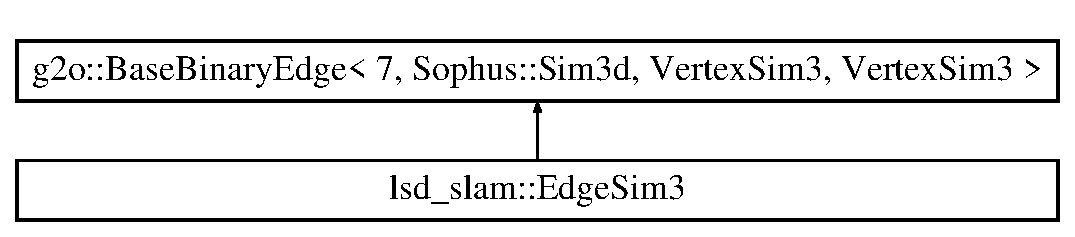
\includegraphics[height=2.000000cm]{classlsd__slam_1_1_edge_sim3}
\end{center}
\end{figure}
\subsection*{Public Member Functions}
\begin{DoxyCompactItemize}
\item 
\hypertarget{classlsd__slam_1_1_edge_sim3_a2dd83a55e96d132bf204d2defe9672e0}{virtual bool {\bfseries read} (std\-::istream \&is)}\label{classlsd__slam_1_1_edge_sim3_a2dd83a55e96d132bf204d2defe9672e0}

\item 
\hypertarget{classlsd__slam_1_1_edge_sim3_afebade8f066f00a7cecd6637ae08d7a3}{virtual bool {\bfseries write} (std\-::ostream \&os) const }\label{classlsd__slam_1_1_edge_sim3_afebade8f066f00a7cecd6637ae08d7a3}

\item 
\hypertarget{classlsd__slam_1_1_edge_sim3_acdd278a37d942e7dc939adcf77644ad3}{void {\bfseries compute\-Error} ()}\label{classlsd__slam_1_1_edge_sim3_acdd278a37d942e7dc939adcf77644ad3}

\item 
\hypertarget{classlsd__slam_1_1_edge_sim3_a625da0349759c6412e24bcae54fdd02c}{void {\bfseries linearize\-Oplus} ()}\label{classlsd__slam_1_1_edge_sim3_a625da0349759c6412e24bcae54fdd02c}

\item 
\hypertarget{classlsd__slam_1_1_edge_sim3_a7acac082215def62ac785981774e219a}{virtual void {\bfseries set\-Measurement} (const Sophus\-::\-Sim3d \&m)}\label{classlsd__slam_1_1_edge_sim3_a7acac082215def62ac785981774e219a}

\item 
\hypertarget{classlsd__slam_1_1_edge_sim3_adf8397eef67232b720b462142580f0ef}{virtual bool {\bfseries set\-Measurement\-Data} (const double $\ast$m)}\label{classlsd__slam_1_1_edge_sim3_adf8397eef67232b720b462142580f0ef}

\item 
\hypertarget{classlsd__slam_1_1_edge_sim3_a074025100cbd539638437ce36994235c}{virtual bool {\bfseries set\-Measurement\-From\-State} ()}\label{classlsd__slam_1_1_edge_sim3_a074025100cbd539638437ce36994235c}

\item 
\hypertarget{classlsd__slam_1_1_edge_sim3_a6c606aa6b9a946bc3c1927839b345a1d}{virtual double {\bfseries initial\-Estimate\-Possible} (const g2o\-::\-Optimizable\-Graph\-::\-Vertex\-Set \&, g2o\-::\-Optimizable\-Graph\-::\-Vertex $\ast$)}\label{classlsd__slam_1_1_edge_sim3_a6c606aa6b9a946bc3c1927839b345a1d}

\item 
\hypertarget{classlsd__slam_1_1_edge_sim3_a927bd86859a9f21bdab9a9eeba53eec4}{virtual void {\bfseries initial\-Estimate} (const g2o\-::\-Optimizable\-Graph\-::\-Vertex\-Set \&from, g2o\-::\-Optimizable\-Graph\-::\-Vertex $\ast$)}\label{classlsd__slam_1_1_edge_sim3_a927bd86859a9f21bdab9a9eeba53eec4}

\end{DoxyCompactItemize}
\subsection*{Protected Attributes}
\begin{DoxyCompactItemize}
\item 
\hypertarget{classlsd__slam_1_1_edge_sim3_a22bd0dcc7b4465e069a0d12aa32e2ff4}{Sophus\-::\-Sim3d {\bfseries \-\_\-inverse\-Measurement}}\label{classlsd__slam_1_1_edge_sim3_a22bd0dcc7b4465e069a0d12aa32e2ff4}

\end{DoxyCompactItemize}


\subsection{Detailed Description}
7\-D edge between two Vertex7 

The documentation for this class was generated from the following files\-:\begin{DoxyCompactItemize}
\item 
/home/king/rgbd-\/slam-\/lets-\/do-\/it/9-\/doxygen/lsd\-\_\-slam/lsd\-\_\-slam\-\_\-core/src/\-Global\-Mapping/g2o\-Type\-Sim3\-Sophus.\-h\item 
/home/king/rgbd-\/slam-\/lets-\/do-\/it/9-\/doxygen/lsd\-\_\-slam/lsd\-\_\-slam\-\_\-core/src/\-Global\-Mapping/g2o\-Type\-Sim3\-Sophus.\-cpp\end{DoxyCompactItemize}

\hypertarget{classlsd__slam_1_1_frame}{\section{lsd\-\_\-slam\-:\-:Frame Class Reference}
\label{classlsd__slam_1_1_frame}\index{lsd\-\_\-slam\-::\-Frame@{lsd\-\_\-slam\-::\-Frame}}
}
\subsection*{Public Types}
\begin{DoxyCompactItemize}
\item 
enum \hyperlink{classlsd__slam_1_1_frame_a91c2bcdbabb5db67344b5379588e6990}{Data\-Flags} \{ \\*
{\bfseries I\-M\-A\-G\-E} = 1$<$$<$0, 
{\bfseries G\-R\-A\-D\-I\-E\-N\-T\-S} = 1$<$$<$1, 
{\bfseries M\-A\-X\-\_\-\-G\-R\-A\-D\-I\-E\-N\-T\-S} = 1$<$$<$2, 
{\bfseries I\-D\-E\-P\-T\-H} = 1$<$$<$3, 
\\*
{\bfseries I\-D\-E\-P\-T\-H\-\_\-\-V\-A\-R} = 1$<$$<$4, 
{\bfseries R\-E\-F\-\_\-\-I\-D} = 1$<$$<$5, 
{\bfseries A\-L\-L} = I\-M\-A\-G\-E $\vert$ G\-R\-A\-D\-I\-E\-N\-T\-S $\vert$ M\-A\-X\-\_\-\-G\-R\-A\-D\-I\-E\-N\-T\-S $\vert$ I\-D\-E\-P\-T\-H $\vert$ I\-D\-E\-P\-T\-H\-\_\-\-V\-A\-R $\vert$ R\-E\-F\-\_\-\-I\-D
 \}
\end{DoxyCompactItemize}
\subsection*{Public Member Functions}
\begin{DoxyCompactItemize}
\item 
\hypertarget{classlsd__slam_1_1_frame_afe0e4c4a37577da20ae9ddd5a854f29d}{{\bfseries Frame} (int \hyperlink{classlsd__slam_1_1_frame_a6d38d40cd9a68d253bcb3cab2ddfa068}{id}, int \hyperlink{classlsd__slam_1_1_frame_a3f14a1c43b6cb21d31274f880b0bf36b}{width}, int \hyperlink{classlsd__slam_1_1_frame_a014d19bf6ffba0f0c0b8b684f9afb0b0}{height}, const Eigen\-::\-Matrix3f \&\hyperlink{classlsd__slam_1_1_frame_adeb235dc3e4a4d8fcf622b5771299c31}{K}, double \hyperlink{classlsd__slam_1_1_frame_a7124f3e1da6e9db387a3f89706225b47}{timestamp}, const unsigned char $\ast$image)}\label{classlsd__slam_1_1_frame_afe0e4c4a37577da20ae9ddd5a854f29d}

\item 
\hypertarget{classlsd__slam_1_1_frame_aeefefa841f84ffa5a2a9a31c5eefe9c0}{{\bfseries Frame} (int \hyperlink{classlsd__slam_1_1_frame_a6d38d40cd9a68d253bcb3cab2ddfa068}{id}, int \hyperlink{classlsd__slam_1_1_frame_a3f14a1c43b6cb21d31274f880b0bf36b}{width}, int \hyperlink{classlsd__slam_1_1_frame_a014d19bf6ffba0f0c0b8b684f9afb0b0}{height}, const Eigen\-::\-Matrix3f \&\hyperlink{classlsd__slam_1_1_frame_adeb235dc3e4a4d8fcf622b5771299c31}{K}, double \hyperlink{classlsd__slam_1_1_frame_a7124f3e1da6e9db387a3f89706225b47}{timestamp}, const float $\ast$image)}\label{classlsd__slam_1_1_frame_aeefefa841f84ffa5a2a9a31c5eefe9c0}

\item 
void \hyperlink{classlsd__slam_1_1_frame_aa869fc645781090678dc61399ef26f73}{set\-Depth} (const \hyperlink{classlsd__slam_1_1_depth_map_pixel_hypothesis}{Depth\-Map\-Pixel\-Hypothesis} $\ast$new\-Depth)
\item 
void \hyperlink{classlsd__slam_1_1_frame_a4ff87802d5bcafda551ffb2506f7192e}{calculate\-Mean\-Information} ()
\item 
void \hyperlink{classlsd__slam_1_1_frame_a7e563deb5eadcaddc85d7618bb021b1b}{set\-Depth\-From\-Ground\-Truth} (const float $\ast$depth, float cov\-\_\-scale=1.\-0f)
\item 
void \hyperlink{classlsd__slam_1_1_frame_a377c85038536721d99473f810cb45241}{prepare\-For\-Stereo\-With} (\hyperlink{classlsd__slam_1_1_frame}{Frame} $\ast$other, Sim3 this\-To\-Other, const Eigen\-::\-Matrix3f \&\hyperlink{classlsd__slam_1_1_frame_adeb235dc3e4a4d8fcf622b5771299c31}{K}, const int level)
\item 
int \hyperlink{classlsd__slam_1_1_frame_a6d38d40cd9a68d253bcb3cab2ddfa068}{id} () const 
\item 
int \hyperlink{classlsd__slam_1_1_frame_a3f14a1c43b6cb21d31274f880b0bf36b}{width} (int level=0) const 
\item 
int \hyperlink{classlsd__slam_1_1_frame_a014d19bf6ffba0f0c0b8b684f9afb0b0}{height} (int level=0) const 
\item 
const Eigen\-::\-Matrix3f \& \hyperlink{classlsd__slam_1_1_frame_adeb235dc3e4a4d8fcf622b5771299c31}{K} (int level=0) const 
\item 
const Eigen\-::\-Matrix3f \& \hyperlink{classlsd__slam_1_1_frame_af32c050a1ada7d6c22aa8df04fd94085}{K\-Inv} (int level=0) const 
\item 
float \hyperlink{classlsd__slam_1_1_frame_aaa552f594a3e712b981762719d652359}{fx} (int level=0) const 
\item 
float \hyperlink{classlsd__slam_1_1_frame_af8a9e82339d7f20a380a47d27cdeb01e}{fy} (int level=0) const 
\item 
float \hyperlink{classlsd__slam_1_1_frame_a8d46588a32aa5feb71f771f267dc432d}{cx} (int level=0) const 
\item 
float \hyperlink{classlsd__slam_1_1_frame_a2732f1bad0442085b11f3552a2fd0525}{cy} (int level=0) const 
\item 
float \hyperlink{classlsd__slam_1_1_frame_a9d98889a6a367e862f28b4a035604f46}{fx\-Inv} (int level=0) const 
\item 
float \hyperlink{classlsd__slam_1_1_frame_ab5c98941622d0f0470381a8ed2f833c1}{fy\-Inv} (int level=0) const 
\item 
float \hyperlink{classlsd__slam_1_1_frame_a4690556800b10f98c18a2fada62ae62b}{cx\-Inv} (int level=0) const 
\item 
float \hyperlink{classlsd__slam_1_1_frame_aae9fa687e7e515ba009a5fe5a617bf75}{cy\-Inv} (int level=0) const 
\item 
double \hyperlink{classlsd__slam_1_1_frame_a7124f3e1da6e9db387a3f89706225b47}{timestamp} () const 
\item 
\hypertarget{classlsd__slam_1_1_frame_a9306307027bbe62b973c0b138216b456}{float $\ast$ {\bfseries image} (int level=0)}\label{classlsd__slam_1_1_frame_a9306307027bbe62b973c0b138216b456}

\item 
\hypertarget{classlsd__slam_1_1_frame_a2c31baa0cea975fb73ccf80d92f7a5de}{const Eigen\-::\-Vector4f $\ast$ {\bfseries gradients} (int level=0)}\label{classlsd__slam_1_1_frame_a2c31baa0cea975fb73ccf80d92f7a5de}

\item 
\hypertarget{classlsd__slam_1_1_frame_a0b26845d846249e909e6ab0adc022ebf}{const float $\ast$ {\bfseries max\-Gradients} (int level=0)}\label{classlsd__slam_1_1_frame_a0b26845d846249e909e6ab0adc022ebf}

\item 
\hypertarget{classlsd__slam_1_1_frame_abe0ec6e93823ae0a31e73100a8b73940}{bool {\bfseries has\-I\-Depth\-Been\-Set} () const }\label{classlsd__slam_1_1_frame_abe0ec6e93823ae0a31e73100a8b73940}

\item 
\hypertarget{classlsd__slam_1_1_frame_ad78d873de1adfd4ab3268c50b1d462c7}{const float $\ast$ {\bfseries idepth} (int level=0)}\label{classlsd__slam_1_1_frame_ad78d873de1adfd4ab3268c50b1d462c7}

\item 
\hypertarget{classlsd__slam_1_1_frame_aa3fb7f275b5da621c039a6746b905770}{const float $\ast$ {\bfseries idepth\-Var} (int level=0)}\label{classlsd__slam_1_1_frame_aa3fb7f275b5da621c039a6746b905770}

\item 
\hypertarget{classlsd__slam_1_1_frame_a51cfb8cc35140eee3283021d97496db6}{const unsigned char $\ast$ {\bfseries validity\-\_\-re\-Act} ()}\label{classlsd__slam_1_1_frame_a51cfb8cc35140eee3283021d97496db6}

\item 
\hypertarget{classlsd__slam_1_1_frame_adac400f4b48f3d5ea20ee4ac8ea5ad8e}{const float $\ast$ {\bfseries idepth\-\_\-re\-Act} ()}\label{classlsd__slam_1_1_frame_adac400f4b48f3d5ea20ee4ac8ea5ad8e}

\item 
\hypertarget{classlsd__slam_1_1_frame_a8e128c8fdc004bd808c365c1ea38c9bd}{const float $\ast$ {\bfseries idepth\-Var\-\_\-re\-Act} ()}\label{classlsd__slam_1_1_frame_a8e128c8fdc004bd808c365c1ea38c9bd}

\item 
\hypertarget{classlsd__slam_1_1_frame_a8c3122c4784b9a8ae66210205bf531d1}{bool $\ast$ {\bfseries ref\-Pixel\-Was\-Good} ()}\label{classlsd__slam_1_1_frame_a8c3122c4784b9a8ae66210205bf531d1}

\item 
\hypertarget{classlsd__slam_1_1_frame_adb19bd5898e7d6e8ceb9a826096d166e}{bool $\ast$ {\bfseries ref\-Pixel\-Was\-Good\-No\-Create} ()}\label{classlsd__slam_1_1_frame_adb19bd5898e7d6e8ceb9a826096d166e}

\item 
\hypertarget{classlsd__slam_1_1_frame_a89c328ba630444fa4324c2c33b3141f3}{void {\bfseries clear\-\_\-ref\-Pixel\-Was\-Good} ()}\label{classlsd__slam_1_1_frame_a89c328ba630444fa4324c2c33b3141f3}

\item 
\hypertarget{classlsd__slam_1_1_frame_a3e56b78f4f1989fa15fa3da5dfb97c81}{void {\bfseries set\-Perma\-Ref} (\hyperlink{classlsd__slam_1_1_tracking_reference}{Tracking\-Reference} $\ast$reference)}\label{classlsd__slam_1_1_frame_a3e56b78f4f1989fa15fa3da5dfb97c81}

\item 
\hypertarget{classlsd__slam_1_1_frame_aab79f2a5a9f59c2cf2b9714ad48c53ae}{void {\bfseries take\-Re\-Activation\-Data} (\hyperlink{classlsd__slam_1_1_depth_map_pixel_hypothesis}{Depth\-Map\-Pixel\-Hypothesis} $\ast$depth\-Map)}\label{classlsd__slam_1_1_frame_aab79f2a5a9f59c2cf2b9714ad48c53ae}

\item 
\hypertarget{classlsd__slam_1_1_frame_af73ccb75e1e449d9a8f2044246ee3530}{boost\-::shared\-\_\-lock\\*
$<$ boost\-::shared\-\_\-mutex $>$ {\bfseries get\-Active\-Lock} ()}\label{classlsd__slam_1_1_frame_af73ccb75e1e449d9a8f2044246ee3530}

\item 
\hypertarget{classlsd__slam_1_1_frame_a0f4a92d51569c280e4b37acbf562ea47}{Sim3 {\bfseries get\-Scaled\-Cam\-To\-World} (int num=0)}\label{classlsd__slam_1_1_frame_a0f4a92d51569c280e4b37acbf562ea47}

\item 
\hypertarget{classlsd__slam_1_1_frame_a013921be6869702deac98090a8c9033c}{bool {\bfseries has\-Tracking\-Parent} ()}\label{classlsd__slam_1_1_frame_a013921be6869702deac98090a8c9033c}

\item 
\hypertarget{classlsd__slam_1_1_frame_ae337afb7e308ff6d9be3ffa354fc66d6}{\hyperlink{classlsd__slam_1_1_frame}{Frame} $\ast$ {\bfseries get\-Tracking\-Parent} ()}\label{classlsd__slam_1_1_frame_ae337afb7e308ff6d9be3ffa354fc66d6}

\end{DoxyCompactItemize}
\subsection*{Public Attributes}
\begin{DoxyCompactItemize}
\item 
\hypertarget{classlsd__slam_1_1_frame_a9e446e7abf6fc1e988594935dad9072b}{\hyperlink{classlsd__slam_1_1_frame_pose_struct}{Frame\-Pose\-Struct} $\ast$ {\bfseries pose}}\label{classlsd__slam_1_1_frame_a9e446e7abf6fc1e988594935dad9072b}

\item 
\hypertarget{classlsd__slam_1_1_frame_a013a9e6ef9bd7d72f46df32dbd261861}{Sim3 {\bfseries last\-Constraint\-Tracked\-Cam\-To\-World}}\label{classlsd__slam_1_1_frame_a013a9e6ef9bd7d72f46df32dbd261861}

\item 
std\-::unordered\-\_\-set$<$ \hyperlink{classlsd__slam_1_1_frame}{Frame} \\*
$\ast$, std\-::hash$<$ \hyperlink{classlsd__slam_1_1_frame}{Frame} $\ast$ $>$\\*
, std\-::equal\-\_\-to$<$ \hyperlink{classlsd__slam_1_1_frame}{Frame} $\ast$ $>$\\*
, Eigen\-::aligned\-\_\-allocator\\*
$<$ \hyperlink{classlsd__slam_1_1_frame}{Frame} $\ast$ $>$ $>$ \hyperlink{classlsd__slam_1_1_frame_ac0beb1665cd6caecfef8f6103203c147}{neighbors}
\item 
std\-::unordered\-\_\-multimap$<$ \hyperlink{classlsd__slam_1_1_frame}{Frame} \\*
$\ast$, Sim3, std\-::hash$<$ \hyperlink{classlsd__slam_1_1_frame}{Frame} $\ast$ $>$\\*
, std\-::equal\-\_\-to$<$ \hyperlink{classlsd__slam_1_1_frame}{Frame} $\ast$ $>$\\*
, Eigen\-::aligned\-\_\-allocator\\*
$<$ std\-::pair$<$ const \hyperlink{classlsd__slam_1_1_frame}{Frame} \\*
$\ast$, Sim3 $>$ $>$ $>$ \hyperlink{classlsd__slam_1_1_frame_a71811be54c6d349c9f13e50361b14718}{tracking\-Failed}
\item 
\hypertarget{classlsd__slam_1_1_frame_a2447e3447316b2803b20542e70e10785}{bool {\bfseries depth\-Has\-Been\-Updated\-Flag}}\label{classlsd__slam_1_1_frame_a2447e3447316b2803b20542e70e10785}

\item 
\hypertarget{classlsd__slam_1_1_frame_af05033d502e07e33f61908c7b0f6ea17}{boost\-::mutex {\bfseries perma\-Ref\-\_\-mutex}}\label{classlsd__slam_1_1_frame_af05033d502e07e33f61908c7b0f6ea17}

\item 
\hypertarget{classlsd__slam_1_1_frame_a18011d25126f677273f88ba227e32278}{Eigen\-::\-Vector3f $\ast$ {\bfseries perma\-Ref\-\_\-pos\-Data}}\label{classlsd__slam_1_1_frame_a18011d25126f677273f88ba227e32278}

\item 
\hypertarget{classlsd__slam_1_1_frame_ab604a46aff3018462fe4171fc9cbde69}{Eigen\-::\-Vector2f $\ast$ {\bfseries perma\-Ref\-\_\-color\-And\-Var\-Data}}\label{classlsd__slam_1_1_frame_ab604a46aff3018462fe4171fc9cbde69}

\item 
\hypertarget{classlsd__slam_1_1_frame_ae2968ee29976f194c3c8c552f7ebf3b7}{int {\bfseries perma\-Ref\-Num\-Pts}}\label{classlsd__slam_1_1_frame_ae2968ee29976f194c3c8c552f7ebf3b7}

\item 
\hypertarget{classlsd__slam_1_1_frame_a45c1d420e51ecd4b078bb5992ef9c72f}{int {\bfseries reference\-I\-D}}\label{classlsd__slam_1_1_frame_a45c1d420e51ecd4b078bb5992ef9c72f}

\item 
\hypertarget{classlsd__slam_1_1_frame_a98746a5422a8afa51dfc5fc21d4e4cc6}{int {\bfseries reference\-Level}}\label{classlsd__slam_1_1_frame_a98746a5422a8afa51dfc5fc21d4e4cc6}

\item 
\hypertarget{classlsd__slam_1_1_frame_a400b62f479205f178a23cd48f41186d0}{float {\bfseries dist\-Squared}}\label{classlsd__slam_1_1_frame_a400b62f479205f178a23cd48f41186d0}

\item 
\hypertarget{classlsd__slam_1_1_frame_aa5422a17806f94238eb4b0a997f84d3c}{Eigen\-::\-Matrix3f {\bfseries K\-\_\-other\-To\-This\-\_\-\-R}}\label{classlsd__slam_1_1_frame_aa5422a17806f94238eb4b0a997f84d3c}

\item 
\hypertarget{classlsd__slam_1_1_frame_a299bcddaca0539b927cc0e3a6ec5739b}{Eigen\-::\-Vector3f {\bfseries K\-\_\-other\-To\-This\-\_\-t}}\label{classlsd__slam_1_1_frame_a299bcddaca0539b927cc0e3a6ec5739b}

\item 
\hypertarget{classlsd__slam_1_1_frame_ac60ac357b2988ee6ae78cc0ea9030d77}{Eigen\-::\-Vector3f {\bfseries other\-To\-This\-\_\-t}}\label{classlsd__slam_1_1_frame_ac60ac357b2988ee6ae78cc0ea9030d77}

\item 
\hypertarget{classlsd__slam_1_1_frame_ae67bd56784580e5bba78c78c54c79513}{Eigen\-::\-Vector3f {\bfseries K\-\_\-this\-To\-Other\-\_\-t}}\label{classlsd__slam_1_1_frame_ae67bd56784580e5bba78c78c54c79513}

\item 
\hypertarget{classlsd__slam_1_1_frame_a99da615609b7b2470447dbc00d022543}{Eigen\-::\-Matrix3f {\bfseries this\-To\-Other\-\_\-\-R}}\label{classlsd__slam_1_1_frame_a99da615609b7b2470447dbc00d022543}

\item 
\hypertarget{classlsd__slam_1_1_frame_acc99c43a91d9a928885536632ed9b701}{Eigen\-::\-Vector3f {\bfseries other\-To\-This\-\_\-\-R\-\_\-row0}}\label{classlsd__slam_1_1_frame_acc99c43a91d9a928885536632ed9b701}

\item 
\hypertarget{classlsd__slam_1_1_frame_a9e73fe70e8b2b845d83663513a7cee31}{Eigen\-::\-Vector3f {\bfseries other\-To\-This\-\_\-\-R\-\_\-row1}}\label{classlsd__slam_1_1_frame_a9e73fe70e8b2b845d83663513a7cee31}

\item 
\hypertarget{classlsd__slam_1_1_frame_aa94f79b5dd632a55a7069a57f45927a1}{Eigen\-::\-Vector3f {\bfseries other\-To\-This\-\_\-\-R\-\_\-row2}}\label{classlsd__slam_1_1_frame_aa94f79b5dd632a55a7069a57f45927a1}

\item 
\hypertarget{classlsd__slam_1_1_frame_a61b36968ff859b298eda25741c4d98a2}{Eigen\-::\-Vector3f {\bfseries this\-To\-Other\-\_\-t}}\label{classlsd__slam_1_1_frame_a61b36968ff859b298eda25741c4d98a2}

\item 
\hypertarget{classlsd__slam_1_1_frame_ac58ef4a32c0d5052e3722da6ff84d07d}{float {\bfseries initial\-Tracked\-Residual}}\label{classlsd__slam_1_1_frame_ac58ef4a32c0d5052e3722da6ff84d07d}

\item 
\hypertarget{classlsd__slam_1_1_frame_a0e33cc989142a9266f582df4931fbd52}{int {\bfseries num\-Frames\-Tracked\-On\-This}}\label{classlsd__slam_1_1_frame_a0e33cc989142a9266f582df4931fbd52}

\item 
\hypertarget{classlsd__slam_1_1_frame_a722bd8b07e962b6de142519f38405628}{int {\bfseries num\-Mapped\-On\-This}}\label{classlsd__slam_1_1_frame_a722bd8b07e962b6de142519f38405628}

\item 
\hypertarget{classlsd__slam_1_1_frame_a18830417f9d1cdd547145fdd3d8de297}{int {\bfseries num\-Mapped\-On\-This\-Total}}\label{classlsd__slam_1_1_frame_a18830417f9d1cdd547145fdd3d8de297}

\item 
\hypertarget{classlsd__slam_1_1_frame_a8b1c8af671c71ea2d4dc934e5276c2b4}{float {\bfseries mean\-Idepth}}\label{classlsd__slam_1_1_frame_a8b1c8af671c71ea2d4dc934e5276c2b4}

\item 
\hypertarget{classlsd__slam_1_1_frame_a5d9849821321c33e90281e84d95abf37}{int {\bfseries num\-Points}}\label{classlsd__slam_1_1_frame_a5d9849821321c33e90281e84d95abf37}

\item 
\hypertarget{classlsd__slam_1_1_frame_afd88bf74afcd11574145358eac8da4b0}{int {\bfseries idx\-In\-Keyframes}}\label{classlsd__slam_1_1_frame_afd88bf74afcd11574145358eac8da4b0}

\item 
\hypertarget{classlsd__slam_1_1_frame_a6b06772b4f54122c098b9044ffd9876c}{float {\bfseries edge\-Error\-Sum}}\label{classlsd__slam_1_1_frame_a6b06772b4f54122c098b9044ffd9876c}

\item 
\hypertarget{classlsd__slam_1_1_frame_ac1d94c23c259fa087f37cf9607253010}{float {\bfseries edges\-Num}}\label{classlsd__slam_1_1_frame_ac1d94c23c259fa087f37cf9607253010}

\item 
\hypertarget{classlsd__slam_1_1_frame_a8f73786134dcc966d8f8f4ac8f7aa58c}{int {\bfseries num\-Mappable\-Pixels}}\label{classlsd__slam_1_1_frame_a8f73786134dcc966d8f8f4ac8f7aa58c}

\item 
\hypertarget{classlsd__slam_1_1_frame_ab54ac9e919e344553900a8f89f383226}{float {\bfseries mean\-Information}}\label{classlsd__slam_1_1_frame_ab54ac9e919e344553900a8f89f383226}

\end{DoxyCompactItemize}
\subsection*{Friends}
\begin{DoxyCompactItemize}
\item 
\hypertarget{classlsd__slam_1_1_frame_a301c44f1a60e7b77092f38610c22f920}{class {\bfseries Frame\-Memory}}\label{classlsd__slam_1_1_frame_a301c44f1a60e7b77092f38610c22f920}

\end{DoxyCompactItemize}


\subsection{Member Enumeration Documentation}
\hypertarget{classlsd__slam_1_1_frame_a91c2bcdbabb5db67344b5379588e6990}{\index{lsd\-\_\-slam\-::\-Frame@{lsd\-\_\-slam\-::\-Frame}!Data\-Flags@{Data\-Flags}}
\index{Data\-Flags@{Data\-Flags}!lsd_slam::Frame@{lsd\-\_\-slam\-::\-Frame}}
\subsubsection[{Data\-Flags}]{\setlength{\rightskip}{0pt plus 5cm}enum {\bf lsd\-\_\-slam\-::\-Frame\-::\-Data\-Flags}}}\label{classlsd__slam_1_1_frame_a91c2bcdbabb5db67344b5379588e6990}
Flags for use with require() and require\-Pyramid(). See the \hyperlink{classlsd__slam_1_1_frame}{Frame} class documentation for their exact meaning. 

\subsection{Member Function Documentation}
\hypertarget{classlsd__slam_1_1_frame_a4ff87802d5bcafda551ffb2506f7192e}{\index{lsd\-\_\-slam\-::\-Frame@{lsd\-\_\-slam\-::\-Frame}!calculate\-Mean\-Information@{calculate\-Mean\-Information}}
\index{calculate\-Mean\-Information@{calculate\-Mean\-Information}!lsd_slam::Frame@{lsd\-\_\-slam\-::\-Frame}}
\subsubsection[{calculate\-Mean\-Information}]{\setlength{\rightskip}{0pt plus 5cm}void lsd\-\_\-slam\-::\-Frame\-::calculate\-Mean\-Information (
\begin{DoxyParamCaption}
{}
\end{DoxyParamCaption}
)}}\label{classlsd__slam_1_1_frame_a4ff87802d5bcafda551ffb2506f7192e}
Calculates mean information for statistical purposes. \hypertarget{classlsd__slam_1_1_frame_a8d46588a32aa5feb71f771f267dc432d}{\index{lsd\-\_\-slam\-::\-Frame@{lsd\-\_\-slam\-::\-Frame}!cx@{cx}}
\index{cx@{cx}!lsd_slam::Frame@{lsd\-\_\-slam\-::\-Frame}}
\subsubsection[{cx}]{\setlength{\rightskip}{0pt plus 5cm}float lsd\-\_\-slam\-::\-Frame\-::cx (
\begin{DoxyParamCaption}
\item[{int}]{level = {\ttfamily 0}}
\end{DoxyParamCaption}
) const\hspace{0.3cm}{\ttfamily [inline]}}}\label{classlsd__slam_1_1_frame_a8d46588a32aa5feb71f771f267dc432d}
Returns K(0, 2). \hypertarget{classlsd__slam_1_1_frame_a4690556800b10f98c18a2fada62ae62b}{\index{lsd\-\_\-slam\-::\-Frame@{lsd\-\_\-slam\-::\-Frame}!cx\-Inv@{cx\-Inv}}
\index{cx\-Inv@{cx\-Inv}!lsd_slam::Frame@{lsd\-\_\-slam\-::\-Frame}}
\subsubsection[{cx\-Inv}]{\setlength{\rightskip}{0pt plus 5cm}float lsd\-\_\-slam\-::\-Frame\-::cx\-Inv (
\begin{DoxyParamCaption}
\item[{int}]{level = {\ttfamily 0}}
\end{DoxyParamCaption}
) const\hspace{0.3cm}{\ttfamily [inline]}}}\label{classlsd__slam_1_1_frame_a4690556800b10f98c18a2fada62ae62b}
Returns K\-Inv(0, 2). \hypertarget{classlsd__slam_1_1_frame_a2732f1bad0442085b11f3552a2fd0525}{\index{lsd\-\_\-slam\-::\-Frame@{lsd\-\_\-slam\-::\-Frame}!cy@{cy}}
\index{cy@{cy}!lsd_slam::Frame@{lsd\-\_\-slam\-::\-Frame}}
\subsubsection[{cy}]{\setlength{\rightskip}{0pt plus 5cm}float lsd\-\_\-slam\-::\-Frame\-::cy (
\begin{DoxyParamCaption}
\item[{int}]{level = {\ttfamily 0}}
\end{DoxyParamCaption}
) const\hspace{0.3cm}{\ttfamily [inline]}}}\label{classlsd__slam_1_1_frame_a2732f1bad0442085b11f3552a2fd0525}
Returns K(1, 2). \hypertarget{classlsd__slam_1_1_frame_aae9fa687e7e515ba009a5fe5a617bf75}{\index{lsd\-\_\-slam\-::\-Frame@{lsd\-\_\-slam\-::\-Frame}!cy\-Inv@{cy\-Inv}}
\index{cy\-Inv@{cy\-Inv}!lsd_slam::Frame@{lsd\-\_\-slam\-::\-Frame}}
\subsubsection[{cy\-Inv}]{\setlength{\rightskip}{0pt plus 5cm}float lsd\-\_\-slam\-::\-Frame\-::cy\-Inv (
\begin{DoxyParamCaption}
\item[{int}]{level = {\ttfamily 0}}
\end{DoxyParamCaption}
) const\hspace{0.3cm}{\ttfamily [inline]}}}\label{classlsd__slam_1_1_frame_aae9fa687e7e515ba009a5fe5a617bf75}
Returns K\-Inv(1, 2). \hypertarget{classlsd__slam_1_1_frame_aaa552f594a3e712b981762719d652359}{\index{lsd\-\_\-slam\-::\-Frame@{lsd\-\_\-slam\-::\-Frame}!fx@{fx}}
\index{fx@{fx}!lsd_slam::Frame@{lsd\-\_\-slam\-::\-Frame}}
\subsubsection[{fx}]{\setlength{\rightskip}{0pt plus 5cm}float lsd\-\_\-slam\-::\-Frame\-::fx (
\begin{DoxyParamCaption}
\item[{int}]{level = {\ttfamily 0}}
\end{DoxyParamCaption}
) const\hspace{0.3cm}{\ttfamily [inline]}}}\label{classlsd__slam_1_1_frame_aaa552f594a3e712b981762719d652359}
Returns K(0, 0). \hypertarget{classlsd__slam_1_1_frame_a9d98889a6a367e862f28b4a035604f46}{\index{lsd\-\_\-slam\-::\-Frame@{lsd\-\_\-slam\-::\-Frame}!fx\-Inv@{fx\-Inv}}
\index{fx\-Inv@{fx\-Inv}!lsd_slam::Frame@{lsd\-\_\-slam\-::\-Frame}}
\subsubsection[{fx\-Inv}]{\setlength{\rightskip}{0pt plus 5cm}float lsd\-\_\-slam\-::\-Frame\-::fx\-Inv (
\begin{DoxyParamCaption}
\item[{int}]{level = {\ttfamily 0}}
\end{DoxyParamCaption}
) const\hspace{0.3cm}{\ttfamily [inline]}}}\label{classlsd__slam_1_1_frame_a9d98889a6a367e862f28b4a035604f46}
Returns K\-Inv(0, 0). \hypertarget{classlsd__slam_1_1_frame_af8a9e82339d7f20a380a47d27cdeb01e}{\index{lsd\-\_\-slam\-::\-Frame@{lsd\-\_\-slam\-::\-Frame}!fy@{fy}}
\index{fy@{fy}!lsd_slam::Frame@{lsd\-\_\-slam\-::\-Frame}}
\subsubsection[{fy}]{\setlength{\rightskip}{0pt plus 5cm}float lsd\-\_\-slam\-::\-Frame\-::fy (
\begin{DoxyParamCaption}
\item[{int}]{level = {\ttfamily 0}}
\end{DoxyParamCaption}
) const\hspace{0.3cm}{\ttfamily [inline]}}}\label{classlsd__slam_1_1_frame_af8a9e82339d7f20a380a47d27cdeb01e}
Returns K(1, 1). \hypertarget{classlsd__slam_1_1_frame_ab5c98941622d0f0470381a8ed2f833c1}{\index{lsd\-\_\-slam\-::\-Frame@{lsd\-\_\-slam\-::\-Frame}!fy\-Inv@{fy\-Inv}}
\index{fy\-Inv@{fy\-Inv}!lsd_slam::Frame@{lsd\-\_\-slam\-::\-Frame}}
\subsubsection[{fy\-Inv}]{\setlength{\rightskip}{0pt plus 5cm}float lsd\-\_\-slam\-::\-Frame\-::fy\-Inv (
\begin{DoxyParamCaption}
\item[{int}]{level = {\ttfamily 0}}
\end{DoxyParamCaption}
) const\hspace{0.3cm}{\ttfamily [inline]}}}\label{classlsd__slam_1_1_frame_ab5c98941622d0f0470381a8ed2f833c1}
Returns K\-Inv(1, 1). \hypertarget{classlsd__slam_1_1_frame_a014d19bf6ffba0f0c0b8b684f9afb0b0}{\index{lsd\-\_\-slam\-::\-Frame@{lsd\-\_\-slam\-::\-Frame}!height@{height}}
\index{height@{height}!lsd_slam::Frame@{lsd\-\_\-slam\-::\-Frame}}
\subsubsection[{height}]{\setlength{\rightskip}{0pt plus 5cm}int lsd\-\_\-slam\-::\-Frame\-::height (
\begin{DoxyParamCaption}
\item[{int}]{level = {\ttfamily 0}}
\end{DoxyParamCaption}
) const\hspace{0.3cm}{\ttfamily [inline]}}}\label{classlsd__slam_1_1_frame_a014d19bf6ffba0f0c0b8b684f9afb0b0}
Returns the frame's image height. \hypertarget{classlsd__slam_1_1_frame_a6d38d40cd9a68d253bcb3cab2ddfa068}{\index{lsd\-\_\-slam\-::\-Frame@{lsd\-\_\-slam\-::\-Frame}!id@{id}}
\index{id@{id}!lsd_slam::Frame@{lsd\-\_\-slam\-::\-Frame}}
\subsubsection[{id}]{\setlength{\rightskip}{0pt plus 5cm}int lsd\-\_\-slam\-::\-Frame\-::id (
\begin{DoxyParamCaption}
{}
\end{DoxyParamCaption}
) const\hspace{0.3cm}{\ttfamily [inline]}}}\label{classlsd__slam_1_1_frame_a6d38d40cd9a68d253bcb3cab2ddfa068}
Returns the unique frame id. \hypertarget{classlsd__slam_1_1_frame_adeb235dc3e4a4d8fcf622b5771299c31}{\index{lsd\-\_\-slam\-::\-Frame@{lsd\-\_\-slam\-::\-Frame}!K@{K}}
\index{K@{K}!lsd_slam::Frame@{lsd\-\_\-slam\-::\-Frame}}
\subsubsection[{K}]{\setlength{\rightskip}{0pt plus 5cm}const Eigen\-::\-Matrix3f \& lsd\-\_\-slam\-::\-Frame\-::\-K (
\begin{DoxyParamCaption}
\item[{int}]{level = {\ttfamily 0}}
\end{DoxyParamCaption}
) const\hspace{0.3cm}{\ttfamily [inline]}}}\label{classlsd__slam_1_1_frame_adeb235dc3e4a4d8fcf622b5771299c31}
Returns the frame's intrinsics matrix. \hypertarget{classlsd__slam_1_1_frame_af32c050a1ada7d6c22aa8df04fd94085}{\index{lsd\-\_\-slam\-::\-Frame@{lsd\-\_\-slam\-::\-Frame}!K\-Inv@{K\-Inv}}
\index{K\-Inv@{K\-Inv}!lsd_slam::Frame@{lsd\-\_\-slam\-::\-Frame}}
\subsubsection[{K\-Inv}]{\setlength{\rightskip}{0pt plus 5cm}const Eigen\-::\-Matrix3f \& lsd\-\_\-slam\-::\-Frame\-::\-K\-Inv (
\begin{DoxyParamCaption}
\item[{int}]{level = {\ttfamily 0}}
\end{DoxyParamCaption}
) const\hspace{0.3cm}{\ttfamily [inline]}}}\label{classlsd__slam_1_1_frame_af32c050a1ada7d6c22aa8df04fd94085}
Returns the frame's inverse intrinsics matrix. \hypertarget{classlsd__slam_1_1_frame_a377c85038536721d99473f810cb45241}{\index{lsd\-\_\-slam\-::\-Frame@{lsd\-\_\-slam\-::\-Frame}!prepare\-For\-Stereo\-With@{prepare\-For\-Stereo\-With}}
\index{prepare\-For\-Stereo\-With@{prepare\-For\-Stereo\-With}!lsd_slam::Frame@{lsd\-\_\-slam\-::\-Frame}}
\subsubsection[{prepare\-For\-Stereo\-With}]{\setlength{\rightskip}{0pt plus 5cm}void lsd\-\_\-slam\-::\-Frame\-::prepare\-For\-Stereo\-With (
\begin{DoxyParamCaption}
\item[{{\bf Frame} $\ast$}]{other, }
\item[{Sim3}]{this\-To\-Other, }
\item[{const Eigen\-::\-Matrix3f \&}]{K, }
\item[{const int}]{level}
\end{DoxyParamCaption}
)}}\label{classlsd__slam_1_1_frame_a377c85038536721d99473f810cb45241}
Prepares this frame for stereo comparisons with the other frame (computes some intermediate values that will be needed) \hypertarget{classlsd__slam_1_1_frame_aa869fc645781090678dc61399ef26f73}{\index{lsd\-\_\-slam\-::\-Frame@{lsd\-\_\-slam\-::\-Frame}!set\-Depth@{set\-Depth}}
\index{set\-Depth@{set\-Depth}!lsd_slam::Frame@{lsd\-\_\-slam\-::\-Frame}}
\subsubsection[{set\-Depth}]{\setlength{\rightskip}{0pt plus 5cm}void lsd\-\_\-slam\-::\-Frame\-::set\-Depth (
\begin{DoxyParamCaption}
\item[{const {\bf Depth\-Map\-Pixel\-Hypothesis} $\ast$}]{new\-Depth}
\end{DoxyParamCaption}
)}}\label{classlsd__slam_1_1_frame_aa869fc645781090678dc61399ef26f73}
Sets or updates idepth and idepth\-Var on level zero. Invalidates higher levels. \hypertarget{classlsd__slam_1_1_frame_a7e563deb5eadcaddc85d7618bb021b1b}{\index{lsd\-\_\-slam\-::\-Frame@{lsd\-\_\-slam\-::\-Frame}!set\-Depth\-From\-Ground\-Truth@{set\-Depth\-From\-Ground\-Truth}}
\index{set\-Depth\-From\-Ground\-Truth@{set\-Depth\-From\-Ground\-Truth}!lsd_slam::Frame@{lsd\-\_\-slam\-::\-Frame}}
\subsubsection[{set\-Depth\-From\-Ground\-Truth}]{\setlength{\rightskip}{0pt plus 5cm}void lsd\-\_\-slam\-::\-Frame\-::set\-Depth\-From\-Ground\-Truth (
\begin{DoxyParamCaption}
\item[{const float $\ast$}]{depth, }
\item[{float}]{cov\-\_\-scale = {\ttfamily 1.0f}}
\end{DoxyParamCaption}
)}}\label{classlsd__slam_1_1_frame_a7e563deb5eadcaddc85d7618bb021b1b}
Sets ground truth depth (real, not inverse!) from a float array on level zero. Invalidates higher levels. \hypertarget{classlsd__slam_1_1_frame_a7124f3e1da6e9db387a3f89706225b47}{\index{lsd\-\_\-slam\-::\-Frame@{lsd\-\_\-slam\-::\-Frame}!timestamp@{timestamp}}
\index{timestamp@{timestamp}!lsd_slam::Frame@{lsd\-\_\-slam\-::\-Frame}}
\subsubsection[{timestamp}]{\setlength{\rightskip}{0pt plus 5cm}double lsd\-\_\-slam\-::\-Frame\-::timestamp (
\begin{DoxyParamCaption}
{}
\end{DoxyParamCaption}
) const\hspace{0.3cm}{\ttfamily [inline]}}}\label{classlsd__slam_1_1_frame_a7124f3e1da6e9db387a3f89706225b47}
Returns the frame's recording timestamp. \hypertarget{classlsd__slam_1_1_frame_a3f14a1c43b6cb21d31274f880b0bf36b}{\index{lsd\-\_\-slam\-::\-Frame@{lsd\-\_\-slam\-::\-Frame}!width@{width}}
\index{width@{width}!lsd_slam::Frame@{lsd\-\_\-slam\-::\-Frame}}
\subsubsection[{width}]{\setlength{\rightskip}{0pt plus 5cm}int lsd\-\_\-slam\-::\-Frame\-::width (
\begin{DoxyParamCaption}
\item[{int}]{level = {\ttfamily 0}}
\end{DoxyParamCaption}
) const\hspace{0.3cm}{\ttfamily [inline]}}}\label{classlsd__slam_1_1_frame_a3f14a1c43b6cb21d31274f880b0bf36b}
Returns the frame's image width. 

\subsection{Member Data Documentation}
\hypertarget{classlsd__slam_1_1_frame_ac0beb1665cd6caecfef8f6103203c147}{\index{lsd\-\_\-slam\-::\-Frame@{lsd\-\_\-slam\-::\-Frame}!neighbors@{neighbors}}
\index{neighbors@{neighbors}!lsd_slam::Frame@{lsd\-\_\-slam\-::\-Frame}}
\subsubsection[{neighbors}]{\setlength{\rightskip}{0pt plus 5cm}std\-::unordered\-\_\-set$<$ {\bf Frame}$\ast$, std\-::hash$<${\bf Frame}$\ast$$>$, std\-::equal\-\_\-to$<${\bf Frame}$\ast$$>$, Eigen\-::aligned\-\_\-allocator$<$ {\bf Frame}$\ast$ $>$ $>$ lsd\-\_\-slam\-::\-Frame\-::neighbors}}\label{classlsd__slam_1_1_frame_ac0beb1665cd6caecfef8f6103203c147}
Pointers to all adjacent Frames in graph. empty for non-\/keyframes. \hypertarget{classlsd__slam_1_1_frame_a71811be54c6d349c9f13e50361b14718}{\index{lsd\-\_\-slam\-::\-Frame@{lsd\-\_\-slam\-::\-Frame}!tracking\-Failed@{tracking\-Failed}}
\index{tracking\-Failed@{tracking\-Failed}!lsd_slam::Frame@{lsd\-\_\-slam\-::\-Frame}}
\subsubsection[{tracking\-Failed}]{\setlength{\rightskip}{0pt plus 5cm}std\-::unordered\-\_\-multimap$<$ {\bf Frame}$\ast$, Sim3, std\-::hash$<${\bf Frame}$\ast$$>$, std\-::equal\-\_\-to$<${\bf Frame}$\ast$$>$, Eigen\-::aligned\-\_\-allocator$<$ std\-::pair$<$const {\bf Frame}$\ast$,Sim3$>$ $>$ $>$ lsd\-\_\-slam\-::\-Frame\-::tracking\-Failed}}\label{classlsd__slam_1_1_frame_a71811be54c6d349c9f13e50361b14718}
Multi-\/\-Map indicating for which other keyframes with which initialization tracking failed. 

The documentation for this class was generated from the following files\-:\begin{DoxyCompactItemize}
\item 
/home/king/rgbd-\/slam-\/lets-\/do-\/it/9-\/doxygen/lsd\-\_\-slam/lsd\-\_\-slam\-\_\-core/src/\-Data\-Structures/Frame.\-h\item 
/home/king/rgbd-\/slam-\/lets-\/do-\/it/9-\/doxygen/lsd\-\_\-slam/lsd\-\_\-slam\-\_\-core/src/\-Data\-Structures/Frame.\-cpp\end{DoxyCompactItemize}

\hypertarget{classlsd__slam_1_1_frame_memory}{\section{lsd\-\_\-slam\-:\-:Frame\-Memory Class Reference}
\label{classlsd__slam_1_1_frame_memory}\index{lsd\-\_\-slam\-::\-Frame\-Memory@{lsd\-\_\-slam\-::\-Frame\-Memory}}
}
\subsection*{Public Member Functions}
\begin{DoxyCompactItemize}
\item 
float $\ast$ \hyperlink{classlsd__slam_1_1_frame_memory_a5a2a621821958fe136a2ddc9707a1f72}{get\-Float\-Buffer} (unsigned int size)
\item 
void $\ast$ \hyperlink{classlsd__slam_1_1_frame_memory_abd3eb8d2623e977f3da91416d66d01e3}{get\-Buffer} (unsigned int size\-In\-Byte)
\item 
void \hyperlink{classlsd__slam_1_1_frame_memory_a04c59c5c8cfd2b65b4d7ce7b7d6ba493}{return\-Buffer} (void $\ast$buffer)
\item 
\hypertarget{classlsd__slam_1_1_frame_memory_a6835f2a14358dee3518d9f9bff8526e3}{boost\-::shared\-\_\-lock\\*
$<$ boost\-::shared\-\_\-mutex $>$ {\bfseries activate\-Frame} (\hyperlink{classlsd__slam_1_1_frame}{Frame} $\ast$frame)}\label{classlsd__slam_1_1_frame_memory_a6835f2a14358dee3518d9f9bff8526e3}

\item 
\hypertarget{classlsd__slam_1_1_frame_memory_aa44bf3b85a471ccb4c4c7da53f395ec6}{void {\bfseries deactivate\-Frame} (\hyperlink{classlsd__slam_1_1_frame}{Frame} $\ast$frame)}\label{classlsd__slam_1_1_frame_memory_aa44bf3b85a471ccb4c4c7da53f395ec6}

\item 
\hypertarget{classlsd__slam_1_1_frame_memory_a39ebe0415eda3609bf80481b02fe7efc}{void {\bfseries prune\-Active\-Frames} ()}\label{classlsd__slam_1_1_frame_memory_a39ebe0415eda3609bf80481b02fe7efc}

\item 
\hypertarget{classlsd__slam_1_1_frame_memory_aec600d5495fb555f10b6d3383513d0c6}{void {\bfseries release\-Buffes} ()}\label{classlsd__slam_1_1_frame_memory_aec600d5495fb555f10b6d3383513d0c6}

\end{DoxyCompactItemize}
\subsection*{Static Public Member Functions}
\begin{DoxyCompactItemize}
\item 
static \\*
E\-I\-G\-E\-N\-\_\-\-M\-A\-K\-E\-\_\-\-A\-L\-I\-G\-N\-E\-D\-\_\-\-O\-P\-E\-R\-A\-T\-O\-R\-\_\-\-N\-E\-W \\*
\hyperlink{classlsd__slam_1_1_frame_memory}{Frame\-Memory} \& \hyperlink{classlsd__slam_1_1_frame_memory_adf4afed8c58a420b38e4b117628ac32d}{get\-Instance} ()
\end{DoxyCompactItemize}


\subsection{Member Function Documentation}
\hypertarget{classlsd__slam_1_1_frame_memory_abd3eb8d2623e977f3da91416d66d01e3}{\index{lsd\-\_\-slam\-::\-Frame\-Memory@{lsd\-\_\-slam\-::\-Frame\-Memory}!get\-Buffer@{get\-Buffer}}
\index{get\-Buffer@{get\-Buffer}!lsd_slam::FrameMemory@{lsd\-\_\-slam\-::\-Frame\-Memory}}
\subsubsection[{get\-Buffer}]{\setlength{\rightskip}{0pt plus 5cm}void $\ast$ lsd\-\_\-slam\-::\-Frame\-Memory\-::get\-Buffer (
\begin{DoxyParamCaption}
\item[{unsigned int}]{size\-In\-Byte}
\end{DoxyParamCaption}
)}}\label{classlsd__slam_1_1_frame_memory_abd3eb8d2623e977f3da91416d66d01e3}
Allocates or fetches a buffer with length\-: size $\ast$ sizeof(float). Corresponds to \char`\"{}buffer = new float\mbox{[}size\mbox{]}\char`\"{}. \hypertarget{classlsd__slam_1_1_frame_memory_a5a2a621821958fe136a2ddc9707a1f72}{\index{lsd\-\_\-slam\-::\-Frame\-Memory@{lsd\-\_\-slam\-::\-Frame\-Memory}!get\-Float\-Buffer@{get\-Float\-Buffer}}
\index{get\-Float\-Buffer@{get\-Float\-Buffer}!lsd_slam::FrameMemory@{lsd\-\_\-slam\-::\-Frame\-Memory}}
\subsubsection[{get\-Float\-Buffer}]{\setlength{\rightskip}{0pt plus 5cm}float $\ast$ lsd\-\_\-slam\-::\-Frame\-Memory\-::get\-Float\-Buffer (
\begin{DoxyParamCaption}
\item[{unsigned int}]{size}
\end{DoxyParamCaption}
)}}\label{classlsd__slam_1_1_frame_memory_a5a2a621821958fe136a2ddc9707a1f72}
Allocates or fetches a buffer with length\-: size $\ast$ sizeof(float). Corresponds to \char`\"{}buffer = new float\mbox{[}size\mbox{]}\char`\"{}. \hypertarget{classlsd__slam_1_1_frame_memory_adf4afed8c58a420b38e4b117628ac32d}{\index{lsd\-\_\-slam\-::\-Frame\-Memory@{lsd\-\_\-slam\-::\-Frame\-Memory}!get\-Instance@{get\-Instance}}
\index{get\-Instance@{get\-Instance}!lsd_slam::FrameMemory@{lsd\-\_\-slam\-::\-Frame\-Memory}}
\subsubsection[{get\-Instance}]{\setlength{\rightskip}{0pt plus 5cm}{\bf Frame\-Memory} \& lsd\-\_\-slam\-::\-Frame\-Memory\-::get\-Instance (
\begin{DoxyParamCaption}
{}
\end{DoxyParamCaption}
)\hspace{0.3cm}{\ttfamily [static]}}}\label{classlsd__slam_1_1_frame_memory_adf4afed8c58a420b38e4b117628ac32d}
Returns the global instance. Creates it when the method is first called. \hypertarget{classlsd__slam_1_1_frame_memory_a04c59c5c8cfd2b65b4d7ce7b7d6ba493}{\index{lsd\-\_\-slam\-::\-Frame\-Memory@{lsd\-\_\-slam\-::\-Frame\-Memory}!return\-Buffer@{return\-Buffer}}
\index{return\-Buffer@{return\-Buffer}!lsd_slam::FrameMemory@{lsd\-\_\-slam\-::\-Frame\-Memory}}
\subsubsection[{return\-Buffer}]{\setlength{\rightskip}{0pt plus 5cm}void lsd\-\_\-slam\-::\-Frame\-Memory\-::return\-Buffer (
\begin{DoxyParamCaption}
\item[{void $\ast$}]{buffer}
\end{DoxyParamCaption}
)}}\label{classlsd__slam_1_1_frame_memory_a04c59c5c8cfd2b65b4d7ce7b7d6ba493}
Returns an allocated buffer back to the global storage for re-\/use. Corresponds to \char`\"{}delete\mbox{[}$\,$\mbox{]} buffer\char`\"{}. 

The documentation for this class was generated from the following files\-:\begin{DoxyCompactItemize}
\item 
/home/king/rgbd-\/slam-\/lets-\/do-\/it/9-\/doxygen/lsd\-\_\-slam/lsd\-\_\-slam\-\_\-core/src/\-Data\-Structures/Frame\-Memory.\-h\item 
/home/king/rgbd-\/slam-\/lets-\/do-\/it/9-\/doxygen/lsd\-\_\-slam/lsd\-\_\-slam\-\_\-core/src/\-Data\-Structures/Frame\-Memory.\-cpp\end{DoxyCompactItemize}

\hypertarget{classlsd__slam_1_1_frame_pose_struct}{\section{lsd\-\_\-slam\-:\-:Frame\-Pose\-Struct Class Reference}
\label{classlsd__slam_1_1_frame_pose_struct}\index{lsd\-\_\-slam\-::\-Frame\-Pose\-Struct@{lsd\-\_\-slam\-::\-Frame\-Pose\-Struct}}
}
\subsection*{Public Member Functions}
\begin{DoxyCompactItemize}
\item 
\hypertarget{classlsd__slam_1_1_frame_pose_struct_aeeb515a2e0fb2483ad7c098ad70357d9}{E\-I\-G\-E\-N\-\_\-\-M\-A\-K\-E\-\_\-\-A\-L\-I\-G\-N\-E\-D\-\_\-\-O\-P\-E\-R\-A\-T\-O\-R\-\_\-\-N\-E\-W {\bfseries Frame\-Pose\-Struct} (\hyperlink{classlsd__slam_1_1_frame}{Frame} $\ast$frame)}\label{classlsd__slam_1_1_frame_pose_struct_aeeb515a2e0fb2483ad7c098ad70357d9}

\item 
\hypertarget{classlsd__slam_1_1_frame_pose_struct_a3d5c5bd4bf131a4ccbda54b9554d18f9}{void {\bfseries set\-Pose\-Graph\-Opt\-Result} (Sim3 cam\-To\-World)}\label{classlsd__slam_1_1_frame_pose_struct_a3d5c5bd4bf131a4ccbda54b9554d18f9}

\item 
\hypertarget{classlsd__slam_1_1_frame_pose_struct_a6a5df905cf934f3a20f4ff2a21060aab}{void {\bfseries apply\-Pose\-Graph\-Opt\-Result} ()}\label{classlsd__slam_1_1_frame_pose_struct_a6a5df905cf934f3a20f4ff2a21060aab}

\item 
\hypertarget{classlsd__slam_1_1_frame_pose_struct_ae2e711db13b9732374fd5e04f960f914}{Sim3 {\bfseries get\-Cam\-To\-World} (int recursion\-Depth=0)}\label{classlsd__slam_1_1_frame_pose_struct_ae2e711db13b9732374fd5e04f960f914}

\item 
\hypertarget{classlsd__slam_1_1_frame_pose_struct_ab9486b6fbedeb81e5e7d29f02f92c008}{void {\bfseries invalidate\-Cache} ()}\label{classlsd__slam_1_1_frame_pose_struct_ab9486b6fbedeb81e5e7d29f02f92c008}

\end{DoxyCompactItemize}
\subsection*{Public Attributes}
\begin{DoxyCompactItemize}
\item 
\hypertarget{classlsd__slam_1_1_frame_pose_struct_a8400a2c52d604df957e0e9bac5617694}{\hyperlink{classlsd__slam_1_1_frame_pose_struct}{Frame\-Pose\-Struct} $\ast$ {\bfseries tracking\-Parent}}\label{classlsd__slam_1_1_frame_pose_struct_a8400a2c52d604df957e0e9bac5617694}

\item 
\hypertarget{classlsd__slam_1_1_frame_pose_struct_acf840ddb08df60aa537c52b305430a2a}{Sim3 {\bfseries this\-To\-Parent\-\_\-raw}}\label{classlsd__slam_1_1_frame_pose_struct_acf840ddb08df60aa537c52b305430a2a}

\item 
\hypertarget{classlsd__slam_1_1_frame_pose_struct_a539963b1638c4b6a4f6d193001a9b94a}{int {\bfseries frame\-I\-D}}\label{classlsd__slam_1_1_frame_pose_struct_a539963b1638c4b6a4f6d193001a9b94a}

\item 
\hypertarget{classlsd__slam_1_1_frame_pose_struct_a63504ec171fc92efa6b265e044c09542}{\hyperlink{classlsd__slam_1_1_frame}{Frame} $\ast$ {\bfseries frame}}\label{classlsd__slam_1_1_frame_pose_struct_a63504ec171fc92efa6b265e044c09542}

\item 
\hypertarget{classlsd__slam_1_1_frame_pose_struct_a7d41681d66aefd365ba9266742f2249f}{bool {\bfseries is\-Registered\-To\-Graph}}\label{classlsd__slam_1_1_frame_pose_struct_a7d41681d66aefd365ba9266742f2249f}

\item 
\hypertarget{classlsd__slam_1_1_frame_pose_struct_af6fc2b6183b0e68b698a4d75f97b8a9d}{bool {\bfseries is\-Optimized}}\label{classlsd__slam_1_1_frame_pose_struct_af6fc2b6183b0e68b698a4d75f97b8a9d}

\item 
\hypertarget{classlsd__slam_1_1_frame_pose_struct_aea53c1fd0bb7038a8338f70d131172ad}{bool {\bfseries is\-In\-Graph}}\label{classlsd__slam_1_1_frame_pose_struct_aea53c1fd0bb7038a8338f70d131172ad}

\item 
\hypertarget{classlsd__slam_1_1_frame_pose_struct_a0a0ed0521f632f87c7cadc6f7583e985}{\hyperlink{classlsd__slam_1_1_vertex_sim3}{Vertex\-Sim3} $\ast$ {\bfseries graph\-Vertex}}\label{classlsd__slam_1_1_frame_pose_struct_a0a0ed0521f632f87c7cadc6f7583e985}

\end{DoxyCompactItemize}


The documentation for this class was generated from the following files\-:\begin{DoxyCompactItemize}
\item 
/home/king/rgbd-\/slam-\/lets-\/do-\/it/9-\/doxygen/lsd\-\_\-slam/lsd\-\_\-slam\-\_\-core/src/\-Data\-Structures/Frame\-Pose\-Struct.\-h\item 
/home/king/rgbd-\/slam-\/lets-\/do-\/it/9-\/doxygen/lsd\-\_\-slam/lsd\-\_\-slam\-\_\-core/src/\-Data\-Structures/Frame\-Pose\-Struct.\-cpp\end{DoxyCompactItemize}

\hypertarget{structlsd__slam_1_1_graph_constraint}{\section{lsd\-\_\-slam\-:\-:Graph\-Constraint Struct Reference}
\label{structlsd__slam_1_1_graph_constraint}\index{lsd\-\_\-slam\-::\-Graph\-Constraint@{lsd\-\_\-slam\-::\-Graph\-Constraint}}
}
\subsection*{Public Attributes}
\begin{DoxyCompactItemize}
\item 
\hypertarget{structlsd__slam_1_1_graph_constraint_a80e3d573d81057ca656928db32230309}{int {\bfseries from}}\label{structlsd__slam_1_1_graph_constraint_a80e3d573d81057ca656928db32230309}

\item 
\hypertarget{structlsd__slam_1_1_graph_constraint_ac8ae6688390a68126e23b25fd505eeef}{int {\bfseries to}}\label{structlsd__slam_1_1_graph_constraint_ac8ae6688390a68126e23b25fd505eeef}

\item 
\hypertarget{structlsd__slam_1_1_graph_constraint_a1f4dc0d25efc0b7c1cc63c7d2b7cf77e}{float {\bfseries err}}\label{structlsd__slam_1_1_graph_constraint_a1f4dc0d25efc0b7c1cc63c7d2b7cf77e}

\end{DoxyCompactItemize}


The documentation for this struct was generated from the following file\-:\begin{DoxyCompactItemize}
\item 
/home/king/rgbd-\/slam-\/lets-\/do-\/it/9-\/doxygen/lsd\-\_\-slam/lsd\-\_\-slam\-\_\-core/src/\-I\-O\-Wrapper/\-R\-O\-S/R\-O\-S\-Output3\-D\-Wrapper.\-h\end{DoxyCompactItemize}

\hypertarget{structlsd__slam_1_1_graph_frame_pose}{\section{lsd\-\_\-slam\-:\-:Graph\-Frame\-Pose Struct Reference}
\label{structlsd__slam_1_1_graph_frame_pose}\index{lsd\-\_\-slam\-::\-Graph\-Frame\-Pose@{lsd\-\_\-slam\-::\-Graph\-Frame\-Pose}}
}
\subsection*{Public Attributes}
\begin{DoxyCompactItemize}
\item 
\hypertarget{structlsd__slam_1_1_graph_frame_pose_ac7583a93a023e84b74b6e90d1a03195d}{int {\bfseries id}}\label{structlsd__slam_1_1_graph_frame_pose_ac7583a93a023e84b74b6e90d1a03195d}

\item 
\hypertarget{structlsd__slam_1_1_graph_frame_pose_ab65bdda1c79aaa602d5fb97df8af2697}{float {\bfseries cam\-To\-World} \mbox{[}7\mbox{]}}\label{structlsd__slam_1_1_graph_frame_pose_ab65bdda1c79aaa602d5fb97df8af2697}

\end{DoxyCompactItemize}


The documentation for this struct was generated from the following file\-:\begin{DoxyCompactItemize}
\item 
/home/king/rgbd-\/slam-\/lets-\/do-\/it/9-\/doxygen/lsd\-\_\-slam/lsd\-\_\-slam\-\_\-core/src/\-I\-O\-Wrapper/\-R\-O\-S/R\-O\-S\-Output3\-D\-Wrapper.\-h\end{DoxyCompactItemize}

\hypertarget{classlsd__slam_1_1_index_thread_reduce}{\section{lsd\-\_\-slam\-:\-:Index\-Thread\-Reduce Class Reference}
\label{classlsd__slam_1_1_index_thread_reduce}\index{lsd\-\_\-slam\-::\-Index\-Thread\-Reduce@{lsd\-\_\-slam\-::\-Index\-Thread\-Reduce}}
}
\subsection*{Public Member Functions}
\begin{DoxyCompactItemize}
\item 
\hypertarget{classlsd__slam_1_1_index_thread_reduce_ab2476f8c783eed60926b7e161cf2e0fb}{void {\bfseries reduce} (boost\-::function$<$ void(int, int, \hyperlink{classlsd__slam_1_1_running_stats}{Running\-Stats} $\ast$)$>$ call\-Per\-Index, int first, int end, int step\-Size=0)}\label{classlsd__slam_1_1_index_thread_reduce_ab2476f8c783eed60926b7e161cf2e0fb}

\end{DoxyCompactItemize}


The documentation for this class was generated from the following file\-:\begin{DoxyCompactItemize}
\item 
/home/king/rgbd-\/slam-\/lets-\/do-\/it/9-\/doxygen/lsd\-\_\-slam/lsd\-\_\-slam\-\_\-core/src/util/Index\-Thread\-Reduce.\-h\end{DoxyCompactItemize}

\hypertarget{classlsd__slam_1_1_input_image_stream}{\section{lsd\-\_\-slam\-:\-:Input\-Image\-Stream Class Reference}
\label{classlsd__slam_1_1_input_image_stream}\index{lsd\-\_\-slam\-::\-Input\-Image\-Stream@{lsd\-\_\-slam\-::\-Input\-Image\-Stream}}
}


{\ttfamily \#include $<$Input\-Image\-Stream.\-h$>$}

Inheritance diagram for lsd\-\_\-slam\-:\-:Input\-Image\-Stream\-:\begin{figure}[H]
\begin{center}
\leavevmode
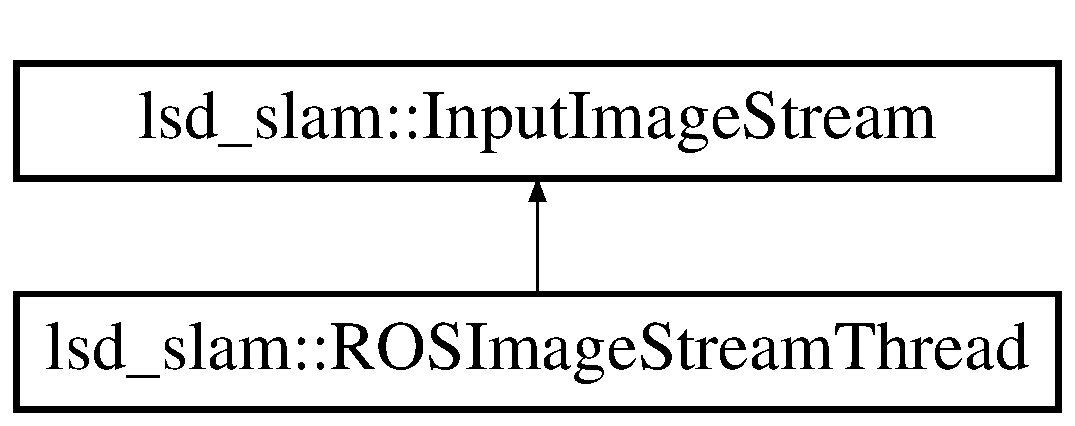
\includegraphics[height=2.000000cm]{classlsd__slam_1_1_input_image_stream}
\end{center}
\end{figure}
\subsection*{Public Member Functions}
\begin{DoxyCompactItemize}
\item 
virtual void \hyperlink{classlsd__slam_1_1_input_image_stream_a54d88ab343986e2a8f17d1ff5f5901be}{run} ()
\item 
\hypertarget{classlsd__slam_1_1_input_image_stream_a6e8bce6255dabfb4556e4fac8390a6b0}{virtual void {\bfseries set\-Calibration} (std\-::string file)}\label{classlsd__slam_1_1_input_image_stream_a6e8bce6255dabfb4556e4fac8390a6b0}

\item 
\hyperlink{classlsd__slam_1_1_notify_buffer}{Notify\-Buffer}$<$ \hyperlink{structlsd__slam_1_1_timestamped_object}{Timestamped\-Mat} $>$ $\ast$ \hyperlink{classlsd__slam_1_1_input_image_stream_ac8212a5168eb9bc3aa04f7bcc6922dfb}{get\-Buffer} ()
\item 
float \hyperlink{classlsd__slam_1_1_input_image_stream_a1198316d84d00116bcbee6358c591493}{fx} ()
\item 
\hypertarget{classlsd__slam_1_1_input_image_stream_ae8c6946d639eaa11bf228bb62fb0317c}{float {\bfseries fy} ()}\label{classlsd__slam_1_1_input_image_stream_ae8c6946d639eaa11bf228bb62fb0317c}

\item 
\hypertarget{classlsd__slam_1_1_input_image_stream_a56cdd46f70f734b5a3f34344f6f448ba}{float {\bfseries cx} ()}\label{classlsd__slam_1_1_input_image_stream_a56cdd46f70f734b5a3f34344f6f448ba}

\item 
\hypertarget{classlsd__slam_1_1_input_image_stream_a53b48fb8024b569ba167d886a2b28f3f}{float {\bfseries cy} ()}\label{classlsd__slam_1_1_input_image_stream_a53b48fb8024b569ba167d886a2b28f3f}

\item 
\hypertarget{classlsd__slam_1_1_input_image_stream_aae9c5e1689761e9ea6f9f4ce8682e8f1}{int {\bfseries width} ()}\label{classlsd__slam_1_1_input_image_stream_aae9c5e1689761e9ea6f9f4ce8682e8f1}

\item 
\hypertarget{classlsd__slam_1_1_input_image_stream_ab9a42e4ab63c80b7e0ba629ec689b7fa}{int {\bfseries height} ()}\label{classlsd__slam_1_1_input_image_stream_ab9a42e4ab63c80b7e0ba629ec689b7fa}

\end{DoxyCompactItemize}
\subsection*{Protected Attributes}
\begin{DoxyCompactItemize}
\item 
\hypertarget{classlsd__slam_1_1_input_image_stream_ad67ef5a34166c0cae737135a3c6e4375}{\hyperlink{classlsd__slam_1_1_notify_buffer}{Notify\-Buffer}$<$ \hyperlink{structlsd__slam_1_1_timestamped_object}{Timestamped\-Mat} $>$ $\ast$ {\bfseries image\-Buffer}}\label{classlsd__slam_1_1_input_image_stream_ad67ef5a34166c0cae737135a3c6e4375}

\item 
\hypertarget{classlsd__slam_1_1_input_image_stream_a2808cd73e1560f579da992f5eb45c451}{float {\bfseries fx\-\_\-}}\label{classlsd__slam_1_1_input_image_stream_a2808cd73e1560f579da992f5eb45c451}

\item 
\hypertarget{classlsd__slam_1_1_input_image_stream_abd686d1040fe5fcfb165c1a1ee8369d9}{float {\bfseries fy\-\_\-}}\label{classlsd__slam_1_1_input_image_stream_abd686d1040fe5fcfb165c1a1ee8369d9}

\item 
\hypertarget{classlsd__slam_1_1_input_image_stream_a9e93e4726bb40a37e1f23805703319bb}{float {\bfseries cx\-\_\-}}\label{classlsd__slam_1_1_input_image_stream_a9e93e4726bb40a37e1f23805703319bb}

\item 
\hypertarget{classlsd__slam_1_1_input_image_stream_aa7abd971928f3f58dd02a8e9e0eda804}{float {\bfseries cy\-\_\-}}\label{classlsd__slam_1_1_input_image_stream_aa7abd971928f3f58dd02a8e9e0eda804}

\item 
\hypertarget{classlsd__slam_1_1_input_image_stream_a9f0c3363cfc33682502b93b18324749c}{int {\bfseries width\-\_\-}}\label{classlsd__slam_1_1_input_image_stream_a9f0c3363cfc33682502b93b18324749c}

\item 
\hypertarget{classlsd__slam_1_1_input_image_stream_a58c25612f8ac94888c983bc3cffce39e}{int {\bfseries height\-\_\-}}\label{classlsd__slam_1_1_input_image_stream_a58c25612f8ac94888c983bc3cffce39e}

\end{DoxyCompactItemize}


\subsection{Detailed Description}
Virtual Image\-Stream. Can be from Open\-C\-V's Image\-Capture, R\-O\-S or Android. Also has to provide the camera calibration for that stream, as well as the respective undistorter object (if required). Runs in it's own thread, and has a \hyperlink{classlsd__slam_1_1_notify_buffer}{Notify\-Buffer}, in which received images are stored. 

\subsection{Member Function Documentation}
\hypertarget{classlsd__slam_1_1_input_image_stream_a1198316d84d00116bcbee6358c591493}{\index{lsd\-\_\-slam\-::\-Input\-Image\-Stream@{lsd\-\_\-slam\-::\-Input\-Image\-Stream}!fx@{fx}}
\index{fx@{fx}!lsd_slam::InputImageStream@{lsd\-\_\-slam\-::\-Input\-Image\-Stream}}
\subsubsection[{fx}]{\setlength{\rightskip}{0pt plus 5cm}float lsd\-\_\-slam\-::\-Input\-Image\-Stream\-::fx (
\begin{DoxyParamCaption}
{}
\end{DoxyParamCaption}
)\hspace{0.3cm}{\ttfamily [inline]}}}\label{classlsd__slam_1_1_input_image_stream_a1198316d84d00116bcbee6358c591493}
Gets the Camera Calibration. To avoid any dependencies, just as simple float / int's. \hypertarget{classlsd__slam_1_1_input_image_stream_ac8212a5168eb9bc3aa04f7bcc6922dfb}{\index{lsd\-\_\-slam\-::\-Input\-Image\-Stream@{lsd\-\_\-slam\-::\-Input\-Image\-Stream}!get\-Buffer@{get\-Buffer}}
\index{get\-Buffer@{get\-Buffer}!lsd_slam::InputImageStream@{lsd\-\_\-slam\-::\-Input\-Image\-Stream}}
\subsubsection[{get\-Buffer}]{\setlength{\rightskip}{0pt plus 5cm}{\bf Notify\-Buffer}$<${\bf Timestamped\-Mat}$>$$\ast$ lsd\-\_\-slam\-::\-Input\-Image\-Stream\-::get\-Buffer (
\begin{DoxyParamCaption}
{}
\end{DoxyParamCaption}
)\hspace{0.3cm}{\ttfamily [inline]}}}\label{classlsd__slam_1_1_input_image_stream_ac8212a5168eb9bc3aa04f7bcc6922dfb}
Gets the \hyperlink{classlsd__slam_1_1_notify_buffer}{Notify\-Buffer} to which incoming images are stored. \hypertarget{classlsd__slam_1_1_input_image_stream_a54d88ab343986e2a8f17d1ff5f5901be}{\index{lsd\-\_\-slam\-::\-Input\-Image\-Stream@{lsd\-\_\-slam\-::\-Input\-Image\-Stream}!run@{run}}
\index{run@{run}!lsd_slam::InputImageStream@{lsd\-\_\-slam\-::\-Input\-Image\-Stream}}
\subsubsection[{run}]{\setlength{\rightskip}{0pt plus 5cm}virtual void lsd\-\_\-slam\-::\-Input\-Image\-Stream\-::run (
\begin{DoxyParamCaption}
{}
\end{DoxyParamCaption}
)\hspace{0.3cm}{\ttfamily [inline]}, {\ttfamily [virtual]}}}\label{classlsd__slam_1_1_input_image_stream_a54d88ab343986e2a8f17d1ff5f5901be}
Starts the thread. 

Reimplemented in \hyperlink{classlsd__slam_1_1_r_o_s_image_stream_thread_a8d20574101837956cdebe14761c368fc}{lsd\-\_\-slam\-::\-R\-O\-S\-Image\-Stream\-Thread}.



The documentation for this class was generated from the following file\-:\begin{DoxyCompactItemize}
\item 
/home/king/rgbd-\/slam-\/lets-\/do-\/it/9-\/doxygen/lsd\-\_\-slam/lsd\-\_\-slam\-\_\-core/src/\-I\-O\-Wrapper/Input\-Image\-Stream.\-h\end{DoxyCompactItemize}

\hypertarget{structlsd__slam_1_1_input_point_dense}{\section{lsd\-\_\-slam\-:\-:Input\-Point\-Dense Struct Reference}
\label{structlsd__slam_1_1_input_point_dense}\index{lsd\-\_\-slam\-::\-Input\-Point\-Dense@{lsd\-\_\-slam\-::\-Input\-Point\-Dense}}
}
\subsection*{Public Attributes}
\begin{DoxyCompactItemize}
\item 
\hypertarget{structlsd__slam_1_1_input_point_dense_ad3277043db986bfcd8af8320ab36baad}{float {\bfseries idepth}}\label{structlsd__slam_1_1_input_point_dense_ad3277043db986bfcd8af8320ab36baad}

\item 
\hypertarget{structlsd__slam_1_1_input_point_dense_a105d1eb019fe8bb5fb4b2760e5f98f75}{float {\bfseries idepth\-\_\-var}}\label{structlsd__slam_1_1_input_point_dense_a105d1eb019fe8bb5fb4b2760e5f98f75}

\item 
\hypertarget{structlsd__slam_1_1_input_point_dense_ae85556d429ada57ea06a8a38ca5bca33}{unsigned char {\bfseries color} \mbox{[}4\mbox{]}}\label{structlsd__slam_1_1_input_point_dense_ae85556d429ada57ea06a8a38ca5bca33}

\end{DoxyCompactItemize}


The documentation for this struct was generated from the following file\-:\begin{DoxyCompactItemize}
\item 
/home/king/rgbd-\/slam-\/lets-\/do-\/it/9-\/doxygen/lsd\-\_\-slam/lsd\-\_\-slam\-\_\-core/src/\-I\-O\-Wrapper/\-R\-O\-S/R\-O\-S\-Output3\-D\-Wrapper.\-h\end{DoxyCompactItemize}

\hypertarget{classlsd__slam_1_1_key_frame_graph}{\section{lsd\-\_\-slam\-:\-:Key\-Frame\-Graph Class Reference}
\label{classlsd__slam_1_1_key_frame_graph}\index{lsd\-\_\-slam\-::\-Key\-Frame\-Graph@{lsd\-\_\-slam\-::\-Key\-Frame\-Graph}}
}


{\ttfamily \#include $<$Key\-Frame\-Graph.\-h$>$}

\subsection*{Public Member Functions}
\begin{DoxyCompactItemize}
\item 
E\-I\-G\-E\-N\-\_\-\-M\-A\-K\-E\-\_\-\-A\-L\-I\-G\-N\-E\-D\-\_\-\-O\-P\-E\-R\-A\-T\-O\-R\-\_\-\-N\-E\-W \hyperlink{classlsd__slam_1_1_key_frame_graph_a998e4c0fe64cb8f8aa59163cc68bf176}{Key\-Frame\-Graph} ()
\item 
\hyperlink{classlsd__slam_1_1_key_frame_graph_a0fb3ba7d0f694dce13c9da32a47f09fd}{$\sim$\-Key\-Frame\-Graph} ()
\item 
void \hyperlink{classlsd__slam_1_1_key_frame_graph_a3a8b7205a3f3e8702bf4c74abd7fccf5}{add\-Key\-Frame} (\hyperlink{classlsd__slam_1_1_frame}{Frame} $\ast$frame)
\item 
void \hyperlink{classlsd__slam_1_1_key_frame_graph_a5e04ab1456118e86090ae4baa736c0d5}{add\-Frame} (\hyperlink{classlsd__slam_1_1_frame}{Frame} $\ast$frame)
\item 
\hypertarget{classlsd__slam_1_1_key_frame_graph_a02a50466a5ff143c8e68cbca1a495efe}{void {\bfseries dump\-Map} (std\-::string folder)}\label{classlsd__slam_1_1_key_frame_graph_a02a50466a5ff143c8e68cbca1a495efe}

\item 
void \hyperlink{classlsd__slam_1_1_key_frame_graph_a0e4cf71471fcea9fc3aa5fab8c3aa2a3}{insert\-Constraint} (\hyperlink{structlsd__slam_1_1_k_f_constraint_struct}{K\-F\-Constraint\-Struct} $\ast$constraint)
\item 
int \hyperlink{classlsd__slam_1_1_key_frame_graph_a222149dbc9f7a35bb5e97d6aa6580b14}{optimize} (int num\-\_\-iterations)
\item 
\hypertarget{classlsd__slam_1_1_key_frame_graph_aa99125c2838d861bf5737ee9b9568d89}{bool {\bfseries add\-Elements\-From\-Buffer} ()}\label{classlsd__slam_1_1_key_frame_graph_aa99125c2838d861bf5737ee9b9568d89}

\item 
void \hyperlink{classlsd__slam_1_1_key_frame_graph_a01cb0488a64d79a500265d9096b6a014}{calculate\-Graph\-Distances\-To\-Frame} (\hyperlink{classlsd__slam_1_1_frame}{Frame} $\ast$frame, std\-::unordered\-\_\-map$<$ \hyperlink{classlsd__slam_1_1_frame}{Frame} $\ast$, int $>$ $\ast$distance\-Map)
\end{DoxyCompactItemize}
\subsection*{Public Attributes}
\begin{DoxyCompactItemize}
\item 
\hypertarget{classlsd__slam_1_1_key_frame_graph_a8ec7de131b7f76f8ec2e39a61749df2c}{int {\bfseries total\-Points}}\label{classlsd__slam_1_1_key_frame_graph_a8ec7de131b7f76f8ec2e39a61749df2c}

\item 
\hypertarget{classlsd__slam_1_1_key_frame_graph_a8748ec0a5f59cf2ce97897564bf33cae}{int {\bfseries total\-Edges}}\label{classlsd__slam_1_1_key_frame_graph_a8748ec0a5f59cf2ce97897564bf33cae}

\item 
\hypertarget{classlsd__slam_1_1_key_frame_graph_aac32e1096f7100dd4d53f362a72d274c}{int {\bfseries total\-Vertices}}\label{classlsd__slam_1_1_key_frame_graph_aac32e1096f7100dd4d53f362a72d274c}

\item 
\hypertarget{classlsd__slam_1_1_key_frame_graph_a83c40c8d72058ddc99962be77f53e4a6}{boost\-::shared\-\_\-mutex {\bfseries keyframes\-All\-Mutex}}\label{classlsd__slam_1_1_key_frame_graph_a83c40c8d72058ddc99962be77f53e4a6}

\item 
\hypertarget{classlsd__slam_1_1_key_frame_graph_a7af6ef4d5240a03c7871f64ab96c67cc}{std\-::vector$<$ \hyperlink{classlsd__slam_1_1_frame}{Frame} \\*
$\ast$, Eigen\-::aligned\-\_\-allocator\\*
$<$ \hyperlink{classlsd__slam_1_1_frame}{Frame} $\ast$ $>$ $>$ {\bfseries keyframes\-All}}\label{classlsd__slam_1_1_key_frame_graph_a7af6ef4d5240a03c7871f64ab96c67cc}

\item 
boost\-::shared\-\_\-mutex \hyperlink{classlsd__slam_1_1_key_frame_graph_aec658110a47437fdf2aa9c2fe2a074b4}{id\-To\-Key\-Frame\-Mutex}
\item 
\hypertarget{classlsd__slam_1_1_key_frame_graph_a478514f46156cc94b4fdc2479fa2323c}{std\-::unordered\-\_\-map$<$ int, \\*
std\-::shared\-\_\-ptr$<$ \hyperlink{classlsd__slam_1_1_frame}{Frame} $>$\\*
, std\-::hash$<$ int $>$\\*
, std\-::equal\-\_\-to$<$ int $>$\\*
, Eigen\-::aligned\-\_\-allocator\\*
$<$ std\-::pair$<$ const int, \\*
std\-::shared\-\_\-ptr$<$ \hyperlink{classlsd__slam_1_1_frame}{Frame} $>$ $>$ $>$ $>$ {\bfseries id\-To\-Key\-Frame}}\label{classlsd__slam_1_1_key_frame_graph_a478514f46156cc94b4fdc2479fa2323c}

\item 
\hypertarget{classlsd__slam_1_1_key_frame_graph_a3fcdb72f14397979e235c2e9ee2112ed}{boost\-::shared\-\_\-mutex {\bfseries edges\-Lists\-Mutex}}\label{classlsd__slam_1_1_key_frame_graph_a3fcdb72f14397979e235c2e9ee2112ed}

\item 
\hypertarget{classlsd__slam_1_1_key_frame_graph_a980d0a66a121b0616b273b5324a0c37e}{std\-::vector\\*
$<$ \hyperlink{structlsd__slam_1_1_k_f_constraint_struct}{K\-F\-Constraint\-Struct} \\*
$\ast$, Eigen\-::aligned\-\_\-allocator\\*
$<$ \hyperlink{structlsd__slam_1_1_k_f_constraint_struct}{K\-F\-Constraint\-Struct} $\ast$ $>$ $>$ {\bfseries edges\-All}}\label{classlsd__slam_1_1_key_frame_graph_a980d0a66a121b0616b273b5324a0c37e}

\item 
\hypertarget{classlsd__slam_1_1_key_frame_graph_a4cefb6b0075686d087b819a8458cce16}{boost\-::shared\-\_\-mutex {\bfseries all\-Frame\-Poses\-Mutex}}\label{classlsd__slam_1_1_key_frame_graph_a4cefb6b0075686d087b819a8458cce16}

\item 
\hypertarget{classlsd__slam_1_1_key_frame_graph_a9fe24ef732e68d2cc21efddcdf05e5ee}{std\-::vector$<$ \hyperlink{classlsd__slam_1_1_frame_pose_struct}{Frame\-Pose\-Struct} \\*
$\ast$, Eigen\-::aligned\-\_\-allocator\\*
$<$ \hyperlink{classlsd__slam_1_1_frame_pose_struct}{Frame\-Pose\-Struct} $\ast$ $>$ $>$ {\bfseries all\-Frame\-Poses}}\label{classlsd__slam_1_1_key_frame_graph_a9fe24ef732e68d2cc21efddcdf05e5ee}

\item 
\hypertarget{classlsd__slam_1_1_key_frame_graph_a0d165eb656f77b3737066a4cb855309b}{boost\-::mutex {\bfseries keyframes\-For\-Retrack\-Mutex}}\label{classlsd__slam_1_1_key_frame_graph_a0d165eb656f77b3737066a4cb855309b}

\item 
\hypertarget{classlsd__slam_1_1_key_frame_graph_a4c9313e998900b25bc1f1e090f0b1080}{std\-::deque$<$ \hyperlink{classlsd__slam_1_1_frame}{Frame} $\ast$ $>$ {\bfseries keyframes\-For\-Retrack}}\label{classlsd__slam_1_1_key_frame_graph_a4c9313e998900b25bc1f1e090f0b1080}

\end{DoxyCompactItemize}
\subsection*{Friends}
\begin{DoxyCompactItemize}
\item 
\hypertarget{classlsd__slam_1_1_key_frame_graph_a58b23779ede944b1716e0ffd20b379ae}{class {\bfseries Integration\-Test}}\label{classlsd__slam_1_1_key_frame_graph_a58b23779ede944b1716e0ffd20b379ae}

\end{DoxyCompactItemize}


\subsection{Detailed Description}
Graph consisting of Key\-Frames and constraints, performing optimization. 

\subsection{Constructor \& Destructor Documentation}
\hypertarget{classlsd__slam_1_1_key_frame_graph_a998e4c0fe64cb8f8aa59163cc68bf176}{\index{lsd\-\_\-slam\-::\-Key\-Frame\-Graph@{lsd\-\_\-slam\-::\-Key\-Frame\-Graph}!Key\-Frame\-Graph@{Key\-Frame\-Graph}}
\index{Key\-Frame\-Graph@{Key\-Frame\-Graph}!lsd_slam::KeyFrameGraph@{lsd\-\_\-slam\-::\-Key\-Frame\-Graph}}
\subsubsection[{Key\-Frame\-Graph}]{\setlength{\rightskip}{0pt plus 5cm}lsd\-\_\-slam\-::\-Key\-Frame\-Graph\-::\-Key\-Frame\-Graph (
\begin{DoxyParamCaption}
{}
\end{DoxyParamCaption}
)}}\label{classlsd__slam_1_1_key_frame_graph_a998e4c0fe64cb8f8aa59163cc68bf176}
Constructs an empty pose graph. \hypertarget{classlsd__slam_1_1_key_frame_graph_a0fb3ba7d0f694dce13c9da32a47f09fd}{\index{lsd\-\_\-slam\-::\-Key\-Frame\-Graph@{lsd\-\_\-slam\-::\-Key\-Frame\-Graph}!$\sim$\-Key\-Frame\-Graph@{$\sim$\-Key\-Frame\-Graph}}
\index{$\sim$\-Key\-Frame\-Graph@{$\sim$\-Key\-Frame\-Graph}!lsd_slam::KeyFrameGraph@{lsd\-\_\-slam\-::\-Key\-Frame\-Graph}}
\subsubsection[{$\sim$\-Key\-Frame\-Graph}]{\setlength{\rightskip}{0pt plus 5cm}lsd\-\_\-slam\-::\-Key\-Frame\-Graph\-::$\sim$\-Key\-Frame\-Graph (
\begin{DoxyParamCaption}
{}
\end{DoxyParamCaption}
)}}\label{classlsd__slam_1_1_key_frame_graph_a0fb3ba7d0f694dce13c9da32a47f09fd}
Deletes the g2o graph. 

\subsection{Member Function Documentation}
\hypertarget{classlsd__slam_1_1_key_frame_graph_a5e04ab1456118e86090ae4baa736c0d5}{\index{lsd\-\_\-slam\-::\-Key\-Frame\-Graph@{lsd\-\_\-slam\-::\-Key\-Frame\-Graph}!add\-Frame@{add\-Frame}}
\index{add\-Frame@{add\-Frame}!lsd_slam::KeyFrameGraph@{lsd\-\_\-slam\-::\-Key\-Frame\-Graph}}
\subsubsection[{add\-Frame}]{\setlength{\rightskip}{0pt plus 5cm}void lsd\-\_\-slam\-::\-Key\-Frame\-Graph\-::add\-Frame (
\begin{DoxyParamCaption}
\item[{{\bf Frame} $\ast$}]{frame}
\end{DoxyParamCaption}
)}}\label{classlsd__slam_1_1_key_frame_graph_a5e04ab1456118e86090ae4baa736c0d5}
Adds a new \hyperlink{classlsd__slam_1_1_frame}{Frame} to the graph. Doesnt actually keep the frame, but only it's pose-\/struct. \hypertarget{classlsd__slam_1_1_key_frame_graph_a3a8b7205a3f3e8702bf4c74abd7fccf5}{\index{lsd\-\_\-slam\-::\-Key\-Frame\-Graph@{lsd\-\_\-slam\-::\-Key\-Frame\-Graph}!add\-Key\-Frame@{add\-Key\-Frame}}
\index{add\-Key\-Frame@{add\-Key\-Frame}!lsd_slam::KeyFrameGraph@{lsd\-\_\-slam\-::\-Key\-Frame\-Graph}}
\subsubsection[{add\-Key\-Frame}]{\setlength{\rightskip}{0pt plus 5cm}void lsd\-\_\-slam\-::\-Key\-Frame\-Graph\-::add\-Key\-Frame (
\begin{DoxyParamCaption}
\item[{{\bf Frame} $\ast$}]{frame}
\end{DoxyParamCaption}
)}}\label{classlsd__slam_1_1_key_frame_graph_a3a8b7205a3f3e8702bf4c74abd7fccf5}
Adds a new Key\-Frame to the graph. \hypertarget{classlsd__slam_1_1_key_frame_graph_a01cb0488a64d79a500265d9096b6a014}{\index{lsd\-\_\-slam\-::\-Key\-Frame\-Graph@{lsd\-\_\-slam\-::\-Key\-Frame\-Graph}!calculate\-Graph\-Distances\-To\-Frame@{calculate\-Graph\-Distances\-To\-Frame}}
\index{calculate\-Graph\-Distances\-To\-Frame@{calculate\-Graph\-Distances\-To\-Frame}!lsd_slam::KeyFrameGraph@{lsd\-\_\-slam\-::\-Key\-Frame\-Graph}}
\subsubsection[{calculate\-Graph\-Distances\-To\-Frame}]{\setlength{\rightskip}{0pt plus 5cm}void lsd\-\_\-slam\-::\-Key\-Frame\-Graph\-::calculate\-Graph\-Distances\-To\-Frame (
\begin{DoxyParamCaption}
\item[{{\bf Frame} $\ast$}]{frame, }
\item[{std\-::unordered\-\_\-map$<$ {\bf Frame} $\ast$, int $>$ $\ast$}]{distance\-Map}
\end{DoxyParamCaption}
)}}\label{classlsd__slam_1_1_key_frame_graph_a01cb0488a64d79a500265d9096b6a014}
Creates a hash map of keyframe -\/$>$ distance to given frame. \hypertarget{classlsd__slam_1_1_key_frame_graph_a0e4cf71471fcea9fc3aa5fab8c3aa2a3}{\index{lsd\-\_\-slam\-::\-Key\-Frame\-Graph@{lsd\-\_\-slam\-::\-Key\-Frame\-Graph}!insert\-Constraint@{insert\-Constraint}}
\index{insert\-Constraint@{insert\-Constraint}!lsd_slam::KeyFrameGraph@{lsd\-\_\-slam\-::\-Key\-Frame\-Graph}}
\subsubsection[{insert\-Constraint}]{\setlength{\rightskip}{0pt plus 5cm}void lsd\-\_\-slam\-::\-Key\-Frame\-Graph\-::insert\-Constraint (
\begin{DoxyParamCaption}
\item[{{\bf K\-F\-Constraint\-Struct} $\ast$}]{constraint}
\end{DoxyParamCaption}
)}}\label{classlsd__slam_1_1_key_frame_graph_a0e4cf71471fcea9fc3aa5fab8c3aa2a3}
Adds a new constraint to the graph.

The transformation must map world points such that they move as if attached to a frame which moves from first\-Frame to second\-Frame\-: second-\/$>$cam\-To\-World $\ast$ first-\/$>$world\-To\-Cam $\ast$ point

If is\-Odometry\-Constraint is set, scale\-Information is ignored. \hypertarget{classlsd__slam_1_1_key_frame_graph_a222149dbc9f7a35bb5e97d6aa6580b14}{\index{lsd\-\_\-slam\-::\-Key\-Frame\-Graph@{lsd\-\_\-slam\-::\-Key\-Frame\-Graph}!optimize@{optimize}}
\index{optimize@{optimize}!lsd_slam::KeyFrameGraph@{lsd\-\_\-slam\-::\-Key\-Frame\-Graph}}
\subsubsection[{optimize}]{\setlength{\rightskip}{0pt plus 5cm}int lsd\-\_\-slam\-::\-Key\-Frame\-Graph\-::optimize (
\begin{DoxyParamCaption}
\item[{int}]{num\-\_\-iterations}
\end{DoxyParamCaption}
)}}\label{classlsd__slam_1_1_key_frame_graph_a222149dbc9f7a35bb5e97d6aa6580b14}
Optimizes the graph. Does not update the keyframe poses, only the vertex poses. You must call update\-Key\-Frame\-Poses() afterwards. 

\subsection{Member Data Documentation}
\hypertarget{classlsd__slam_1_1_key_frame_graph_aec658110a47437fdf2aa9c2fe2a074b4}{\index{lsd\-\_\-slam\-::\-Key\-Frame\-Graph@{lsd\-\_\-slam\-::\-Key\-Frame\-Graph}!id\-To\-Key\-Frame\-Mutex@{id\-To\-Key\-Frame\-Mutex}}
\index{id\-To\-Key\-Frame\-Mutex@{id\-To\-Key\-Frame\-Mutex}!lsd_slam::KeyFrameGraph@{lsd\-\_\-slam\-::\-Key\-Frame\-Graph}}
\subsubsection[{id\-To\-Key\-Frame\-Mutex}]{\setlength{\rightskip}{0pt plus 5cm}boost\-::shared\-\_\-mutex lsd\-\_\-slam\-::\-Key\-Frame\-Graph\-::id\-To\-Key\-Frame\-Mutex}}\label{classlsd__slam_1_1_key_frame_graph_aec658110a47437fdf2aa9c2fe2a074b4}
Maps frame ids to keyframes. Contains A\-L\-L Keyframes allocated, including the one that currently being created. 

The documentation for this class was generated from the following files\-:\begin{DoxyCompactItemize}
\item 
/home/king/rgbd-\/slam-\/lets-\/do-\/it/9-\/doxygen/lsd\-\_\-slam/lsd\-\_\-slam\-\_\-core/src/\-Global\-Mapping/Key\-Frame\-Graph.\-h\item 
/home/king/rgbd-\/slam-\/lets-\/do-\/it/9-\/doxygen/lsd\-\_\-slam/lsd\-\_\-slam\-\_\-core/src/\-Global\-Mapping/Key\-Frame\-Graph.\-cpp\end{DoxyCompactItemize}

\hypertarget{structlsd__slam_1_1_k_f_constraint_struct}{\section{lsd\-\_\-slam\-:\-:K\-F\-Constraint\-Struct Struct Reference}
\label{structlsd__slam_1_1_k_f_constraint_struct}\index{lsd\-\_\-slam\-::\-K\-F\-Constraint\-Struct@{lsd\-\_\-slam\-::\-K\-F\-Constraint\-Struct}}
}
\subsection*{Public Attributes}
\begin{DoxyCompactItemize}
\item 
\hypertarget{structlsd__slam_1_1_k_f_constraint_struct_a8f0cce58b7893cfc20db26e0e0390973}{\hyperlink{classlsd__slam_1_1_frame}{Frame} $\ast$ {\bfseries first\-Frame}}\label{structlsd__slam_1_1_k_f_constraint_struct_a8f0cce58b7893cfc20db26e0e0390973}

\item 
\hypertarget{structlsd__slam_1_1_k_f_constraint_struct_aa98538143de8fedbf6f9d0f911c897f0}{\hyperlink{classlsd__slam_1_1_frame}{Frame} $\ast$ {\bfseries second\-Frame}}\label{structlsd__slam_1_1_k_f_constraint_struct_aa98538143de8fedbf6f9d0f911c897f0}

\item 
\hypertarget{structlsd__slam_1_1_k_f_constraint_struct_af270b4ccf00a399edb46d22212d3742c}{Sophus\-::\-Sim3d {\bfseries second\-To\-First}}\label{structlsd__slam_1_1_k_f_constraint_struct_af270b4ccf00a399edb46d22212d3742c}

\item 
\hypertarget{structlsd__slam_1_1_k_f_constraint_struct_ac5d4ed69143845a556a648753c3188a2}{Eigen\-::\-Matrix$<$ double, 7, 7 $>$ {\bfseries information}}\label{structlsd__slam_1_1_k_f_constraint_struct_ac5d4ed69143845a556a648753c3188a2}

\item 
\hypertarget{structlsd__slam_1_1_k_f_constraint_struct_a38bff9ba91ca70d2bfdd34492ea4dd5d}{g2o\-::\-Robust\-Kernel $\ast$ {\bfseries robust\-Kernel}}\label{structlsd__slam_1_1_k_f_constraint_struct_a38bff9ba91ca70d2bfdd34492ea4dd5d}

\item 
\hypertarget{structlsd__slam_1_1_k_f_constraint_struct_a0f01605816cb3ae6c5ec8272ca84cf29}{\hyperlink{classlsd__slam_1_1_edge_sim3}{Edge\-Sim3} $\ast$ {\bfseries edge}}\label{structlsd__slam_1_1_k_f_constraint_struct_a0f01605816cb3ae6c5ec8272ca84cf29}

\item 
\hypertarget{structlsd__slam_1_1_k_f_constraint_struct_a4733c48b4b01efa316fe343983079b36}{float {\bfseries usage}}\label{structlsd__slam_1_1_k_f_constraint_struct_a4733c48b4b01efa316fe343983079b36}

\item 
\hypertarget{structlsd__slam_1_1_k_f_constraint_struct_a56d3514b0a01ff5968a9b1a5ccc1beaf}{float {\bfseries mean\-Residual\-D}}\label{structlsd__slam_1_1_k_f_constraint_struct_a56d3514b0a01ff5968a9b1a5ccc1beaf}

\item 
\hypertarget{structlsd__slam_1_1_k_f_constraint_struct_a68a32baf3e42ba069b601a4556438d98}{float {\bfseries mean\-Residual\-P}}\label{structlsd__slam_1_1_k_f_constraint_struct_a68a32baf3e42ba069b601a4556438d98}

\item 
\hypertarget{structlsd__slam_1_1_k_f_constraint_struct_acd1814fc35a44c58779184f2950e7658}{float {\bfseries mean\-Residual}}\label{structlsd__slam_1_1_k_f_constraint_struct_acd1814fc35a44c58779184f2950e7658}

\item 
\hypertarget{structlsd__slam_1_1_k_f_constraint_struct_ab34a87d36118a5d15d4c88a0f280ce86}{float {\bfseries reciprocal\-Consistency}}\label{structlsd__slam_1_1_k_f_constraint_struct_ab34a87d36118a5d15d4c88a0f280ce86}

\item 
\hypertarget{structlsd__slam_1_1_k_f_constraint_struct_ab8e306aca770595b3ab5dc6cb84f53c5}{int {\bfseries idx\-In\-All\-Edges}}\label{structlsd__slam_1_1_k_f_constraint_struct_ab8e306aca770595b3ab5dc6cb84f53c5}

\end{DoxyCompactItemize}


The documentation for this struct was generated from the following files\-:\begin{DoxyCompactItemize}
\item 
/home/king/rgbd-\/slam-\/lets-\/do-\/it/9-\/doxygen/lsd\-\_\-slam/lsd\-\_\-slam\-\_\-core/src/\-Global\-Mapping/Key\-Frame\-Graph.\-h\item 
/home/king/rgbd-\/slam-\/lets-\/do-\/it/9-\/doxygen/lsd\-\_\-slam/lsd\-\_\-slam\-\_\-core/src/\-Global\-Mapping/Key\-Frame\-Graph.\-cpp\end{DoxyCompactItemize}

\hypertarget{classlsd__slam_1_1_l_g_s4}{\section{lsd\-\_\-slam\-:\-:L\-G\-S4 Class Reference}
\label{classlsd__slam_1_1_l_g_s4}\index{lsd\-\_\-slam\-::\-L\-G\-S4@{lsd\-\_\-slam\-::\-L\-G\-S4}}
}
\subsection*{Public Member Functions}
\begin{DoxyCompactItemize}
\item 
\hypertarget{classlsd__slam_1_1_l_g_s4_aa18a8ed78f76874149cfdc2cb04820f0}{void {\bfseries initialize} (const size\-\_\-t maxnum\-\_\-constraints)}\label{classlsd__slam_1_1_l_g_s4_aa18a8ed78f76874149cfdc2cb04820f0}

\item 
\hypertarget{classlsd__slam_1_1_l_g_s4_ab730fee0bb7add5743440ea1551b6fa8}{void {\bfseries finish\-No\-Divide} ()}\label{classlsd__slam_1_1_l_g_s4_ab730fee0bb7add5743440ea1551b6fa8}

\item 
\hypertarget{classlsd__slam_1_1_l_g_s4_adbc23aff94e3bcc39132e6f351f12187}{void {\bfseries update} (const Vector4 \&J, const float \&res, const float \&weight)}\label{classlsd__slam_1_1_l_g_s4_adbc23aff94e3bcc39132e6f351f12187}

\end{DoxyCompactItemize}
\subsection*{Public Attributes}
\begin{DoxyCompactItemize}
\item 
\hypertarget{classlsd__slam_1_1_l_g_s4_a82f7fa9153f1ebd8eff2a04944a79bbc}{{\bfseries E\-I\-G\-E\-N\-\_\-\-M\-A\-K\-E\-\_\-\-A\-L\-I\-G\-N\-E\-D\-\_\-\-O\-P\-E\-R\-A\-T\-O\-R\-\_\-\-N\-E\-W}}\label{classlsd__slam_1_1_l_g_s4_a82f7fa9153f1ebd8eff2a04944a79bbc}

\item 
\hypertarget{classlsd__slam_1_1_l_g_s4_a0d77b03bd67cc028911e06ebf4ad1ddb}{Matrix4x4 {\bfseries A}}\label{classlsd__slam_1_1_l_g_s4_a0d77b03bd67cc028911e06ebf4ad1ddb}

\item 
\hypertarget{classlsd__slam_1_1_l_g_s4_a1ea8e55e9d4d9a2abad2155d6681685d}{Vector4 {\bfseries b}}\label{classlsd__slam_1_1_l_g_s4_a1ea8e55e9d4d9a2abad2155d6681685d}

\item 
\hypertarget{classlsd__slam_1_1_l_g_s4_a0d55f3863b9517c364012b8fa10e1ffe}{float {\bfseries error}}\label{classlsd__slam_1_1_l_g_s4_a0d55f3863b9517c364012b8fa10e1ffe}

\item 
\hypertarget{classlsd__slam_1_1_l_g_s4_a7b58033ce0401ab287d40e9a0ce6f6ed}{size\-\_\-t {\bfseries num\-\_\-constraints}}\label{classlsd__slam_1_1_l_g_s4_a7b58033ce0401ab287d40e9a0ce6f6ed}

\end{DoxyCompactItemize}


The documentation for this class was generated from the following file\-:\begin{DoxyCompactItemize}
\item 
/home/king/rgbd-\/slam-\/lets-\/do-\/it/9-\/doxygen/lsd\-\_\-slam/lsd\-\_\-slam\-\_\-core/src/\-Tracking/L\-G\-S\-X.\-h\end{DoxyCompactItemize}

\hypertarget{classlsd__slam_1_1_l_g_s6}{\section{lsd\-\_\-slam\-:\-:L\-G\-S6 Class Reference}
\label{classlsd__slam_1_1_l_g_s6}\index{lsd\-\_\-slam\-::\-L\-G\-S6@{lsd\-\_\-slam\-::\-L\-G\-S6}}
}


{\ttfamily \#include $<$L\-G\-S\-X.\-h$>$}

\subsection*{Public Member Functions}
\begin{DoxyCompactItemize}
\item 
\hypertarget{classlsd__slam_1_1_l_g_s6_a91e91981c8eb3771922f0d350be07b1c}{void {\bfseries initialize} (const size\-\_\-t maxnum\-\_\-constraints)}\label{classlsd__slam_1_1_l_g_s6_a91e91981c8eb3771922f0d350be07b1c}

\item 
\hypertarget{classlsd__slam_1_1_l_g_s6_a174aafb481a9203f29f4201aaa80a4bc}{void {\bfseries finish\-No\-Divide} ()}\label{classlsd__slam_1_1_l_g_s6_a174aafb481a9203f29f4201aaa80a4bc}

\item 
\hypertarget{classlsd__slam_1_1_l_g_s6_a54942513c8e6a2a252770019bc1e8ebc}{void {\bfseries finish} ()}\label{classlsd__slam_1_1_l_g_s6_a54942513c8e6a2a252770019bc1e8ebc}

\item 
\hypertarget{classlsd__slam_1_1_l_g_s6_a386ed7b47af111f1aed1182f63c0c846}{void {\bfseries update} (const Vector6 \&J, const float \&res, const float \&weight)}\label{classlsd__slam_1_1_l_g_s6_a386ed7b47af111f1aed1182f63c0c846}

\end{DoxyCompactItemize}
\subsection*{Public Attributes}
\begin{DoxyCompactItemize}
\item 
\hypertarget{classlsd__slam_1_1_l_g_s6_a0c72470af8948ecb5b0d7e9ff5a1c5bc}{{\bfseries E\-I\-G\-E\-N\-\_\-\-M\-A\-K\-E\-\_\-\-A\-L\-I\-G\-N\-E\-D\-\_\-\-O\-P\-E\-R\-A\-T\-O\-R\-\_\-\-N\-E\-W}}\label{classlsd__slam_1_1_l_g_s6_a0c72470af8948ecb5b0d7e9ff5a1c5bc}

\item 
\hypertarget{classlsd__slam_1_1_l_g_s6_a2d14c1a984450273bb01a0941fbf5ada}{Matrix6x6 {\bfseries A}}\label{classlsd__slam_1_1_l_g_s6_a2d14c1a984450273bb01a0941fbf5ada}

\item 
\hypertarget{classlsd__slam_1_1_l_g_s6_ad3613ae9cd1f502695d732b6d9b13365}{Vector6 {\bfseries b}}\label{classlsd__slam_1_1_l_g_s6_ad3613ae9cd1f502695d732b6d9b13365}

\item 
\hypertarget{classlsd__slam_1_1_l_g_s6_ae623a9c4889b5d0be7da81c809c3938c}{float {\bfseries error}}\label{classlsd__slam_1_1_l_g_s6_ae623a9c4889b5d0be7da81c809c3938c}

\item 
\hypertarget{classlsd__slam_1_1_l_g_s6_a354b8d5d6d95cdd517c5e749581d14cf}{size\-\_\-t {\bfseries num\-\_\-constraints}}\label{classlsd__slam_1_1_l_g_s6_a354b8d5d6d95cdd517c5e749581d14cf}

\end{DoxyCompactItemize}


\subsection{Detailed Description}
Builds 4dof L\-G\-S (used for depth-\/lgs, at it has only 7 non-\/zero entries in jacobian) only used to accumulate data, N\-O\-T really as L\-G\-S 

The documentation for this class was generated from the following file\-:\begin{DoxyCompactItemize}
\item 
/home/king/rgbd-\/slam-\/lets-\/do-\/it/9-\/doxygen/lsd\-\_\-slam/lsd\-\_\-slam\-\_\-core/src/\-Tracking/L\-G\-S\-X.\-h\end{DoxyCompactItemize}

\hypertarget{classlsd__slam_1_1_l_g_s7}{\section{lsd\-\_\-slam\-:\-:L\-G\-S7 Class Reference}
\label{classlsd__slam_1_1_l_g_s7}\index{lsd\-\_\-slam\-::\-L\-G\-S7@{lsd\-\_\-slam\-::\-L\-G\-S7}}
}
\subsection*{Public Member Functions}
\begin{DoxyCompactItemize}
\item 
\hypertarget{classlsd__slam_1_1_l_g_s7_af21bdd9bdbd7997725fe4c1da809e437}{void {\bfseries initialize\-From} (const \hyperlink{classlsd__slam_1_1_l_g_s6}{L\-G\-S6} \&ls6, const \hyperlink{classlsd__slam_1_1_l_g_s4}{L\-G\-S4} \&ls4)}\label{classlsd__slam_1_1_l_g_s7_af21bdd9bdbd7997725fe4c1da809e437}

\end{DoxyCompactItemize}
\subsection*{Public Attributes}
\begin{DoxyCompactItemize}
\item 
\hypertarget{classlsd__slam_1_1_l_g_s7_a047aa7711a2a7276ad380dac78d63ca2}{{\bfseries E\-I\-G\-E\-N\-\_\-\-M\-A\-K\-E\-\_\-\-A\-L\-I\-G\-N\-E\-D\-\_\-\-O\-P\-E\-R\-A\-T\-O\-R\-\_\-\-N\-E\-W}}\label{classlsd__slam_1_1_l_g_s7_a047aa7711a2a7276ad380dac78d63ca2}

\item 
\hypertarget{classlsd__slam_1_1_l_g_s7_aa421de346f4eff019fc35b08560094b0}{Matrix7x7 {\bfseries A}}\label{classlsd__slam_1_1_l_g_s7_aa421de346f4eff019fc35b08560094b0}

\item 
\hypertarget{classlsd__slam_1_1_l_g_s7_a1a52d3afe19079476e89f1d46e0d823c}{Vector7 {\bfseries b}}\label{classlsd__slam_1_1_l_g_s7_a1a52d3afe19079476e89f1d46e0d823c}

\item 
\hypertarget{classlsd__slam_1_1_l_g_s7_ab9569f227f26c8e1d083ddcb4cd59e7d}{float {\bfseries error}}\label{classlsd__slam_1_1_l_g_s7_ab9569f227f26c8e1d083ddcb4cd59e7d}

\item 
\hypertarget{classlsd__slam_1_1_l_g_s7_a9a8103f356a42d715c7aff24c45c54de}{size\-\_\-t {\bfseries num\-\_\-constraints}}\label{classlsd__slam_1_1_l_g_s7_a9a8103f356a42d715c7aff24c45c54de}

\end{DoxyCompactItemize}


The documentation for this class was generated from the following file\-:\begin{DoxyCompactItemize}
\item 
/home/king/rgbd-\/slam-\/lets-\/do-\/it/9-\/doxygen/lsd\-\_\-slam/lsd\-\_\-slam\-\_\-core/src/\-Tracking/L\-G\-S\-X.\-h\end{DoxyCompactItemize}

\hypertarget{structlsd__slam_1_1_live_s_l_a_m_wrapper}{\section{lsd\-\_\-slam\-:\-:Live\-S\-L\-A\-M\-Wrapper Struct Reference}
\label{structlsd__slam_1_1_live_s_l_a_m_wrapper}\index{lsd\-\_\-slam\-::\-Live\-S\-L\-A\-M\-Wrapper@{lsd\-\_\-slam\-::\-Live\-S\-L\-A\-M\-Wrapper}}
}
Inheritance diagram for lsd\-\_\-slam\-:\-:Live\-S\-L\-A\-M\-Wrapper\-:\begin{figure}[H]
\begin{center}
\leavevmode
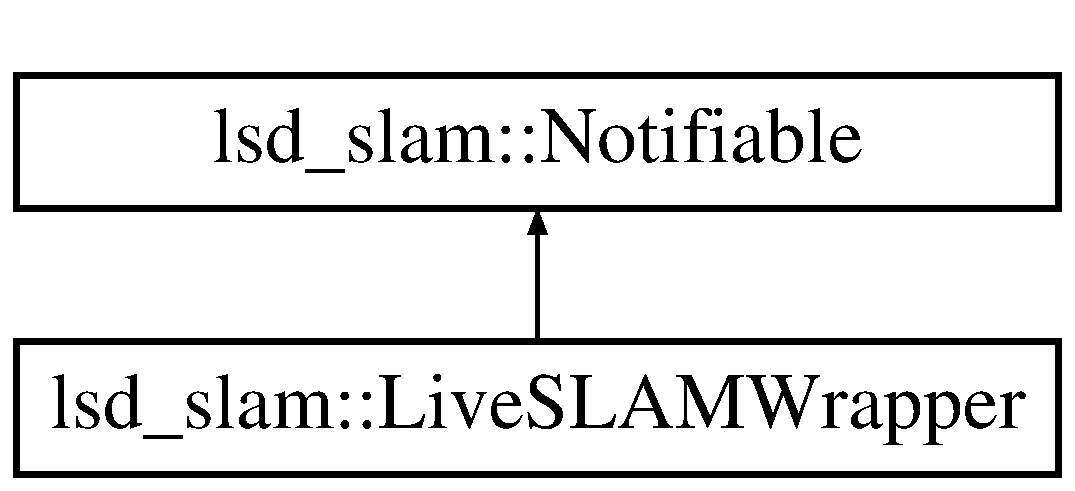
\includegraphics[height=2.000000cm]{structlsd__slam_1_1_live_s_l_a_m_wrapper}
\end{center}
\end{figure}
\subsection*{Public Member Functions}
\begin{DoxyCompactItemize}
\item 
\hypertarget{structlsd__slam_1_1_live_s_l_a_m_wrapper_a5eb56c2d74bb9b1f62e255f66361a1df}{E\-I\-G\-E\-N\-\_\-\-M\-A\-K\-E\-\_\-\-A\-L\-I\-G\-N\-E\-D\-\_\-\-O\-P\-E\-R\-A\-T\-O\-R\-\_\-\-N\-E\-W {\bfseries Live\-S\-L\-A\-M\-Wrapper} (\hyperlink{classlsd__slam_1_1_input_image_stream}{Input\-Image\-Stream} $\ast$image\-Stream, \hyperlink{classlsd__slam_1_1_output3_d_wrapper}{Output3\-D\-Wrapper} $\ast$output\-Wrapper)}\label{structlsd__slam_1_1_live_s_l_a_m_wrapper_a5eb56c2d74bb9b1f62e255f66361a1df}

\item 
\hyperlink{structlsd__slam_1_1_live_s_l_a_m_wrapper_a2e30a399280b41b721fe4a3a7cde580c}{$\sim$\-Live\-S\-L\-A\-M\-Wrapper} ()
\item 
void \hyperlink{structlsd__slam_1_1_live_s_l_a_m_wrapper_acca18b3dfae9dbfdb263fe5e40b03620}{Loop} ()
\item 
void \hyperlink{structlsd__slam_1_1_live_s_l_a_m_wrapper_af8c039c0c5a958f81aae837ceb01f1ff}{request\-Reset} ()
\item 
void \hyperlink{structlsd__slam_1_1_live_s_l_a_m_wrapper_aae9dfbb330f310d4f546456981459820}{reset\-All} ()
\item 
void \hyperlink{structlsd__slam_1_1_live_s_l_a_m_wrapper_a74585ef613514945d32c8594d3d24741}{new\-Image\-Callback} (const cv\-::\-Mat \&img, \hyperlink{classlsd__slam_1_1_timestamp}{Timestamp} img\-Time)
\item 
void \hyperlink{structlsd__slam_1_1_live_s_l_a_m_wrapper_a7324cecc197f65e911f6526fb3c3ac19}{log\-Camera\-Pose} (const S\-E3 \&cam\-To\-World, double time)
\item 
\hypertarget{structlsd__slam_1_1_live_s_l_a_m_wrapper_ac0f6675577df26d98c22e2549f3fcb19}{\hyperlink{classlsd__slam_1_1_slam_system}{Slam\-System} $\ast$ {\bfseries get\-Slam\-System} ()}\label{structlsd__slam_1_1_live_s_l_a_m_wrapper_ac0f6675577df26d98c22e2549f3fcb19}

\end{DoxyCompactItemize}
\subsection*{Friends}
\begin{DoxyCompactItemize}
\item 
\hypertarget{structlsd__slam_1_1_live_s_l_a_m_wrapper_ab3d0959819168d455e4122fa021df560}{class {\bfseries Live\-S\-L\-A\-M\-Wrapper\-R\-O\-S}}\label{structlsd__slam_1_1_live_s_l_a_m_wrapper_ab3d0959819168d455e4122fa021df560}

\end{DoxyCompactItemize}
\subsection*{Additional Inherited Members}


\subsection{Constructor \& Destructor Documentation}
\hypertarget{structlsd__slam_1_1_live_s_l_a_m_wrapper_a2e30a399280b41b721fe4a3a7cde580c}{\index{lsd\-\_\-slam\-::\-Live\-S\-L\-A\-M\-Wrapper@{lsd\-\_\-slam\-::\-Live\-S\-L\-A\-M\-Wrapper}!$\sim$\-Live\-S\-L\-A\-M\-Wrapper@{$\sim$\-Live\-S\-L\-A\-M\-Wrapper}}
\index{$\sim$\-Live\-S\-L\-A\-M\-Wrapper@{$\sim$\-Live\-S\-L\-A\-M\-Wrapper}!lsd_slam::LiveSLAMWrapper@{lsd\-\_\-slam\-::\-Live\-S\-L\-A\-M\-Wrapper}}
\subsubsection[{$\sim$\-Live\-S\-L\-A\-M\-Wrapper}]{\setlength{\rightskip}{0pt plus 5cm}lsd\-\_\-slam\-::\-Live\-S\-L\-A\-M\-Wrapper\-::$\sim$\-Live\-S\-L\-A\-M\-Wrapper (
\begin{DoxyParamCaption}
{}
\end{DoxyParamCaption}
)}}\label{structlsd__slam_1_1_live_s_l_a_m_wrapper_a2e30a399280b41b721fe4a3a7cde580c}
Destructor. 

\subsection{Member Function Documentation}
\hypertarget{structlsd__slam_1_1_live_s_l_a_m_wrapper_a7324cecc197f65e911f6526fb3c3ac19}{\index{lsd\-\_\-slam\-::\-Live\-S\-L\-A\-M\-Wrapper@{lsd\-\_\-slam\-::\-Live\-S\-L\-A\-M\-Wrapper}!log\-Camera\-Pose@{log\-Camera\-Pose}}
\index{log\-Camera\-Pose@{log\-Camera\-Pose}!lsd_slam::LiveSLAMWrapper@{lsd\-\_\-slam\-::\-Live\-S\-L\-A\-M\-Wrapper}}
\subsubsection[{log\-Camera\-Pose}]{\setlength{\rightskip}{0pt plus 5cm}void lsd\-\_\-slam\-::\-Live\-S\-L\-A\-M\-Wrapper\-::log\-Camera\-Pose (
\begin{DoxyParamCaption}
\item[{const S\-E3 \&}]{cam\-To\-World, }
\item[{double}]{time}
\end{DoxyParamCaption}
)}}\label{structlsd__slam_1_1_live_s_l_a_m_wrapper_a7324cecc197f65e911f6526fb3c3ac19}
Writes the given time and pose to the out\-File. \hypertarget{structlsd__slam_1_1_live_s_l_a_m_wrapper_acca18b3dfae9dbfdb263fe5e40b03620}{\index{lsd\-\_\-slam\-::\-Live\-S\-L\-A\-M\-Wrapper@{lsd\-\_\-slam\-::\-Live\-S\-L\-A\-M\-Wrapper}!Loop@{Loop}}
\index{Loop@{Loop}!lsd_slam::LiveSLAMWrapper@{lsd\-\_\-slam\-::\-Live\-S\-L\-A\-M\-Wrapper}}
\subsubsection[{Loop}]{\setlength{\rightskip}{0pt plus 5cm}void lsd\-\_\-slam\-::\-Live\-S\-L\-A\-M\-Wrapper\-::\-Loop (
\begin{DoxyParamCaption}
{}
\end{DoxyParamCaption}
)}}\label{structlsd__slam_1_1_live_s_l_a_m_wrapper_acca18b3dfae9dbfdb263fe5e40b03620}
Runs the main processing loop. Will never return. \hypertarget{structlsd__slam_1_1_live_s_l_a_m_wrapper_a74585ef613514945d32c8594d3d24741}{\index{lsd\-\_\-slam\-::\-Live\-S\-L\-A\-M\-Wrapper@{lsd\-\_\-slam\-::\-Live\-S\-L\-A\-M\-Wrapper}!new\-Image\-Callback@{new\-Image\-Callback}}
\index{new\-Image\-Callback@{new\-Image\-Callback}!lsd_slam::LiveSLAMWrapper@{lsd\-\_\-slam\-::\-Live\-S\-L\-A\-M\-Wrapper}}
\subsubsection[{new\-Image\-Callback}]{\setlength{\rightskip}{0pt plus 5cm}void lsd\-\_\-slam\-::\-Live\-S\-L\-A\-M\-Wrapper\-::new\-Image\-Callback (
\begin{DoxyParamCaption}
\item[{const cv\-::\-Mat \&}]{img, }
\item[{{\bf Timestamp}}]{img\-Time}
\end{DoxyParamCaption}
)}}\label{structlsd__slam_1_1_live_s_l_a_m_wrapper_a74585ef613514945d32c8594d3d24741}
Callback function for new R\-G\-B images. \hypertarget{structlsd__slam_1_1_live_s_l_a_m_wrapper_af8c039c0c5a958f81aae837ceb01f1ff}{\index{lsd\-\_\-slam\-::\-Live\-S\-L\-A\-M\-Wrapper@{lsd\-\_\-slam\-::\-Live\-S\-L\-A\-M\-Wrapper}!request\-Reset@{request\-Reset}}
\index{request\-Reset@{request\-Reset}!lsd_slam::LiveSLAMWrapper@{lsd\-\_\-slam\-::\-Live\-S\-L\-A\-M\-Wrapper}}
\subsubsection[{request\-Reset}]{\setlength{\rightskip}{0pt plus 5cm}void lsd\-\_\-slam\-::\-Live\-S\-L\-A\-M\-Wrapper\-::request\-Reset (
\begin{DoxyParamCaption}
{}
\end{DoxyParamCaption}
)}}\label{structlsd__slam_1_1_live_s_l_a_m_wrapper_af8c039c0c5a958f81aae837ceb01f1ff}
Requests a reset from a different thread. \hypertarget{structlsd__slam_1_1_live_s_l_a_m_wrapper_aae9dfbb330f310d4f546456981459820}{\index{lsd\-\_\-slam\-::\-Live\-S\-L\-A\-M\-Wrapper@{lsd\-\_\-slam\-::\-Live\-S\-L\-A\-M\-Wrapper}!reset\-All@{reset\-All}}
\index{reset\-All@{reset\-All}!lsd_slam::LiveSLAMWrapper@{lsd\-\_\-slam\-::\-Live\-S\-L\-A\-M\-Wrapper}}
\subsubsection[{reset\-All}]{\setlength{\rightskip}{0pt plus 5cm}void lsd\-\_\-slam\-::\-Live\-S\-L\-A\-M\-Wrapper\-::reset\-All (
\begin{DoxyParamCaption}
{}
\end{DoxyParamCaption}
)}}\label{structlsd__slam_1_1_live_s_l_a_m_wrapper_aae9dfbb330f310d4f546456981459820}
Resets everything, starting the odometry from the beginning again. 

The documentation for this struct was generated from the following files\-:\begin{DoxyCompactItemize}
\item 
/home/king/rgbd-\/slam-\/lets-\/do-\/it/9-\/doxygen/lsd\-\_\-slam/lsd\-\_\-slam\-\_\-core/src/Live\-S\-L\-A\-M\-Wrapper.\-h\item 
/home/king/rgbd-\/slam-\/lets-\/do-\/it/9-\/doxygen/lsd\-\_\-slam/lsd\-\_\-slam\-\_\-core/src/Live\-S\-L\-A\-M\-Wrapper.\-cpp\end{DoxyCompactItemize}

\hypertarget{classlsd__slam_1_1_notifiable}{\section{lsd\-\_\-slam\-:\-:Notifiable Class Reference}
\label{classlsd__slam_1_1_notifiable}\index{lsd\-\_\-slam\-::\-Notifiable@{lsd\-\_\-slam\-::\-Notifiable}}
}


{\ttfamily \#include $<$Notify\-Buffer.\-h$>$}

Inheritance diagram for lsd\-\_\-slam\-:\-:Notifiable\-:\begin{figure}[H]
\begin{center}
\leavevmode
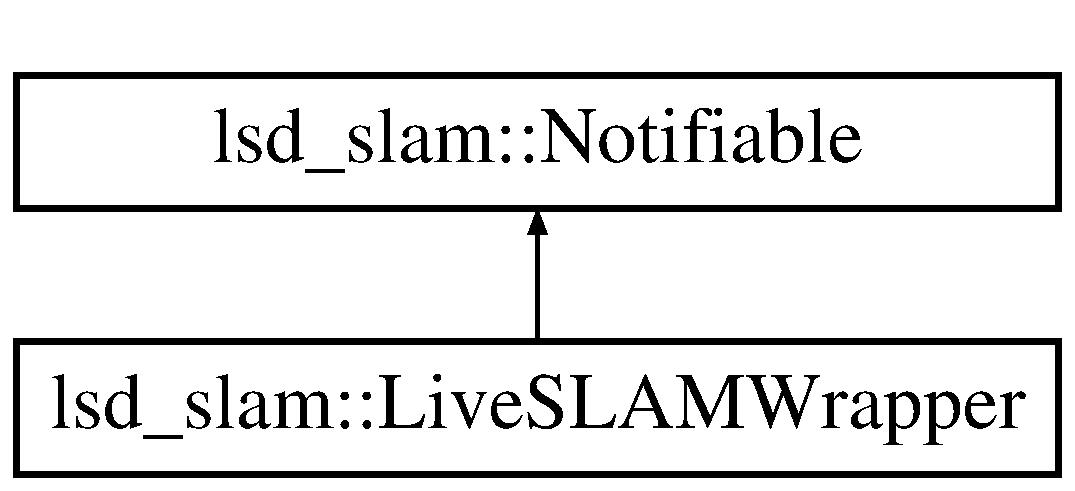
\includegraphics[height=2.000000cm]{classlsd__slam_1_1_notifiable}
\end{center}
\end{figure}
\subsection*{Public Member Functions}
\begin{DoxyCompactItemize}
\item 
void \hyperlink{classlsd__slam_1_1_notifiable_a57feb058f865c0e693ca3806416d84ac}{notify} ()
\end{DoxyCompactItemize}
\subsection*{Protected Attributes}
\begin{DoxyCompactItemize}
\item 
\hypertarget{classlsd__slam_1_1_notifiable_a0b321c3c5b0db6ab8bb689c821384246}{boost\-::condition {\bfseries notify\-Condition}}\label{classlsd__slam_1_1_notifiable_a0b321c3c5b0db6ab8bb689c821384246}

\end{DoxyCompactItemize}


\subsection{Detailed Description}
Contains an internal boost\-::condition on which notify\-\_\-all() can be called from the outside. 

\subsection{Member Function Documentation}
\hypertarget{classlsd__slam_1_1_notifiable_a57feb058f865c0e693ca3806416d84ac}{\index{lsd\-\_\-slam\-::\-Notifiable@{lsd\-\_\-slam\-::\-Notifiable}!notify@{notify}}
\index{notify@{notify}!lsd_slam::Notifiable@{lsd\-\_\-slam\-::\-Notifiable}}
\subsubsection[{notify}]{\setlength{\rightskip}{0pt plus 5cm}void lsd\-\_\-slam\-::\-Notifiable\-::notify (
\begin{DoxyParamCaption}
{}
\end{DoxyParamCaption}
)\hspace{0.3cm}{\ttfamily [inline]}}}\label{classlsd__slam_1_1_notifiable_a57feb058f865c0e693ca3806416d84ac}
Calls notify\-\_\-all() on notify\-Condition. 

The documentation for this class was generated from the following file\-:\begin{DoxyCompactItemize}
\item 
/home/king/rgbd-\/slam-\/lets-\/do-\/it/9-\/doxygen/lsd\-\_\-slam/lsd\-\_\-slam\-\_\-core/src/\-I\-O\-Wrapper/Notify\-Buffer.\-h\end{DoxyCompactItemize}

\hypertarget{classlsd__slam_1_1_notify_buffer}{\section{lsd\-\_\-slam\-:\-:Notify\-Buffer$<$ T $>$ Class Template Reference}
\label{classlsd__slam_1_1_notify_buffer}\index{lsd\-\_\-slam\-::\-Notify\-Buffer$<$ T $>$@{lsd\-\_\-slam\-::\-Notify\-Buffer$<$ T $>$}}
}


{\ttfamily \#include $<$Notify\-Buffer.\-h$>$}

\subsection*{Public Member Functions}
\begin{DoxyCompactItemize}
\item 
\hyperlink{classlsd__slam_1_1_notify_buffer_a38032ad4284b2e1f5e92812c52f162d6}{Notify\-Buffer} (int buffer\-Size)
\item 
\hyperlink{classlsd__slam_1_1_notify_buffer_a3933bbbf4b48593399950b251e677299}{Notify\-Buffer} (int buffer\-Size, \hyperlink{classlsd__slam_1_1_notifiable}{Notifiable} $\ast$receiver)
\item 
void \hyperlink{classlsd__slam_1_1_notify_buffer_abff5c7a6af7790acfc5cc2f83ae541c0}{set\-Receiver} (\hyperlink{classlsd__slam_1_1_notifiable}{Notifiable} $\ast$receiver)
\item 
bool \hyperlink{classlsd__slam_1_1_notify_buffer_a04532ca3a71447a2b8fa51f5e9db8dd8}{push\-Back} (const T \&object)
\item 
int \hyperlink{classlsd__slam_1_1_notify_buffer_ac077a4a4bb56f5dd9acd551c7c56a3a3}{size} ()
\item 
T \hyperlink{classlsd__slam_1_1_notify_buffer_a25b914af4aa669d39f8123364cfbb541}{first} ()
\item 
T \hyperlink{classlsd__slam_1_1_notify_buffer_ac16d9abdd418c98b87a8117a9b97eaf6}{pop\-Front} ()
\item 
boost\-::recursive\-\_\-mutex \& \hyperlink{classlsd__slam_1_1_notify_buffer_abd90fea9478812fb5b2a0333a2480f23}{get\-Mutex} ()
\end{DoxyCompactItemize}


\subsection{Detailed Description}
\subsubsection*{template$<$typename T$>$class lsd\-\_\-slam\-::\-Notify\-Buffer$<$ T $>$}

Thread-\/safe limited-\/size buffer which may notify a specific object when a new item becomes available. 

\subsection{Constructor \& Destructor Documentation}
\hypertarget{classlsd__slam_1_1_notify_buffer_a38032ad4284b2e1f5e92812c52f162d6}{\index{lsd\-\_\-slam\-::\-Notify\-Buffer@{lsd\-\_\-slam\-::\-Notify\-Buffer}!Notify\-Buffer@{Notify\-Buffer}}
\index{Notify\-Buffer@{Notify\-Buffer}!lsd_slam::NotifyBuffer@{lsd\-\_\-slam\-::\-Notify\-Buffer}}
\subsubsection[{Notify\-Buffer}]{\setlength{\rightskip}{0pt plus 5cm}template$<$typename T$>$ {\bf lsd\-\_\-slam\-::\-Notify\-Buffer}$<$ T $>$\-::{\bf Notify\-Buffer} (
\begin{DoxyParamCaption}
\item[{int}]{buffer\-Size}
\end{DoxyParamCaption}
)\hspace{0.3cm}{\ttfamily [inline]}}}\label{classlsd__slam_1_1_notify_buffer_a38032ad4284b2e1f5e92812c52f162d6}
Creates a queue with the given maximum size. \hypertarget{classlsd__slam_1_1_notify_buffer_a3933bbbf4b48593399950b251e677299}{\index{lsd\-\_\-slam\-::\-Notify\-Buffer@{lsd\-\_\-slam\-::\-Notify\-Buffer}!Notify\-Buffer@{Notify\-Buffer}}
\index{Notify\-Buffer@{Notify\-Buffer}!lsd_slam::NotifyBuffer@{lsd\-\_\-slam\-::\-Notify\-Buffer}}
\subsubsection[{Notify\-Buffer}]{\setlength{\rightskip}{0pt plus 5cm}template$<$typename T$>$ {\bf lsd\-\_\-slam\-::\-Notify\-Buffer}$<$ T $>$\-::{\bf Notify\-Buffer} (
\begin{DoxyParamCaption}
\item[{int}]{buffer\-Size, }
\item[{{\bf Notifiable} $\ast$}]{receiver}
\end{DoxyParamCaption}
)\hspace{0.3cm}{\ttfamily [inline]}}}\label{classlsd__slam_1_1_notify_buffer_a3933bbbf4b48593399950b251e677299}
Creates a queue with the given maximum size and \hyperlink{classlsd__slam_1_1_notifiable}{Notifiable} instance which will be notified when a new object becomes available. 

\subsection{Member Function Documentation}
\hypertarget{classlsd__slam_1_1_notify_buffer_a25b914af4aa669d39f8123364cfbb541}{\index{lsd\-\_\-slam\-::\-Notify\-Buffer@{lsd\-\_\-slam\-::\-Notify\-Buffer}!first@{first}}
\index{first@{first}!lsd_slam::NotifyBuffer@{lsd\-\_\-slam\-::\-Notify\-Buffer}}
\subsubsection[{first}]{\setlength{\rightskip}{0pt plus 5cm}template$<$typename T$>$ T {\bf lsd\-\_\-slam\-::\-Notify\-Buffer}$<$ T $>$\-::first (
\begin{DoxyParamCaption}
{}
\end{DoxyParamCaption}
)\hspace{0.3cm}{\ttfamily [inline]}}}\label{classlsd__slam_1_1_notify_buffer_a25b914af4aa669d39f8123364cfbb541}
Returns a copy of the first object. \hypertarget{classlsd__slam_1_1_notify_buffer_abd90fea9478812fb5b2a0333a2480f23}{\index{lsd\-\_\-slam\-::\-Notify\-Buffer@{lsd\-\_\-slam\-::\-Notify\-Buffer}!get\-Mutex@{get\-Mutex}}
\index{get\-Mutex@{get\-Mutex}!lsd_slam::NotifyBuffer@{lsd\-\_\-slam\-::\-Notify\-Buffer}}
\subsubsection[{get\-Mutex}]{\setlength{\rightskip}{0pt plus 5cm}template$<$typename T$>$ boost\-::recursive\-\_\-mutex\& {\bf lsd\-\_\-slam\-::\-Notify\-Buffer}$<$ T $>$\-::get\-Mutex (
\begin{DoxyParamCaption}
{}
\end{DoxyParamCaption}
)\hspace{0.3cm}{\ttfamily [inline]}}}\label{classlsd__slam_1_1_notify_buffer_abd90fea9478812fb5b2a0333a2480f23}
Returns the buffer access mutex. Must be locked when checking \hyperlink{classlsd__slam_1_1_notify_buffer_ac077a4a4bb56f5dd9acd551c7c56a3a3}{size()} and waiting if \hyperlink{classlsd__slam_1_1_notify_buffer_ac077a4a4bb56f5dd9acd551c7c56a3a3}{size()} == 0. \hypertarget{classlsd__slam_1_1_notify_buffer_ac16d9abdd418c98b87a8117a9b97eaf6}{\index{lsd\-\_\-slam\-::\-Notify\-Buffer@{lsd\-\_\-slam\-::\-Notify\-Buffer}!pop\-Front@{pop\-Front}}
\index{pop\-Front@{pop\-Front}!lsd_slam::NotifyBuffer@{lsd\-\_\-slam\-::\-Notify\-Buffer}}
\subsubsection[{pop\-Front}]{\setlength{\rightskip}{0pt plus 5cm}template$<$typename T$>$ T {\bf lsd\-\_\-slam\-::\-Notify\-Buffer}$<$ T $>$\-::pop\-Front (
\begin{DoxyParamCaption}
{}
\end{DoxyParamCaption}
)\hspace{0.3cm}{\ttfamily [inline]}}}\label{classlsd__slam_1_1_notify_buffer_ac16d9abdd418c98b87a8117a9b97eaf6}
Removes the first object and returns a copy of it.

If there is no object in the queue, blocks until one is available. \hypertarget{classlsd__slam_1_1_notify_buffer_a04532ca3a71447a2b8fa51f5e9db8dd8}{\index{lsd\-\_\-slam\-::\-Notify\-Buffer@{lsd\-\_\-slam\-::\-Notify\-Buffer}!push\-Back@{push\-Back}}
\index{push\-Back@{push\-Back}!lsd_slam::NotifyBuffer@{lsd\-\_\-slam\-::\-Notify\-Buffer}}
\subsubsection[{push\-Back}]{\setlength{\rightskip}{0pt plus 5cm}template$<$typename T$>$ bool {\bf lsd\-\_\-slam\-::\-Notify\-Buffer}$<$ T $>$\-::push\-Back (
\begin{DoxyParamCaption}
\item[{const T \&}]{object}
\end{DoxyParamCaption}
)\hspace{0.3cm}{\ttfamily [inline]}}}\label{classlsd__slam_1_1_notify_buffer_a04532ca3a71447a2b8fa51f5e9db8dd8}
Adds an object to the back of the queue.

If the queue is full already, discards the object. Returns if there was enough space to add the object. \hypertarget{classlsd__slam_1_1_notify_buffer_abff5c7a6af7790acfc5cc2f83ae541c0}{\index{lsd\-\_\-slam\-::\-Notify\-Buffer@{lsd\-\_\-slam\-::\-Notify\-Buffer}!set\-Receiver@{set\-Receiver}}
\index{set\-Receiver@{set\-Receiver}!lsd_slam::NotifyBuffer@{lsd\-\_\-slam\-::\-Notify\-Buffer}}
\subsubsection[{set\-Receiver}]{\setlength{\rightskip}{0pt plus 5cm}template$<$typename T$>$ void {\bf lsd\-\_\-slam\-::\-Notify\-Buffer}$<$ T $>$\-::set\-Receiver (
\begin{DoxyParamCaption}
\item[{{\bf Notifiable} $\ast$}]{receiver}
\end{DoxyParamCaption}
)\hspace{0.3cm}{\ttfamily [inline]}}}\label{classlsd__slam_1_1_notify_buffer_abff5c7a6af7790acfc5cc2f83ae541c0}
Sets the notification receiver.

The receiver can be nullptr to disable notifications. \hypertarget{classlsd__slam_1_1_notify_buffer_ac077a4a4bb56f5dd9acd551c7c56a3a3}{\index{lsd\-\_\-slam\-::\-Notify\-Buffer@{lsd\-\_\-slam\-::\-Notify\-Buffer}!size@{size}}
\index{size@{size}!lsd_slam::NotifyBuffer@{lsd\-\_\-slam\-::\-Notify\-Buffer}}
\subsubsection[{size}]{\setlength{\rightskip}{0pt plus 5cm}template$<$typename T$>$ int {\bf lsd\-\_\-slam\-::\-Notify\-Buffer}$<$ T $>$\-::size (
\begin{DoxyParamCaption}
{}
\end{DoxyParamCaption}
)\hspace{0.3cm}{\ttfamily [inline]}}}\label{classlsd__slam_1_1_notify_buffer_ac077a4a4bb56f5dd9acd551c7c56a3a3}
Returns the number of objects in the buffer. 

The documentation for this class was generated from the following file\-:\begin{DoxyCompactItemize}
\item 
/home/king/rgbd-\/slam-\/lets-\/do-\/it/9-\/doxygen/lsd\-\_\-slam/lsd\-\_\-slam\-\_\-core/src/\-I\-O\-Wrapper/Notify\-Buffer.\-h\end{DoxyCompactItemize}

\hypertarget{classlsd__slam_1_1_output3_d_wrapper}{\section{lsd\-\_\-slam\-:\-:Output3\-D\-Wrapper Class Reference}
\label{classlsd__slam_1_1_output3_d_wrapper}\index{lsd\-\_\-slam\-::\-Output3\-D\-Wrapper@{lsd\-\_\-slam\-::\-Output3\-D\-Wrapper}}
}


{\ttfamily \#include $<$Output3\-D\-Wrapper.\-h$>$}

Inheritance diagram for lsd\-\_\-slam\-:\-:Output3\-D\-Wrapper\-:\begin{figure}[H]
\begin{center}
\leavevmode
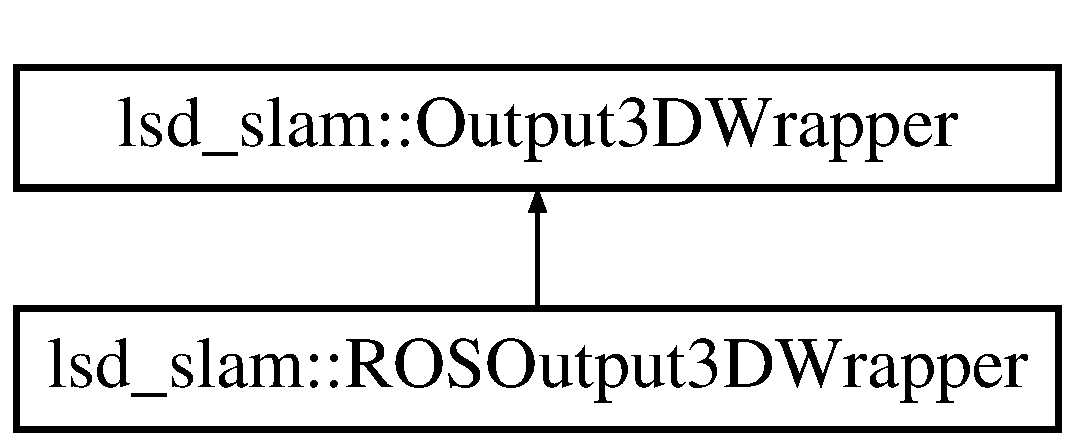
\includegraphics[height=2.000000cm]{classlsd__slam_1_1_output3_d_wrapper}
\end{center}
\end{figure}
\subsection*{Public Member Functions}
\begin{DoxyCompactItemize}
\item 
\hypertarget{classlsd__slam_1_1_output3_d_wrapper_a4b91b74ec0c7c8b4fc7d80beb4853c35}{virtual void {\bfseries publish\-Keyframe\-Graph} (\hyperlink{classlsd__slam_1_1_key_frame_graph}{Key\-Frame\-Graph} $\ast$graph)}\label{classlsd__slam_1_1_output3_d_wrapper_a4b91b74ec0c7c8b4fc7d80beb4853c35}

\item 
\hypertarget{classlsd__slam_1_1_output3_d_wrapper_a524f65c21ef553f626a75e24e3ea10f5}{virtual void {\bfseries publish\-Keyframe} (\hyperlink{classlsd__slam_1_1_frame}{Frame} $\ast$kf)}\label{classlsd__slam_1_1_output3_d_wrapper_a524f65c21ef553f626a75e24e3ea10f5}

\item 
\hypertarget{classlsd__slam_1_1_output3_d_wrapper_a679c2193d1eba147a88d362eda088d72}{virtual void {\bfseries publish\-Tracked\-Frame} (\hyperlink{classlsd__slam_1_1_frame}{Frame} $\ast$kf)}\label{classlsd__slam_1_1_output3_d_wrapper_a679c2193d1eba147a88d362eda088d72}

\item 
\hypertarget{classlsd__slam_1_1_output3_d_wrapper_aff80413d7e0f925b673da9368be657d0}{virtual void {\bfseries publish\-Trajectory} (std\-::vector$<$ Eigen\-::\-Matrix$<$ float, 3, 1 $>$$>$ trajectory, std\-::string identifier)}\label{classlsd__slam_1_1_output3_d_wrapper_aff80413d7e0f925b673da9368be657d0}

\item 
\hypertarget{classlsd__slam_1_1_output3_d_wrapper_a72ad5d3823f98413b0b565d6315f781c}{virtual void {\bfseries publish\-Trajectory\-Increment} (Eigen\-::\-Matrix$<$ float, 3, 1 $>$ pt, std\-::string identifier)}\label{classlsd__slam_1_1_output3_d_wrapper_a72ad5d3823f98413b0b565d6315f781c}

\item 
\hypertarget{classlsd__slam_1_1_output3_d_wrapper_a0b3bd60770aa486fc36465a5275ab1cd}{virtual void {\bfseries publish\-Debug\-Info} (Eigen\-::\-Matrix$<$ float, 20, 1 $>$ data)}\label{classlsd__slam_1_1_output3_d_wrapper_a0b3bd60770aa486fc36465a5275ab1cd}

\end{DoxyCompactItemize}


\subsection{Detailed Description}
Virtual 3\-D display object. 

The documentation for this class was generated from the following file\-:\begin{DoxyCompactItemize}
\item 
/home/king/rgbd-\/slam-\/lets-\/do-\/it/9-\/doxygen/lsd\-\_\-slam/lsd\-\_\-slam\-\_\-core/src/\-I\-O\-Wrapper/Output3\-D\-Wrapper.\-h\end{DoxyCompactItemize}

\hypertarget{classlsd__slam_1_1_relocalizer}{\section{lsd\-\_\-slam\-:\-:Relocalizer Class Reference}
\label{classlsd__slam_1_1_relocalizer}\index{lsd\-\_\-slam\-::\-Relocalizer@{lsd\-\_\-slam\-::\-Relocalizer}}
}
\subsection*{Public Member Functions}
\begin{DoxyCompactItemize}
\item 
\hypertarget{classlsd__slam_1_1_relocalizer_acd060c9dc0f2c1ae667f517a1f3e7947}{{\bfseries Relocalizer} (int w, int h, Eigen\-::\-Matrix3f K)}\label{classlsd__slam_1_1_relocalizer_acd060c9dc0f2c1ae667f517a1f3e7947}

\item 
\hypertarget{classlsd__slam_1_1_relocalizer_a55f025b2393347238dd7e039c04cd55f}{void {\bfseries update\-Current\-Frame} (std\-::shared\-\_\-ptr$<$ \hyperlink{classlsd__slam_1_1_frame}{Frame} $>$ current\-Frame)}\label{classlsd__slam_1_1_relocalizer_a55f025b2393347238dd7e039c04cd55f}

\item 
\hypertarget{classlsd__slam_1_1_relocalizer_ae4dd8af1a09287333b2f7a22ac5ef99d}{void {\bfseries start} (std\-::vector$<$ \hyperlink{classlsd__slam_1_1_frame}{Frame} $\ast$, Eigen\-::aligned\-\_\-allocator$<$ \hyperlink{classlsd__slam_1_1_frame}{lsd\-\_\-slam\-::\-Frame} $\ast$ $>$ $>$ \&all\-Keyframes\-List)}\label{classlsd__slam_1_1_relocalizer_ae4dd8af1a09287333b2f7a22ac5ef99d}

\item 
\hypertarget{classlsd__slam_1_1_relocalizer_a74488e97a8183f671a5e0b34d81e9b88}{void {\bfseries stop} ()}\label{classlsd__slam_1_1_relocalizer_a74488e97a8183f671a5e0b34d81e9b88}

\item 
\hypertarget{classlsd__slam_1_1_relocalizer_a3c06e60e0788f2203160d46825745492}{bool {\bfseries wait\-Result} (int milliseconds)}\label{classlsd__slam_1_1_relocalizer_a3c06e60e0788f2203160d46825745492}

\item 
\hypertarget{classlsd__slam_1_1_relocalizer_a2c50009413c4f6d2d8de3f9e8c9c7272}{void {\bfseries get\-Result} (\hyperlink{classlsd__slam_1_1_frame}{Frame} $\ast$\&out\-\_\-keyframe, std\-::shared\-\_\-ptr$<$ \hyperlink{classlsd__slam_1_1_frame}{Frame} $>$ \&frame, int \&out\-\_\-successful\-Frame\-I\-D, S\-E3 \&out\-\_\-frame\-To\-Keyframe)}\label{classlsd__slam_1_1_relocalizer_a2c50009413c4f6d2d8de3f9e8c9c7272}

\end{DoxyCompactItemize}
\subsection*{Public Attributes}
\begin{DoxyCompactItemize}
\item 
\hypertarget{classlsd__slam_1_1_relocalizer_a771108ba996cd0bc8392e256b4060db3}{bool {\bfseries is\-Running}}\label{classlsd__slam_1_1_relocalizer_a771108ba996cd0bc8392e256b4060db3}

\end{DoxyCompactItemize}


The documentation for this class was generated from the following files\-:\begin{DoxyCompactItemize}
\item 
/home/king/rgbd-\/slam-\/lets-\/do-\/it/9-\/doxygen/lsd\-\_\-slam/lsd\-\_\-slam\-\_\-core/src/\-Tracking/Relocalizer.\-h\item 
/home/king/rgbd-\/slam-\/lets-\/do-\/it/9-\/doxygen/lsd\-\_\-slam/lsd\-\_\-slam\-\_\-core/src/\-Tracking/Relocalizer.\-cpp\end{DoxyCompactItemize}

\hypertarget{classlsd__slam_1_1_r_o_s_image_stream_thread}{\section{lsd\-\_\-slam\-:\-:R\-O\-S\-Image\-Stream\-Thread Class Reference}
\label{classlsd__slam_1_1_r_o_s_image_stream_thread}\index{lsd\-\_\-slam\-::\-R\-O\-S\-Image\-Stream\-Thread@{lsd\-\_\-slam\-::\-R\-O\-S\-Image\-Stream\-Thread}}
}


{\ttfamily \#include $<$R\-O\-S\-Image\-Stream\-Thread.\-h$>$}

Inheritance diagram for lsd\-\_\-slam\-:\-:R\-O\-S\-Image\-Stream\-Thread\-:\begin{figure}[H]
\begin{center}
\leavevmode
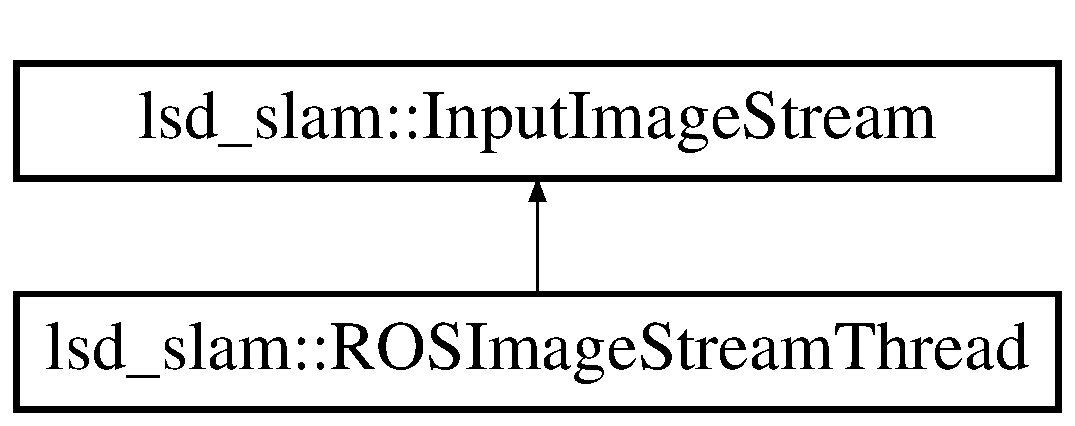
\includegraphics[height=2.000000cm]{classlsd__slam_1_1_r_o_s_image_stream_thread}
\end{center}
\end{figure}
\subsection*{Public Member Functions}
\begin{DoxyCompactItemize}
\item 
void \hyperlink{classlsd__slam_1_1_r_o_s_image_stream_thread_a8d20574101837956cdebe14761c368fc}{run} ()
\item 
\hypertarget{classlsd__slam_1_1_r_o_s_image_stream_thread_a5567cf59a4603c5bfe818ef78c58b1c0}{void {\bfseries set\-Calibration} (std\-::string file)}\label{classlsd__slam_1_1_r_o_s_image_stream_thread_a5567cf59a4603c5bfe818ef78c58b1c0}

\item 
void \hyperlink{classlsd__slam_1_1_r_o_s_image_stream_thread_a93b7630a508fd900b8bfaec19235016f}{operator()} ()
\item 
\hypertarget{classlsd__slam_1_1_r_o_s_image_stream_thread_a2d10e72133d60039a752cbbe8a7140e8}{void {\bfseries vid\-Cb} (const sensor\-\_\-msgs\-::\-Image\-Const\-Ptr img)}\label{classlsd__slam_1_1_r_o_s_image_stream_thread_a2d10e72133d60039a752cbbe8a7140e8}

\item 
\hypertarget{classlsd__slam_1_1_r_o_s_image_stream_thread_abfe05966e4a0e232e5433fc27bd78139}{void {\bfseries info\-Cb} (const sensor\-\_\-msgs\-::\-Camera\-Info\-Const\-Ptr info)}\label{classlsd__slam_1_1_r_o_s_image_stream_thread_abfe05966e4a0e232e5433fc27bd78139}

\end{DoxyCompactItemize}
\subsection*{Additional Inherited Members}


\subsection{Detailed Description}
Image stream provider using R\-O\-S messages. 

\subsection{Member Function Documentation}
\hypertarget{classlsd__slam_1_1_r_o_s_image_stream_thread_a93b7630a508fd900b8bfaec19235016f}{\index{lsd\-\_\-slam\-::\-R\-O\-S\-Image\-Stream\-Thread@{lsd\-\_\-slam\-::\-R\-O\-S\-Image\-Stream\-Thread}!operator()@{operator()}}
\index{operator()@{operator()}!lsd_slam::ROSImageStreamThread@{lsd\-\_\-slam\-::\-R\-O\-S\-Image\-Stream\-Thread}}
\subsubsection[{operator()}]{\setlength{\rightskip}{0pt plus 5cm}void lsd\-\_\-slam\-::\-R\-O\-S\-Image\-Stream\-Thread\-::operator() (
\begin{DoxyParamCaption}
{}
\end{DoxyParamCaption}
)}}\label{classlsd__slam_1_1_r_o_s_image_stream_thread_a93b7630a508fd900b8bfaec19235016f}
Thread main function. \hypertarget{classlsd__slam_1_1_r_o_s_image_stream_thread_a8d20574101837956cdebe14761c368fc}{\index{lsd\-\_\-slam\-::\-R\-O\-S\-Image\-Stream\-Thread@{lsd\-\_\-slam\-::\-R\-O\-S\-Image\-Stream\-Thread}!run@{run}}
\index{run@{run}!lsd_slam::ROSImageStreamThread@{lsd\-\_\-slam\-::\-R\-O\-S\-Image\-Stream\-Thread}}
\subsubsection[{run}]{\setlength{\rightskip}{0pt plus 5cm}void lsd\-\_\-slam\-::\-R\-O\-S\-Image\-Stream\-Thread\-::run (
\begin{DoxyParamCaption}
{}
\end{DoxyParamCaption}
)\hspace{0.3cm}{\ttfamily [virtual]}}}\label{classlsd__slam_1_1_r_o_s_image_stream_thread_a8d20574101837956cdebe14761c368fc}
Starts the thread. 

Reimplemented from \hyperlink{classlsd__slam_1_1_input_image_stream_a54d88ab343986e2a8f17d1ff5f5901be}{lsd\-\_\-slam\-::\-Input\-Image\-Stream}.



The documentation for this class was generated from the following files\-:\begin{DoxyCompactItemize}
\item 
/home/king/rgbd-\/slam-\/lets-\/do-\/it/9-\/doxygen/lsd\-\_\-slam/lsd\-\_\-slam\-\_\-core/src/\-I\-O\-Wrapper/\-R\-O\-S/R\-O\-S\-Image\-Stream\-Thread.\-h\item 
/home/king/rgbd-\/slam-\/lets-\/do-\/it/9-\/doxygen/lsd\-\_\-slam/lsd\-\_\-slam\-\_\-core/src/\-I\-O\-Wrapper/\-R\-O\-S/R\-O\-S\-Image\-Stream\-Thread.\-cpp\end{DoxyCompactItemize}

\hypertarget{classlsd__slam_1_1_r_o_s_output3_d_wrapper}{\section{lsd\-\_\-slam\-:\-:R\-O\-S\-Output3\-D\-Wrapper Class Reference}
\label{classlsd__slam_1_1_r_o_s_output3_d_wrapper}\index{lsd\-\_\-slam\-::\-R\-O\-S\-Output3\-D\-Wrapper@{lsd\-\_\-slam\-::\-R\-O\-S\-Output3\-D\-Wrapper}}
}


{\ttfamily \#include $<$R\-O\-S\-Output3\-D\-Wrapper.\-h$>$}

Inheritance diagram for lsd\-\_\-slam\-:\-:R\-O\-S\-Output3\-D\-Wrapper\-:\begin{figure}[H]
\begin{center}
\leavevmode
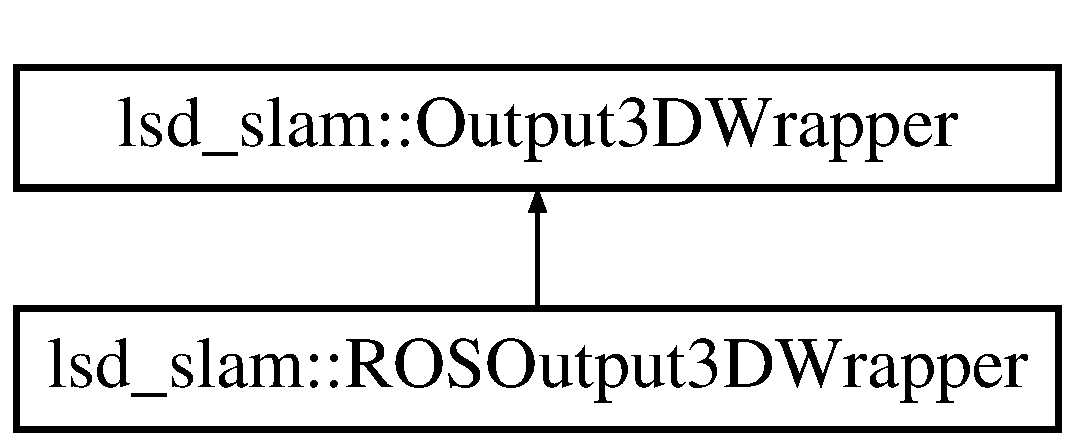
\includegraphics[height=2.000000cm]{classlsd__slam_1_1_r_o_s_output3_d_wrapper}
\end{center}
\end{figure}
\subsection*{Public Member Functions}
\begin{DoxyCompactItemize}
\item 
\hypertarget{classlsd__slam_1_1_r_o_s_output3_d_wrapper_a1b499d3c51fd2e9fb83880d7b1f7afd4}{{\bfseries R\-O\-S\-Output3\-D\-Wrapper} (int width, int height)}\label{classlsd__slam_1_1_r_o_s_output3_d_wrapper_a1b499d3c51fd2e9fb83880d7b1f7afd4}

\item 
\hypertarget{classlsd__slam_1_1_r_o_s_output3_d_wrapper_ae67d180442d8a24b8f3394ca236f3b72}{virtual void {\bfseries publish\-Keyframe\-Graph} (\hyperlink{classlsd__slam_1_1_key_frame_graph}{Key\-Frame\-Graph} $\ast$graph)}\label{classlsd__slam_1_1_r_o_s_output3_d_wrapper_ae67d180442d8a24b8f3394ca236f3b72}

\item 
\hypertarget{classlsd__slam_1_1_r_o_s_output3_d_wrapper_a19b724e2f3561a3bcd37809da33711a3}{virtual void {\bfseries publish\-Keyframe} (\hyperlink{classlsd__slam_1_1_frame}{Frame} $\ast$f)}\label{classlsd__slam_1_1_r_o_s_output3_d_wrapper_a19b724e2f3561a3bcd37809da33711a3}

\item 
\hypertarget{classlsd__slam_1_1_r_o_s_output3_d_wrapper_aa5144ddbec893f84408c74f01e7d9eff}{virtual void {\bfseries publish\-Tracked\-Frame} (\hyperlink{classlsd__slam_1_1_frame}{Frame} $\ast$f)}\label{classlsd__slam_1_1_r_o_s_output3_d_wrapper_aa5144ddbec893f84408c74f01e7d9eff}

\item 
\hypertarget{classlsd__slam_1_1_r_o_s_output3_d_wrapper_a015b676f34b19c67317470c2b976f4e9}{virtual void {\bfseries publish\-Trajectory} (std\-::vector$<$ Eigen\-::\-Matrix$<$ float, 3, 1 $>$$>$ trajectory, std\-::string identifier)}\label{classlsd__slam_1_1_r_o_s_output3_d_wrapper_a015b676f34b19c67317470c2b976f4e9}

\item 
\hypertarget{classlsd__slam_1_1_r_o_s_output3_d_wrapper_ad272713c3de1bf15fbbb7c453984d548}{virtual void {\bfseries publish\-Trajectory\-Increment} (Eigen\-::\-Matrix$<$ float, 3, 1 $>$ pt, std\-::string identifier)}\label{classlsd__slam_1_1_r_o_s_output3_d_wrapper_ad272713c3de1bf15fbbb7c453984d548}

\item 
\hypertarget{classlsd__slam_1_1_r_o_s_output3_d_wrapper_a9da72eca1e8b623c65bd647d0f7c3a73}{virtual void {\bfseries publish\-Debug\-Info} (Eigen\-::\-Matrix$<$ float, 20, 1 $>$ data)}\label{classlsd__slam_1_1_r_o_s_output3_d_wrapper_a9da72eca1e8b623c65bd647d0f7c3a73}

\end{DoxyCompactItemize}
\subsection*{Public Attributes}
\begin{DoxyCompactItemize}
\item 
\hypertarget{classlsd__slam_1_1_r_o_s_output3_d_wrapper_a2fce06578a8be424c08d8e0dd5ffb2b3}{int {\bfseries publish\-Lvl}}\label{classlsd__slam_1_1_r_o_s_output3_d_wrapper_a2fce06578a8be424c08d8e0dd5ffb2b3}

\end{DoxyCompactItemize}


\subsection{Detailed Description}
Addition to \hyperlink{structlsd__slam_1_1_live_s_l_a_m_wrapper}{Live\-S\-L\-A\-M\-Wrapper} for R\-O\-S interoperability. 

The documentation for this class was generated from the following files\-:\begin{DoxyCompactItemize}
\item 
/home/king/rgbd-\/slam-\/lets-\/do-\/it/9-\/doxygen/lsd\-\_\-slam/lsd\-\_\-slam\-\_\-core/src/\-I\-O\-Wrapper/\-R\-O\-S/R\-O\-S\-Output3\-D\-Wrapper.\-h\item 
/home/king/rgbd-\/slam-\/lets-\/do-\/it/9-\/doxygen/lsd\-\_\-slam/lsd\-\_\-slam\-\_\-core/src/\-I\-O\-Wrapper/\-R\-O\-S/R\-O\-S\-Output3\-D\-Wrapper.\-cpp\end{DoxyCompactItemize}

\hypertarget{classlsd__slam_1_1_running_stats}{\section{lsd\-\_\-slam\-:\-:Running\-Stats Class Reference}
\label{classlsd__slam_1_1_running_stats}\index{lsd\-\_\-slam\-::\-Running\-Stats@{lsd\-\_\-slam\-::\-Running\-Stats}}
}
\subsection*{Public Member Functions}
\begin{DoxyCompactItemize}
\item 
\hypertarget{classlsd__slam_1_1_running_stats_a96d044be6bad4101fe9922f26711b1fe}{void {\bfseries set\-Zero} ()}\label{classlsd__slam_1_1_running_stats_a96d044be6bad4101fe9922f26711b1fe}

\item 
\hypertarget{classlsd__slam_1_1_running_stats_a719f0b8d058ff628cf564d57794999fd}{void {\bfseries add} (\hyperlink{classlsd__slam_1_1_running_stats}{Running\-Stats} $\ast$r)}\label{classlsd__slam_1_1_running_stats_a719f0b8d058ff628cf564d57794999fd}

\end{DoxyCompactItemize}
\subsection*{Public Attributes}
\begin{DoxyCompactItemize}
\item 
\hypertarget{classlsd__slam_1_1_running_stats_a3ffa3606131f0e84d1baa57b0b14e736}{int {\bfseries num\-\_\-stereo\-\_\-comparisons}}\label{classlsd__slam_1_1_running_stats_a3ffa3606131f0e84d1baa57b0b14e736}

\item 
\hypertarget{classlsd__slam_1_1_running_stats_a14bb7c06477c1b139c3b26074290b887}{int {\bfseries num\-\_\-stereo\-\_\-calls}}\label{classlsd__slam_1_1_running_stats_a14bb7c06477c1b139c3b26074290b887}

\item 
\hypertarget{classlsd__slam_1_1_running_stats_a21bd82ff3888237a8fa5cfb8612adc2f}{int {\bfseries num\-\_\-pixel\-Interpolations}}\label{classlsd__slam_1_1_running_stats_a21bd82ff3888237a8fa5cfb8612adc2f}

\item 
\hypertarget{classlsd__slam_1_1_running_stats_a00d8e52e0b0be0017b69986cea2330d7}{int {\bfseries num\-\_\-stereo\-\_\-rescale\-\_\-oob}}\label{classlsd__slam_1_1_running_stats_a00d8e52e0b0be0017b69986cea2330d7}

\item 
\hypertarget{classlsd__slam_1_1_running_stats_a9834e14ca0d8a852fde16a5acd4302a0}{int {\bfseries num\-\_\-stereo\-\_\-inf\-\_\-oob}}\label{classlsd__slam_1_1_running_stats_a9834e14ca0d8a852fde16a5acd4302a0}

\item 
\hypertarget{classlsd__slam_1_1_running_stats_a639551f140700da5c64c8ea845ccb55a}{int {\bfseries num\-\_\-stereo\-\_\-near\-\_\-oob}}\label{classlsd__slam_1_1_running_stats_a639551f140700da5c64c8ea845ccb55a}

\item 
\hypertarget{classlsd__slam_1_1_running_stats_a17c81987dad49a1a791d3ce8619a3bea}{int {\bfseries num\-\_\-stereo\-\_\-invalid\-\_\-unclear\-\_\-winner}}\label{classlsd__slam_1_1_running_stats_a17c81987dad49a1a791d3ce8619a3bea}

\item 
\hypertarget{classlsd__slam_1_1_running_stats_aa702bd7825604257e1fcfa3b8961eef1}{int {\bfseries num\-\_\-stereo\-\_\-invalid\-\_\-at\-End}}\label{classlsd__slam_1_1_running_stats_aa702bd7825604257e1fcfa3b8961eef1}

\item 
\hypertarget{classlsd__slam_1_1_running_stats_a29a637bd4733ae6998e0e62a5ffcbeaf}{int {\bfseries num\-\_\-stereo\-\_\-invalid\-\_\-inexistant\-Crossing}}\label{classlsd__slam_1_1_running_stats_a29a637bd4733ae6998e0e62a5ffcbeaf}

\item 
\hypertarget{classlsd__slam_1_1_running_stats_aedf9a1f1a22813d2fde22132039a6600}{int {\bfseries num\-\_\-stereo\-\_\-invalid\-\_\-two\-Crossing}}\label{classlsd__slam_1_1_running_stats_aedf9a1f1a22813d2fde22132039a6600}

\item 
\hypertarget{classlsd__slam_1_1_running_stats_ad030f2d1aec3b1782e3c25c2ed92de2d}{int {\bfseries num\-\_\-stereo\-\_\-invalid\-\_\-no\-Crossing}}\label{classlsd__slam_1_1_running_stats_ad030f2d1aec3b1782e3c25c2ed92de2d}

\item 
\hypertarget{classlsd__slam_1_1_running_stats_a0d7c8c678e78374aa67778e5eacce1da}{int {\bfseries num\-\_\-stereo\-\_\-invalid\-\_\-big\-Err}}\label{classlsd__slam_1_1_running_stats_a0d7c8c678e78374aa67778e5eacce1da}

\item 
\hypertarget{classlsd__slam_1_1_running_stats_ac5fe9c500f2621c4545d21d009766278}{int {\bfseries num\-\_\-stereo\-\_\-interp\-Pre}}\label{classlsd__slam_1_1_running_stats_ac5fe9c500f2621c4545d21d009766278}

\item 
\hypertarget{classlsd__slam_1_1_running_stats_ad4dd2b50e966ab0ec29d5d49a016deb3}{int {\bfseries num\-\_\-stereo\-\_\-interp\-Post}}\label{classlsd__slam_1_1_running_stats_ad4dd2b50e966ab0ec29d5d49a016deb3}

\item 
\hypertarget{classlsd__slam_1_1_running_stats_a461560cbd64d526a1248d78c1def44f2}{int {\bfseries num\-\_\-stereo\-\_\-interp\-None}}\label{classlsd__slam_1_1_running_stats_a461560cbd64d526a1248d78c1def44f2}

\item 
\hypertarget{classlsd__slam_1_1_running_stats_aebcdfe759c972a610f79f3a568b602a1}{int {\bfseries num\-\_\-stereo\-\_\-negative}}\label{classlsd__slam_1_1_running_stats_aebcdfe759c972a610f79f3a568b602a1}

\item 
\hypertarget{classlsd__slam_1_1_running_stats_ae97a90b0e98f973df41d1c91880dfb2e}{int {\bfseries num\-\_\-stereo\-\_\-successfull}}\label{classlsd__slam_1_1_running_stats_ae97a90b0e98f973df41d1c91880dfb2e}

\item 
\hypertarget{classlsd__slam_1_1_running_stats_ad667a1e778a9814d465947e40851da1f}{int {\bfseries num\-\_\-observe\-\_\-created}}\label{classlsd__slam_1_1_running_stats_ad667a1e778a9814d465947e40851da1f}

\item 
\hypertarget{classlsd__slam_1_1_running_stats_aa5edbc8eae06bb767a57b1be4278189b}{int {\bfseries num\-\_\-observe\-\_\-blacklisted}}\label{classlsd__slam_1_1_running_stats_aa5edbc8eae06bb767a57b1be4278189b}

\item 
\hypertarget{classlsd__slam_1_1_running_stats_af69ecb1d5574427ce9ad6c8f6d1541fa}{int {\bfseries num\-\_\-observe\-\_\-updated}}\label{classlsd__slam_1_1_running_stats_af69ecb1d5574427ce9ad6c8f6d1541fa}

\item 
\hypertarget{classlsd__slam_1_1_running_stats_a568f496710f976510fcd8d547f3bfc9d}{int {\bfseries num\-\_\-observe\-\_\-skipped\-\_\-small\-\_\-epl}}\label{classlsd__slam_1_1_running_stats_a568f496710f976510fcd8d547f3bfc9d}

\item 
\hypertarget{classlsd__slam_1_1_running_stats_a13ddf75d2d4e77268131edce09f9579a}{int {\bfseries num\-\_\-observe\-\_\-skipped\-\_\-small\-\_\-epl\-\_\-grad}}\label{classlsd__slam_1_1_running_stats_a13ddf75d2d4e77268131edce09f9579a}

\item 
\hypertarget{classlsd__slam_1_1_running_stats_ae1869fd3a2b8145cb8e3cded8546b06c}{int {\bfseries num\-\_\-observe\-\_\-skipped\-\_\-small\-\_\-epl\-\_\-angle}}\label{classlsd__slam_1_1_running_stats_ae1869fd3a2b8145cb8e3cded8546b06c}

\item 
\hypertarget{classlsd__slam_1_1_running_stats_a19d8063bd003c9e70e2ef925992a9046}{int {\bfseries num\-\_\-observe\-\_\-transit\-\_\-finalizing}}\label{classlsd__slam_1_1_running_stats_a19d8063bd003c9e70e2ef925992a9046}

\item 
\hypertarget{classlsd__slam_1_1_running_stats_aecd39056f5799f1252295775f35ddf19}{int {\bfseries num\-\_\-observe\-\_\-transit\-\_\-idle\-\_\-oob}}\label{classlsd__slam_1_1_running_stats_aecd39056f5799f1252295775f35ddf19}

\item 
\hypertarget{classlsd__slam_1_1_running_stats_afcfeb429836396cc14f8aa84507d0569}{int {\bfseries num\-\_\-observe\-\_\-transit\-\_\-idle\-\_\-scale\-\_\-angle}}\label{classlsd__slam_1_1_running_stats_afcfeb429836396cc14f8aa84507d0569}

\item 
\hypertarget{classlsd__slam_1_1_running_stats_ad81a61b46dc1905ef6a2be032d158b82}{int {\bfseries num\-\_\-observe\-\_\-trans\-\_\-idle\-\_\-exhausted}}\label{classlsd__slam_1_1_running_stats_ad81a61b46dc1905ef6a2be032d158b82}

\item 
\hypertarget{classlsd__slam_1_1_running_stats_a31cf48ff8a69f642783d39fc5b3cdda8}{int {\bfseries num\-\_\-observe\-\_\-inconsistent\-\_\-finalizing}}\label{classlsd__slam_1_1_running_stats_a31cf48ff8a69f642783d39fc5b3cdda8}

\item 
\hypertarget{classlsd__slam_1_1_running_stats_a010d3b33ee98a7e0351849b51b44f2a9}{int {\bfseries num\-\_\-observe\-\_\-inconsistent}}\label{classlsd__slam_1_1_running_stats_a010d3b33ee98a7e0351849b51b44f2a9}

\item 
\hypertarget{classlsd__slam_1_1_running_stats_a49deac8de9b3dedea20265d949303db8}{int {\bfseries num\-\_\-observe\-\_\-notfound\-\_\-finalizing2}}\label{classlsd__slam_1_1_running_stats_a49deac8de9b3dedea20265d949303db8}

\item 
\hypertarget{classlsd__slam_1_1_running_stats_a0e09455f3a738f3ec4bee9245920aa93}{int {\bfseries num\-\_\-observe\-\_\-notfound\-\_\-finalizing}}\label{classlsd__slam_1_1_running_stats_a0e09455f3a738f3ec4bee9245920aa93}

\item 
\hypertarget{classlsd__slam_1_1_running_stats_a7d9ef4d92788bb6dd693d21d05bd98ed}{int {\bfseries num\-\_\-observe\-\_\-notfound}}\label{classlsd__slam_1_1_running_stats_a7d9ef4d92788bb6dd693d21d05bd98ed}

\item 
\hypertarget{classlsd__slam_1_1_running_stats_a28d3143c38eb4d6e35bee6c8270faa2c}{int {\bfseries num\-\_\-observe\-\_\-skip\-\_\-fail}}\label{classlsd__slam_1_1_running_stats_a28d3143c38eb4d6e35bee6c8270faa2c}

\item 
\hypertarget{classlsd__slam_1_1_running_stats_a5c4e688e7513e34dd120114104335205}{int {\bfseries num\-\_\-observe\-\_\-skip\-\_\-oob}}\label{classlsd__slam_1_1_running_stats_a5c4e688e7513e34dd120114104335205}

\item 
\hypertarget{classlsd__slam_1_1_running_stats_a4406c1e00b408b0276d50dcb2176cc74}{int {\bfseries num\-\_\-observe\-\_\-good}}\label{classlsd__slam_1_1_running_stats_a4406c1e00b408b0276d50dcb2176cc74}

\item 
\hypertarget{classlsd__slam_1_1_running_stats_adb090708a6d800ab4755397c210583b1}{int {\bfseries num\-\_\-observe\-\_\-good\-\_\-finalizing}}\label{classlsd__slam_1_1_running_stats_adb090708a6d800ab4755397c210583b1}

\item 
\hypertarget{classlsd__slam_1_1_running_stats_abce0e214e1c57815a67dd4b904801243}{int {\bfseries num\-\_\-observe\-\_\-state\-\_\-finalizing}}\label{classlsd__slam_1_1_running_stats_abce0e214e1c57815a67dd4b904801243}

\item 
\hypertarget{classlsd__slam_1_1_running_stats_aa99ef28d1e686d2eb1a3cc9378957361}{int {\bfseries num\-\_\-observe\-\_\-state\-\_\-initializing}}\label{classlsd__slam_1_1_running_stats_aa99ef28d1e686d2eb1a3cc9378957361}

\item 
\hypertarget{classlsd__slam_1_1_running_stats_a0dcc58a8dc867b4d2996e373323951c2}{int {\bfseries num\-\_\-observe\-\_\-skip\-\_\-already\-Good}}\label{classlsd__slam_1_1_running_stats_a0dcc58a8dc867b4d2996e373323951c2}

\item 
\hypertarget{classlsd__slam_1_1_running_stats_a85ceddca691c6b669c84d3d0d274fc1f}{int {\bfseries num\-\_\-observe\-\_\-add\-Skip}}\label{classlsd__slam_1_1_running_stats_a85ceddca691c6b669c84d3d0d274fc1f}

\item 
\hypertarget{classlsd__slam_1_1_running_stats_a9f4a9c1ccc4e52822343557424771023}{int {\bfseries num\-\_\-observe\-\_\-no\-\_\-grad\-\_\-removed}}\label{classlsd__slam_1_1_running_stats_a9f4a9c1ccc4e52822343557424771023}

\item 
\hypertarget{classlsd__slam_1_1_running_stats_abbc4bbac800c34bd43f8707af1f77854}{int {\bfseries num\-\_\-observe\-\_\-no\-\_\-grad\-\_\-left}}\label{classlsd__slam_1_1_running_stats_abbc4bbac800c34bd43f8707af1f77854}

\item 
\hypertarget{classlsd__slam_1_1_running_stats_ab448a7720cc9f5eac710b4885fe76ab5}{int {\bfseries num\-\_\-observe\-\_\-update\-\_\-attempted}}\label{classlsd__slam_1_1_running_stats_ab448a7720cc9f5eac710b4885fe76ab5}

\item 
\hypertarget{classlsd__slam_1_1_running_stats_aa7268f6ac7e48aa2f95ed259b475fad4}{int {\bfseries num\-\_\-observe\-\_\-create\-\_\-attempted}}\label{classlsd__slam_1_1_running_stats_aa7268f6ac7e48aa2f95ed259b475fad4}

\item 
\hypertarget{classlsd__slam_1_1_running_stats_ada7aae6c232531a15899f8f3be9ec207}{int {\bfseries num\-\_\-observe\-\_\-updated\-\_\-ignored}}\label{classlsd__slam_1_1_running_stats_ada7aae6c232531a15899f8f3be9ec207}

\item 
\hypertarget{classlsd__slam_1_1_running_stats_aa626292a723dd2af2386ba73cdd99ff8}{int {\bfseries num\-\_\-observe\-\_\-spread\-\_\-unsuccessfull}}\label{classlsd__slam_1_1_running_stats_aa626292a723dd2af2386ba73cdd99ff8}

\item 
\hypertarget{classlsd__slam_1_1_running_stats_ad01412ac55c0834f2455e08ed2986438}{int {\bfseries num\-\_\-prop\-\_\-removed\-\_\-out\-\_\-of\-\_\-bounds}}\label{classlsd__slam_1_1_running_stats_ad01412ac55c0834f2455e08ed2986438}

\item 
\hypertarget{classlsd__slam_1_1_running_stats_a2f7e88ddbe374e4fe52014eac1364578}{int {\bfseries num\-\_\-prop\-\_\-removed\-\_\-color\-Diff}}\label{classlsd__slam_1_1_running_stats_a2f7e88ddbe374e4fe52014eac1364578}

\item 
\hypertarget{classlsd__slam_1_1_running_stats_a7391094f28eadefcb91a647268373ea2}{int {\bfseries num\-\_\-prop\-\_\-removed\-\_\-validity}}\label{classlsd__slam_1_1_running_stats_a7391094f28eadefcb91a647268373ea2}

\item 
\hypertarget{classlsd__slam_1_1_running_stats_aa80854933bf3b6003d29dfc0ced115e2}{int {\bfseries num\-\_\-prop\-\_\-grad\-\_\-decreased}}\label{classlsd__slam_1_1_running_stats_aa80854933bf3b6003d29dfc0ced115e2}

\item 
\hypertarget{classlsd__slam_1_1_running_stats_a673740ae01dbcb72cb42cfc0f91f0521}{int {\bfseries num\-\_\-prop\-\_\-color\-\_\-decreased}}\label{classlsd__slam_1_1_running_stats_a673740ae01dbcb72cb42cfc0f91f0521}

\item 
\hypertarget{classlsd__slam_1_1_running_stats_ad227bc49e8e2a12fe457a4d2eae5a858}{int {\bfseries num\-\_\-prop\-\_\-attempts}}\label{classlsd__slam_1_1_running_stats_ad227bc49e8e2a12fe457a4d2eae5a858}

\item 
\hypertarget{classlsd__slam_1_1_running_stats_a91c90e504f46cfd163f8a43b30d40a96}{int {\bfseries num\-\_\-prop\-\_\-occluded}}\label{classlsd__slam_1_1_running_stats_a91c90e504f46cfd163f8a43b30d40a96}

\item 
\hypertarget{classlsd__slam_1_1_running_stats_a5f7e7a10b57ff2d46296544334cd482a}{int {\bfseries num\-\_\-prop\-\_\-created}}\label{classlsd__slam_1_1_running_stats_a5f7e7a10b57ff2d46296544334cd482a}

\item 
\hypertarget{classlsd__slam_1_1_running_stats_ac2fd244f93035dd6dae9fa9fd2f0226c}{int {\bfseries num\-\_\-prop\-\_\-merged}}\label{classlsd__slam_1_1_running_stats_ac2fd244f93035dd6dae9fa9fd2f0226c}

\item 
\hypertarget{classlsd__slam_1_1_running_stats_aa41869769a3d82877c0bdf425af1a384}{int {\bfseries num\-\_\-reg\-\_\-created}}\label{classlsd__slam_1_1_running_stats_aa41869769a3d82877c0bdf425af1a384}

\item 
\hypertarget{classlsd__slam_1_1_running_stats_a132a07db925c925c01464fc175027255}{int {\bfseries num\-\_\-reg\-\_\-smeared}}\label{classlsd__slam_1_1_running_stats_a132a07db925c925c01464fc175027255}

\item 
\hypertarget{classlsd__slam_1_1_running_stats_ae6f37135e51264476d82c5616b1339d4}{int {\bfseries num\-\_\-reg\-\_\-total}}\label{classlsd__slam_1_1_running_stats_ae6f37135e51264476d82c5616b1339d4}

\item 
\hypertarget{classlsd__slam_1_1_running_stats_aa5ec07e003468dcf5b9baaa00976e5b8}{int {\bfseries num\-\_\-reg\-\_\-deleted\-\_\-secondary}}\label{classlsd__slam_1_1_running_stats_aa5ec07e003468dcf5b9baaa00976e5b8}

\item 
\hypertarget{classlsd__slam_1_1_running_stats_a6a7921e214fe4b46d7252444c9f66f6b}{int {\bfseries num\-\_\-reg\-\_\-deleted\-\_\-occluded}}\label{classlsd__slam_1_1_running_stats_a6a7921e214fe4b46d7252444c9f66f6b}

\item 
\hypertarget{classlsd__slam_1_1_running_stats_ad8daea4f289e4929b82d4f6fb1632c04}{int {\bfseries num\-\_\-reg\-\_\-blacklisted}}\label{classlsd__slam_1_1_running_stats_ad8daea4f289e4929b82d4f6fb1632c04}

\item 
\hypertarget{classlsd__slam_1_1_running_stats_ac3f1446413cb96241a1621ccd935306b}{int {\bfseries num\-\_\-reg\-\_\-set\-Blacklisted}}\label{classlsd__slam_1_1_running_stats_ac3f1446413cb96241a1621ccd935306b}

\end{DoxyCompactItemize}


The documentation for this class was generated from the following file\-:\begin{DoxyCompactItemize}
\item 
/home/king/rgbd-\/slam-\/lets-\/do-\/it/9-\/doxygen/lsd\-\_\-slam/lsd\-\_\-slam\-\_\-core/src/util/settings.\-h\end{DoxyCompactItemize}

\hypertarget{classlsd__slam_1_1_s_e3_tracker}{\section{lsd\-\_\-slam\-:\-:S\-E3\-Tracker Class Reference}
\label{classlsd__slam_1_1_s_e3_tracker}\index{lsd\-\_\-slam\-::\-S\-E3\-Tracker@{lsd\-\_\-slam\-::\-S\-E3\-Tracker}}
}
\subsection*{Public Member Functions}
\begin{DoxyCompactItemize}
\item 
\hypertarget{classlsd__slam_1_1_s_e3_tracker_a7dfbca57408f4dfe6491b096ba2f072c}{{\bfseries S\-E3\-Tracker} (int w, int h, Eigen\-::\-Matrix3f K)}\label{classlsd__slam_1_1_s_e3_tracker_a7dfbca57408f4dfe6491b096ba2f072c}

\item 
\hypertarget{classlsd__slam_1_1_s_e3_tracker_a055b8a30a6ee118e2b9db62bf49b2970}{{\bfseries S\-E3\-Tracker} (const \hyperlink{classlsd__slam_1_1_s_e3_tracker}{S\-E3\-Tracker} \&)=delete}\label{classlsd__slam_1_1_s_e3_tracker_a055b8a30a6ee118e2b9db62bf49b2970}

\item 
\hypertarget{classlsd__slam_1_1_s_e3_tracker_a032debfb5622d767383c4821442bae5e}{\hyperlink{classlsd__slam_1_1_s_e3_tracker}{S\-E3\-Tracker} \& {\bfseries operator=} (const \hyperlink{classlsd__slam_1_1_s_e3_tracker}{S\-E3\-Tracker} \&)=delete}\label{classlsd__slam_1_1_s_e3_tracker_a032debfb5622d767383c4821442bae5e}

\item 
\hypertarget{classlsd__slam_1_1_s_e3_tracker_ad9192d9c768a9920f2c0374ea66f1ee2}{S\-E3 {\bfseries track\-Frame} (\hyperlink{classlsd__slam_1_1_tracking_reference}{Tracking\-Reference} $\ast$reference, \hyperlink{classlsd__slam_1_1_frame}{Frame} $\ast$frame, const S\-E3 \&frame\-To\-Reference\-\_\-initial\-Estimate)}\label{classlsd__slam_1_1_s_e3_tracker_ad9192d9c768a9920f2c0374ea66f1ee2}

\item 
\hypertarget{classlsd__slam_1_1_s_e3_tracker_a01873383b027fb673d8bada325412d8e}{S\-E3 {\bfseries track\-Frame\-On\-Permaref} (\hyperlink{classlsd__slam_1_1_frame}{Frame} $\ast$reference, \hyperlink{classlsd__slam_1_1_frame}{Frame} $\ast$frame, S\-E3 reference\-To\-Frame)}\label{classlsd__slam_1_1_s_e3_tracker_a01873383b027fb673d8bada325412d8e}

\item 
\hypertarget{classlsd__slam_1_1_s_e3_tracker_a96ab1ad07442965473c742347e5df564}{float {\bfseries check\-Perma\-Ref\-Overlap} (\hyperlink{classlsd__slam_1_1_frame}{Frame} $\ast$reference, S\-E3 reference\-To\-Frame)}\label{classlsd__slam_1_1_s_e3_tracker_a96ab1ad07442965473c742347e5df564}

\end{DoxyCompactItemize}
\subsection*{Public Attributes}
\begin{DoxyCompactItemize}
\item 
\hypertarget{classlsd__slam_1_1_s_e3_tracker_a1b49a9387602c5bc255c6536651b37b5}{E\-I\-G\-E\-N\-\_\-\-M\-A\-K\-E\-\_\-\-A\-L\-I\-G\-N\-E\-D\-\_\-\-O\-P\-E\-R\-A\-T\-O\-R\-\_\-\-N\-E\-W int {\bfseries width}}\label{classlsd__slam_1_1_s_e3_tracker_a1b49a9387602c5bc255c6536651b37b5}

\item 
\hypertarget{classlsd__slam_1_1_s_e3_tracker_a4112b73babf2a7c917c530b0950129ce}{E\-I\-G\-E\-N\-\_\-\-M\-A\-K\-E\-\_\-\-A\-L\-I\-G\-N\-E\-D\-\_\-\-O\-P\-E\-R\-A\-T\-O\-R\-\_\-\-N\-E\-W int {\bfseries height}}\label{classlsd__slam_1_1_s_e3_tracker_a4112b73babf2a7c917c530b0950129ce}

\item 
\hypertarget{classlsd__slam_1_1_s_e3_tracker_aac394896bdb19a1b9f65765374f50466}{Eigen\-::\-Matrix3f {\bfseries K}}\label{classlsd__slam_1_1_s_e3_tracker_aac394896bdb19a1b9f65765374f50466}

\item 
\hypertarget{classlsd__slam_1_1_s_e3_tracker_a1b0051e57e846cc114da524928f2bc57}{Eigen\-::\-Matrix3f {\bfseries K\-Inv}}\label{classlsd__slam_1_1_s_e3_tracker_a1b0051e57e846cc114da524928f2bc57}

\item 
\hypertarget{classlsd__slam_1_1_s_e3_tracker_a2264c4f7199d450b8ce44c4349740de2}{float {\bfseries fx}}\label{classlsd__slam_1_1_s_e3_tracker_a2264c4f7199d450b8ce44c4349740de2}

\item 
\hypertarget{classlsd__slam_1_1_s_e3_tracker_a0eb3aaf98656d286869ed6b7917df43a}{float {\bfseries fy}}\label{classlsd__slam_1_1_s_e3_tracker_a0eb3aaf98656d286869ed6b7917df43a}

\item 
\hypertarget{classlsd__slam_1_1_s_e3_tracker_ac7e6d6ce010df3cded56eb85aa655fe2}{float {\bfseries cx}}\label{classlsd__slam_1_1_s_e3_tracker_ac7e6d6ce010df3cded56eb85aa655fe2}

\item 
\hypertarget{classlsd__slam_1_1_s_e3_tracker_ab4d871dd945c23c4f185c33041a2975b}{float {\bfseries cy}}\label{classlsd__slam_1_1_s_e3_tracker_ab4d871dd945c23c4f185c33041a2975b}

\item 
\hypertarget{classlsd__slam_1_1_s_e3_tracker_abf8a595ebd5bc6b274334d3c7444f3a8}{float {\bfseries fxi}}\label{classlsd__slam_1_1_s_e3_tracker_abf8a595ebd5bc6b274334d3c7444f3a8}

\item 
\hypertarget{classlsd__slam_1_1_s_e3_tracker_a737be6660f2b79dea17eb4d8c9a677c7}{float {\bfseries fyi}}\label{classlsd__slam_1_1_s_e3_tracker_a737be6660f2b79dea17eb4d8c9a677c7}

\item 
\hypertarget{classlsd__slam_1_1_s_e3_tracker_a55807a9dbdff5924b550e8b0835bcee7}{float {\bfseries cxi}}\label{classlsd__slam_1_1_s_e3_tracker_a55807a9dbdff5924b550e8b0835bcee7}

\item 
\hypertarget{classlsd__slam_1_1_s_e3_tracker_add9e44a0988a549b5a9b8e1595341f24}{float {\bfseries cyi}}\label{classlsd__slam_1_1_s_e3_tracker_add9e44a0988a549b5a9b8e1595341f24}

\item 
\hypertarget{classlsd__slam_1_1_s_e3_tracker_a75c250c1e3ce513b6c509e68ec7f7ddc}{\hyperlink{classlsd__slam_1_1_dense_depth_tracker_settings}{Dense\-Depth\-Tracker\-Settings} {\bfseries settings}}\label{classlsd__slam_1_1_s_e3_tracker_a75c250c1e3ce513b6c509e68ec7f7ddc}

\item 
\hypertarget{classlsd__slam_1_1_s_e3_tracker_a107ff5d6d1b605944562c749f552dc40}{cv\-::\-Mat {\bfseries debug\-Image\-Residuals}}\label{classlsd__slam_1_1_s_e3_tracker_a107ff5d6d1b605944562c749f552dc40}

\item 
\hypertarget{classlsd__slam_1_1_s_e3_tracker_a6297e7ed2b59b1beef455b98c06088fc}{cv\-::\-Mat {\bfseries debug\-Image\-Weights}}\label{classlsd__slam_1_1_s_e3_tracker_a6297e7ed2b59b1beef455b98c06088fc}

\item 
\hypertarget{classlsd__slam_1_1_s_e3_tracker_a217fd165cbda8828fce77b5a0fb1f18a}{cv\-::\-Mat {\bfseries debug\-Image\-Second\-Frame}}\label{classlsd__slam_1_1_s_e3_tracker_a217fd165cbda8828fce77b5a0fb1f18a}

\item 
\hypertarget{classlsd__slam_1_1_s_e3_tracker_a60b1e358bb4adf482492ffb6ade9aefb}{cv\-::\-Mat {\bfseries debug\-Image\-Old\-Image\-Source}}\label{classlsd__slam_1_1_s_e3_tracker_a60b1e358bb4adf482492ffb6ade9aefb}

\item 
\hypertarget{classlsd__slam_1_1_s_e3_tracker_acac420b12c1244b0905f6dbfce920269}{cv\-::\-Mat {\bfseries debug\-Image\-Old\-Image\-Warped}}\label{classlsd__slam_1_1_s_e3_tracker_acac420b12c1244b0905f6dbfce920269}

\item 
\hypertarget{classlsd__slam_1_1_s_e3_tracker_abafd83f1a3ebd3cde778214f8eefa88a}{float {\bfseries point\-Usage}}\label{classlsd__slam_1_1_s_e3_tracker_abafd83f1a3ebd3cde778214f8eefa88a}

\item 
\hypertarget{classlsd__slam_1_1_s_e3_tracker_aa5c3cad4c11940fc4f133bf9e20eae88}{float {\bfseries last\-Good\-Count}}\label{classlsd__slam_1_1_s_e3_tracker_aa5c3cad4c11940fc4f133bf9e20eae88}

\item 
\hypertarget{classlsd__slam_1_1_s_e3_tracker_ab5a14f1b49095ebed44766f1e3528c61}{float {\bfseries last\-Mean\-Res}}\label{classlsd__slam_1_1_s_e3_tracker_ab5a14f1b49095ebed44766f1e3528c61}

\item 
\hypertarget{classlsd__slam_1_1_s_e3_tracker_a95114010e6904ac3f266337a29c1a677}{float {\bfseries last\-Bad\-Count}}\label{classlsd__slam_1_1_s_e3_tracker_a95114010e6904ac3f266337a29c1a677}

\item 
\hypertarget{classlsd__slam_1_1_s_e3_tracker_a148057b7b4dfc84dfa504efea88e8ab8}{float {\bfseries last\-Residual}}\label{classlsd__slam_1_1_s_e3_tracker_a148057b7b4dfc84dfa504efea88e8ab8}

\item 
\hypertarget{classlsd__slam_1_1_s_e3_tracker_a1d10c055524af7dac1f27b5e9946b92d}{float {\bfseries affine\-Estimation\-\_\-a}}\label{classlsd__slam_1_1_s_e3_tracker_a1d10c055524af7dac1f27b5e9946b92d}

\item 
\hypertarget{classlsd__slam_1_1_s_e3_tracker_afbb4c99a14daf56a6c92c9d61064631e}{float {\bfseries affine\-Estimation\-\_\-b}}\label{classlsd__slam_1_1_s_e3_tracker_afbb4c99a14daf56a6c92c9d61064631e}

\item 
\hypertarget{classlsd__slam_1_1_s_e3_tracker_a3da2769c104862efa882b0b04026dbc9}{bool {\bfseries diverged}}\label{classlsd__slam_1_1_s_e3_tracker_a3da2769c104862efa882b0b04026dbc9}

\item 
\hypertarget{classlsd__slam_1_1_s_e3_tracker_a6bb2c2fd5415b9487c5ece3d34abd7c8}{bool {\bfseries tracking\-Was\-Good}}\label{classlsd__slam_1_1_s_e3_tracker_a6bb2c2fd5415b9487c5ece3d34abd7c8}

\end{DoxyCompactItemize}


The documentation for this class was generated from the following files\-:\begin{DoxyCompactItemize}
\item 
/home/king/rgbd-\/slam-\/lets-\/do-\/it/9-\/doxygen/lsd\-\_\-slam/lsd\-\_\-slam\-\_\-core/src/\-Tracking/S\-E3\-Tracker.\-h\item 
/home/king/rgbd-\/slam-\/lets-\/do-\/it/9-\/doxygen/lsd\-\_\-slam/lsd\-\_\-slam\-\_\-core/src/\-Tracking/S\-E3\-Tracker.\-cpp\end{DoxyCompactItemize}

\hypertarget{structlsd__slam_1_1_sim3_residual_struct}{\section{lsd\-\_\-slam\-:\-:Sim3\-Residual\-Struct Struct Reference}
\label{structlsd__slam_1_1_sim3_residual_struct}\index{lsd\-\_\-slam\-::\-Sim3\-Residual\-Struct@{lsd\-\_\-slam\-::\-Sim3\-Residual\-Struct}}
}
\subsection*{Public Attributes}
\begin{DoxyCompactItemize}
\item 
\hypertarget{structlsd__slam_1_1_sim3_residual_struct_afffe2709d02b54c04f9b2d4a82aa87ee}{float {\bfseries sum\-Res\-D}}\label{structlsd__slam_1_1_sim3_residual_struct_afffe2709d02b54c04f9b2d4a82aa87ee}

\item 
\hypertarget{structlsd__slam_1_1_sim3_residual_struct_ad2dcdc9beb717a4fa2038e7a24c41f54}{float {\bfseries sum\-Res\-P}}\label{structlsd__slam_1_1_sim3_residual_struct_ad2dcdc9beb717a4fa2038e7a24c41f54}

\item 
\hypertarget{structlsd__slam_1_1_sim3_residual_struct_a06acb1e7b1c3ab0ab3b8d91e86a3cd67}{int {\bfseries num\-Terms\-D}}\label{structlsd__slam_1_1_sim3_residual_struct_a06acb1e7b1c3ab0ab3b8d91e86a3cd67}

\item 
\hypertarget{structlsd__slam_1_1_sim3_residual_struct_a3d631432555dec6119cd963a2cecde75}{int {\bfseries num\-Terms\-P}}\label{structlsd__slam_1_1_sim3_residual_struct_a3d631432555dec6119cd963a2cecde75}

\item 
\hypertarget{structlsd__slam_1_1_sim3_residual_struct_ad44eb4ddc70393e2a3894870b6be0692}{float {\bfseries mean\-D}}\label{structlsd__slam_1_1_sim3_residual_struct_ad44eb4ddc70393e2a3894870b6be0692}

\item 
\hypertarget{structlsd__slam_1_1_sim3_residual_struct_a64182b720402ee5c9bf377159116580d}{float {\bfseries mean\-P}}\label{structlsd__slam_1_1_sim3_residual_struct_a64182b720402ee5c9bf377159116580d}

\item 
\hypertarget{structlsd__slam_1_1_sim3_residual_struct_a1eb976c5efa91d6be16766fc8c7894fe}{float {\bfseries mean}}\label{structlsd__slam_1_1_sim3_residual_struct_a1eb976c5efa91d6be16766fc8c7894fe}

\end{DoxyCompactItemize}


The documentation for this struct was generated from the following file\-:\begin{DoxyCompactItemize}
\item 
/home/king/rgbd-\/slam-\/lets-\/do-\/it/9-\/doxygen/lsd\-\_\-slam/lsd\-\_\-slam\-\_\-core/src/\-Tracking/Sim3\-Tracker.\-h\end{DoxyCompactItemize}

\hypertarget{classlsd__slam_1_1_sim3_tracker}{\section{lsd\-\_\-slam\-:\-:Sim3\-Tracker Class Reference}
\label{classlsd__slam_1_1_sim3_tracker}\index{lsd\-\_\-slam\-::\-Sim3\-Tracker@{lsd\-\_\-slam\-::\-Sim3\-Tracker}}
}
\subsection*{Public Member Functions}
\begin{DoxyCompactItemize}
\item 
\hypertarget{classlsd__slam_1_1_sim3_tracker_afeb7412d22bc1ce5faf6634691998ae8}{{\bfseries Sim3\-Tracker} (int w, int h, Eigen\-::\-Matrix3f K)}\label{classlsd__slam_1_1_sim3_tracker_afeb7412d22bc1ce5faf6634691998ae8}

\item 
\hypertarget{classlsd__slam_1_1_sim3_tracker_a956f20fd1343ed637a0abf2dda9c3527}{{\bfseries Sim3\-Tracker} (const \hyperlink{classlsd__slam_1_1_sim3_tracker}{Sim3\-Tracker} \&)=delete}\label{classlsd__slam_1_1_sim3_tracker_a956f20fd1343ed637a0abf2dda9c3527}

\item 
\hypertarget{classlsd__slam_1_1_sim3_tracker_ad3e8d6344641e826e6ffda036d4f7a04}{\hyperlink{classlsd__slam_1_1_sim3_tracker}{Sim3\-Tracker} \& {\bfseries operator=} (const \hyperlink{classlsd__slam_1_1_sim3_tracker}{Sim3\-Tracker} \&)=delete}\label{classlsd__slam_1_1_sim3_tracker_ad3e8d6344641e826e6ffda036d4f7a04}

\item 
\hypertarget{classlsd__slam_1_1_sim3_tracker_a7cda8e0a6e18eeb3bca97a285bbe3c59}{Sim3 {\bfseries track\-Frame\-Sim3} (\hyperlink{classlsd__slam_1_1_tracking_reference}{Tracking\-Reference} $\ast$reference, \hyperlink{classlsd__slam_1_1_frame}{Frame} $\ast$frame, const Sim3 \&frame\-To\-Reference\-\_\-initial\-Estimate, int start\-Level, int final\-Level)}\label{classlsd__slam_1_1_sim3_tracker_a7cda8e0a6e18eeb3bca97a285bbe3c59}

\end{DoxyCompactItemize}
\subsection*{Public Attributes}
\begin{DoxyCompactItemize}
\item 
\hypertarget{classlsd__slam_1_1_sim3_tracker_a28dd948618997a4dd776d06d44e1bf18}{E\-I\-G\-E\-N\-\_\-\-M\-A\-K\-E\-\_\-\-A\-L\-I\-G\-N\-E\-D\-\_\-\-O\-P\-E\-R\-A\-T\-O\-R\-\_\-\-N\-E\-W int {\bfseries width}}\label{classlsd__slam_1_1_sim3_tracker_a28dd948618997a4dd776d06d44e1bf18}

\item 
\hypertarget{classlsd__slam_1_1_sim3_tracker_a1e0aae58bb3dcbacaa4f5bb465ae0b48}{E\-I\-G\-E\-N\-\_\-\-M\-A\-K\-E\-\_\-\-A\-L\-I\-G\-N\-E\-D\-\_\-\-O\-P\-E\-R\-A\-T\-O\-R\-\_\-\-N\-E\-W int {\bfseries height}}\label{classlsd__slam_1_1_sim3_tracker_a1e0aae58bb3dcbacaa4f5bb465ae0b48}

\item 
\hypertarget{classlsd__slam_1_1_sim3_tracker_a4529e2ed946bff481d2f5ca1ad78c1e7}{Eigen\-::\-Matrix3f {\bfseries K}}\label{classlsd__slam_1_1_sim3_tracker_a4529e2ed946bff481d2f5ca1ad78c1e7}

\item 
\hypertarget{classlsd__slam_1_1_sim3_tracker_a64781f59e228d049e9806f78259941a8}{Eigen\-::\-Matrix3f {\bfseries K\-Inv}}\label{classlsd__slam_1_1_sim3_tracker_a64781f59e228d049e9806f78259941a8}

\item 
\hypertarget{classlsd__slam_1_1_sim3_tracker_a3864ac5e24dda2a906205a21d1ef481d}{float {\bfseries fx}}\label{classlsd__slam_1_1_sim3_tracker_a3864ac5e24dda2a906205a21d1ef481d}

\item 
\hypertarget{classlsd__slam_1_1_sim3_tracker_ac660c0a06c07d7c2eab6f0f739b42c6b}{float {\bfseries fy}}\label{classlsd__slam_1_1_sim3_tracker_ac660c0a06c07d7c2eab6f0f739b42c6b}

\item 
\hypertarget{classlsd__slam_1_1_sim3_tracker_ab6e8cf8f8461e0509f9ad8da938fc9f2}{float {\bfseries cx}}\label{classlsd__slam_1_1_sim3_tracker_ab6e8cf8f8461e0509f9ad8da938fc9f2}

\item 
\hypertarget{classlsd__slam_1_1_sim3_tracker_af9b680e2e537b1596de482551fb078f6}{float {\bfseries cy}}\label{classlsd__slam_1_1_sim3_tracker_af9b680e2e537b1596de482551fb078f6}

\item 
\hypertarget{classlsd__slam_1_1_sim3_tracker_a9431c35bc153fb1afe3f97cf8ec25362}{float {\bfseries fxi}}\label{classlsd__slam_1_1_sim3_tracker_a9431c35bc153fb1afe3f97cf8ec25362}

\item 
\hypertarget{classlsd__slam_1_1_sim3_tracker_a6d0837b0fe15bf01f2d092257f856697}{float {\bfseries fyi}}\label{classlsd__slam_1_1_sim3_tracker_a6d0837b0fe15bf01f2d092257f856697}

\item 
\hypertarget{classlsd__slam_1_1_sim3_tracker_a154c96aa9833788388fc6179022b4ff7}{float {\bfseries cxi}}\label{classlsd__slam_1_1_sim3_tracker_a154c96aa9833788388fc6179022b4ff7}

\item 
\hypertarget{classlsd__slam_1_1_sim3_tracker_aa1575daeeaa2f769ec69dc6277e7633a}{float {\bfseries cyi}}\label{classlsd__slam_1_1_sim3_tracker_aa1575daeeaa2f769ec69dc6277e7633a}

\item 
\hypertarget{classlsd__slam_1_1_sim3_tracker_a32ed4e446a938575be9c82d22608fb2d}{Matrix7x7 {\bfseries last\-Sim3\-Hessian}}\label{classlsd__slam_1_1_sim3_tracker_a32ed4e446a938575be9c82d22608fb2d}

\item 
\hypertarget{classlsd__slam_1_1_sim3_tracker_a0505495e0e20b6aef82dd35792230b98}{\hyperlink{classlsd__slam_1_1_dense_depth_tracker_settings}{Dense\-Depth\-Tracker\-Settings} {\bfseries settings}}\label{classlsd__slam_1_1_sim3_tracker_a0505495e0e20b6aef82dd35792230b98}

\item 
\hypertarget{classlsd__slam_1_1_sim3_tracker_af1e03404513cc308ac0ba062338230c0}{cv\-::\-Mat {\bfseries debug\-Image\-Residuals}}\label{classlsd__slam_1_1_sim3_tracker_af1e03404513cc308ac0ba062338230c0}

\item 
\hypertarget{classlsd__slam_1_1_sim3_tracker_a82f56fac03dec7e62a14f7708b72a1ff}{cv\-::\-Mat {\bfseries debug\-Image\-Weights}}\label{classlsd__slam_1_1_sim3_tracker_a82f56fac03dec7e62a14f7708b72a1ff}

\item 
\hypertarget{classlsd__slam_1_1_sim3_tracker_a67b0d446a9931e47bad2e784960d0eca}{cv\-::\-Mat {\bfseries debug\-Image\-Second\-Frame}}\label{classlsd__slam_1_1_sim3_tracker_a67b0d446a9931e47bad2e784960d0eca}

\item 
\hypertarget{classlsd__slam_1_1_sim3_tracker_a7f83e0e356d6435984c9c5e99f045c93}{cv\-::\-Mat {\bfseries debug\-Image\-Old\-Image\-Source}}\label{classlsd__slam_1_1_sim3_tracker_a7f83e0e356d6435984c9c5e99f045c93}

\item 
\hypertarget{classlsd__slam_1_1_sim3_tracker_a3647a190ab51d183976452bb1c602549}{cv\-::\-Mat {\bfseries debug\-Image\-Old\-Image\-Warped}}\label{classlsd__slam_1_1_sim3_tracker_a3647a190ab51d183976452bb1c602549}

\item 
\hypertarget{classlsd__slam_1_1_sim3_tracker_abe251fabb34e51f938947f0365fb2591}{cv\-::\-Mat {\bfseries debug\-Image\-External\-Weights}}\label{classlsd__slam_1_1_sim3_tracker_abe251fabb34e51f938947f0365fb2591}

\item 
\hypertarget{classlsd__slam_1_1_sim3_tracker_ac029c5460debc5e56d9354d5e6fa2a72}{cv\-::\-Mat {\bfseries debug\-Image\-Depth\-Residuals}}\label{classlsd__slam_1_1_sim3_tracker_ac029c5460debc5e56d9354d5e6fa2a72}

\item 
\hypertarget{classlsd__slam_1_1_sim3_tracker_af7b04f8ff66777ee700daa6632d84853}{cv\-::\-Mat {\bfseries debug\-Image\-Scale\-Estimation}}\label{classlsd__slam_1_1_sim3_tracker_af7b04f8ff66777ee700daa6632d84853}

\item 
\hypertarget{classlsd__slam_1_1_sim3_tracker_afa29b2a034db91462ca9ef78a62a0713}{cv\-::\-Mat {\bfseries debug\-Image\-Huber\-Weight}}\label{classlsd__slam_1_1_sim3_tracker_afa29b2a034db91462ca9ef78a62a0713}

\item 
\hypertarget{classlsd__slam_1_1_sim3_tracker_af22f8da88fa334895f51a47fbb579687}{cv\-::\-Mat {\bfseries debug\-Image\-Weight\-D}}\label{classlsd__slam_1_1_sim3_tracker_af22f8da88fa334895f51a47fbb579687}

\item 
\hypertarget{classlsd__slam_1_1_sim3_tracker_a76adcda8ca8d08cfa7e7a2f63d8b62ff}{cv\-::\-Mat {\bfseries debug\-Image\-Weight\-P}}\label{classlsd__slam_1_1_sim3_tracker_a76adcda8ca8d08cfa7e7a2f63d8b62ff}

\item 
\hypertarget{classlsd__slam_1_1_sim3_tracker_aaaed75f8e2b089de2f7d8068c1b44498}{cv\-::\-Mat {\bfseries debug\-Image\-Weighted\-Res\-P}}\label{classlsd__slam_1_1_sim3_tracker_aaaed75f8e2b089de2f7d8068c1b44498}

\item 
\hypertarget{classlsd__slam_1_1_sim3_tracker_ad0833161fab68222ddb05aa100cb782f}{cv\-::\-Mat {\bfseries debug\-Image\-Weighted\-Res\-D}}\label{classlsd__slam_1_1_sim3_tracker_ad0833161fab68222ddb05aa100cb782f}

\item 
\hypertarget{classlsd__slam_1_1_sim3_tracker_a2c10fc91635e5c66603d5e44c65f6fc7}{float $\ast$ {\bfseries buf\-\_\-warped\-\_\-residual}}\label{classlsd__slam_1_1_sim3_tracker_a2c10fc91635e5c66603d5e44c65f6fc7}

\item 
\hypertarget{classlsd__slam_1_1_sim3_tracker_ad63155d4128b39d008e7011735ce1230}{float $\ast$ {\bfseries buf\-\_\-warped\-\_\-weights}}\label{classlsd__slam_1_1_sim3_tracker_ad63155d4128b39d008e7011735ce1230}

\item 
\hypertarget{classlsd__slam_1_1_sim3_tracker_a48ec4d6dd8c0a554da070e7825e75441}{float $\ast$ {\bfseries buf\-\_\-warped\-\_\-dx}}\label{classlsd__slam_1_1_sim3_tracker_a48ec4d6dd8c0a554da070e7825e75441}

\item 
\hypertarget{classlsd__slam_1_1_sim3_tracker_ab4f48a29932c6ce9b1fd8e91c9add7ac}{float $\ast$ {\bfseries buf\-\_\-warped\-\_\-dy}}\label{classlsd__slam_1_1_sim3_tracker_ab4f48a29932c6ce9b1fd8e91c9add7ac}

\item 
\hypertarget{classlsd__slam_1_1_sim3_tracker_a41be6925f00d1ac9e0d731c2f00fc1c2}{float $\ast$ {\bfseries buf\-\_\-warped\-\_\-x}}\label{classlsd__slam_1_1_sim3_tracker_a41be6925f00d1ac9e0d731c2f00fc1c2}

\item 
\hypertarget{classlsd__slam_1_1_sim3_tracker_a39bddb182f96f9b7d7189758472e3a91}{float $\ast$ {\bfseries buf\-\_\-warped\-\_\-y}}\label{classlsd__slam_1_1_sim3_tracker_a39bddb182f96f9b7d7189758472e3a91}

\item 
\hypertarget{classlsd__slam_1_1_sim3_tracker_aa0d266cef4d6df8b6951cf9762120e8a}{float $\ast$ {\bfseries buf\-\_\-warped\-\_\-z}}\label{classlsd__slam_1_1_sim3_tracker_aa0d266cef4d6df8b6951cf9762120e8a}

\item 
\hypertarget{classlsd__slam_1_1_sim3_tracker_a98ad39892ac24e7acd754097864ed45a}{float $\ast$ {\bfseries buf\-\_\-d}}\label{classlsd__slam_1_1_sim3_tracker_a98ad39892ac24e7acd754097864ed45a}

\item 
\hypertarget{classlsd__slam_1_1_sim3_tracker_a4ff295a01ff549fa2f0a3b768452d856}{float $\ast$ {\bfseries buf\-\_\-residual\-\_\-d}}\label{classlsd__slam_1_1_sim3_tracker_a4ff295a01ff549fa2f0a3b768452d856}

\item 
\hypertarget{classlsd__slam_1_1_sim3_tracker_a63956c6314026242bc388940483d18de}{float $\ast$ {\bfseries buf\-\_\-idepth\-Var}}\label{classlsd__slam_1_1_sim3_tracker_a63956c6314026242bc388940483d18de}

\item 
\hypertarget{classlsd__slam_1_1_sim3_tracker_ad6f956e13b13035b5a3279b0ba3f1781}{float $\ast$ {\bfseries buf\-\_\-warped\-\_\-idepth\-Var}}\label{classlsd__slam_1_1_sim3_tracker_ad6f956e13b13035b5a3279b0ba3f1781}

\item 
\hypertarget{classlsd__slam_1_1_sim3_tracker_a02aa33ff9d125baf7cd9adc17ebc7d32}{float $\ast$ {\bfseries buf\-\_\-weight\-\_\-p}}\label{classlsd__slam_1_1_sim3_tracker_a02aa33ff9d125baf7cd9adc17ebc7d32}

\item 
\hypertarget{classlsd__slam_1_1_sim3_tracker_a91bd120f8c51d83aee73035818ea40da}{float $\ast$ {\bfseries buf\-\_\-weight\-\_\-d}}\label{classlsd__slam_1_1_sim3_tracker_a91bd120f8c51d83aee73035818ea40da}

\item 
\hypertarget{classlsd__slam_1_1_sim3_tracker_ad5990c03c450033bfb59d080d1559619}{float $\ast$ {\bfseries buf\-\_\-weight\-\_\-\-Huber}}\label{classlsd__slam_1_1_sim3_tracker_ad5990c03c450033bfb59d080d1559619}

\item 
\hypertarget{classlsd__slam_1_1_sim3_tracker_a440a49763623613c02286d43d1e79699}{float $\ast$ {\bfseries buf\-\_\-weight\-\_\-\-Var\-P}}\label{classlsd__slam_1_1_sim3_tracker_a440a49763623613c02286d43d1e79699}

\item 
\hypertarget{classlsd__slam_1_1_sim3_tracker_a0bff0059bb0d76674c74b83706228a4c}{float $\ast$ {\bfseries buf\-\_\-weight\-\_\-\-Var\-D}}\label{classlsd__slam_1_1_sim3_tracker_a0bff0059bb0d76674c74b83706228a4c}

\item 
\hypertarget{classlsd__slam_1_1_sim3_tracker_a4ee0d280e76ebd47759de41019b6fcf7}{int {\bfseries buf\-\_\-warped\-\_\-size}}\label{classlsd__slam_1_1_sim3_tracker_a4ee0d280e76ebd47759de41019b6fcf7}

\item 
\hypertarget{classlsd__slam_1_1_sim3_tracker_a07b2cf876561ab121acfc573d0601f12}{float {\bfseries point\-Usage}}\label{classlsd__slam_1_1_sim3_tracker_a07b2cf876561ab121acfc573d0601f12}

\item 
\hypertarget{classlsd__slam_1_1_sim3_tracker_a333c6854e14d5af3e17566564203b098}{float {\bfseries last\-Residual}}\label{classlsd__slam_1_1_sim3_tracker_a333c6854e14d5af3e17566564203b098}

\item 
\hypertarget{classlsd__slam_1_1_sim3_tracker_ad812f12cb6077ad6457eaa142cd71e84}{float {\bfseries last\-Depth\-Residual}}\label{classlsd__slam_1_1_sim3_tracker_ad812f12cb6077ad6457eaa142cd71e84}

\item 
\hypertarget{classlsd__slam_1_1_sim3_tracker_a1a3fdb5ce907925bcc1b117047f6770b}{float {\bfseries last\-Photometric\-Residual}}\label{classlsd__slam_1_1_sim3_tracker_a1a3fdb5ce907925bcc1b117047f6770b}

\item 
\hypertarget{classlsd__slam_1_1_sim3_tracker_a06b272f273ca16e83bff25c2dea83c98}{float {\bfseries last\-Residual\-Unweighted}}\label{classlsd__slam_1_1_sim3_tracker_a06b272f273ca16e83bff25c2dea83c98}

\item 
\hypertarget{classlsd__slam_1_1_sim3_tracker_af07a6cf4dd96d2590b11a40875c0ac96}{float {\bfseries last\-Depth\-Residual\-Unweighted}}\label{classlsd__slam_1_1_sim3_tracker_af07a6cf4dd96d2590b11a40875c0ac96}

\item 
\hypertarget{classlsd__slam_1_1_sim3_tracker_af38ad7ee70f1ccc128bb1543ff81194e}{float {\bfseries last\-Photometric\-Residual\-Unweighted}}\label{classlsd__slam_1_1_sim3_tracker_af38ad7ee70f1ccc128bb1543ff81194e}

\item 
\hypertarget{classlsd__slam_1_1_sim3_tracker_abe395969034142d13a714b1d1ab2badd}{float {\bfseries affine\-Estimation\-\_\-a}}\label{classlsd__slam_1_1_sim3_tracker_abe395969034142d13a714b1d1ab2badd}

\item 
\hypertarget{classlsd__slam_1_1_sim3_tracker_a8e3bc57b65c2dd1d5616f7aacfa4e0dd}{float {\bfseries affine\-Estimation\-\_\-b}}\label{classlsd__slam_1_1_sim3_tracker_a8e3bc57b65c2dd1d5616f7aacfa4e0dd}

\item 
\hypertarget{classlsd__slam_1_1_sim3_tracker_a98f0bf162c32f20da815a75eb4cf674a}{bool {\bfseries diverged}}\label{classlsd__slam_1_1_sim3_tracker_a98f0bf162c32f20da815a75eb4cf674a}

\end{DoxyCompactItemize}


The documentation for this class was generated from the following files\-:\begin{DoxyCompactItemize}
\item 
/home/king/rgbd-\/slam-\/lets-\/do-\/it/9-\/doxygen/lsd\-\_\-slam/lsd\-\_\-slam\-\_\-core/src/\-Tracking/Sim3\-Tracker.\-h\item 
/home/king/rgbd-\/slam-\/lets-\/do-\/it/9-\/doxygen/lsd\-\_\-slam/lsd\-\_\-slam\-\_\-core/src/\-Tracking/Sim3\-Tracker.\-cpp\end{DoxyCompactItemize}

\hypertarget{classlsd__slam_1_1_slam_system}{\section{lsd\-\_\-slam\-:\-:Slam\-System Class Reference}
\label{classlsd__slam_1_1_slam_system}\index{lsd\-\_\-slam\-::\-Slam\-System@{lsd\-\_\-slam\-::\-Slam\-System}}
}
\subsection*{Public Member Functions}
\begin{DoxyCompactItemize}
\item 
\hypertarget{classlsd__slam_1_1_slam_system_a35a27a8430a71a0852f1cce9a80ba48e}{{\bfseries Slam\-System} (int w, int h, Eigen\-::\-Matrix3f K, bool enable\-S\-L\-A\-M=true)}\label{classlsd__slam_1_1_slam_system_a35a27a8430a71a0852f1cce9a80ba48e}

\item 
\hypertarget{classlsd__slam_1_1_slam_system_a52c04711d79a56fb7fed67857bd8645a}{{\bfseries Slam\-System} (const \hyperlink{classlsd__slam_1_1_slam_system}{Slam\-System} \&)=delete}\label{classlsd__slam_1_1_slam_system_a52c04711d79a56fb7fed67857bd8645a}

\item 
\hypertarget{classlsd__slam_1_1_slam_system_ab33477ee62c1ec8ea70f431f01a04333}{\hyperlink{classlsd__slam_1_1_slam_system}{Slam\-System} \& {\bfseries operator=} (const \hyperlink{classlsd__slam_1_1_slam_system}{Slam\-System} \&)=delete}\label{classlsd__slam_1_1_slam_system_ab33477ee62c1ec8ea70f431f01a04333}

\item 
\hypertarget{classlsd__slam_1_1_slam_system_a04efedcb7753da51a13c5362b2f47f27}{void {\bfseries random\-Init} (uchar $\ast$image, double time\-Stamp, int id)}\label{classlsd__slam_1_1_slam_system_a04efedcb7753da51a13c5362b2f47f27}

\item 
\hypertarget{classlsd__slam_1_1_slam_system_ae02d68a3e3a62b6000aa6e30fbc68cdc}{void {\bfseries gt\-Depth\-Init} (uchar $\ast$image, float $\ast$depth, double time\-Stamp, int id)}\label{classlsd__slam_1_1_slam_system_ae02d68a3e3a62b6000aa6e30fbc68cdc}

\item 
\hypertarget{classlsd__slam_1_1_slam_system_a5cf500a63c1b36530e03af22494393ad}{void {\bfseries track\-Frame} (uchar $\ast$image, unsigned int frame\-I\-D, bool block\-Until\-Mapped, double timestamp)}\label{classlsd__slam_1_1_slam_system_a5cf500a63c1b36530e03af22494393ad}

\item 
\hypertarget{classlsd__slam_1_1_slam_system_a7514826f9920f14509ab402a5514e806}{void {\bfseries finalize} ()}\label{classlsd__slam_1_1_slam_system_a7514826f9920f14509ab402a5514e806}

\item 
void \hyperlink{classlsd__slam_1_1_slam_system_afaba440ddcefadb3f2f63f49f9f35ce5}{optimize\-Graph} ()
\item 
\hypertarget{classlsd__slam_1_1_slam_system_aa7b982c6fedebeffb6e1f29710dad901}{\hyperlink{classlsd__slam_1_1_frame}{Frame} $\ast$ {\bfseries get\-Current\-Keyframe} ()}\label{classlsd__slam_1_1_slam_system_aa7b982c6fedebeffb6e1f29710dad901}

\item 
S\-E3 \hyperlink{classlsd__slam_1_1_slam_system_aacbca2b7e2a9abb363ff31ab65cb1be9}{get\-Current\-Pose\-Estimate} ()
\item 
void \hyperlink{classlsd__slam_1_1_slam_system_a3e42198c83b0bc44bef086dd77647535}{set\-Visualization} (\hyperlink{classlsd__slam_1_1_output3_d_wrapper}{Output3\-D\-Wrapper} $\ast$output\-Wrapper)
\item 
\hypertarget{classlsd__slam_1_1_slam_system_a7544b1a81677f688a8513701927a3b9f}{void {\bfseries request\-Depth\-Map\-Screenshot} (const std\-::string \&filename)}\label{classlsd__slam_1_1_slam_system_a7544b1a81677f688a8513701927a3b9f}

\item 
\hypertarget{classlsd__slam_1_1_slam_system_a47e5085f186de2ad8b7f16544cf47345}{bool {\bfseries do\-Mapping\-Iteration} ()}\label{classlsd__slam_1_1_slam_system_a47e5085f186de2ad8b7f16544cf47345}

\item 
\hypertarget{classlsd__slam_1_1_slam_system_a8febc788522b3335f7188166d68a31fc}{int {\bfseries find\-Constraints\-For\-New\-Key\-Frames} (\hyperlink{classlsd__slam_1_1_frame}{Frame} $\ast$new\-Key\-Frame, bool force\-Parent=true, bool use\-F\-A\-B\-M\-A\-P=true, float close\-Candidates\-T\-H=1.\-0)}\label{classlsd__slam_1_1_slam_system_a8febc788522b3335f7188166d68a31fc}

\item 
\hypertarget{classlsd__slam_1_1_slam_system_a5451ba373870cc1a77365032550561af}{bool {\bfseries optimization\-Iteration} (int its\-Per\-Try, float min\-Change)}\label{classlsd__slam_1_1_slam_system_a5451ba373870cc1a77365032550561af}

\item 
\hypertarget{classlsd__slam_1_1_slam_system_aa993d7baa046789a59619d1363947dd7}{void {\bfseries publish\-Keyframe\-Graph} ()}\label{classlsd__slam_1_1_slam_system_aa993d7baa046789a59619d1363947dd7}

\item 
\hypertarget{classlsd__slam_1_1_slam_system_addea24a2ab2476d64f2a53df0edf8ccc}{std\-::vector$<$ \hyperlink{classlsd__slam_1_1_frame_pose_struct}{Frame\-Pose\-Struct} \\*
$\ast$, Eigen\-::aligned\-\_\-allocator\\*
$<$ \hyperlink{classlsd__slam_1_1_frame_pose_struct}{lsd\-\_\-slam\-::\-Frame\-Pose\-Struct} $\ast$ $>$ $>$ {\bfseries get\-All\-Poses} ()}\label{classlsd__slam_1_1_slam_system_addea24a2ab2476d64f2a53df0edf8ccc}

\end{DoxyCompactItemize}
\subsection*{Public Attributes}
\begin{DoxyCompactItemize}
\item 
\hypertarget{classlsd__slam_1_1_slam_system_abf37dab386985c2b8f4be082054aaca9}{E\-I\-G\-E\-N\-\_\-\-M\-A\-K\-E\-\_\-\-A\-L\-I\-G\-N\-E\-D\-\_\-\-O\-P\-E\-R\-A\-T\-O\-R\-\_\-\-N\-E\-W int {\bfseries width}}\label{classlsd__slam_1_1_slam_system_abf37dab386985c2b8f4be082054aaca9}

\item 
\hypertarget{classlsd__slam_1_1_slam_system_a46b251157291420a574325bb0afd111d}{int {\bfseries height}}\label{classlsd__slam_1_1_slam_system_a46b251157291420a574325bb0afd111d}

\item 
\hypertarget{classlsd__slam_1_1_slam_system_aa6da73a383a85f86d5627557bacb9030}{Eigen\-::\-Matrix3f {\bfseries K}}\label{classlsd__slam_1_1_slam_system_aa6da73a383a85f86d5627557bacb9030}

\item 
\hypertarget{classlsd__slam_1_1_slam_system_a46273479640afc3fe654df6134f1b46b}{const bool {\bfseries S\-L\-A\-M\-Enabled}}\label{classlsd__slam_1_1_slam_system_a46273479640afc3fe654df6134f1b46b}

\item 
\hypertarget{classlsd__slam_1_1_slam_system_ac1d4bb2fde9636ff0fdd77f26aec1adf}{bool {\bfseries tracking\-Is\-Good}}\label{classlsd__slam_1_1_slam_system_ac1d4bb2fde9636ff0fdd77f26aec1adf}

\item 
\hypertarget{classlsd__slam_1_1_slam_system_ad9c806b5759673d349285a1932371468}{float {\bfseries ms\-Track\-Frame}}\label{classlsd__slam_1_1_slam_system_ad9c806b5759673d349285a1932371468}

\item 
\hypertarget{classlsd__slam_1_1_slam_system_a4dc99f4b1bfe8d3b29449c5dbfa0aef5}{float {\bfseries ms\-Optimization\-Iteration}}\label{classlsd__slam_1_1_slam_system_a4dc99f4b1bfe8d3b29449c5dbfa0aef5}

\item 
\hypertarget{classlsd__slam_1_1_slam_system_aebf7defd84aa254143b9d3fd367bbd44}{float {\bfseries ms\-Find\-Constraints\-Itaration}}\label{classlsd__slam_1_1_slam_system_aebf7defd84aa254143b9d3fd367bbd44}

\item 
\hypertarget{classlsd__slam_1_1_slam_system_acd24b17d98067e9cf68463b0b981e2ec}{float {\bfseries ms\-Find\-References}}\label{classlsd__slam_1_1_slam_system_acd24b17d98067e9cf68463b0b981e2ec}

\item 
\hypertarget{classlsd__slam_1_1_slam_system_a96afb44f40e9a886a1587914a9c7eb45}{int {\bfseries n\-Track\-Frame}}\label{classlsd__slam_1_1_slam_system_a96afb44f40e9a886a1587914a9c7eb45}

\item 
\hypertarget{classlsd__slam_1_1_slam_system_a56efe273c2c693d3a8881efc0069f0ce}{int {\bfseries n\-Optimization\-Iteration}}\label{classlsd__slam_1_1_slam_system_a56efe273c2c693d3a8881efc0069f0ce}

\item 
\hypertarget{classlsd__slam_1_1_slam_system_a98cad3489a4366df32fe2374dbcbb98b}{int {\bfseries n\-Find\-Constraints\-Itaration}}\label{classlsd__slam_1_1_slam_system_a98cad3489a4366df32fe2374dbcbb98b}

\item 
\hypertarget{classlsd__slam_1_1_slam_system_a842883a5e0db6974767d736413bdfa16}{int {\bfseries n\-Find\-References}}\label{classlsd__slam_1_1_slam_system_a842883a5e0db6974767d736413bdfa16}

\item 
\hypertarget{classlsd__slam_1_1_slam_system_afa16e5438ecf3ce6bcbe8d2c9957a0d6}{float {\bfseries n\-Avg\-Track\-Frame}}\label{classlsd__slam_1_1_slam_system_afa16e5438ecf3ce6bcbe8d2c9957a0d6}

\item 
\hypertarget{classlsd__slam_1_1_slam_system_a33aba0ab793606ab5cd02dbf84e7e600}{float {\bfseries n\-Avg\-Optimization\-Iteration}}\label{classlsd__slam_1_1_slam_system_a33aba0ab793606ab5cd02dbf84e7e600}

\item 
\hypertarget{classlsd__slam_1_1_slam_system_afcee25cc2351732c26f0958b9bc886c8}{float {\bfseries n\-Avg\-Find\-Constraints\-Itaration}}\label{classlsd__slam_1_1_slam_system_afcee25cc2351732c26f0958b9bc886c8}

\item 
\hypertarget{classlsd__slam_1_1_slam_system_a537abdf20f10fb0382699361b351ecfc}{float {\bfseries n\-Avg\-Find\-References}}\label{classlsd__slam_1_1_slam_system_a537abdf20f10fb0382699361b351ecfc}

\item 
\hypertarget{classlsd__slam_1_1_slam_system_abfcf298f9f1a95a58da250de4ad41c29}{struct timeval {\bfseries last\-Hz\-Update}}\label{classlsd__slam_1_1_slam_system_abfcf298f9f1a95a58da250de4ad41c29}

\end{DoxyCompactItemize}
\subsection*{Friends}
\begin{DoxyCompactItemize}
\item 
\hypertarget{classlsd__slam_1_1_slam_system_a58b23779ede944b1716e0ffd20b379ae}{class {\bfseries Integration\-Test}}\label{classlsd__slam_1_1_slam_system_a58b23779ede944b1716e0ffd20b379ae}

\end{DoxyCompactItemize}


\subsection{Member Function Documentation}
\hypertarget{classlsd__slam_1_1_slam_system_aacbca2b7e2a9abb363ff31ab65cb1be9}{\index{lsd\-\_\-slam\-::\-Slam\-System@{lsd\-\_\-slam\-::\-Slam\-System}!get\-Current\-Pose\-Estimate@{get\-Current\-Pose\-Estimate}}
\index{get\-Current\-Pose\-Estimate@{get\-Current\-Pose\-Estimate}!lsd_slam::SlamSystem@{lsd\-\_\-slam\-::\-Slam\-System}}
\subsubsection[{get\-Current\-Pose\-Estimate}]{\setlength{\rightskip}{0pt plus 5cm}S\-E3 Slam\-System\-::get\-Current\-Pose\-Estimate (
\begin{DoxyParamCaption}
{}
\end{DoxyParamCaption}
)}}\label{classlsd__slam_1_1_slam_system_aacbca2b7e2a9abb363ff31ab65cb1be9}
Returns the current pose estimate. \hypertarget{classlsd__slam_1_1_slam_system_afaba440ddcefadb3f2f63f49f9f35ce5}{\index{lsd\-\_\-slam\-::\-Slam\-System@{lsd\-\_\-slam\-::\-Slam\-System}!optimize\-Graph@{optimize\-Graph}}
\index{optimize\-Graph@{optimize\-Graph}!lsd_slam::SlamSystem@{lsd\-\_\-slam\-::\-Slam\-System}}
\subsubsection[{optimize\-Graph}]{\setlength{\rightskip}{0pt plus 5cm}void Slam\-System\-::optimize\-Graph (
\begin{DoxyParamCaption}
{}
\end{DoxyParamCaption}
)}}\label{classlsd__slam_1_1_slam_system_afaba440ddcefadb3f2f63f49f9f35ce5}
Does an offline optimization step. \hypertarget{classlsd__slam_1_1_slam_system_a3e42198c83b0bc44bef086dd77647535}{\index{lsd\-\_\-slam\-::\-Slam\-System@{lsd\-\_\-slam\-::\-Slam\-System}!set\-Visualization@{set\-Visualization}}
\index{set\-Visualization@{set\-Visualization}!lsd_slam::SlamSystem@{lsd\-\_\-slam\-::\-Slam\-System}}
\subsubsection[{set\-Visualization}]{\setlength{\rightskip}{0pt plus 5cm}void Slam\-System\-::set\-Visualization (
\begin{DoxyParamCaption}
\item[{{\bf Output3\-D\-Wrapper} $\ast$}]{output\-Wrapper}
\end{DoxyParamCaption}
)}}\label{classlsd__slam_1_1_slam_system_a3e42198c83b0bc44bef086dd77647535}
Sets the visualization where point clouds and camera poses will be sent to. 

The documentation for this class was generated from the following files\-:\begin{DoxyCompactItemize}
\item 
/home/king/rgbd-\/slam-\/lets-\/do-\/it/9-\/doxygen/lsd\-\_\-slam/lsd\-\_\-slam\-\_\-core/src/Slam\-System.\-h\item 
/home/king/rgbd-\/slam-\/lets-\/do-\/it/9-\/doxygen/lsd\-\_\-slam/lsd\-\_\-slam\-\_\-core/src/Slam\-System.\-cpp\end{DoxyCompactItemize}

\hypertarget{classlsd__slam_1_1_timestamp}{\section{lsd\-\_\-slam\-:\-:Timestamp Class Reference}
\label{classlsd__slam_1_1_timestamp}\index{lsd\-\_\-slam\-::\-Timestamp@{lsd\-\_\-slam\-::\-Timestamp}}
}


{\ttfamily \#include $<$Timestamp.\-h$>$}

\subsection*{Public Member Functions}
\begin{DoxyCompactItemize}
\item 
\hyperlink{classlsd__slam_1_1_timestamp_a8e3fcd5158f45d25f8eb89d7aa615f66}{Timestamp} ()
\item 
\hypertarget{classlsd__slam_1_1_timestamp_a6f4a6030dcdeda85ad3718569b00d4cb}{{\bfseries Timestamp} (double seconds)}\label{classlsd__slam_1_1_timestamp_a6f4a6030dcdeda85ad3718569b00d4cb}

\item 
double \hyperlink{classlsd__slam_1_1_timestamp_a7f3a5a2a40b213c59e3a4195e801ffe6}{to\-Sec} () const 
\item 
std\-::string \hyperlink{classlsd__slam_1_1_timestamp_aca4015dc0ef5190447b152ac1fc8f848}{to\-Date\-Str} (const char $\ast$format) const 
\item 
double \hyperlink{classlsd__slam_1_1_timestamp_a4caed49b69cb2a1a6f0634dc5a76c7e8}{seconds\-Until} (const \hyperlink{classlsd__slam_1_1_timestamp}{Timestamp} \&other) const 
\end{DoxyCompactItemize}
\subsection*{Static Public Member Functions}
\begin{DoxyCompactItemize}
\item 
static \hyperlink{classlsd__slam_1_1_timestamp}{Timestamp} \hyperlink{classlsd__slam_1_1_timestamp_a2a6468867f6c98217a0bea2d064f142d}{now} ()
\end{DoxyCompactItemize}


\subsection{Detailed Description}
Represents a specific point in time. 

\subsection{Constructor \& Destructor Documentation}
\hypertarget{classlsd__slam_1_1_timestamp_a8e3fcd5158f45d25f8eb89d7aa615f66}{\index{lsd\-\_\-slam\-::\-Timestamp@{lsd\-\_\-slam\-::\-Timestamp}!Timestamp@{Timestamp}}
\index{Timestamp@{Timestamp}!lsd_slam::Timestamp@{lsd\-\_\-slam\-::\-Timestamp}}
\subsubsection[{Timestamp}]{\setlength{\rightskip}{0pt plus 5cm}lsd\-\_\-slam\-::\-Timestamp\-::\-Timestamp (
\begin{DoxyParamCaption}
{}
\end{DoxyParamCaption}
)}}\label{classlsd__slam_1_1_timestamp_a8e3fcd5158f45d25f8eb89d7aa615f66}
Creates an uninitialized timestamp. 

\subsection{Member Function Documentation}
\hypertarget{classlsd__slam_1_1_timestamp_a2a6468867f6c98217a0bea2d064f142d}{\index{lsd\-\_\-slam\-::\-Timestamp@{lsd\-\_\-slam\-::\-Timestamp}!now@{now}}
\index{now@{now}!lsd_slam::Timestamp@{lsd\-\_\-slam\-::\-Timestamp}}
\subsubsection[{now}]{\setlength{\rightskip}{0pt plus 5cm}{\bf Timestamp} lsd\-\_\-slam\-::\-Timestamp\-::now (
\begin{DoxyParamCaption}
{}
\end{DoxyParamCaption}
)\hspace{0.3cm}{\ttfamily [static]}}}\label{classlsd__slam_1_1_timestamp_a2a6468867f6c98217a0bea2d064f142d}
Returns a timestamp representing the current point in time. \hypertarget{classlsd__slam_1_1_timestamp_a4caed49b69cb2a1a6f0634dc5a76c7e8}{\index{lsd\-\_\-slam\-::\-Timestamp@{lsd\-\_\-slam\-::\-Timestamp}!seconds\-Until@{seconds\-Until}}
\index{seconds\-Until@{seconds\-Until}!lsd_slam::Timestamp@{lsd\-\_\-slam\-::\-Timestamp}}
\subsubsection[{seconds\-Until}]{\setlength{\rightskip}{0pt plus 5cm}double lsd\-\_\-slam\-::\-Timestamp\-::seconds\-Until (
\begin{DoxyParamCaption}
\item[{const {\bf Timestamp} \&}]{other}
\end{DoxyParamCaption}
) const}}\label{classlsd__slam_1_1_timestamp_a4caed49b69cb2a1a6f0634dc5a76c7e8}
Returns the seconds from this timestamp to the other. \hypertarget{classlsd__slam_1_1_timestamp_aca4015dc0ef5190447b152ac1fc8f848}{\index{lsd\-\_\-slam\-::\-Timestamp@{lsd\-\_\-slam\-::\-Timestamp}!to\-Date\-Str@{to\-Date\-Str}}
\index{to\-Date\-Str@{to\-Date\-Str}!lsd_slam::Timestamp@{lsd\-\_\-slam\-::\-Timestamp}}
\subsubsection[{to\-Date\-Str}]{\setlength{\rightskip}{0pt plus 5cm}std\-::string lsd\-\_\-slam\-::\-Timestamp\-::to\-Date\-Str (
\begin{DoxyParamCaption}
\item[{const char $\ast$}]{format}
\end{DoxyParamCaption}
) const}}\label{classlsd__slam_1_1_timestamp_aca4015dc0ef5190447b152ac1fc8f848}
Returns the timestamp as a date string with format T\-O\-D\-O. \hypertarget{classlsd__slam_1_1_timestamp_a7f3a5a2a40b213c59e3a4195e801ffe6}{\index{lsd\-\_\-slam\-::\-Timestamp@{lsd\-\_\-slam\-::\-Timestamp}!to\-Sec@{to\-Sec}}
\index{to\-Sec@{to\-Sec}!lsd_slam::Timestamp@{lsd\-\_\-slam\-::\-Timestamp}}
\subsubsection[{to\-Sec}]{\setlength{\rightskip}{0pt plus 5cm}double lsd\-\_\-slam\-::\-Timestamp\-::to\-Sec (
\begin{DoxyParamCaption}
{}
\end{DoxyParamCaption}
) const}}\label{classlsd__slam_1_1_timestamp_a7f3a5a2a40b213c59e3a4195e801ffe6}
Returns the timestamp as the time in seconds which has passed since the start of the program until the timestamp was taken. 

The documentation for this class was generated from the following files\-:\begin{DoxyCompactItemize}
\item 
/home/king/rgbd-\/slam-\/lets-\/do-\/it/9-\/doxygen/lsd\-\_\-slam/lsd\-\_\-slam\-\_\-core/src/\-I\-O\-Wrapper/Timestamp.\-h\item 
/home/king/rgbd-\/slam-\/lets-\/do-\/it/9-\/doxygen/lsd\-\_\-slam/lsd\-\_\-slam\-\_\-core/src/\-I\-O\-Wrapper/Timestamp.\-cpp\end{DoxyCompactItemize}

\hypertarget{structlsd__slam_1_1_timestamped_object}{\section{lsd\-\_\-slam\-:\-:Timestamped\-Object$<$ T $>$ Struct Template Reference}
\label{structlsd__slam_1_1_timestamped_object}\index{lsd\-\_\-slam\-::\-Timestamped\-Object$<$ T $>$@{lsd\-\_\-slam\-::\-Timestamped\-Object$<$ T $>$}}
}
\subsection*{Public Attributes}
\begin{DoxyCompactItemize}
\item 
\hypertarget{structlsd__slam_1_1_timestamped_object_a5bbd5ce08c30dca12b45e9155593d352}{T {\bfseries data}}\label{structlsd__slam_1_1_timestamped_object_a5bbd5ce08c30dca12b45e9155593d352}

\item 
\hypertarget{structlsd__slam_1_1_timestamped_object_aad518be99dcabf08ba3561b69b527393}{\hyperlink{classlsd__slam_1_1_timestamp}{Timestamp} {\bfseries timestamp}}\label{structlsd__slam_1_1_timestamped_object_aad518be99dcabf08ba3561b69b527393}

\end{DoxyCompactItemize}


The documentation for this struct was generated from the following file\-:\begin{DoxyCompactItemize}
\item 
/home/king/rgbd-\/slam-\/lets-\/do-\/it/9-\/doxygen/lsd\-\_\-slam/lsd\-\_\-slam\-\_\-core/src/\-I\-O\-Wrapper/Timestamped\-Object.\-h\end{DoxyCompactItemize}

\hypertarget{classlsd__slam_1_1_trackable_key_frame_search}{\section{lsd\-\_\-slam\-:\-:Trackable\-Key\-Frame\-Search Class Reference}
\label{classlsd__slam_1_1_trackable_key_frame_search}\index{lsd\-\_\-slam\-::\-Trackable\-Key\-Frame\-Search@{lsd\-\_\-slam\-::\-Trackable\-Key\-Frame\-Search}}
}


{\ttfamily \#include $<$Trackable\-Key\-Frame\-Search.\-h$>$}

\subsection*{Public Member Functions}
\begin{DoxyCompactItemize}
\item 
E\-I\-G\-E\-N\-\_\-\-M\-A\-K\-E\-\_\-\-A\-L\-I\-G\-N\-E\-D\-\_\-\-O\-P\-E\-R\-A\-T\-O\-R\-\_\-\-N\-E\-W \hyperlink{classlsd__slam_1_1_trackable_key_frame_search_a41d0945dc6b44075e3c1f97ec9c794ca}{Trackable\-Key\-Frame\-Search} (\hyperlink{classlsd__slam_1_1_key_frame_graph}{Key\-Frame\-Graph} $\ast$graph, int w, int h, Eigen\-::\-Matrix3f K)
\item 
std\-::unordered\-\_\-set$<$ \hyperlink{classlsd__slam_1_1_frame}{Frame} \\*
$\ast$, std\-::hash$<$ \hyperlink{classlsd__slam_1_1_frame}{Frame} $\ast$ $>$\\*
, std\-::equal\-\_\-to$<$ \hyperlink{classlsd__slam_1_1_frame}{Frame} $\ast$ $>$\\*
, Eigen\-::aligned\-\_\-allocator\\*
$<$ \hyperlink{classlsd__slam_1_1_frame}{Frame} $\ast$ $>$ $>$ \hyperlink{classlsd__slam_1_1_trackable_key_frame_search_a7b90c891f259e6791e904d053bc64429}{find\-Candidates} (\hyperlink{classlsd__slam_1_1_frame}{Frame} $\ast$keyframe, \hyperlink{classlsd__slam_1_1_frame}{Frame} $\ast$\&fab\-Map\-Result\-\_\-out, bool include\-F\-A\-B\-M\-A\-P=true, bool closeness\-T\-H=1.\-0)
\item 
\hypertarget{classlsd__slam_1_1_trackable_key_frame_search_a98f19cacc8134fcd162e4e3e4edc6bc0}{\hyperlink{classlsd__slam_1_1_frame}{Frame} $\ast$ {\bfseries find\-Re\-Position\-Candidate} (\hyperlink{classlsd__slam_1_1_frame}{Frame} $\ast$frame, float max\-Score=1)}\label{classlsd__slam_1_1_trackable_key_frame_search_a98f19cacc8134fcd162e4e3e4edc6bc0}

\item 
\hypertarget{classlsd__slam_1_1_trackable_key_frame_search_ada972e7c78a96121fab5ad847d414610}{float {\bfseries get\-Ref\-Frame\-Score} (float distance\-Squared, float usage)}\label{classlsd__slam_1_1_trackable_key_frame_search_ada972e7c78a96121fab5ad847d414610}

\end{DoxyCompactItemize}
\subsection*{Public Attributes}
\begin{DoxyCompactItemize}
\item 
\hypertarget{classlsd__slam_1_1_trackable_key_frame_search_ae15ea61d88814e4fb3b118a645513dd9}{float {\bfseries ms\-Track\-Perma\-Ref}}\label{classlsd__slam_1_1_trackable_key_frame_search_ae15ea61d88814e4fb3b118a645513dd9}

\item 
\hypertarget{classlsd__slam_1_1_trackable_key_frame_search_a72fdf50c05825cc831f0c298e6e36027}{int {\bfseries n\-Track\-Perma\-Ref}}\label{classlsd__slam_1_1_trackable_key_frame_search_a72fdf50c05825cc831f0c298e6e36027}

\item 
\hypertarget{classlsd__slam_1_1_trackable_key_frame_search_ab33e20b88f3a428685d8cc030609b651}{float {\bfseries n\-Avg\-Track\-Perma\-Ref}}\label{classlsd__slam_1_1_trackable_key_frame_search_ab33e20b88f3a428685d8cc030609b651}

\end{DoxyCompactItemize}


\subsection{Detailed Description}
Given a Key\-Frame, tries to find other Key\-Frames from a \hyperlink{classlsd__slam_1_1_key_frame_graph}{Key\-Frame\-Graph} which can be tracked from this frame (in order to insert new constraints into the graph). 

\subsection{Constructor \& Destructor Documentation}
\hypertarget{classlsd__slam_1_1_trackable_key_frame_search_a41d0945dc6b44075e3c1f97ec9c794ca}{\index{lsd\-\_\-slam\-::\-Trackable\-Key\-Frame\-Search@{lsd\-\_\-slam\-::\-Trackable\-Key\-Frame\-Search}!Trackable\-Key\-Frame\-Search@{Trackable\-Key\-Frame\-Search}}
\index{Trackable\-Key\-Frame\-Search@{Trackable\-Key\-Frame\-Search}!lsd_slam::TrackableKeyFrameSearch@{lsd\-\_\-slam\-::\-Trackable\-Key\-Frame\-Search}}
\subsubsection[{Trackable\-Key\-Frame\-Search}]{\setlength{\rightskip}{0pt plus 5cm}lsd\-\_\-slam\-::\-Trackable\-Key\-Frame\-Search\-::\-Trackable\-Key\-Frame\-Search (
\begin{DoxyParamCaption}
\item[{{\bf Key\-Frame\-Graph} $\ast$}]{graph, }
\item[{int}]{w, }
\item[{int}]{h, }
\item[{Eigen\-::\-Matrix3f}]{K}
\end{DoxyParamCaption}
)}}\label{classlsd__slam_1_1_trackable_key_frame_search_a41d0945dc6b44075e3c1f97ec9c794ca}
Constructor. 

\subsection{Member Function Documentation}
\hypertarget{classlsd__slam_1_1_trackable_key_frame_search_a7b90c891f259e6791e904d053bc64429}{\index{lsd\-\_\-slam\-::\-Trackable\-Key\-Frame\-Search@{lsd\-\_\-slam\-::\-Trackable\-Key\-Frame\-Search}!find\-Candidates@{find\-Candidates}}
\index{find\-Candidates@{find\-Candidates}!lsd_slam::TrackableKeyFrameSearch@{lsd\-\_\-slam\-::\-Trackable\-Key\-Frame\-Search}}
\subsubsection[{find\-Candidates}]{\setlength{\rightskip}{0pt plus 5cm}std\-::unordered\-\_\-set$<$ {\bf Frame} $\ast$, std\-::hash$<$ {\bf Frame} $\ast$ $>$, std\-::equal\-\_\-to$<$ {\bf Frame} $\ast$ $>$, Eigen\-::aligned\-\_\-allocator$<$ {\bf Frame} $\ast$ $>$ $>$ lsd\-\_\-slam\-::\-Trackable\-Key\-Frame\-Search\-::find\-Candidates (
\begin{DoxyParamCaption}
\item[{{\bf Frame} $\ast$}]{keyframe, }
\item[{{\bf Frame} $\ast$\&}]{fab\-Map\-Result\-\_\-out, }
\item[{bool}]{include\-F\-A\-B\-M\-A\-P = {\ttfamily true}, }
\item[{bool}]{closeness\-T\-H = {\ttfamily 1.0}}
\end{DoxyParamCaption}
)}}\label{classlsd__slam_1_1_trackable_key_frame_search_a7b90c891f259e6791e904d053bc64429}
Finds candidates for trackable frames. Returns the most likely candidates first. 

The documentation for this class was generated from the following files\-:\begin{DoxyCompactItemize}
\item 
/home/king/rgbd-\/slam-\/lets-\/do-\/it/9-\/doxygen/lsd\-\_\-slam/lsd\-\_\-slam\-\_\-core/src/\-Global\-Mapping/Trackable\-Key\-Frame\-Search.\-h\item 
/home/king/rgbd-\/slam-\/lets-\/do-\/it/9-\/doxygen/lsd\-\_\-slam/lsd\-\_\-slam\-\_\-core/src/\-Global\-Mapping/Trackable\-Key\-Frame\-Search.\-cpp\end{DoxyCompactItemize}

\hypertarget{structlsd__slam_1_1_trackable_k_f_struct}{\section{lsd\-\_\-slam\-:\-:Trackable\-K\-F\-Struct Struct Reference}
\label{structlsd__slam_1_1_trackable_k_f_struct}\index{lsd\-\_\-slam\-::\-Trackable\-K\-F\-Struct@{lsd\-\_\-slam\-::\-Trackable\-K\-F\-Struct}}
}
\subsection*{Public Attributes}
\begin{DoxyCompactItemize}
\item 
\hypertarget{structlsd__slam_1_1_trackable_k_f_struct_a37f36ea301ca878562a4e51040804fc1}{\hyperlink{classlsd__slam_1_1_frame}{Frame} $\ast$ {\bfseries ref}}\label{structlsd__slam_1_1_trackable_k_f_struct_a37f36ea301ca878562a4e51040804fc1}

\item 
\hypertarget{structlsd__slam_1_1_trackable_k_f_struct_a543c7b1020eb1da59c0b4d5faf413bcd}{S\-E3 {\bfseries ref\-To\-Frame}}\label{structlsd__slam_1_1_trackable_k_f_struct_a543c7b1020eb1da59c0b4d5faf413bcd}

\item 
\hypertarget{structlsd__slam_1_1_trackable_k_f_struct_a574f276b489cbf38e3923ddbd3b79d7a}{float {\bfseries dist}}\label{structlsd__slam_1_1_trackable_k_f_struct_a574f276b489cbf38e3923ddbd3b79d7a}

\item 
\hypertarget{structlsd__slam_1_1_trackable_k_f_struct_a6daae77946689b75a57e27d06c143e22}{float {\bfseries angle}}\label{structlsd__slam_1_1_trackable_k_f_struct_a6daae77946689b75a57e27d06c143e22}

\end{DoxyCompactItemize}


The documentation for this struct was generated from the following file\-:\begin{DoxyCompactItemize}
\item 
/home/king/rgbd-\/slam-\/lets-\/do-\/it/9-\/doxygen/lsd\-\_\-slam/lsd\-\_\-slam\-\_\-core/src/\-Global\-Mapping/Trackable\-Key\-Frame\-Search.\-h\end{DoxyCompactItemize}

\hypertarget{classlsd__slam_1_1_tracking_reference}{\section{lsd\-\_\-slam\-:\-:Tracking\-Reference Class Reference}
\label{classlsd__slam_1_1_tracking_reference}\index{lsd\-\_\-slam\-::\-Tracking\-Reference@{lsd\-\_\-slam\-::\-Tracking\-Reference}}
}


{\ttfamily \#include $<$Tracking\-Reference.\-h$>$}

\subsection*{Public Member Functions}
\begin{DoxyCompactItemize}
\item 
E\-I\-G\-E\-N\-\_\-\-M\-A\-K\-E\-\_\-\-A\-L\-I\-G\-N\-E\-D\-\_\-\-O\-P\-E\-R\-A\-T\-O\-R\-\_\-\-N\-E\-W \hyperlink{classlsd__slam_1_1_tracking_reference_a9b7ff59d246af0340beaad4f1d0aa480}{Tracking\-Reference} ()
\item 
\hypertarget{classlsd__slam_1_1_tracking_reference_a73119563af9f3bde976a5a9e4e988b2b}{void {\bfseries import\-Frame} (\hyperlink{classlsd__slam_1_1_frame}{Frame} $\ast$source)}\label{classlsd__slam_1_1_tracking_reference_a73119563af9f3bde976a5a9e4e988b2b}

\item 
\hypertarget{classlsd__slam_1_1_tracking_reference_a213f14e896c734faf7e2676282a7c54f}{void {\bfseries make\-Point\-Cloud} (int level)}\label{classlsd__slam_1_1_tracking_reference_a213f14e896c734faf7e2676282a7c54f}

\item 
\hypertarget{classlsd__slam_1_1_tracking_reference_a60a7eea36764253fe87d0b451c07dbb9}{void {\bfseries clear\-All} ()}\label{classlsd__slam_1_1_tracking_reference_a60a7eea36764253fe87d0b451c07dbb9}

\item 
\hypertarget{classlsd__slam_1_1_tracking_reference_a6e68faee69299c4bd7bc820a71db3719}{void {\bfseries invalidate} ()}\label{classlsd__slam_1_1_tracking_reference_a6e68faee69299c4bd7bc820a71db3719}

\end{DoxyCompactItemize}
\subsection*{Public Attributes}
\begin{DoxyCompactItemize}
\item 
\hypertarget{classlsd__slam_1_1_tracking_reference_a94f35da0e05ae9aca45340873aaedd2a}{\hyperlink{classlsd__slam_1_1_frame}{Frame} $\ast$ {\bfseries keyframe}}\label{classlsd__slam_1_1_tracking_reference_a94f35da0e05ae9aca45340873aaedd2a}

\item 
\hypertarget{classlsd__slam_1_1_tracking_reference_a2b6b9c6a539fa3a97104682842d09dd2}{boost\-::shared\-\_\-lock\\*
$<$ boost\-::shared\-\_\-mutex $>$ {\bfseries keyframe\-Lock}}\label{classlsd__slam_1_1_tracking_reference_a2b6b9c6a539fa3a97104682842d09dd2}

\item 
\hypertarget{classlsd__slam_1_1_tracking_reference_afc8f3d86399f94d2fa0ca3bcf07141fe}{int {\bfseries frame\-I\-D}}\label{classlsd__slam_1_1_tracking_reference_afc8f3d86399f94d2fa0ca3bcf07141fe}

\item 
\hypertarget{classlsd__slam_1_1_tracking_reference_ad3dc954bcb22fbe6bae2d4da09e02c70}{Eigen\-::\-Vector3f $\ast$ {\bfseries pos\-Data} \mbox{[}P\-Y\-R\-A\-M\-I\-D\-\_\-\-L\-E\-V\-E\-L\-S\mbox{]}}\label{classlsd__slam_1_1_tracking_reference_ad3dc954bcb22fbe6bae2d4da09e02c70}

\item 
\hypertarget{classlsd__slam_1_1_tracking_reference_ade7fa937bd39eabf18b5f864bccfaa53}{Eigen\-::\-Vector2f $\ast$ {\bfseries grad\-Data} \mbox{[}P\-Y\-R\-A\-M\-I\-D\-\_\-\-L\-E\-V\-E\-L\-S\mbox{]}}\label{classlsd__slam_1_1_tracking_reference_ade7fa937bd39eabf18b5f864bccfaa53}

\item 
\hypertarget{classlsd__slam_1_1_tracking_reference_a2bd89fcf42df9a019cbf0ca212cf2616}{Eigen\-::\-Vector2f $\ast$ {\bfseries color\-And\-Var\-Data} \mbox{[}P\-Y\-R\-A\-M\-I\-D\-\_\-\-L\-E\-V\-E\-L\-S\mbox{]}}\label{classlsd__slam_1_1_tracking_reference_a2bd89fcf42df9a019cbf0ca212cf2616}

\item 
\hypertarget{classlsd__slam_1_1_tracking_reference_a3873d2347cc25e6c9408f8696f04bd30}{int $\ast$ {\bfseries point\-Pos\-In\-X\-Y\-Grid} \mbox{[}P\-Y\-R\-A\-M\-I\-D\-\_\-\-L\-E\-V\-E\-L\-S\mbox{]}}\label{classlsd__slam_1_1_tracking_reference_a3873d2347cc25e6c9408f8696f04bd30}

\item 
\hypertarget{classlsd__slam_1_1_tracking_reference_a6d26c5de029ea949d13d7dc15f737b21}{int {\bfseries num\-Data} \mbox{[}P\-Y\-R\-A\-M\-I\-D\-\_\-\-L\-E\-V\-E\-L\-S\mbox{]}}\label{classlsd__slam_1_1_tracking_reference_a6d26c5de029ea949d13d7dc15f737b21}

\end{DoxyCompactItemize}


\subsection{Detailed Description}
Point cloud used to track frame poses.

Basically this stores a point cloud generated from known frames. It is used to track a new frame by finding a projection of the point cloud which makes it look as much like the new frame as possible.

It is intended to use more than one old frame as source for the point cloud. Also other data like Kinect depth data could be imported.

A\-T\-T\-E\-N\-T\-I\-O\-N\-: as the level zero point cloud is not used for tracking, it is not fully calculated. Only the weights are valid on this level! 

\subsection{Constructor \& Destructor Documentation}
\hypertarget{classlsd__slam_1_1_tracking_reference_a9b7ff59d246af0340beaad4f1d0aa480}{\index{lsd\-\_\-slam\-::\-Tracking\-Reference@{lsd\-\_\-slam\-::\-Tracking\-Reference}!Tracking\-Reference@{Tracking\-Reference}}
\index{Tracking\-Reference@{Tracking\-Reference}!lsd_slam::TrackingReference@{lsd\-\_\-slam\-::\-Tracking\-Reference}}
\subsubsection[{Tracking\-Reference}]{\setlength{\rightskip}{0pt plus 5cm}lsd\-\_\-slam\-::\-Tracking\-Reference\-::\-Tracking\-Reference (
\begin{DoxyParamCaption}
{}
\end{DoxyParamCaption}
)}}\label{classlsd__slam_1_1_tracking_reference_a9b7ff59d246af0340beaad4f1d0aa480}
Creates an empty \hyperlink{classlsd__slam_1_1_tracking_reference}{Tracking\-Reference} with optional preallocation per level. 

The documentation for this class was generated from the following files\-:\begin{DoxyCompactItemize}
\item 
/home/king/rgbd-\/slam-\/lets-\/do-\/it/9-\/doxygen/lsd\-\_\-slam/lsd\-\_\-slam\-\_\-core/src/\-Tracking/Tracking\-Reference.\-h\item 
/home/king/rgbd-\/slam-\/lets-\/do-\/it/9-\/doxygen/lsd\-\_\-slam/lsd\-\_\-slam\-\_\-core/src/\-Tracking/Tracking\-Reference.\-cpp\end{DoxyCompactItemize}

\hypertarget{classlsd__slam_1_1_undistorter}{\section{lsd\-\_\-slam\-:\-:Undistorter Class Reference}
\label{classlsd__slam_1_1_undistorter}\index{lsd\-\_\-slam\-::\-Undistorter@{lsd\-\_\-slam\-::\-Undistorter}}
}
Inheritance diagram for lsd\-\_\-slam\-:\-:Undistorter\-:\begin{figure}[H]
\begin{center}
\leavevmode
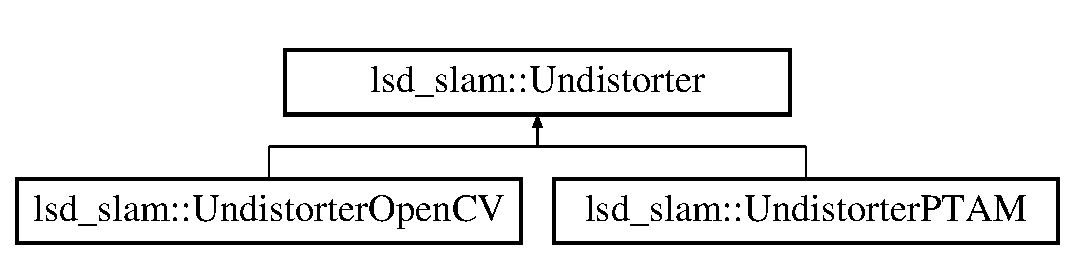
\includegraphics[height=2.000000cm]{classlsd__slam_1_1_undistorter}
\end{center}
\end{figure}
\subsection*{Public Member Functions}
\begin{DoxyCompactItemize}
\item 
virtual void \hyperlink{classlsd__slam_1_1_undistorter_a63a7b454de8e39827baf388475a013c0}{undistort} (const cv\-::\-Mat \&image, cv\-::\-Output\-Array result) const =0
\item 
virtual const cv\-::\-Mat \& \hyperlink{classlsd__slam_1_1_undistorter_ad1e2c7f6b622c6c3055fb895ba9956c4}{get\-K} () const =0
\item 
virtual const cv\-::\-Mat \& \hyperlink{classlsd__slam_1_1_undistorter_aa53850c410d84266cc682db6ab37a7a1}{get\-Original\-K} () const =0
\item 
virtual int \hyperlink{classlsd__slam_1_1_undistorter_aefaf2aec48ea920aac875c7da945efec}{get\-Output\-Width} () const =0
\item 
virtual int \hyperlink{classlsd__slam_1_1_undistorter_a72dc7d213c5fd408c586158c30578276}{get\-Output\-Height} () const =0
\item 
virtual int \hyperlink{classlsd__slam_1_1_undistorter_ad809f3b69500eae5f689a60ca766dd2e}{get\-Input\-Width} () const =0
\item 
virtual int \hyperlink{classlsd__slam_1_1_undistorter_a673e446ee77a3bbb3e934e541963612a}{get\-Input\-Height} () const =0
\item 
virtual bool \hyperlink{classlsd__slam_1_1_undistorter_a449d951327590c333da0432e6bac7b14}{is\-Valid} () const =0
\end{DoxyCompactItemize}
\subsection*{Static Public Member Functions}
\begin{DoxyCompactItemize}
\item 
static \hyperlink{classlsd__slam_1_1_undistorter}{Undistorter} $\ast$ \hyperlink{classlsd__slam_1_1_undistorter_aabd511a3c50cb169dcef290d645b00c5}{get\-Undistorter\-For\-File} (const char $\ast$config\-Filename)
\end{DoxyCompactItemize}


\subsection{Member Function Documentation}
\hypertarget{classlsd__slam_1_1_undistorter_a673e446ee77a3bbb3e934e541963612a}{\index{lsd\-\_\-slam\-::\-Undistorter@{lsd\-\_\-slam\-::\-Undistorter}!get\-Input\-Height@{get\-Input\-Height}}
\index{get\-Input\-Height@{get\-Input\-Height}!lsd_slam::Undistorter@{lsd\-\_\-slam\-::\-Undistorter}}
\subsubsection[{get\-Input\-Height}]{\setlength{\rightskip}{0pt plus 5cm}virtual int lsd\-\_\-slam\-::\-Undistorter\-::get\-Input\-Height (
\begin{DoxyParamCaption}
{}
\end{DoxyParamCaption}
) const\hspace{0.3cm}{\ttfamily [pure virtual]}}}\label{classlsd__slam_1_1_undistorter_a673e446ee77a3bbb3e934e541963612a}
Returns the height of the input images in pixels. 

Implemented in \hyperlink{classlsd__slam_1_1_undistorter_open_c_v_a0945bdec1a94a7685824cfccc583836d}{lsd\-\_\-slam\-::\-Undistorter\-Open\-C\-V}, and \hyperlink{classlsd__slam_1_1_undistorter_p_t_a_m_af63d30f057b5c9a0ca1443c5a021ec2a}{lsd\-\_\-slam\-::\-Undistorter\-P\-T\-A\-M}.

\hypertarget{classlsd__slam_1_1_undistorter_ad809f3b69500eae5f689a60ca766dd2e}{\index{lsd\-\_\-slam\-::\-Undistorter@{lsd\-\_\-slam\-::\-Undistorter}!get\-Input\-Width@{get\-Input\-Width}}
\index{get\-Input\-Width@{get\-Input\-Width}!lsd_slam::Undistorter@{lsd\-\_\-slam\-::\-Undistorter}}
\subsubsection[{get\-Input\-Width}]{\setlength{\rightskip}{0pt plus 5cm}virtual int lsd\-\_\-slam\-::\-Undistorter\-::get\-Input\-Width (
\begin{DoxyParamCaption}
{}
\end{DoxyParamCaption}
) const\hspace{0.3cm}{\ttfamily [pure virtual]}}}\label{classlsd__slam_1_1_undistorter_ad809f3b69500eae5f689a60ca766dd2e}
Returns the width of the input images in pixels. 

Implemented in \hyperlink{classlsd__slam_1_1_undistorter_open_c_v_a54404844c492185ae02bead84413297c}{lsd\-\_\-slam\-::\-Undistorter\-Open\-C\-V}, and \hyperlink{classlsd__slam_1_1_undistorter_p_t_a_m_a70e1884e007e040d2fb0eb4081fe7520}{lsd\-\_\-slam\-::\-Undistorter\-P\-T\-A\-M}.

\hypertarget{classlsd__slam_1_1_undistorter_ad1e2c7f6b622c6c3055fb895ba9956c4}{\index{lsd\-\_\-slam\-::\-Undistorter@{lsd\-\_\-slam\-::\-Undistorter}!get\-K@{get\-K}}
\index{get\-K@{get\-K}!lsd_slam::Undistorter@{lsd\-\_\-slam\-::\-Undistorter}}
\subsubsection[{get\-K}]{\setlength{\rightskip}{0pt plus 5cm}virtual const cv\-::\-Mat\& lsd\-\_\-slam\-::\-Undistorter\-::get\-K (
\begin{DoxyParamCaption}
{}
\end{DoxyParamCaption}
) const\hspace{0.3cm}{\ttfamily [pure virtual]}}}\label{classlsd__slam_1_1_undistorter_ad1e2c7f6b622c6c3055fb895ba9956c4}
Returns the intrinsic parameter matrix of the undistorted images. 

Implemented in \hyperlink{classlsd__slam_1_1_undistorter_open_c_v_a5fde19e93231ad65dbf6c98ad009c605}{lsd\-\_\-slam\-::\-Undistorter\-Open\-C\-V}, and \hyperlink{classlsd__slam_1_1_undistorter_p_t_a_m_a1a569488b001379a5e75942a3aad3a0c}{lsd\-\_\-slam\-::\-Undistorter\-P\-T\-A\-M}.

\hypertarget{classlsd__slam_1_1_undistorter_aa53850c410d84266cc682db6ab37a7a1}{\index{lsd\-\_\-slam\-::\-Undistorter@{lsd\-\_\-slam\-::\-Undistorter}!get\-Original\-K@{get\-Original\-K}}
\index{get\-Original\-K@{get\-Original\-K}!lsd_slam::Undistorter@{lsd\-\_\-slam\-::\-Undistorter}}
\subsubsection[{get\-Original\-K}]{\setlength{\rightskip}{0pt plus 5cm}virtual const cv\-::\-Mat\& lsd\-\_\-slam\-::\-Undistorter\-::get\-Original\-K (
\begin{DoxyParamCaption}
{}
\end{DoxyParamCaption}
) const\hspace{0.3cm}{\ttfamily [pure virtual]}}}\label{classlsd__slam_1_1_undistorter_aa53850c410d84266cc682db6ab37a7a1}
Returns the intrinsic parameter matrix of the original images, 

Implemented in \hyperlink{classlsd__slam_1_1_undistorter_open_c_v_ab1b18629303917c0930a41b7954a49fc}{lsd\-\_\-slam\-::\-Undistorter\-Open\-C\-V}, and \hyperlink{classlsd__slam_1_1_undistorter_p_t_a_m_a636b3b0d129929ab125bb9e2affa82c0}{lsd\-\_\-slam\-::\-Undistorter\-P\-T\-A\-M}.

\hypertarget{classlsd__slam_1_1_undistorter_a72dc7d213c5fd408c586158c30578276}{\index{lsd\-\_\-slam\-::\-Undistorter@{lsd\-\_\-slam\-::\-Undistorter}!get\-Output\-Height@{get\-Output\-Height}}
\index{get\-Output\-Height@{get\-Output\-Height}!lsd_slam::Undistorter@{lsd\-\_\-slam\-::\-Undistorter}}
\subsubsection[{get\-Output\-Height}]{\setlength{\rightskip}{0pt plus 5cm}virtual int lsd\-\_\-slam\-::\-Undistorter\-::get\-Output\-Height (
\begin{DoxyParamCaption}
{}
\end{DoxyParamCaption}
) const\hspace{0.3cm}{\ttfamily [pure virtual]}}}\label{classlsd__slam_1_1_undistorter_a72dc7d213c5fd408c586158c30578276}
Returns the height of the undistorted images in pixels. 

Implemented in \hyperlink{classlsd__slam_1_1_undistorter_open_c_v_ab6e455eb76f688d03c9159effd3ef6e2}{lsd\-\_\-slam\-::\-Undistorter\-Open\-C\-V}, and \hyperlink{classlsd__slam_1_1_undistorter_p_t_a_m_ad5c88236acc3212a3612100f5e5aacb6}{lsd\-\_\-slam\-::\-Undistorter\-P\-T\-A\-M}.

\hypertarget{classlsd__slam_1_1_undistorter_aefaf2aec48ea920aac875c7da945efec}{\index{lsd\-\_\-slam\-::\-Undistorter@{lsd\-\_\-slam\-::\-Undistorter}!get\-Output\-Width@{get\-Output\-Width}}
\index{get\-Output\-Width@{get\-Output\-Width}!lsd_slam::Undistorter@{lsd\-\_\-slam\-::\-Undistorter}}
\subsubsection[{get\-Output\-Width}]{\setlength{\rightskip}{0pt plus 5cm}virtual int lsd\-\_\-slam\-::\-Undistorter\-::get\-Output\-Width (
\begin{DoxyParamCaption}
{}
\end{DoxyParamCaption}
) const\hspace{0.3cm}{\ttfamily [pure virtual]}}}\label{classlsd__slam_1_1_undistorter_aefaf2aec48ea920aac875c7da945efec}
Returns the width of the undistorted images in pixels. 

Implemented in \hyperlink{classlsd__slam_1_1_undistorter_open_c_v_aec393d5322851339ff60b0fac92ca183}{lsd\-\_\-slam\-::\-Undistorter\-Open\-C\-V}, and \hyperlink{classlsd__slam_1_1_undistorter_p_t_a_m_a8aac80ab1305d330719e59770149ed88}{lsd\-\_\-slam\-::\-Undistorter\-P\-T\-A\-M}.

\hypertarget{classlsd__slam_1_1_undistorter_aabd511a3c50cb169dcef290d645b00c5}{\index{lsd\-\_\-slam\-::\-Undistorter@{lsd\-\_\-slam\-::\-Undistorter}!get\-Undistorter\-For\-File@{get\-Undistorter\-For\-File}}
\index{get\-Undistorter\-For\-File@{get\-Undistorter\-For\-File}!lsd_slam::Undistorter@{lsd\-\_\-slam\-::\-Undistorter}}
\subsubsection[{get\-Undistorter\-For\-File}]{\setlength{\rightskip}{0pt plus 5cm}{\bf Undistorter} $\ast$ lsd\-\_\-slam\-::\-Undistorter\-::get\-Undistorter\-For\-File (
\begin{DoxyParamCaption}
\item[{const char $\ast$}]{config\-Filename}
\end{DoxyParamCaption}
)\hspace{0.3cm}{\ttfamily [static]}}}\label{classlsd__slam_1_1_undistorter_aabd511a3c50cb169dcef290d645b00c5}
Creates and returns an \hyperlink{classlsd__slam_1_1_undistorter}{Undistorter} of the type used by the given configuration file. If the format is not recognized, returns nullptr. \hypertarget{classlsd__slam_1_1_undistorter_a449d951327590c333da0432e6bac7b14}{\index{lsd\-\_\-slam\-::\-Undistorter@{lsd\-\_\-slam\-::\-Undistorter}!is\-Valid@{is\-Valid}}
\index{is\-Valid@{is\-Valid}!lsd_slam::Undistorter@{lsd\-\_\-slam\-::\-Undistorter}}
\subsubsection[{is\-Valid}]{\setlength{\rightskip}{0pt plus 5cm}virtual bool lsd\-\_\-slam\-::\-Undistorter\-::is\-Valid (
\begin{DoxyParamCaption}
{}
\end{DoxyParamCaption}
) const\hspace{0.3cm}{\ttfamily [pure virtual]}}}\label{classlsd__slam_1_1_undistorter_a449d951327590c333da0432e6bac7b14}
Returns if the undistorter was initialized successfully. 

Implemented in \hyperlink{classlsd__slam_1_1_undistorter_open_c_v_a16603612fa9dce55c0715a19d14df0d8}{lsd\-\_\-slam\-::\-Undistorter\-Open\-C\-V}, and \hyperlink{classlsd__slam_1_1_undistorter_p_t_a_m_a80d17a49a43a574d19faf26f07acce60}{lsd\-\_\-slam\-::\-Undistorter\-P\-T\-A\-M}.

\hypertarget{classlsd__slam_1_1_undistorter_a63a7b454de8e39827baf388475a013c0}{\index{lsd\-\_\-slam\-::\-Undistorter@{lsd\-\_\-slam\-::\-Undistorter}!undistort@{undistort}}
\index{undistort@{undistort}!lsd_slam::Undistorter@{lsd\-\_\-slam\-::\-Undistorter}}
\subsubsection[{undistort}]{\setlength{\rightskip}{0pt plus 5cm}virtual void lsd\-\_\-slam\-::\-Undistorter\-::undistort (
\begin{DoxyParamCaption}
\item[{const cv\-::\-Mat \&}]{image, }
\item[{cv\-::\-Output\-Array}]{result}
\end{DoxyParamCaption}
) const\hspace{0.3cm}{\ttfamily [pure virtual]}}}\label{classlsd__slam_1_1_undistorter_a63a7b454de8e39827baf388475a013c0}
Undistorts the given image and returns the result image. 

Implemented in \hyperlink{classlsd__slam_1_1_undistorter_open_c_v_ae788f7b44d7f5760a88bcfc24fe880b4}{lsd\-\_\-slam\-::\-Undistorter\-Open\-C\-V}, and \hyperlink{classlsd__slam_1_1_undistorter_p_t_a_m_a1e74aaffa5269b0b551d05b60419fdab}{lsd\-\_\-slam\-::\-Undistorter\-P\-T\-A\-M}.



The documentation for this class was generated from the following files\-:\begin{DoxyCompactItemize}
\item 
/home/king/rgbd-\/slam-\/lets-\/do-\/it/9-\/doxygen/lsd\-\_\-slam/lsd\-\_\-slam\-\_\-core/src/util/Undistorter.\-h\item 
/home/king/rgbd-\/slam-\/lets-\/do-\/it/9-\/doxygen/lsd\-\_\-slam/lsd\-\_\-slam\-\_\-core/src/util/Undistorter.\-cpp\end{DoxyCompactItemize}

\hypertarget{classlsd__slam_1_1_undistorter_open_c_v}{\section{lsd\-\_\-slam\-:\-:Undistorter\-Open\-C\-V Class Reference}
\label{classlsd__slam_1_1_undistorter_open_c_v}\index{lsd\-\_\-slam\-::\-Undistorter\-Open\-C\-V@{lsd\-\_\-slam\-::\-Undistorter\-Open\-C\-V}}
}
Inheritance diagram for lsd\-\_\-slam\-:\-:Undistorter\-Open\-C\-V\-:\begin{figure}[H]
\begin{center}
\leavevmode
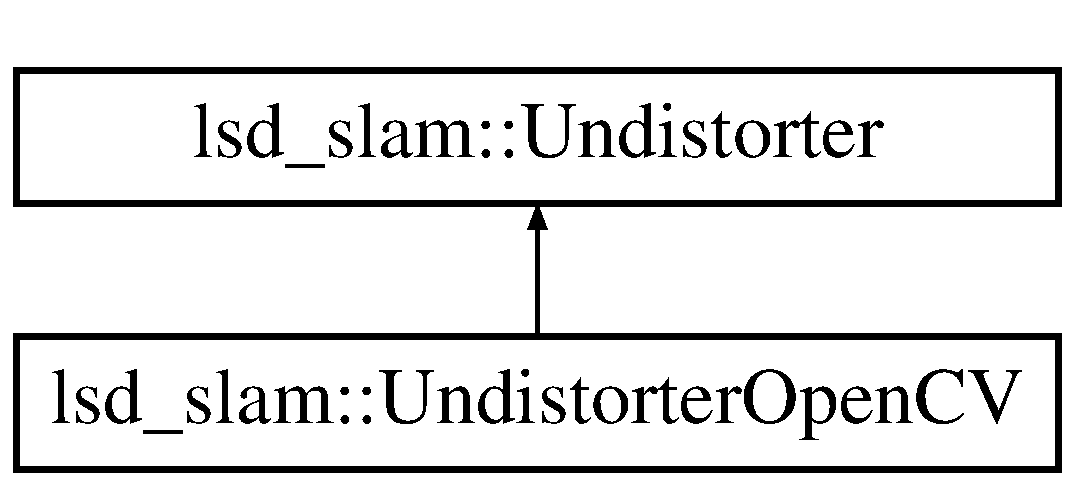
\includegraphics[height=2.000000cm]{classlsd__slam_1_1_undistorter_open_c_v}
\end{center}
\end{figure}
\subsection*{Public Member Functions}
\begin{DoxyCompactItemize}
\item 
\hyperlink{classlsd__slam_1_1_undistorter_open_c_v_afb1fc6fe47e68f31cb7ae7d696b72e4d}{Undistorter\-Open\-C\-V} (const char $\ast$config\-File\-Name)
\item 
\hyperlink{classlsd__slam_1_1_undistorter_open_c_v_a95f7331ff5c0cdd09f52a673884998df}{$\sim$\-Undistorter\-Open\-C\-V} ()
\item 
\hypertarget{classlsd__slam_1_1_undistorter_open_c_v_aedd049060155bbaab049a00c99716daa}{{\bfseries Undistorter\-Open\-C\-V} (const \hyperlink{classlsd__slam_1_1_undistorter_open_c_v}{Undistorter\-Open\-C\-V} \&)=delete}\label{classlsd__slam_1_1_undistorter_open_c_v_aedd049060155bbaab049a00c99716daa}

\item 
\hypertarget{classlsd__slam_1_1_undistorter_open_c_v_a459d3ea80c285f33a8fa236c3a7e0f32}{\hyperlink{classlsd__slam_1_1_undistorter_open_c_v}{Undistorter\-Open\-C\-V} \& {\bfseries operator=} (const \hyperlink{classlsd__slam_1_1_undistorter_open_c_v}{Undistorter\-Open\-C\-V} \&)=delete}\label{classlsd__slam_1_1_undistorter_open_c_v_a459d3ea80c285f33a8fa236c3a7e0f32}

\item 
void \hyperlink{classlsd__slam_1_1_undistorter_open_c_v_ae788f7b44d7f5760a88bcfc24fe880b4}{undistort} (const cv\-::\-Mat \&image, cv\-::\-Output\-Array result) const 
\item 
const cv\-::\-Mat \& \hyperlink{classlsd__slam_1_1_undistorter_open_c_v_a5fde19e93231ad65dbf6c98ad009c605}{get\-K} () const 
\item 
const cv\-::\-Mat \& \hyperlink{classlsd__slam_1_1_undistorter_open_c_v_ab1b18629303917c0930a41b7954a49fc}{get\-Original\-K} () const 
\item 
int \hyperlink{classlsd__slam_1_1_undistorter_open_c_v_aec393d5322851339ff60b0fac92ca183}{get\-Output\-Width} () const 
\item 
int \hyperlink{classlsd__slam_1_1_undistorter_open_c_v_ab6e455eb76f688d03c9159effd3ef6e2}{get\-Output\-Height} () const 
\item 
int \hyperlink{classlsd__slam_1_1_undistorter_open_c_v_a54404844c492185ae02bead84413297c}{get\-Input\-Width} () const 
\item 
int \hyperlink{classlsd__slam_1_1_undistorter_open_c_v_a0945bdec1a94a7685824cfccc583836d}{get\-Input\-Height} () const 
\item 
bool \hyperlink{classlsd__slam_1_1_undistorter_open_c_v_a16603612fa9dce55c0715a19d14df0d8}{is\-Valid} () const 
\end{DoxyCompactItemize}
\subsection*{Additional Inherited Members}


\subsection{Constructor \& Destructor Documentation}
\hypertarget{classlsd__slam_1_1_undistorter_open_c_v_afb1fc6fe47e68f31cb7ae7d696b72e4d}{\index{lsd\-\_\-slam\-::\-Undistorter\-Open\-C\-V@{lsd\-\_\-slam\-::\-Undistorter\-Open\-C\-V}!Undistorter\-Open\-C\-V@{Undistorter\-Open\-C\-V}}
\index{Undistorter\-Open\-C\-V@{Undistorter\-Open\-C\-V}!lsd_slam::UndistorterOpenCV@{lsd\-\_\-slam\-::\-Undistorter\-Open\-C\-V}}
\subsubsection[{Undistorter\-Open\-C\-V}]{\setlength{\rightskip}{0pt plus 5cm}lsd\-\_\-slam\-::\-Undistorter\-Open\-C\-V\-::\-Undistorter\-Open\-C\-V (
\begin{DoxyParamCaption}
\item[{const char $\ast$}]{config\-File\-Name}
\end{DoxyParamCaption}
)}}\label{classlsd__slam_1_1_undistorter_open_c_v_afb1fc6fe47e68f31cb7ae7d696b72e4d}
Creates an \hyperlink{classlsd__slam_1_1_undistorter}{Undistorter} by reading the distortion parameters from a file.

The file format is as follows\-: fx fy cx cy d1 d2 d3 d4 d5 d6 input\-Width input\-Height crop / full / none output\-Width output\-Height \hypertarget{classlsd__slam_1_1_undistorter_open_c_v_a95f7331ff5c0cdd09f52a673884998df}{\index{lsd\-\_\-slam\-::\-Undistorter\-Open\-C\-V@{lsd\-\_\-slam\-::\-Undistorter\-Open\-C\-V}!$\sim$\-Undistorter\-Open\-C\-V@{$\sim$\-Undistorter\-Open\-C\-V}}
\index{$\sim$\-Undistorter\-Open\-C\-V@{$\sim$\-Undistorter\-Open\-C\-V}!lsd_slam::UndistorterOpenCV@{lsd\-\_\-slam\-::\-Undistorter\-Open\-C\-V}}
\subsubsection[{$\sim$\-Undistorter\-Open\-C\-V}]{\setlength{\rightskip}{0pt plus 5cm}lsd\-\_\-slam\-::\-Undistorter\-Open\-C\-V\-::$\sim$\-Undistorter\-Open\-C\-V (
\begin{DoxyParamCaption}
{}
\end{DoxyParamCaption}
)}}\label{classlsd__slam_1_1_undistorter_open_c_v_a95f7331ff5c0cdd09f52a673884998df}
Destructor. 

\subsection{Member Function Documentation}
\hypertarget{classlsd__slam_1_1_undistorter_open_c_v_a0945bdec1a94a7685824cfccc583836d}{\index{lsd\-\_\-slam\-::\-Undistorter\-Open\-C\-V@{lsd\-\_\-slam\-::\-Undistorter\-Open\-C\-V}!get\-Input\-Height@{get\-Input\-Height}}
\index{get\-Input\-Height@{get\-Input\-Height}!lsd_slam::UndistorterOpenCV@{lsd\-\_\-slam\-::\-Undistorter\-Open\-C\-V}}
\subsubsection[{get\-Input\-Height}]{\setlength{\rightskip}{0pt plus 5cm}int lsd\-\_\-slam\-::\-Undistorter\-Open\-C\-V\-::get\-Input\-Height (
\begin{DoxyParamCaption}
{}
\end{DoxyParamCaption}
) const\hspace{0.3cm}{\ttfamily [virtual]}}}\label{classlsd__slam_1_1_undistorter_open_c_v_a0945bdec1a94a7685824cfccc583836d}
Returns the height of the input images in pixels. 

Implements \hyperlink{classlsd__slam_1_1_undistorter_a673e446ee77a3bbb3e934e541963612a}{lsd\-\_\-slam\-::\-Undistorter}.

\hypertarget{classlsd__slam_1_1_undistorter_open_c_v_a54404844c492185ae02bead84413297c}{\index{lsd\-\_\-slam\-::\-Undistorter\-Open\-C\-V@{lsd\-\_\-slam\-::\-Undistorter\-Open\-C\-V}!get\-Input\-Width@{get\-Input\-Width}}
\index{get\-Input\-Width@{get\-Input\-Width}!lsd_slam::UndistorterOpenCV@{lsd\-\_\-slam\-::\-Undistorter\-Open\-C\-V}}
\subsubsection[{get\-Input\-Width}]{\setlength{\rightskip}{0pt plus 5cm}int lsd\-\_\-slam\-::\-Undistorter\-Open\-C\-V\-::get\-Input\-Width (
\begin{DoxyParamCaption}
{}
\end{DoxyParamCaption}
) const\hspace{0.3cm}{\ttfamily [virtual]}}}\label{classlsd__slam_1_1_undistorter_open_c_v_a54404844c492185ae02bead84413297c}
Returns the width of the input images in pixels. 

Implements \hyperlink{classlsd__slam_1_1_undistorter_ad809f3b69500eae5f689a60ca766dd2e}{lsd\-\_\-slam\-::\-Undistorter}.

\hypertarget{classlsd__slam_1_1_undistorter_open_c_v_a5fde19e93231ad65dbf6c98ad009c605}{\index{lsd\-\_\-slam\-::\-Undistorter\-Open\-C\-V@{lsd\-\_\-slam\-::\-Undistorter\-Open\-C\-V}!get\-K@{get\-K}}
\index{get\-K@{get\-K}!lsd_slam::UndistorterOpenCV@{lsd\-\_\-slam\-::\-Undistorter\-Open\-C\-V}}
\subsubsection[{get\-K}]{\setlength{\rightskip}{0pt plus 5cm}const cv\-::\-Mat \& lsd\-\_\-slam\-::\-Undistorter\-Open\-C\-V\-::get\-K (
\begin{DoxyParamCaption}
{}
\end{DoxyParamCaption}
) const\hspace{0.3cm}{\ttfamily [virtual]}}}\label{classlsd__slam_1_1_undistorter_open_c_v_a5fde19e93231ad65dbf6c98ad009c605}
Returns the intrinsic parameter matrix of the undistorted images. 

Implements \hyperlink{classlsd__slam_1_1_undistorter_ad1e2c7f6b622c6c3055fb895ba9956c4}{lsd\-\_\-slam\-::\-Undistorter}.

\hypertarget{classlsd__slam_1_1_undistorter_open_c_v_ab1b18629303917c0930a41b7954a49fc}{\index{lsd\-\_\-slam\-::\-Undistorter\-Open\-C\-V@{lsd\-\_\-slam\-::\-Undistorter\-Open\-C\-V}!get\-Original\-K@{get\-Original\-K}}
\index{get\-Original\-K@{get\-Original\-K}!lsd_slam::UndistorterOpenCV@{lsd\-\_\-slam\-::\-Undistorter\-Open\-C\-V}}
\subsubsection[{get\-Original\-K}]{\setlength{\rightskip}{0pt plus 5cm}const cv\-::\-Mat \& lsd\-\_\-slam\-::\-Undistorter\-Open\-C\-V\-::get\-Original\-K (
\begin{DoxyParamCaption}
{}
\end{DoxyParamCaption}
) const\hspace{0.3cm}{\ttfamily [virtual]}}}\label{classlsd__slam_1_1_undistorter_open_c_v_ab1b18629303917c0930a41b7954a49fc}
Returns the intrinsic parameter matrix of the original images, 

Implements \hyperlink{classlsd__slam_1_1_undistorter_aa53850c410d84266cc682db6ab37a7a1}{lsd\-\_\-slam\-::\-Undistorter}.

\hypertarget{classlsd__slam_1_1_undistorter_open_c_v_ab6e455eb76f688d03c9159effd3ef6e2}{\index{lsd\-\_\-slam\-::\-Undistorter\-Open\-C\-V@{lsd\-\_\-slam\-::\-Undistorter\-Open\-C\-V}!get\-Output\-Height@{get\-Output\-Height}}
\index{get\-Output\-Height@{get\-Output\-Height}!lsd_slam::UndistorterOpenCV@{lsd\-\_\-slam\-::\-Undistorter\-Open\-C\-V}}
\subsubsection[{get\-Output\-Height}]{\setlength{\rightskip}{0pt plus 5cm}int lsd\-\_\-slam\-::\-Undistorter\-Open\-C\-V\-::get\-Output\-Height (
\begin{DoxyParamCaption}
{}
\end{DoxyParamCaption}
) const\hspace{0.3cm}{\ttfamily [virtual]}}}\label{classlsd__slam_1_1_undistorter_open_c_v_ab6e455eb76f688d03c9159effd3ef6e2}
Returns the height of the undistorted images in pixels. 

Implements \hyperlink{classlsd__slam_1_1_undistorter_a72dc7d213c5fd408c586158c30578276}{lsd\-\_\-slam\-::\-Undistorter}.

\hypertarget{classlsd__slam_1_1_undistorter_open_c_v_aec393d5322851339ff60b0fac92ca183}{\index{lsd\-\_\-slam\-::\-Undistorter\-Open\-C\-V@{lsd\-\_\-slam\-::\-Undistorter\-Open\-C\-V}!get\-Output\-Width@{get\-Output\-Width}}
\index{get\-Output\-Width@{get\-Output\-Width}!lsd_slam::UndistorterOpenCV@{lsd\-\_\-slam\-::\-Undistorter\-Open\-C\-V}}
\subsubsection[{get\-Output\-Width}]{\setlength{\rightskip}{0pt plus 5cm}int lsd\-\_\-slam\-::\-Undistorter\-Open\-C\-V\-::get\-Output\-Width (
\begin{DoxyParamCaption}
{}
\end{DoxyParamCaption}
) const\hspace{0.3cm}{\ttfamily [virtual]}}}\label{classlsd__slam_1_1_undistorter_open_c_v_aec393d5322851339ff60b0fac92ca183}
Returns the width of the undistorted images in pixels. 

Implements \hyperlink{classlsd__slam_1_1_undistorter_aefaf2aec48ea920aac875c7da945efec}{lsd\-\_\-slam\-::\-Undistorter}.

\hypertarget{classlsd__slam_1_1_undistorter_open_c_v_a16603612fa9dce55c0715a19d14df0d8}{\index{lsd\-\_\-slam\-::\-Undistorter\-Open\-C\-V@{lsd\-\_\-slam\-::\-Undistorter\-Open\-C\-V}!is\-Valid@{is\-Valid}}
\index{is\-Valid@{is\-Valid}!lsd_slam::UndistorterOpenCV@{lsd\-\_\-slam\-::\-Undistorter\-Open\-C\-V}}
\subsubsection[{is\-Valid}]{\setlength{\rightskip}{0pt plus 5cm}bool lsd\-\_\-slam\-::\-Undistorter\-Open\-C\-V\-::is\-Valid (
\begin{DoxyParamCaption}
{}
\end{DoxyParamCaption}
) const\hspace{0.3cm}{\ttfamily [virtual]}}}\label{classlsd__slam_1_1_undistorter_open_c_v_a16603612fa9dce55c0715a19d14df0d8}
Returns if the undistorter was initialized successfully. 

Implements \hyperlink{classlsd__slam_1_1_undistorter_a449d951327590c333da0432e6bac7b14}{lsd\-\_\-slam\-::\-Undistorter}.

\hypertarget{classlsd__slam_1_1_undistorter_open_c_v_ae788f7b44d7f5760a88bcfc24fe880b4}{\index{lsd\-\_\-slam\-::\-Undistorter\-Open\-C\-V@{lsd\-\_\-slam\-::\-Undistorter\-Open\-C\-V}!undistort@{undistort}}
\index{undistort@{undistort}!lsd_slam::UndistorterOpenCV@{lsd\-\_\-slam\-::\-Undistorter\-Open\-C\-V}}
\subsubsection[{undistort}]{\setlength{\rightskip}{0pt plus 5cm}void lsd\-\_\-slam\-::\-Undistorter\-Open\-C\-V\-::undistort (
\begin{DoxyParamCaption}
\item[{const cv\-::\-Mat \&}]{image, }
\item[{cv\-::\-Output\-Array}]{result}
\end{DoxyParamCaption}
) const\hspace{0.3cm}{\ttfamily [virtual]}}}\label{classlsd__slam_1_1_undistorter_open_c_v_ae788f7b44d7f5760a88bcfc24fe880b4}
Undistorts the given image and returns the result image. 

Implements \hyperlink{classlsd__slam_1_1_undistorter_a63a7b454de8e39827baf388475a013c0}{lsd\-\_\-slam\-::\-Undistorter}.



The documentation for this class was generated from the following files\-:\begin{DoxyCompactItemize}
\item 
/home/king/rgbd-\/slam-\/lets-\/do-\/it/9-\/doxygen/lsd\-\_\-slam/lsd\-\_\-slam\-\_\-core/src/util/Undistorter.\-h\item 
/home/king/rgbd-\/slam-\/lets-\/do-\/it/9-\/doxygen/lsd\-\_\-slam/lsd\-\_\-slam\-\_\-core/src/util/Undistorter.\-cpp\end{DoxyCompactItemize}

\hypertarget{classlsd__slam_1_1_undistorter_p_t_a_m}{\section{lsd\-\_\-slam\-:\-:Undistorter\-P\-T\-A\-M Class Reference}
\label{classlsd__slam_1_1_undistorter_p_t_a_m}\index{lsd\-\_\-slam\-::\-Undistorter\-P\-T\-A\-M@{lsd\-\_\-slam\-::\-Undistorter\-P\-T\-A\-M}}
}
Inheritance diagram for lsd\-\_\-slam\-:\-:Undistorter\-P\-T\-A\-M\-:\begin{figure}[H]
\begin{center}
\leavevmode
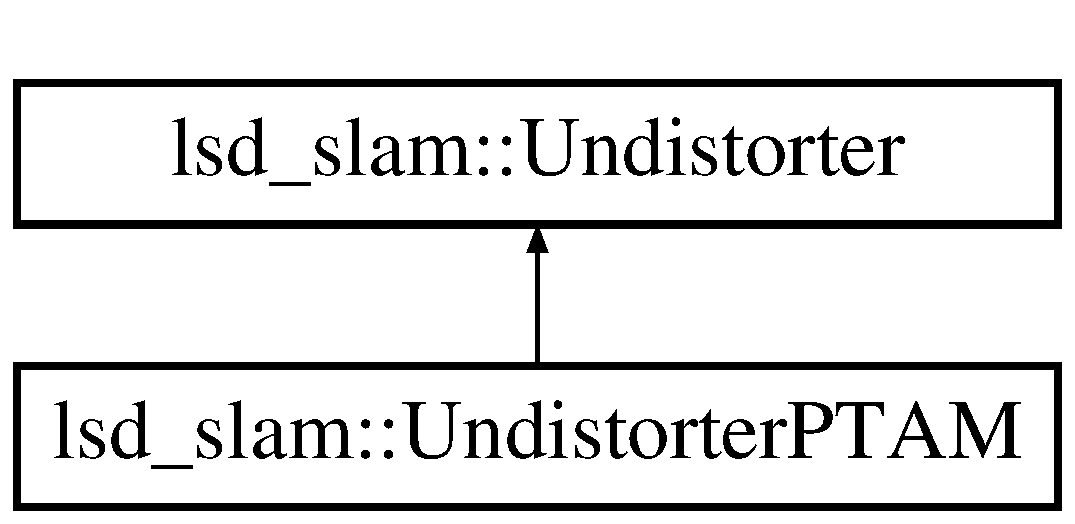
\includegraphics[height=2.000000cm]{classlsd__slam_1_1_undistorter_p_t_a_m}
\end{center}
\end{figure}
\subsection*{Public Member Functions}
\begin{DoxyCompactItemize}
\item 
\hyperlink{classlsd__slam_1_1_undistorter_p_t_a_m_ac7604cab28f1987264f0da123bcc990a}{Undistorter\-P\-T\-A\-M} (const char $\ast$config\-File\-Name)
\item 
\hyperlink{classlsd__slam_1_1_undistorter_p_t_a_m_aa24a3a52c7515c04c503a33a55db2a9b}{$\sim$\-Undistorter\-P\-T\-A\-M} ()
\item 
\hypertarget{classlsd__slam_1_1_undistorter_p_t_a_m_a13fe7f2773c8fc5a901a7249fd671b93}{{\bfseries Undistorter\-P\-T\-A\-M} (const \hyperlink{classlsd__slam_1_1_undistorter_p_t_a_m}{Undistorter\-P\-T\-A\-M} \&)=delete}\label{classlsd__slam_1_1_undistorter_p_t_a_m_a13fe7f2773c8fc5a901a7249fd671b93}

\item 
\hypertarget{classlsd__slam_1_1_undistorter_p_t_a_m_a8ede83714decea8c7af0a3ebcb1b599f}{\hyperlink{classlsd__slam_1_1_undistorter_p_t_a_m}{Undistorter\-P\-T\-A\-M} \& {\bfseries operator=} (const \hyperlink{classlsd__slam_1_1_undistorter_p_t_a_m}{Undistorter\-P\-T\-A\-M} \&)=delete}\label{classlsd__slam_1_1_undistorter_p_t_a_m_a8ede83714decea8c7af0a3ebcb1b599f}

\item 
void \hyperlink{classlsd__slam_1_1_undistorter_p_t_a_m_a1e74aaffa5269b0b551d05b60419fdab}{undistort} (const cv\-::\-Mat \&image, cv\-::\-Output\-Array result) const 
\item 
const cv\-::\-Mat \& \hyperlink{classlsd__slam_1_1_undistorter_p_t_a_m_a1a569488b001379a5e75942a3aad3a0c}{get\-K} () const 
\item 
const cv\-::\-Mat \& \hyperlink{classlsd__slam_1_1_undistorter_p_t_a_m_a636b3b0d129929ab125bb9e2affa82c0}{get\-Original\-K} () const 
\item 
int \hyperlink{classlsd__slam_1_1_undistorter_p_t_a_m_a8aac80ab1305d330719e59770149ed88}{get\-Output\-Width} () const 
\item 
int \hyperlink{classlsd__slam_1_1_undistorter_p_t_a_m_ad5c88236acc3212a3612100f5e5aacb6}{get\-Output\-Height} () const 
\item 
int \hyperlink{classlsd__slam_1_1_undistorter_p_t_a_m_a70e1884e007e040d2fb0eb4081fe7520}{get\-Input\-Width} () const 
\item 
int \hyperlink{classlsd__slam_1_1_undistorter_p_t_a_m_af63d30f057b5c9a0ca1443c5a021ec2a}{get\-Input\-Height} () const 
\item 
bool \hyperlink{classlsd__slam_1_1_undistorter_p_t_a_m_a80d17a49a43a574d19faf26f07acce60}{is\-Valid} () const 
\end{DoxyCompactItemize}
\subsection*{Additional Inherited Members}


\subsection{Constructor \& Destructor Documentation}
\hypertarget{classlsd__slam_1_1_undistorter_p_t_a_m_ac7604cab28f1987264f0da123bcc990a}{\index{lsd\-\_\-slam\-::\-Undistorter\-P\-T\-A\-M@{lsd\-\_\-slam\-::\-Undistorter\-P\-T\-A\-M}!Undistorter\-P\-T\-A\-M@{Undistorter\-P\-T\-A\-M}}
\index{Undistorter\-P\-T\-A\-M@{Undistorter\-P\-T\-A\-M}!lsd_slam::UndistorterPTAM@{lsd\-\_\-slam\-::\-Undistorter\-P\-T\-A\-M}}
\subsubsection[{Undistorter\-P\-T\-A\-M}]{\setlength{\rightskip}{0pt plus 5cm}lsd\-\_\-slam\-::\-Undistorter\-P\-T\-A\-M\-::\-Undistorter\-P\-T\-A\-M (
\begin{DoxyParamCaption}
\item[{const char $\ast$}]{config\-File\-Name}
\end{DoxyParamCaption}
)}}\label{classlsd__slam_1_1_undistorter_p_t_a_m_ac7604cab28f1987264f0da123bcc990a}
Creates an \hyperlink{classlsd__slam_1_1_undistorter}{Undistorter} by reading the distortion parameters from a file.

The file format is as follows\-: d1 d2 d3 d4 d5 input\-Width input\-Height crop / full / none output\-Width output\-Height \hypertarget{classlsd__slam_1_1_undistorter_p_t_a_m_aa24a3a52c7515c04c503a33a55db2a9b}{\index{lsd\-\_\-slam\-::\-Undistorter\-P\-T\-A\-M@{lsd\-\_\-slam\-::\-Undistorter\-P\-T\-A\-M}!$\sim$\-Undistorter\-P\-T\-A\-M@{$\sim$\-Undistorter\-P\-T\-A\-M}}
\index{$\sim$\-Undistorter\-P\-T\-A\-M@{$\sim$\-Undistorter\-P\-T\-A\-M}!lsd_slam::UndistorterPTAM@{lsd\-\_\-slam\-::\-Undistorter\-P\-T\-A\-M}}
\subsubsection[{$\sim$\-Undistorter\-P\-T\-A\-M}]{\setlength{\rightskip}{0pt plus 5cm}lsd\-\_\-slam\-::\-Undistorter\-P\-T\-A\-M\-::$\sim$\-Undistorter\-P\-T\-A\-M (
\begin{DoxyParamCaption}
{}
\end{DoxyParamCaption}
)}}\label{classlsd__slam_1_1_undistorter_p_t_a_m_aa24a3a52c7515c04c503a33a55db2a9b}
Destructor. 

\subsection{Member Function Documentation}
\hypertarget{classlsd__slam_1_1_undistorter_p_t_a_m_af63d30f057b5c9a0ca1443c5a021ec2a}{\index{lsd\-\_\-slam\-::\-Undistorter\-P\-T\-A\-M@{lsd\-\_\-slam\-::\-Undistorter\-P\-T\-A\-M}!get\-Input\-Height@{get\-Input\-Height}}
\index{get\-Input\-Height@{get\-Input\-Height}!lsd_slam::UndistorterPTAM@{lsd\-\_\-slam\-::\-Undistorter\-P\-T\-A\-M}}
\subsubsection[{get\-Input\-Height}]{\setlength{\rightskip}{0pt plus 5cm}int lsd\-\_\-slam\-::\-Undistorter\-P\-T\-A\-M\-::get\-Input\-Height (
\begin{DoxyParamCaption}
{}
\end{DoxyParamCaption}
) const\hspace{0.3cm}{\ttfamily [virtual]}}}\label{classlsd__slam_1_1_undistorter_p_t_a_m_af63d30f057b5c9a0ca1443c5a021ec2a}
Returns the height of the input images in pixels. 

Implements \hyperlink{classlsd__slam_1_1_undistorter_a673e446ee77a3bbb3e934e541963612a}{lsd\-\_\-slam\-::\-Undistorter}.

\hypertarget{classlsd__slam_1_1_undistorter_p_t_a_m_a70e1884e007e040d2fb0eb4081fe7520}{\index{lsd\-\_\-slam\-::\-Undistorter\-P\-T\-A\-M@{lsd\-\_\-slam\-::\-Undistorter\-P\-T\-A\-M}!get\-Input\-Width@{get\-Input\-Width}}
\index{get\-Input\-Width@{get\-Input\-Width}!lsd_slam::UndistorterPTAM@{lsd\-\_\-slam\-::\-Undistorter\-P\-T\-A\-M}}
\subsubsection[{get\-Input\-Width}]{\setlength{\rightskip}{0pt plus 5cm}int lsd\-\_\-slam\-::\-Undistorter\-P\-T\-A\-M\-::get\-Input\-Width (
\begin{DoxyParamCaption}
{}
\end{DoxyParamCaption}
) const\hspace{0.3cm}{\ttfamily [virtual]}}}\label{classlsd__slam_1_1_undistorter_p_t_a_m_a70e1884e007e040d2fb0eb4081fe7520}
Returns the width of the input images in pixels. 

Implements \hyperlink{classlsd__slam_1_1_undistorter_ad809f3b69500eae5f689a60ca766dd2e}{lsd\-\_\-slam\-::\-Undistorter}.

\hypertarget{classlsd__slam_1_1_undistorter_p_t_a_m_a1a569488b001379a5e75942a3aad3a0c}{\index{lsd\-\_\-slam\-::\-Undistorter\-P\-T\-A\-M@{lsd\-\_\-slam\-::\-Undistorter\-P\-T\-A\-M}!get\-K@{get\-K}}
\index{get\-K@{get\-K}!lsd_slam::UndistorterPTAM@{lsd\-\_\-slam\-::\-Undistorter\-P\-T\-A\-M}}
\subsubsection[{get\-K}]{\setlength{\rightskip}{0pt plus 5cm}const cv\-::\-Mat \& lsd\-\_\-slam\-::\-Undistorter\-P\-T\-A\-M\-::get\-K (
\begin{DoxyParamCaption}
{}
\end{DoxyParamCaption}
) const\hspace{0.3cm}{\ttfamily [virtual]}}}\label{classlsd__slam_1_1_undistorter_p_t_a_m_a1a569488b001379a5e75942a3aad3a0c}
Returns the intrinsic parameter matrix of the undistorted images. 

Implements \hyperlink{classlsd__slam_1_1_undistorter_ad1e2c7f6b622c6c3055fb895ba9956c4}{lsd\-\_\-slam\-::\-Undistorter}.

\hypertarget{classlsd__slam_1_1_undistorter_p_t_a_m_a636b3b0d129929ab125bb9e2affa82c0}{\index{lsd\-\_\-slam\-::\-Undistorter\-P\-T\-A\-M@{lsd\-\_\-slam\-::\-Undistorter\-P\-T\-A\-M}!get\-Original\-K@{get\-Original\-K}}
\index{get\-Original\-K@{get\-Original\-K}!lsd_slam::UndistorterPTAM@{lsd\-\_\-slam\-::\-Undistorter\-P\-T\-A\-M}}
\subsubsection[{get\-Original\-K}]{\setlength{\rightskip}{0pt plus 5cm}const cv\-::\-Mat \& lsd\-\_\-slam\-::\-Undistorter\-P\-T\-A\-M\-::get\-Original\-K (
\begin{DoxyParamCaption}
{}
\end{DoxyParamCaption}
) const\hspace{0.3cm}{\ttfamily [virtual]}}}\label{classlsd__slam_1_1_undistorter_p_t_a_m_a636b3b0d129929ab125bb9e2affa82c0}
Returns the intrinsic parameter matrix of the original images, 

Implements \hyperlink{classlsd__slam_1_1_undistorter_aa53850c410d84266cc682db6ab37a7a1}{lsd\-\_\-slam\-::\-Undistorter}.

\hypertarget{classlsd__slam_1_1_undistorter_p_t_a_m_ad5c88236acc3212a3612100f5e5aacb6}{\index{lsd\-\_\-slam\-::\-Undistorter\-P\-T\-A\-M@{lsd\-\_\-slam\-::\-Undistorter\-P\-T\-A\-M}!get\-Output\-Height@{get\-Output\-Height}}
\index{get\-Output\-Height@{get\-Output\-Height}!lsd_slam::UndistorterPTAM@{lsd\-\_\-slam\-::\-Undistorter\-P\-T\-A\-M}}
\subsubsection[{get\-Output\-Height}]{\setlength{\rightskip}{0pt plus 5cm}int lsd\-\_\-slam\-::\-Undistorter\-P\-T\-A\-M\-::get\-Output\-Height (
\begin{DoxyParamCaption}
{}
\end{DoxyParamCaption}
) const\hspace{0.3cm}{\ttfamily [virtual]}}}\label{classlsd__slam_1_1_undistorter_p_t_a_m_ad5c88236acc3212a3612100f5e5aacb6}
Returns the height of the undistorted images in pixels. 

Implements \hyperlink{classlsd__slam_1_1_undistorter_a72dc7d213c5fd408c586158c30578276}{lsd\-\_\-slam\-::\-Undistorter}.

\hypertarget{classlsd__slam_1_1_undistorter_p_t_a_m_a8aac80ab1305d330719e59770149ed88}{\index{lsd\-\_\-slam\-::\-Undistorter\-P\-T\-A\-M@{lsd\-\_\-slam\-::\-Undistorter\-P\-T\-A\-M}!get\-Output\-Width@{get\-Output\-Width}}
\index{get\-Output\-Width@{get\-Output\-Width}!lsd_slam::UndistorterPTAM@{lsd\-\_\-slam\-::\-Undistorter\-P\-T\-A\-M}}
\subsubsection[{get\-Output\-Width}]{\setlength{\rightskip}{0pt plus 5cm}int lsd\-\_\-slam\-::\-Undistorter\-P\-T\-A\-M\-::get\-Output\-Width (
\begin{DoxyParamCaption}
{}
\end{DoxyParamCaption}
) const\hspace{0.3cm}{\ttfamily [virtual]}}}\label{classlsd__slam_1_1_undistorter_p_t_a_m_a8aac80ab1305d330719e59770149ed88}
Returns the width of the undistorted images in pixels. 

Implements \hyperlink{classlsd__slam_1_1_undistorter_aefaf2aec48ea920aac875c7da945efec}{lsd\-\_\-slam\-::\-Undistorter}.

\hypertarget{classlsd__slam_1_1_undistorter_p_t_a_m_a80d17a49a43a574d19faf26f07acce60}{\index{lsd\-\_\-slam\-::\-Undistorter\-P\-T\-A\-M@{lsd\-\_\-slam\-::\-Undistorter\-P\-T\-A\-M}!is\-Valid@{is\-Valid}}
\index{is\-Valid@{is\-Valid}!lsd_slam::UndistorterPTAM@{lsd\-\_\-slam\-::\-Undistorter\-P\-T\-A\-M}}
\subsubsection[{is\-Valid}]{\setlength{\rightskip}{0pt plus 5cm}bool lsd\-\_\-slam\-::\-Undistorter\-P\-T\-A\-M\-::is\-Valid (
\begin{DoxyParamCaption}
{}
\end{DoxyParamCaption}
) const\hspace{0.3cm}{\ttfamily [virtual]}}}\label{classlsd__slam_1_1_undistorter_p_t_a_m_a80d17a49a43a574d19faf26f07acce60}
Returns if the undistorter was initialized successfully. 

Implements \hyperlink{classlsd__slam_1_1_undistorter_a449d951327590c333da0432e6bac7b14}{lsd\-\_\-slam\-::\-Undistorter}.

\hypertarget{classlsd__slam_1_1_undistorter_p_t_a_m_a1e74aaffa5269b0b551d05b60419fdab}{\index{lsd\-\_\-slam\-::\-Undistorter\-P\-T\-A\-M@{lsd\-\_\-slam\-::\-Undistorter\-P\-T\-A\-M}!undistort@{undistort}}
\index{undistort@{undistort}!lsd_slam::UndistorterPTAM@{lsd\-\_\-slam\-::\-Undistorter\-P\-T\-A\-M}}
\subsubsection[{undistort}]{\setlength{\rightskip}{0pt plus 5cm}void lsd\-\_\-slam\-::\-Undistorter\-P\-T\-A\-M\-::undistort (
\begin{DoxyParamCaption}
\item[{const cv\-::\-Mat \&}]{image, }
\item[{cv\-::\-Output\-Array}]{result}
\end{DoxyParamCaption}
) const\hspace{0.3cm}{\ttfamily [virtual]}}}\label{classlsd__slam_1_1_undistorter_p_t_a_m_a1e74aaffa5269b0b551d05b60419fdab}
Undistorts the given image and returns the result image. 

Implements \hyperlink{classlsd__slam_1_1_undistorter_a63a7b454de8e39827baf388475a013c0}{lsd\-\_\-slam\-::\-Undistorter}.



The documentation for this class was generated from the following files\-:\begin{DoxyCompactItemize}
\item 
/home/king/rgbd-\/slam-\/lets-\/do-\/it/9-\/doxygen/lsd\-\_\-slam/lsd\-\_\-slam\-\_\-core/src/util/Undistorter.\-h\item 
/home/king/rgbd-\/slam-\/lets-\/do-\/it/9-\/doxygen/lsd\-\_\-slam/lsd\-\_\-slam\-\_\-core/src/util/Undistorter.\-cpp\end{DoxyCompactItemize}

\hypertarget{classlsd__slam_1_1_vertex_sim3}{\section{lsd\-\_\-slam\-:\-:Vertex\-Sim3 Class Reference}
\label{classlsd__slam_1_1_vertex_sim3}\index{lsd\-\_\-slam\-::\-Vertex\-Sim3@{lsd\-\_\-slam\-::\-Vertex\-Sim3}}
}
Inheritance diagram for lsd\-\_\-slam\-:\-:Vertex\-Sim3\-:\begin{figure}[H]
\begin{center}
\leavevmode
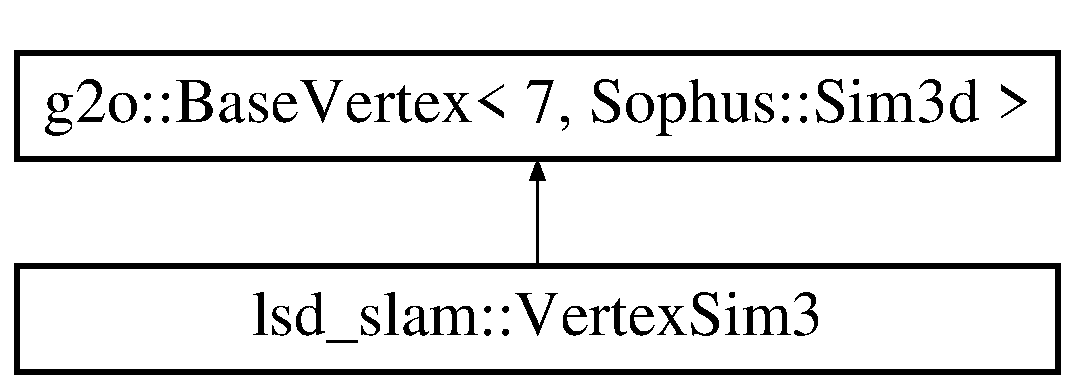
\includegraphics[height=2.000000cm]{classlsd__slam_1_1_vertex_sim3}
\end{center}
\end{figure}
\subsection*{Public Member Functions}
\begin{DoxyCompactItemize}
\item 
\hypertarget{classlsd__slam_1_1_vertex_sim3_af385a9fd972a3d93ff554c655d93eaa4}{virtual bool {\bfseries read} (std\-::istream \&is)}\label{classlsd__slam_1_1_vertex_sim3_af385a9fd972a3d93ff554c655d93eaa4}

\item 
\hypertarget{classlsd__slam_1_1_vertex_sim3_aa2a67fe0082a83262a5495f4e75dd5ae}{virtual bool {\bfseries write} (std\-::ostream \&os) const }\label{classlsd__slam_1_1_vertex_sim3_aa2a67fe0082a83262a5495f4e75dd5ae}

\item 
\hypertarget{classlsd__slam_1_1_vertex_sim3_afbd6e2b2548e3784e2ff9abe1c5d0bc9}{virtual void {\bfseries set\-To\-Origin\-Impl} ()}\label{classlsd__slam_1_1_vertex_sim3_afbd6e2b2548e3784e2ff9abe1c5d0bc9}

\item 
\hypertarget{classlsd__slam_1_1_vertex_sim3_a16e001bf528706acb8d327930c833e02}{virtual void {\bfseries oplus\-Impl} (const double $\ast$update\-\_\-)}\label{classlsd__slam_1_1_vertex_sim3_a16e001bf528706acb8d327930c833e02}

\end{DoxyCompactItemize}
\subsection*{Public Attributes}
\begin{DoxyCompactItemize}
\item 
\hypertarget{classlsd__slam_1_1_vertex_sim3_ab474766399d0a98c6d66c49433b4decc}{{\bfseries E\-I\-G\-E\-N\-\_\-\-M\-A\-K\-E\-\_\-\-A\-L\-I\-G\-N\-E\-D\-\_\-\-O\-P\-E\-R\-A\-T\-O\-R\-\_\-\-N\-E\-W}}\label{classlsd__slam_1_1_vertex_sim3_ab474766399d0a98c6d66c49433b4decc}

\item 
\hypertarget{classlsd__slam_1_1_vertex_sim3_a7090d5d90f0869db6a4c7760d9a7255e}{bool {\bfseries \-\_\-fix\-\_\-scale}}\label{classlsd__slam_1_1_vertex_sim3_a7090d5d90f0869db6a4c7760d9a7255e}

\end{DoxyCompactItemize}


The documentation for this class was generated from the following files\-:\begin{DoxyCompactItemize}
\item 
/home/king/rgbd-\/slam-\/lets-\/do-\/it/9-\/doxygen/lsd\-\_\-slam/lsd\-\_\-slam\-\_\-core/src/\-Global\-Mapping/g2o\-Type\-Sim3\-Sophus.\-h\item 
/home/king/rgbd-\/slam-\/lets-\/do-\/it/9-\/doxygen/lsd\-\_\-slam/lsd\-\_\-slam\-\_\-core/src/\-Global\-Mapping/g2o\-Type\-Sim3\-Sophus.\-cpp\end{DoxyCompactItemize}

%--- End generated contents ---

% Index
\newpage
\phantomsection
\addcontentsline{toc}{chapter}{Index}
\printindex

\end{document}
